\begin{savequote}[75mm]
Mathematics is a game played according to certain simple rules with meaningless marks on paper.
\qauthor{--- David Hilbert ---}
\end{savequote}

\chapter{Transcendental functions}
\label{chap_trans}
\graphicspath{{figures/Trans/}}

\section{Definition}
A transcendental function is a function that does not satisfy a polynomial equation, in contrast to an algebraic function. In other words, a \textbf{transcendental function} (\textit{transcendente functie}) transcends algebra in that it cannot be expressed in terms of a finite sequence of the algebraic operations of addition, multiplication, and root extraction. A function that is not transcendental is algebraic.
\index{transcendental function} \index[aut]{transcendente functie}

The most familiar transcendental functions are the logarithmic, exponential (with any non-trivial base), trigonometric, and hyperbolic functions, and the inverses of all of these. \ifcourse Less familiar are the special functions, such as the gamma, elliptic, and zeta functions. Besides, the generalized hypergeometric and Bessel functions are transcendental in general, but algebraic for some special parameter values. \fi




\section{Exponential and logarithmic functions}
\label{sec_exponential}
\subsection{Definitions}
\subsubsection{Exponential functions}
 Up to this point, we have dealt with functions that involve terms of the form  $x^{p}$ where the base of the term, $x$, varies but the exponent of each term, $p$, remains constant.  Here, we study functions of the form $f(x) = b^{x}$ where the base $b$ is a constant and the exponent $x$ is the variable.  We start our exploration of these functions with $f(x) = 2^{x}$, whose graph is shown in Figure~\ref{fig_trans_1a}.

%\renewcommand{\arraystretch}{1.5}
%\[ \begin{array}{r|ccccccc}  
%
% x &-3&-2&-1&0&1&2&3  \\[0.2cm] \hline
%f(x)& \dfrac{1}{8}&\dfrac{1}{4}& \dfrac{1}{2}&1&2&4&8\\
%\end{array} \] 
%\renewcommand{\arraystretch}{1}

\begin{figure}
\centering
%\raisebox{0.5cm}{
\centerline{
\subfigure[	\label{fig_trans_1a}]{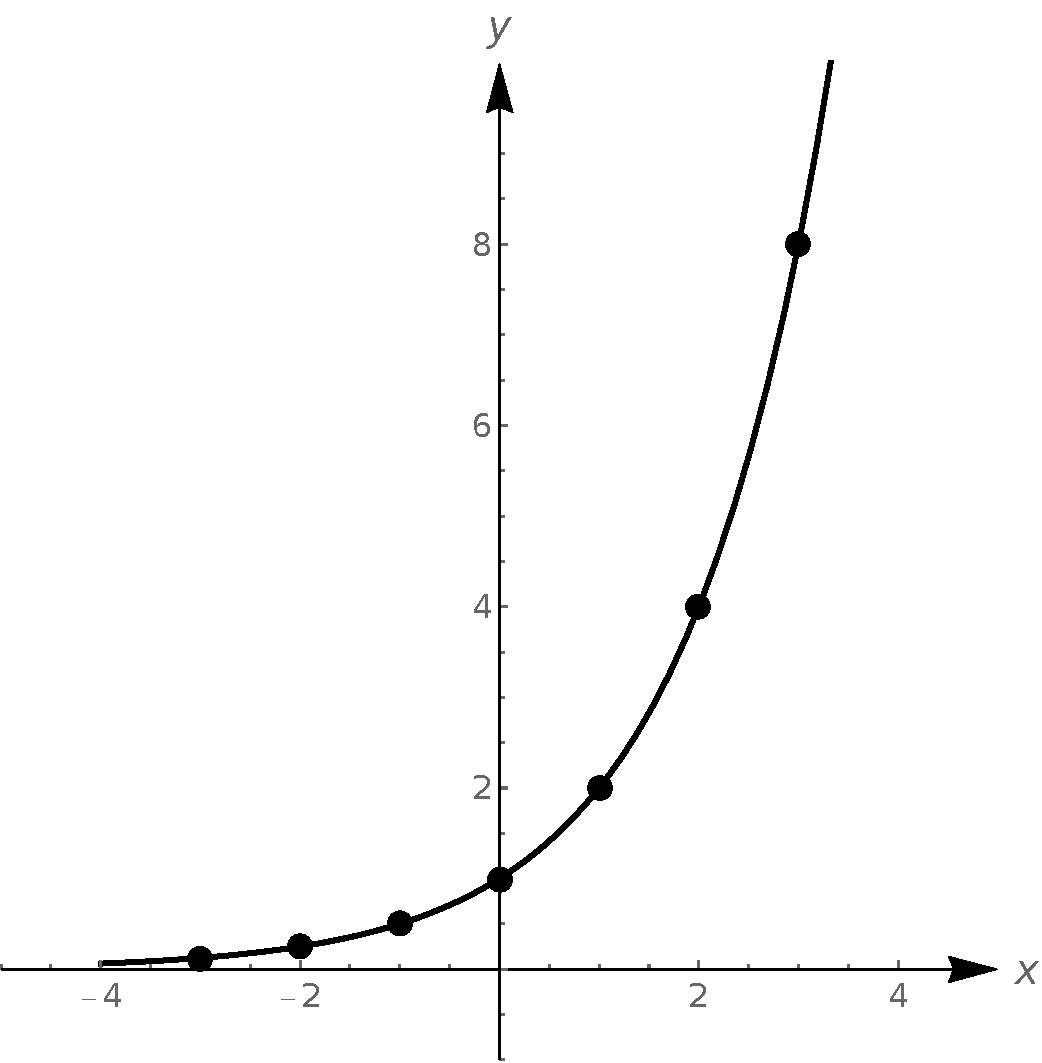
\includegraphics[width=0.4\textwidth]{fig_trans_1a}}
\hspace{1cm}
\subfigure[	\label{fig_trans_1b}]{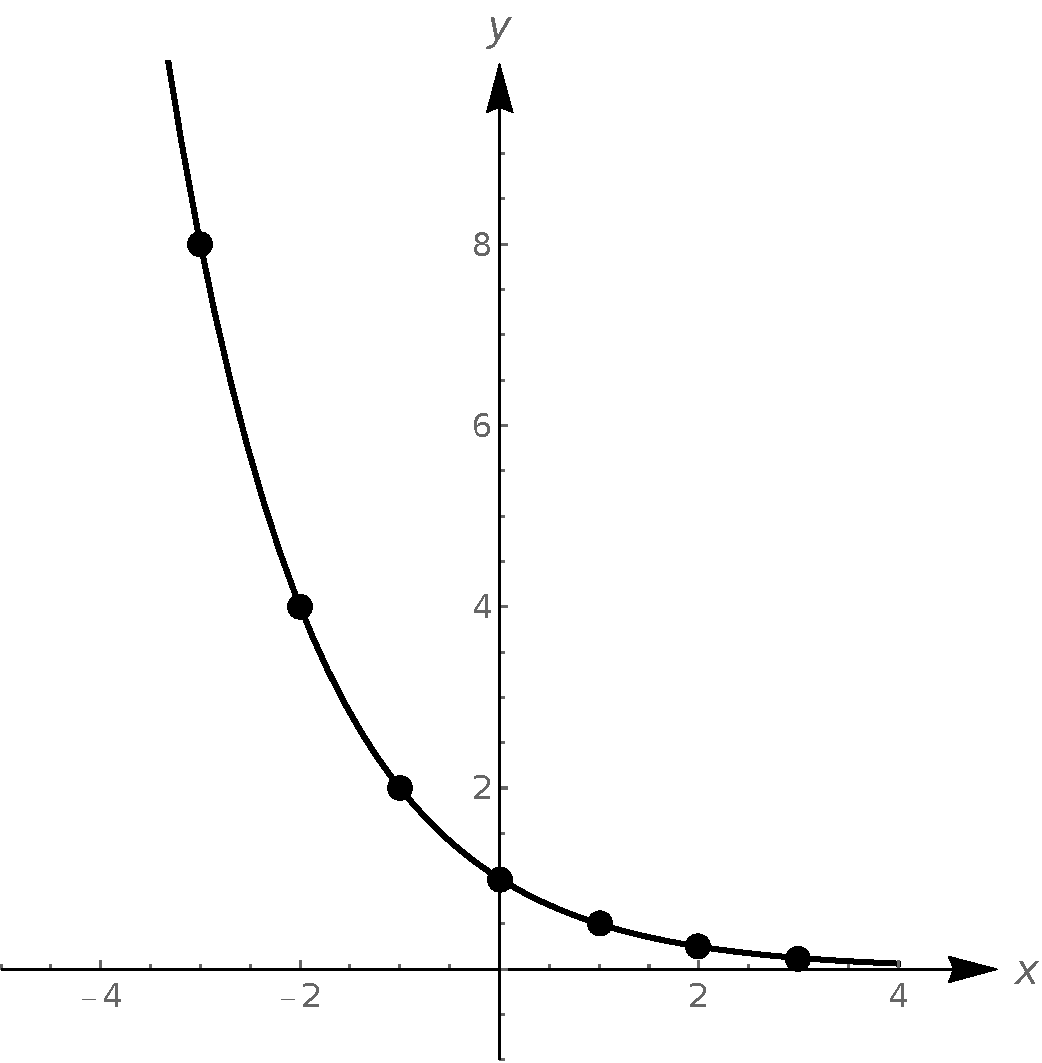
\includegraphics[width=0.4\textwidth]{fig_trans_1b}}
}	
\caption{The graph of $y=f(x)=2^x$ (a) and $y=g(x)=\left(\frac{1}{2}\right)^{x} = 2^{-x}$ (b).}
\end{figure}


A few remarks about the graph of $f(x) = 2^{x}$  are in order.  As $x \rightarrow -\infty$, the function $f(x) = 2^{x}$ takes on values that are increasingly closer to 0.  In other words, as $x \rightarrow -\infty$, $f(x) \rightarrow 0^+$ and the $x$-axis is a horizontal asymptote.  On the flip side, as $x \rightarrow +\infty$, we find $f(x) \rightarrow +\infty$. As a result, our graph suggests the range of $f$ is $\mathbb{R}^+_0$.  Besides, it is clear that $f$ is injective and hence invertible, while $\dom\,f=\mathbb{R}$. 


Here, we wish to study the family of functions $f(x) = b^{x}$, but which bases $b$ make sense to study?  We find that we run into difficulty if $b < 0$.  For example, if $b = -2$, then the function $f(x) = (-2)^{x}$ has trouble, because, for instance, at $x = \frac{1}{2}, f(x) = \sqrt{-2}$ is not a real number. So we must restrict our attention to bases $b \geq 0$.  What about $b = 0$?  The function $f(x) = 0^{x}$ is undefined for $x \leq 0$ because we cannot divide by $0$ and $0^{0}$ is an indeterminate form.  For $x > 0$, $0^{x} = 0$ so the function  $f(x) = 0^{x}$ is the same as the function $f(x) = 0$ for $x > 0$.  We know everything we can possibly know about this function, so we exclude it from our investigations.  The only other base we exclude is $b=1$, since the function $f(x) = 1^{x} = 1$ is, once again, a function we have already studied (see Chapter~\ref{chap_algebraic}). Bearing this in mind, we are now ready to give a more formal definition of exponential functions.

\begin{definition} [Exponential function]
\label{expfcndefn}  A function of the form 
$$f(x) = b^{x}\,$$ 
where $b$ is a strictly positive fixed real number ($b > 0$) and  $b \neq 1$ is called a \index{function ! exponential}\index[aut]{functie ! exponentieel}\textbf{base $b$ exponential function} (\textit{exponenti\"ele functie met grondtal $b$}). \index{base} \index[aut]{grondtal)} Moreover, such a function is called exponentially increasing if $b>1$ and exponentially decreasing if $0<b<1$. 
\end{definition}
\index{base}
\index[aut]{grondtal}



Now, we could wonder what the graph of an exponential function with  $0 < b < 1$ looks like. For instance, consider $g(x) = \left(\frac{1}{2}\right)^{x}$.  Naively, we could certainly build a table of values and connect the points, but more wisely we could take a step back and note that $g(x) = \left(\frac{1}{2}\right)^{x} = \left(2^{-1}\right)^{x} = 2^{-x} = f(-x)$, where $f(x) = 2^{x}$.  Thinking back to Section~\ref{sec_transformations}, the graph of $f(-x)$ is obtained from the graph of $f(x)$ by reflecting it across the $y$-axis (Figure~\ref{fig_trans_1b}).  We see that the domain and range of $g$ match that of $f$, namely $\mathbb{R}$ and $\mathbb{R}^+_0$, respectively. Like $f$, $g$ is also injective.  Whereas $f$ is always increasing, $g$ is always decreasing.  As a result, as $x \rightarrow -\infty$, $g(x) \rightarrow +\infty$, and on the flip side, as $x \rightarrow +\infty$, $g(x) \rightarrow 0^{+}$.  


In literature, one very often comes across the wording \textbf{exponential growth} (\textit{exponenti\"ele groei}),\index{exponential growth}\index[aut]{exponenti\"ele groei} but what exactly does it mean? Let us contrast exponential growth with linear growth in the following table. 

\renewcommand{\arraystretch}{1.5}
\[ \begin{array}{r|r|r}  
 x & f(x)=2^x & h(x)=2x \\ \hline\hline
0  &  1 & 0 \\  
1  &  2 & 2 \\  
2  & 4 & 4 \\  
3  &  8 & 6 \\  
4  & 16 & 8 \\  
5  &  32 & 10 \\  
\end{array} \]
\renewcommand{\arraystretch}{1}

From this table we can infer that for these two functions, exponential growth dwarfs linear growth. More specifically, the former implies that original value from the range increases by the same percentage over equal increments found in the domain, whereas the latter refers to the original value from the range that increases by the same amount over equal increments found in the domain.
For exponential growth, over equal increments, the constant multiplicative rate of change resulted in doubling the output whenever the input increased by one. For linear growth, the constant additive rate of change over equal increments resulted in adding 2 to the output whenever the input was increased by one.

Of all of the bases for exponential functions, two occur the most often in scientific circles.  The first, base $10$, is often called the \index{common base}\index[aut]{tiendelige basis}\textbf{common base} (\textit{tiendelige basis}).  The second base is an irrational number, $e \approx 2.718$, called the \index{natural base}\index[aut]{natuurlijke basis}\textbf{natural base}.  The following examples give us an idea how these functions are used in the wild.

\begin{example}  \label{cardepreciationex} The value of a tractor can be modelled by $V(x) = 25\left(\frac{4}{5}\right)^{x}$, where $x \geq 0$ is age of the vehicle in years and $V(x)$ is the value in thousands of euros. 

\begin{enumerate}

\item  Find and interpret $V(0)$.

\item  Sketch the graph of $y=V(x)$ using transformations.

\item  Find and interpret the horizontal asymptote of the graph of $y=V(x)$.

\end{enumerate}

\xhrulefill{gray}{2.5pt}Solution \xhrulefill{gray}{2.5pt}

\begin{enumerate}

\item  To find $V(0)$, we replace $x$ with $0$ to obtain $V(0) = 25\left(\frac{4}{5}\right)^{0} = 25$.  Since $x$ represents the age of the tractor in years, $x=0$ corresponds to the tractor being brand new.  Since $V(x)$ is measured in thousands of euros, $V(0)=25$ corresponds to a value of \euro $ 25,000$.  Putting it all together, we interpret $V(0)=25$ to mean the purchase price of the tractor was \euro $25\,000$.


\item  To graph $y=25\left(\frac{4}{5}\right)^{x}$,  we start with the basic exponential function $f(x)=\left(\frac{4}{5}\right)^{x}$.  Since the base $b = 4/5$ is between $0$ and $1$, the graph of $y=f(x)$ is decreasing.  We plot the $y$-intercept $(0,1)$ and two other points, $\left(-1, 5/4\right)$ and $\left(1, 4/5\right)$, and notice the horizontal asymptote $y=0$ (Figure~\ref{fig_trans_2a}).  To obtain $V(x) = 25\left(\frac{4}{5}\right)^{x}$, we multiply the output from $f$ by $25$, which results in a vertical stretch by a factor of $25$.  We multiply all of the $y$-values in the graph by $25$ and obtain the points $\left(-1,125/4\right)$, $(0,25)$ and $(1,20)$. The horizontal asymptote remains 0. Finally, we restrict the domain to $\mathbb{R}^+$  to fit with the applied domain given to us (Figure~\ref{fig_trans_2b}).


\item  We see from the graph of $V$ that its horizontal asymptote is $y=0$. This means as the tractor gets older, its value diminishes to $0$. 
 
\end{enumerate}

\begin{figure}[H]
\centering
%\raisebox{0.5cm}{
\centerline{
\subfigure[	\label{fig_trans_2a}]{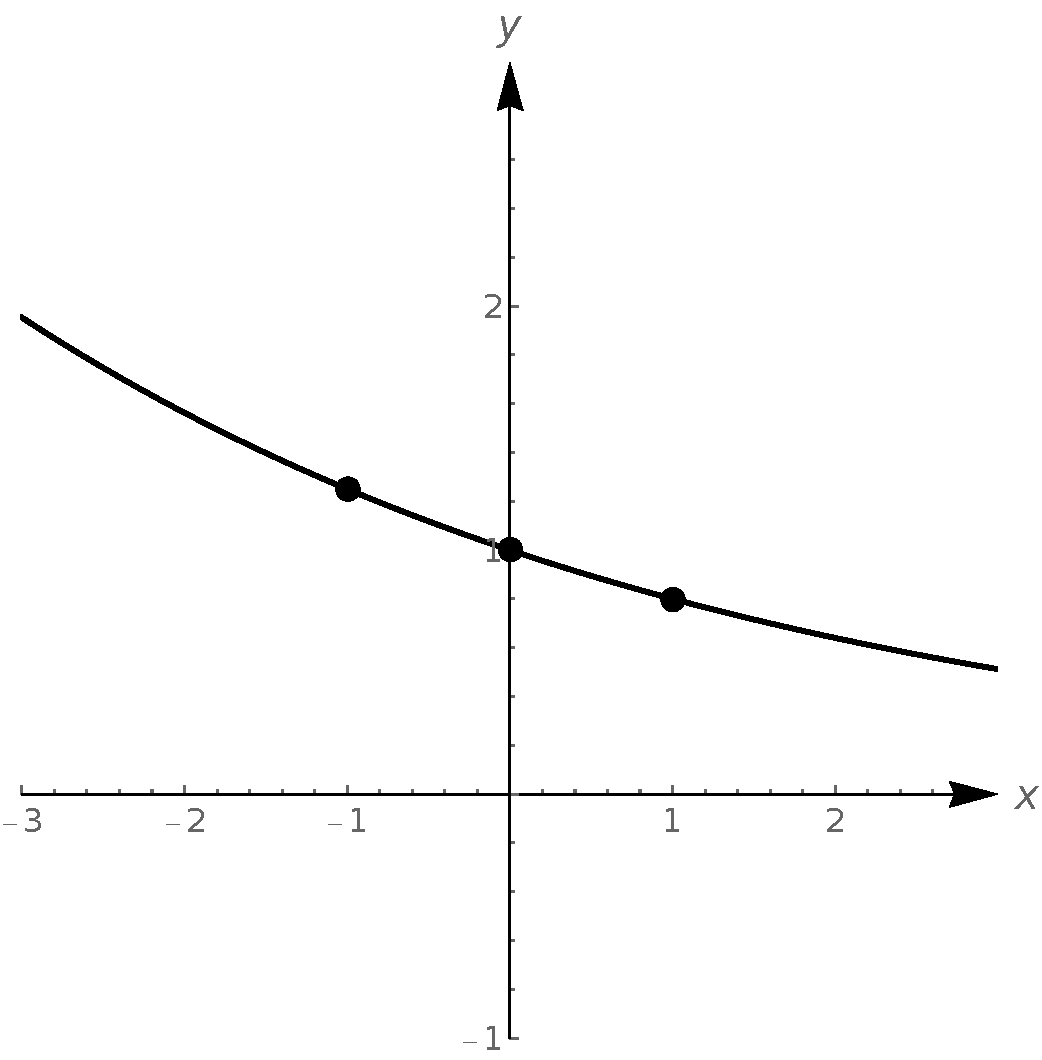
\includegraphics[width=0.4\textwidth]{fig_trans_2a}}
\hspace{1cm}
\subfigure[	\label{fig_trans_2b}]{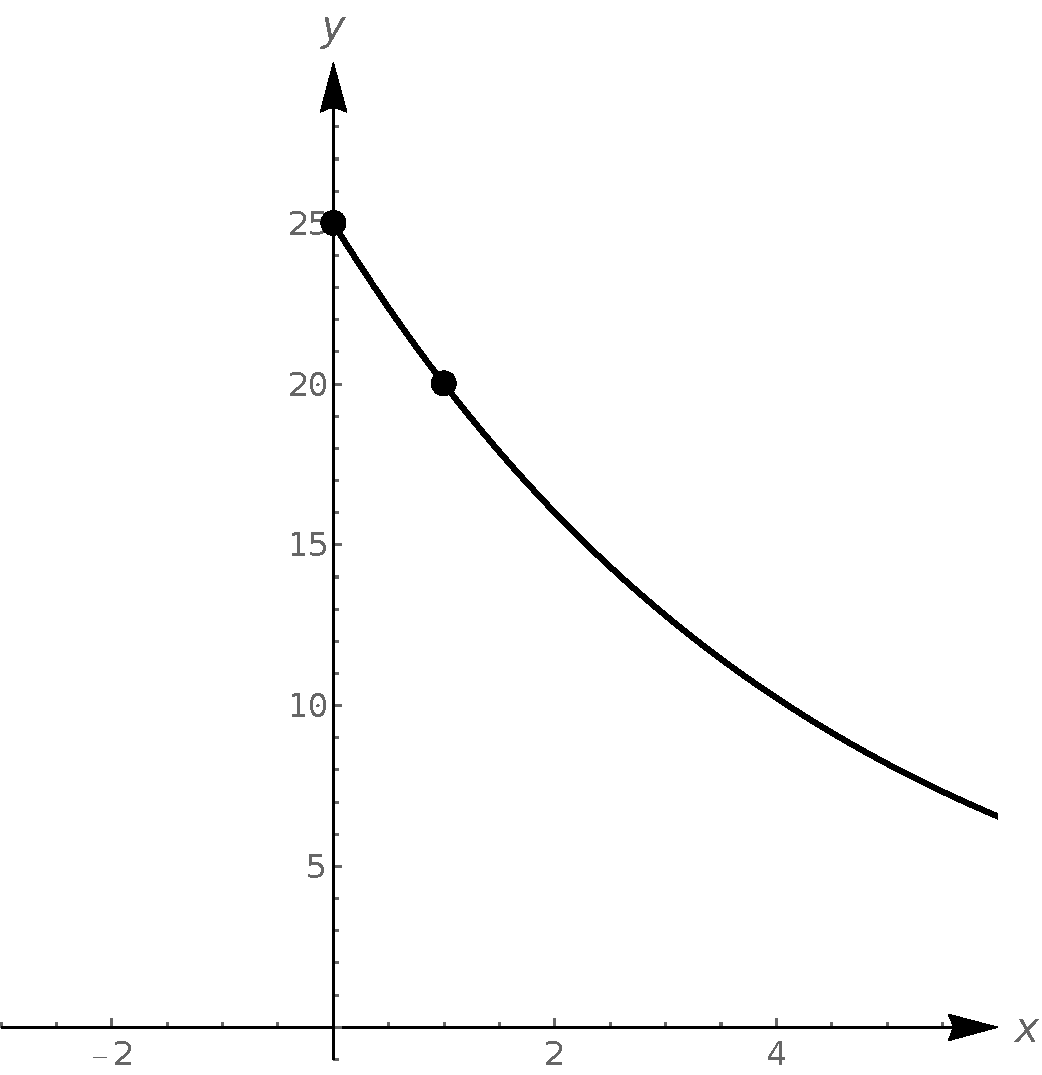
\includegraphics[width=0.4\textwidth]{fig_trans_2b}}
}	
\caption{The graph of $y=f(x)=\left(\frac{4}{5}\right)^{x}$ (a) and $y=V(x)=25\left(\frac{4}{5}\right)^{x}$ (b) in Example~\ref{cardepreciationex}.}
\end{figure}


\end{example}

\ifcourse

The function in the previous example is often called a \index{decay curve}\index[aut]{vervalkromme}\textbf{decay curve}.  In contrast, increasing exponential functions are used to model growth curves and we shall see several different examples of those later. We present another common decay curve in the following example.  Although it may look more complicated than the previous example, it is actually just a basic exponential function which has been modified by a few transformations from Section \ref{sec_transformations}.

\begin{example} 
 \label{exptempex} According to Newton's Law of cooling the temperature of coffee $T$ [$\Theta$] in degrees Celsius $t$ [T] minutes after it is served can be modelled by 
 $$T(t) = 21 + 50 e^{-0.1 t}.$$
 \index{Newton's Law of Cooling}\index[aut]{Koelingswet van Newton}

\begin{enumerate}

\item  Find and interpret $T(0)$.

\item  Sketch the graph of $y = T(t)$ using transformations.

\item  Find and interpret the horizontal asymptote of the graph.

\end{enumerate}


\xhrulefill{gray}{2.5pt}Solution \xhrulefill{gray}{2.5pt}

\begin{enumerate}

\item  To find $T(0)$, we replace every occurrence of the independent variable $t$ with $0$ to obtain  $T(0) =21 + 50 e^{-0.1 (0)} = 71$.  This means that the coffee was served at $71^{\circ}\mbox{C}$.

\item  To graph $y = T(t)$ using transformations, we start with the basic function, $f(t)=e^{t}$.  Since $e \approx~2.718~>~1$, the graph of $f$ is an increasing exponential with $y$-intercept $(0,1)$ and horizontal asymptote $y = 0$.  The points $\left(-1, e^{-1}\right) \approx (-1,0.37)$ and $(1,e) \approx (1,2.72)$ are also on the graph (Figure~\ref{fig_trans_3a}).  To use this information on $f(t)=e^{t}$, we rewrite $T(t)$ as 
 \[T(t) = 21+50 f(-0.1t)\,.\]  


Multiplication of the input to $f$, $t$, by $-0.1$ results in a horizontal expansion by a factor of $10$ as well as a reflection about the $y$-axis.  We divide each of the $x$-values of our points by $-0.1$  to obtain $\left(10,e^{-1}\right)$, $(0,1)$, and $\left(-10, e\right)$.  Since none of these changes affected the $y$-values, the horizontal asymptote remains $y = 0$.  Next, we see that the output from $f$ is being multiplied by $50$.  This results in a vertical stretch by a factor of $50$.  We multiply the $y$-coordinates by $50$ to obtain $\left(10,50e^{-1}\right)$, $(0,50)$, and $\left(-10, 50e\right)$. Obviously,  the horizontal asymptote remains $y=0$.  Finally, we add $21$ to all of the $y$-coordinates, which shifts the graph upwards to obtain $\left(10,50e^{-1} + 21\right) \approx (10, 39.39)$, $(0,71)$, and $\left(-10, 50e+ 21\right) \approx (-10,156.91)$.  Adding $21$ to the horizontal asymptote shifts it upwards as well to $y=21$.  We connect these three points and, last but not least, we restrict the domain to match the applied domain $\mathbb{R}^+$ (Figure~\ref{fig_trans_3b}).  



\item  From the graph, we see that the horizontal asymptote is $y = 21$.  As $t \rightarrow +\infty$, the term $50 e^{-0.1t}$ becomes very small.  Hence, the graph of $T$ is approaching the horizontal line $y=21$ from above.  This means that as time goes by, the temperature of the coffee is cooling to $21^{\circ}\mbox{C}$, presumably room temperature.  

\end{enumerate}


\begin{figure}[H]
\centering
%\raisebox{0.5cm}{
\centerline{
\subfigure[	\label{fig_trans_3a}]{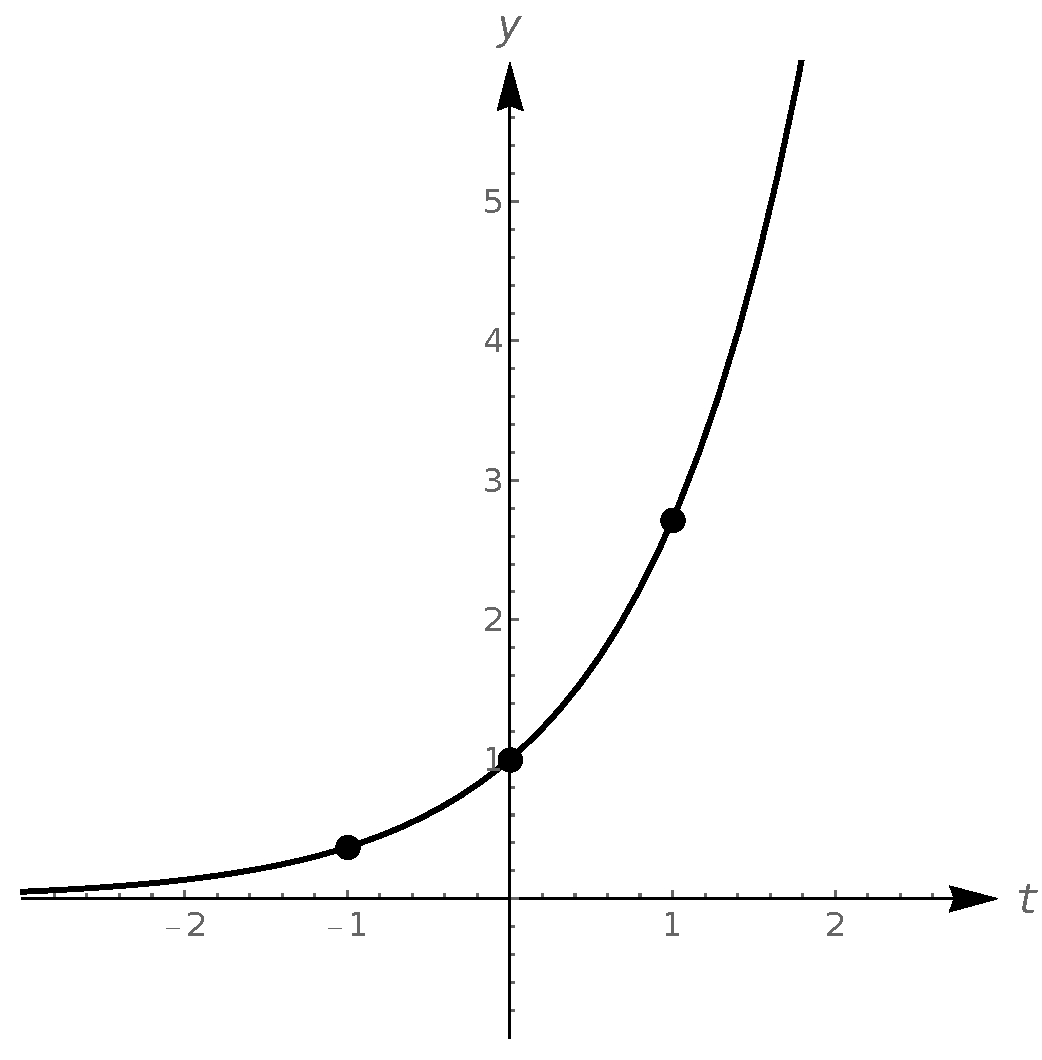
\includegraphics[width=0.4\textwidth]{fig_trans_3a}}
\hspace{1cm}
\subfigure[	\label{fig_trans_3b}]{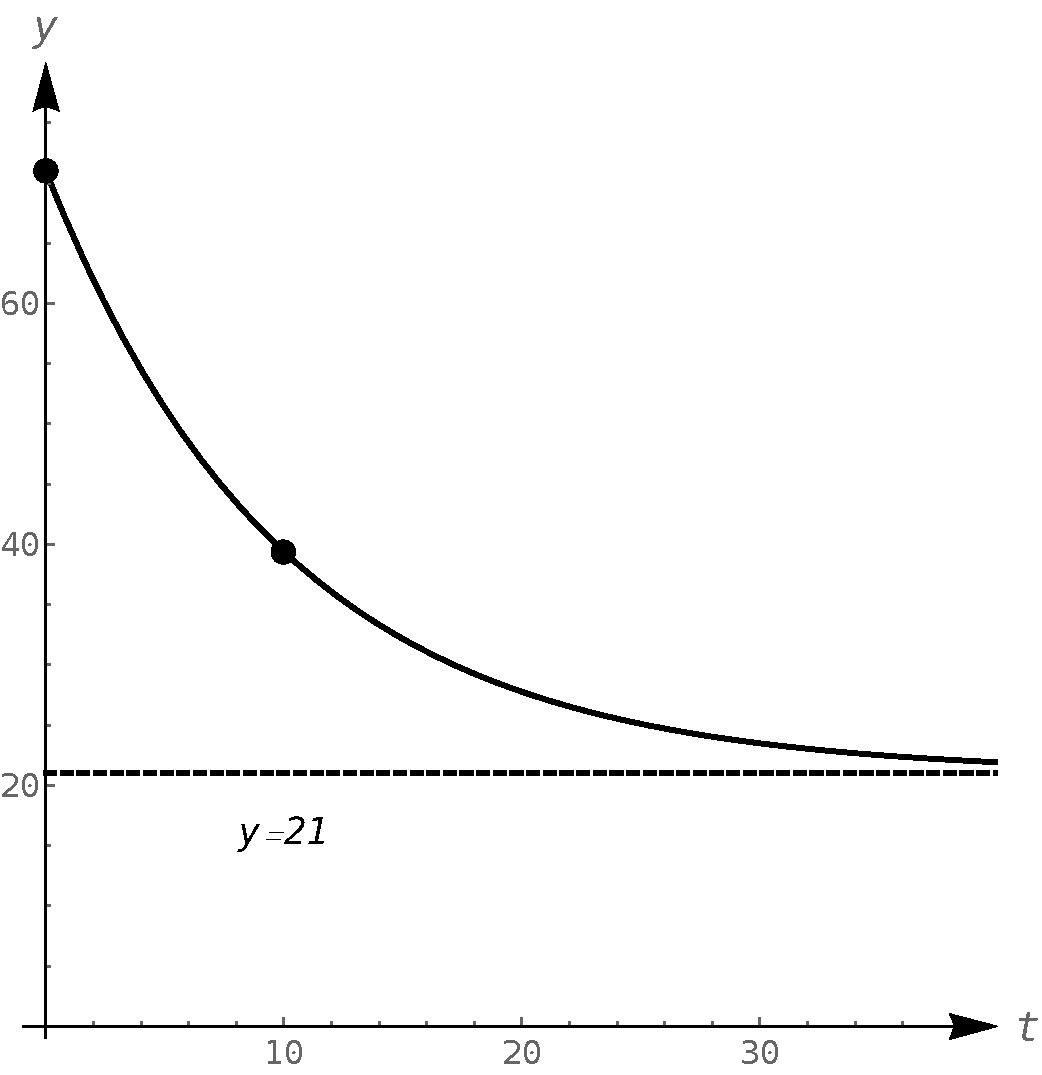
\includegraphics[width=0.4\textwidth]{fig_trans_3b}}
}	
\caption{The graph of $y=f(t)=e^{t}$ (a) and $y=T(t)=21 + 50 e^{-0.1 t}$ (b).}
\end{figure}


\end{example}

\fi 

\subsubsection{Logarithmic functions}

As we have already remarked, the function $f(x) = b^{x}$  is injective, and hence invertible.   We now turn our attention to these inverses, the logarithmic functions.


\begin{definition}[Logarithmic function]
 \label{logfcndefn} The inverse of the exponential function $f(x) = b^{x}$ is called the \index{function ! logarithmic} \textbf{base  $b$ logarithm function} (\textit{logaritmische functie met grondtal $b$}), and is denoted  
$$f^{-1}(x) = \log_{b}(x)\,.$$
We read $\log_{b}(x)$ as log base $b$ of $x$. \index{logarithm}\index[aut]{logaritme}\index{base}\index[aut]{grondtal}
\end{definition}

The \index{logarithm ! common} \textbf{common logarithm} (\textit{tiendelige logaritme, Briggse logaritme)} of a real number $x$ is $\log_{10}(x)$ and is usually written $\log(x)$.   The \index{logarithm ! natural} \textbf{natural logarithm} (\textit{natuurlijke logaritme, Neperiaanse logaritme} of a real number $x$ is $\log_{e}(x)$ and is usually written $\ln(x)$. \index{common logarithm} \index{natural logarithm}\index[aut]{logaritme ! natuurlijk}\index[aut]{logaritm ! tiendelig}


Since logarithmic functions are defined as the inverses of exponential functions, we can use the findings of Section~\ref{sec_inverse} to tell us something about logarithmic functions.  For example, we know that the domain of a logarithmic function is the range of an exponential function, namely $\mathbb{R}^+_0$, and that the range of a logarithmic function is the domain of an exponential function, namely $\mathbb{R}$.   Since we know the basic shapes of $y = f(x) = b^{x}$ for the different cases of $b$, we can obtain the graph of $y = f^{-1}(x) = \log_{b}(x)$ by reflecting the graph of $f$ across the line $y=x$ as shown below.  The $y$-intercept $(0,1)$ on the graph of $f$  corresponds to an $x$-intercept of $(1,0)$ on the graph of $f^{-1}$.  The horizontal asymptotes $y=0$ on the graphs of the exponential functions become vertical asymptotes $x=0$ on the graphs of the logarithmic functions. All this is illustrated in Figure~\ref{fig_trans_4} for the functions $f_1(x)=e^x$, $f_2(x)=2^x$, $f_3(x)=\left(\frac{1}{e}\right)^x$ and $f_4(x)=\left(\frac{1}{2}\right)^x$ and their corresponding inverses $f_1^{-1}(x)=\ln(x)$, $f_2^{-1}(x)=\log_2(x)$, $f_3^{-1}(x)=\log_{\frac{1}{e}}(x)$ and $f_4^{-1}(x)=\log_{\frac{1}{2}}(x)$, respectively.  

\begin{figure}[h]
\centering
%\raisebox{0.5cm}{
\centerline{
\subfigure[]{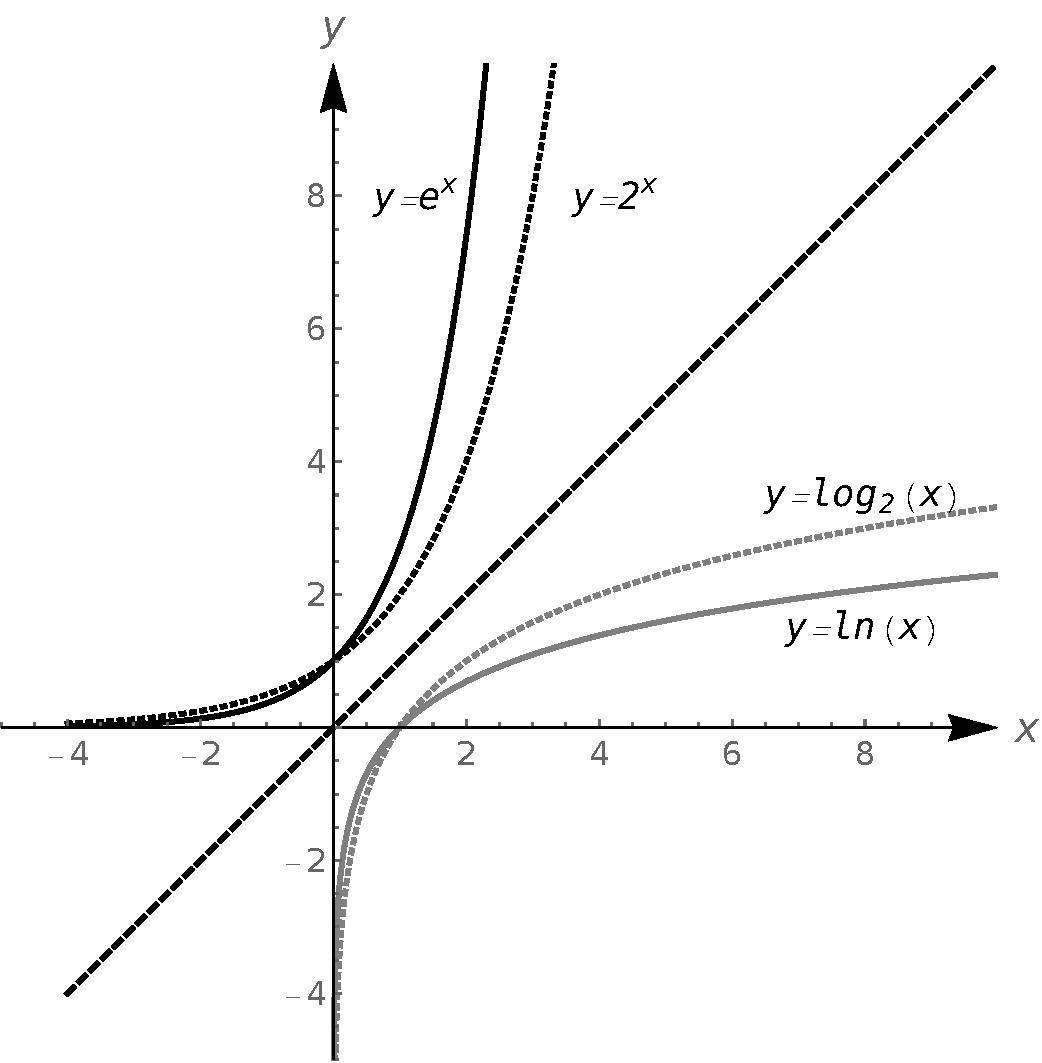
\includegraphics[width=0.4\textwidth]{fig_trans_4a}}
\hspace{1cm}
\subfigure[]{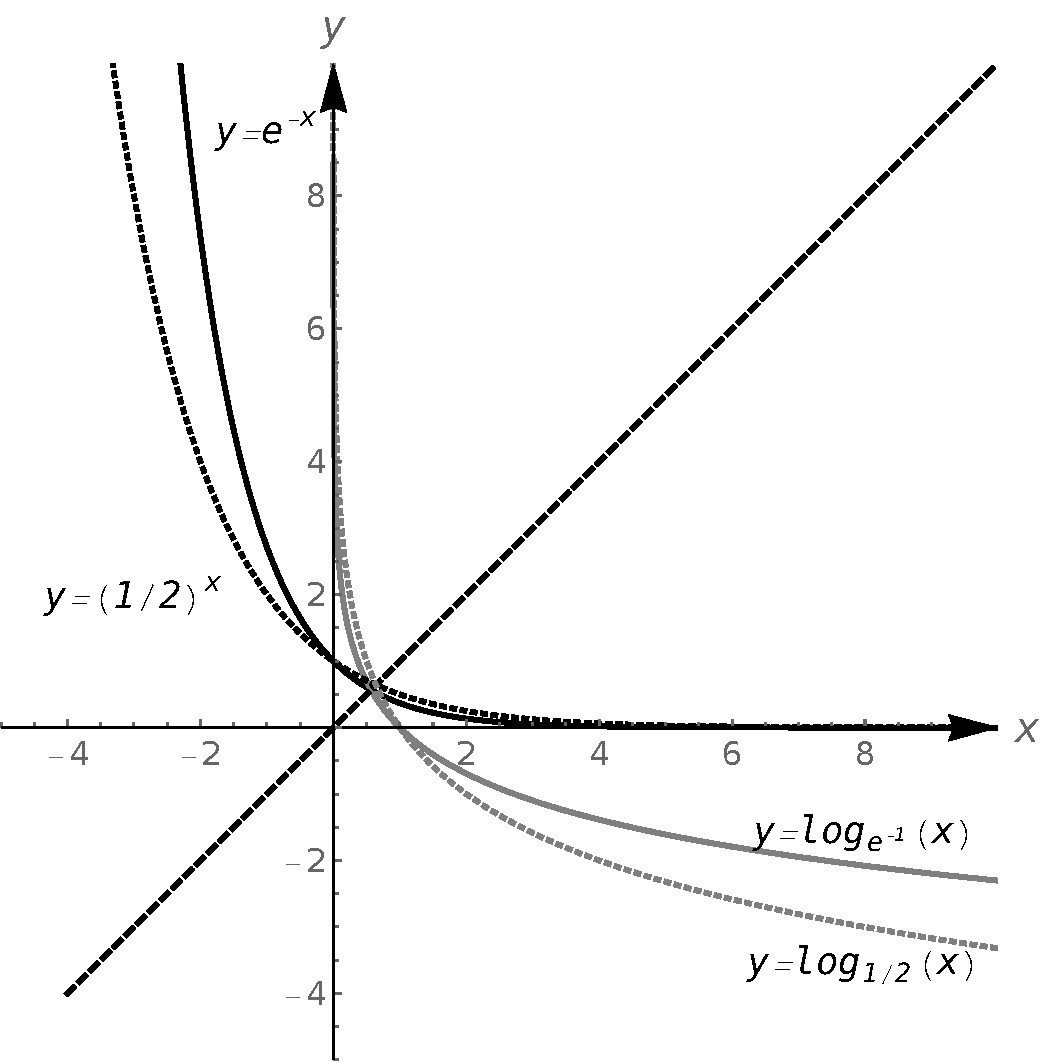
\includegraphics[width=0.4\textwidth]{fig_trans_4b}}
}	
\caption{The graph of $f_1(x)=e^x$ (a), $f_2(x)=2^x$ (a), $f_3(x)=\left(\frac{1}{e}\right)^x$ (b) and $f_4(x)=\left(\frac{1}{2}\right)^x$  (b) and their corresponding inverses $f_1^{-1}(x)=\ln(x)$ (a), $f_2^{-1}(x)=\log_2(x)$ (a), $f_3^{-1}(x)=\log_{\frac{1}{e}}(x)$ (b) and $f_4^{-1}(x)=\log_{\frac{1}{2}}(x)$ (b), respectively.}
\label{fig_trans_4}
\end{figure}

\ifcourse
\begin{remark}[Logarithms and the human psyche]
Logarithms occur in several laws describing human perception. For instance,  Hick's law proposes a logarithmic relation between the time individuals take to choose an alternative and the number of choices they have, while Fitts's law predicts that the time required to rapidly move to a target area is a logarithmic function of the distance to and the size of the target.

Interestingly, psychological studies found that individuals with little mathematics education tend to estimate quantities logarithmically, that is, they position a number on an unmarked line according to its logarithm, so that 10 is positioned as close to 100 as 100 is to 1000. Increasing education shifts this to a linear estimate that involves positioning 1000 10 times as far away.
\end{remark}

\fi




Up until this point, restrictions on the domains of functions came from avoiding division by zero and keeping negative numbers from beneath even radicals.  With the introduction of logarithmic functions, we now have another restriction.  Since the domain of $f(x) = \log_{b}(x)$ is $\mathbb{R}_0^+$, the argument  of the logarithmic function must be strictly positive.  

\ifcalculus
\begin{example}  Find the domain of the following functions.
\ifcourse 
\ifmathematica
Check your answers graphically using Mathematica.
\fi
\ifpython
Check your answers graphically using Python.
\fi
\fi

\begin{multicols}{2}
\begin{enumerate}

\item  $f(x) = 2\log(3-x)-1$

\item  $g(x) = \ln \smash{\left(\dfrac{x}{x-1}\right)}$ %\smash : compiler ignores the height of the fraction, so both items are on the same line

\end{enumerate}
\end{multicols}

\xhrulefill{gray}{2.5pt}Solution \xhrulefill{gray}{2.5pt}

\begin{enumerate}

\item  We have to make sure that the argument of the involved logarithm is strictly positive, so we set $3-x > 0$ to obtain  $\left.\right]-\infty, 3\left[\right.$.  The graph shown in Figure~\ref{fig_trans_5a} confirms this.  


\item  To find the domain of $g$, we need to solve the inequality $\frac{x}{x-1} > 0$. First, we define $r(x) = \frac{x}{x-1}$, and find that $r$ is undefined at $x=1$ and $r(x) = 0$ when $x=0$.  Choosing some test values, we easily find that $ \frac{x}{x-1} > 0$ on $\left.\right]-\infty, 0\left[\right. \cup \left.\right]1, +\infty\left[\right.$ to get the domain of $g$.  The graph of $y=g(x)$ confirms this (Figure~\ref{fig_trans_5b}). 

\end{enumerate}
\begin{figure}[H]
\centering
%\raisebox{0.5cm}{
\centerline{
\subfigure[\label{fig_trans_5a}]{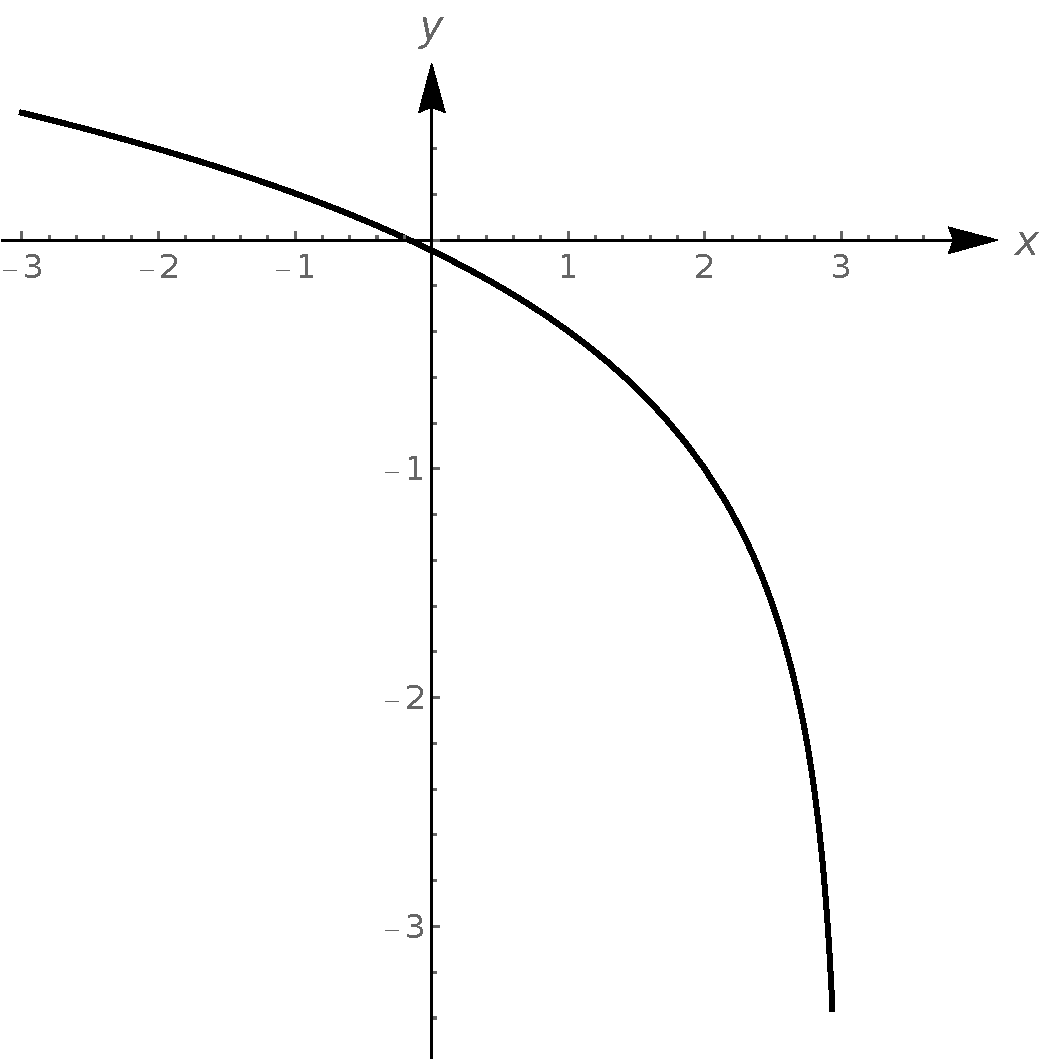
\includegraphics[width=0.4\textwidth]{fig_trans_5a}}
\hspace{1cm}
\subfigure[\label{fig_trans_5b}]{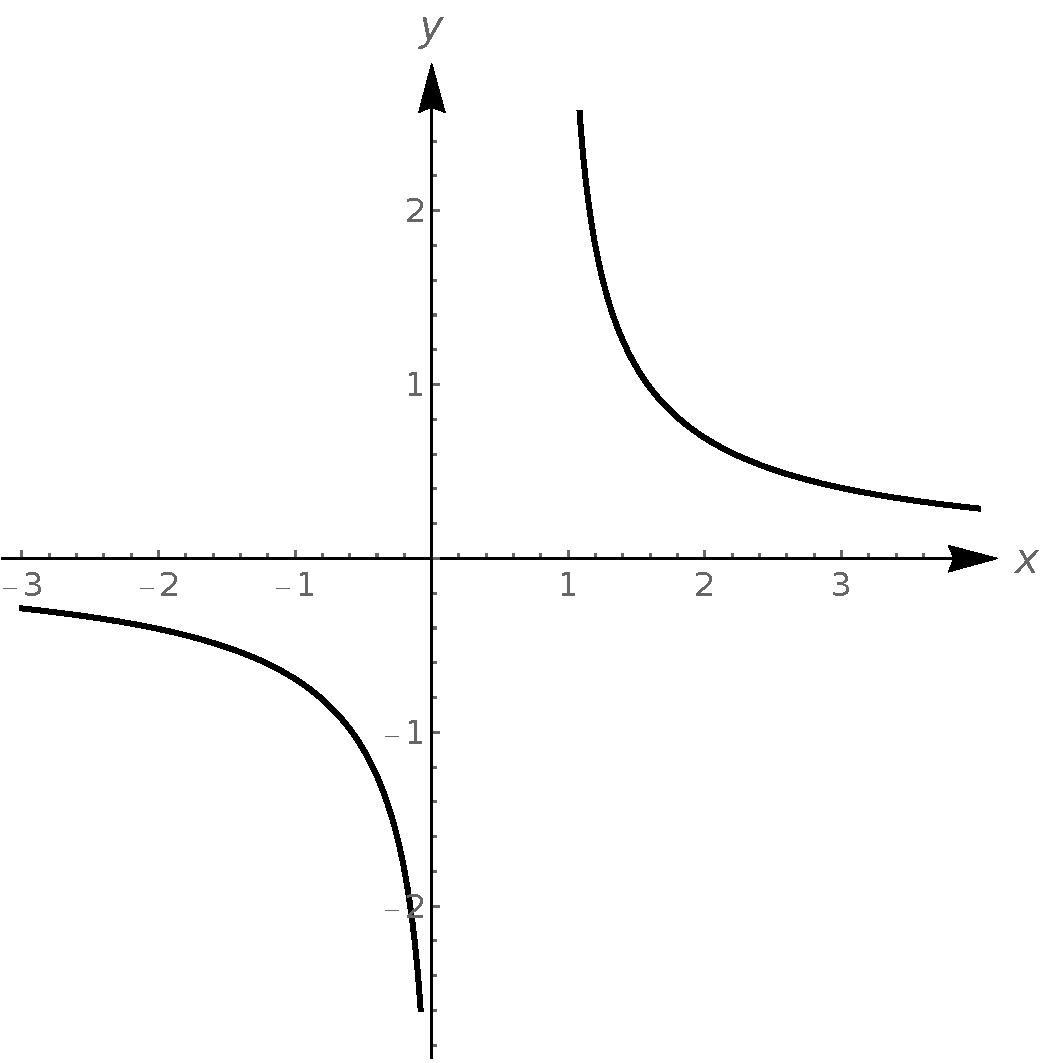
\includegraphics[width=0.4\textwidth]{fig_trans_5b}}
}	
\caption{The graph of $f(x) = 2\log(3-x)-1$ (a) and $g(x) = \ln \left(\frac{x}{x-1}\right)$ (b).}

\end{figure}


\end{example}
\fi


\subsection{Properties}
 As we shall see shortly, exponential functions inherit analogs of all of the properties of exponents you encountered in Chapter~\ref{SetsChapter}. First, we look at the consequence of  exponential and logarithmic functions to be injective.

Let $f(x) = b^{x}$ and $g(x) = \log_{b}(x)$ where $b>0$, $b\neq 1$.  Then $f$ and $g$ are injective functions and  
\begin{itemize}

\item  $b^{u} = b^{w}$ if and only if $u=w$ for all real numbers $u$ and $w$.

\item  $\log_{b}(u) = \log_{b}(w)$ if and only if $u=w$ for all real numbers $u > 0$, $w > 0$.

\end{itemize}

We now state the algebraic properties of exponential functions which will serve as a basis for the properties of logarithms.  While these properties may look identical to the ones you learned in  Chapter~\ref{SetsChapter}, they apply to real number exponents, not just rational exponents.  


\begin{theorem}[Algebraic properties of exponential functions]  \label{algpropexpfcns}  
Let $b > 0$, $b\neq 1$ and let $u$ and $w$ be real numbers, then 

\begin{itemize}

\item  \textbf{Product rule}:   $b^{u+w} = b^{u}\,b^{w}$

\item  \textbf{Quotient rule}:  $b^{u-w} = \dfrac{b^{u}}{b^{w}}$

\item  \textbf{Power rule}:   $\left(b^{u}\right)^{w} = b^{u\,w}$

\end{itemize}

\end{theorem}


To each of these properties of exponential functions corresponds an analogous property of logarithmic functions.  We list these below in our next theorem.



\begin{theorem}[Algebraic properties of logarithmic functions]  \label{algproplogfcns} 
 Let $b > 0$, $b\neq 1$ and let $u>0$ and $w>0$ be real numbers. 

\begin{itemize}

\item  \textbf{Product rule}:  $\log_{b}(u\,w) = \log_{b}(u) + \log_{b}(w)$

\item  \textbf{Quotient rule}:  $\log_{b} \left( \dfrac{u}{w} \right) = \log_{b}(u) - \log_{b}(w)$

\item  \textbf{Power rule}:  $\log_{b}\left(u^{w}\right) = w \log_{b}(u)$

\end{itemize}

\end{theorem}

From a purely functional approach, we can see the properties in Theorem \ref{algproplogfcns} as an example of how inverse functions interchange the roles of inputs in outputs.  For instance, the product rule for exponential functions given in Theorem  \ref{algpropexpfcns}, $f(u+w) = f(u)\,f(w)$, says that adding inputs results in multiplying outputs.  Hence, whatever $f^{-1}$ is, it must take the products of outputs from $f$ and return them to the sum of their respective inputs.  Since the outputs from $f$ are the inputs to $f^{-1}$ and vice-versa, we have that $f^{-1}$ must take products of its inputs to the sum of their respective outputs. This is precisely what the product rule for logarithmic functions states in Theorem \ref{algproplogfcns}.

\ifvc
\begin{example}  \label{expandlogex} Expand the following expressions using the properties of logarithms and simplify.  Assume when necessary that all quantities represent positive real numbers.

\begin{multicols}{2}
\begin{enumerate}

\item $\log_{2}\left(\dfrac{8}{x}\right)$ \vphantom{$\ln \left(\dfrac{3}{ex}\right)^2$}


\item  $\ln \left(\dfrac{3}{ex}\right)^2$

\item  $\log \sqrt[3]{\dfrac{100 x^2}{yz^5}}$

\item  $\vphantom{\log \sqrt[3]{\dfrac{100 x^2}{yz^5}}} \log_{117}\left(x^2 - 4\right)$


\end{enumerate}
\end{multicols}

\xhrulefill{gray}{2.5pt}Solution \xhrulefill{gray}{2.5pt}

\begin{enumerate}


\item  To expand $\log_{2}\left(\frac{8}{x}\right)$, we use the quotient rule identifying and simplify.

\setlength{\extrarowheight}{6pt}
\[ \begin{array}{rclr}

\log_{2}\left(\dfrac{8}{x}\right) & = &  \log_{2}(8) - \log_{2}(x) & \quad\mbox{(Quotient rule.)} \\

& = &  3 - \log_{2}(x) & \quad\mbox{(Since $2^{3} = 8$.)} \\

\end{array}\]

\setlength{\extrarowheight}{2pt}

\item  We have 

\setlength{\extrarowheight}{6pt}
\[ \begin{array}{rclr}

\ln \left(\frac{3}{ex}\right)^2 & = & 2 \ln \left(\dfrac{3}{ex}\right) & \quad\mbox{(Power rule.)} \\
                                 & = & 2 \left[ \ln(3) - \ln(ex) \right] & \quad\mbox{(Quotient rule.)} \\
                                 & = & 2 \ln(3) - 2\ln(ex) & \\
                                 & = & 2 \ln(3) - 2\left[\ln(e) + \ln(x)\right] & \quad\mbox{(Product rule.)} \\
                                 & = & 2\ln(3) - 2 - 2 \ln(x) & \quad\mbox{(Since $e^{1} = e$.)} \\
\end{array}\]
\setlength{\extrarowheight}{2pt}
                        

\item In Theorem \ref{algproplogfcns}, there is no mention of how to deal with radicals.  However, we can rewrite the cube root as a $\frac{1}{3}$ exponent.  We begin by using the Power Rule and we keep in mind that the common log is log base $10$. 
\setlength{\extrarowheight}{6pt}
\[ \begin{array}{rclr}

\log \sqrt[3]{\dfrac{100 x^2}{yz^5}} & = & \log \left(\dfrac{100 x^2}{yz^5}\right)^{1/3} & \\ [10pt]
																		& = & \frac{1}{3} \log\left(\dfrac{100 x^2}{yz^5}\right) & \quad\mbox{(Power rule.)} \\ [5pt]
																		& = & \frac{1}{3} \left[ \log\left(100x^2\right) - \log\left(yz^5\right) \right] & \quad\mbox{(Quotient rule.)} \\ 
																		& = & \frac{1}{3}\log\left(100x^2\right) - \frac{1}{3}\log\left(yz^5\right) & \\
																		& = & \frac{1}{3}\left[ \log(100) + \log\left(x^2\right)\right] - \frac{1}{3} \left[ \log(y) + \log\left(z^5\right) \right] & \quad\mbox{(Product rule.)} \\
																		& = & \frac{1}{3} \log(100) + \frac{1}{3} \log\left(x^2\right) - \frac{1}{3} \log(y) - \frac{1}{3} \log\left(z^5\right) \\
																		& = & \frac{1}{3} \log(100) + \frac{2}{3} \log(x) - \frac{1}{3} \log(y) - \frac{5}{3} \log(z) & \quad\mbox{(Power rule.)} \\
																		& = & \frac{2}{3} + \frac{2}{3} \log(x) - \frac{1}{3} \log(y) - \frac{5}{3} \log(z) &  \\

\end{array} \]
\setlength{\extrarowheight}{2pt}

\item  At first it seems as if we have no means of simplifying $\log_{117}\left(x^2-4\right)$, since none of the properties of logs addresses the issue of expanding a difference inside the logarithm.  However, we may factor $x^2 - 4 = (x+2)(x-2)$ thereby introducing a product which gives us license to use the product rule.

\setlength{\extrarowheight}{4pt}
\[ \begin{array}{rclr}

\log_{117}\left(x^2-4\right) & = & \log_{117} \left[(x+2)(x-2)\right] & \quad\mbox{(Factor.)} \\
														 & = & \log_{117}(x+2) + \log_{117}(x-2) & \quad\mbox{(Product rule.)} \\
\end{array}\]
\setlength{\extrarowheight}{2pt}

Note that the functions $f(x) = \log_{117}\left(x^2-4\right)$ and $g(x) = \log_{117}(x+2) + \log_{117}(x-2)$ have different domains, and, hence, they are different functions. We leave it to the reader to verify the domain of $f$ is $\left.\right]-\infty, -2\left[\right. \cup \left.\right]2,+\infty\left[\right.$ whereas the domain of $g$ is $\left.\right]2,+\infty\left[\right.$.
\end{enumerate}

\end{example}



Of course, the algebraic properties of exponentials and logarithms may also be used to combine logarithms. 
\fi

\begin{example}  \label{contractlogex} Use the properties of logarithms to write the following as a single logarithm.

\begin{multicols}{2}
\begin{enumerate}

\item  $\log_{3}(x-1) - \log_{3}(x+1)$

\item  $\log(x) + 2\log(y) - \log(z)$

\end{enumerate}
\end{multicols}

\xhrulefill{gray}{2.5pt}Solution \xhrulefill{gray}{2.5pt}

\ifvc Whereas in Example \ref{expandlogex} we read the properties in Theorem \ref{algproplogfcns} from left to right to expand logarithms, in this example we read them from right to left. \fi

\begin{enumerate}

\item The difference of logarithms requires the quotient rule: 
$$\log_{3}(x-1) - \log_{3}(x+1) = \log_{3}\left(\frac{x-1}{x+1}\right)\,.$$

\item  We first apply the power rule, and then the product/quotient rule to get the following.
\setlength{\extrarowheight}{6pt}
\[ \begin{array}{rclr}

\log(x) + 2\log(y) - \log(z) & = & \log(x) + \log\left(y^2\right) - \log(z) & \quad\mbox{(Power rule.)} \\ [6pt]
                             & = & \log\left(xy^2\right) - \log(z) & \quad\mbox{(Product rule.)} \\ [10pt]
                             & = & \log\left( \dfrac{xy^2}{z}\right) & \quad\mbox{(Quotient rule.)} \\
                             
                            
\end{array}\]
\setlength{\extrarowheight}{2pt}

\end{enumerate}
\end{example}


We observe that using log properties to reassemble logarithms can increase the domain of the expression.  For example, we leave it to the reader to verify the domain of $f(x) = \log_{3}(x-1) - \log_{3}(x+1)$ is $\left.\right]1,+\infty\left[\right.$ but the domain of $g(x) = \log_{3}\left(\frac{x-1}{x+1}\right)$ is $\left.\right]-\infty, -1\left[\right. \cup \left.\right]1, +\infty\left[\right.$.  We will need to keep this in mind when we solve equations involving logarithms 

In many cases it is convenient to change the base of the governing exponential or logarithmic functions. For that purpose, we may rely on the following theorem. 

\begin{theorem}[Change of base formulas] \label{changeofbase}  
Let $a,b >0$, and $a,b \neq 1$. Then, we have \index{change of base formulas} \index{exponential function ! change of base formula} 

\begin{itemize}

\item  $a^{x} = b^{x \log_{b}(a)}$, for all real numbers $x$;

\item  $\log_{a}(x) = \dfrac{\log_{b}(x)}{\log_{b}(a)}$, for all real numbers $x > 0$.

\end{itemize}

\end{theorem}

\ifanalysis

\begin{proof}
The proof of Theorem~\ref{changeofbase} is a result of the properties studied earlier.  For instance, if we start with $b^{x \log_{b}(a)}$ and use the power rule in the exponent to rewrite $x \log_{b}(a)$ as $\log_{b}\left(a^{x}\right)$ and then apply one of the inverse properties, we get \[ b^{x \log_{b}(a)} = b^{\log_{b}\left(a^{x}\right)} = a^{x},\] as required. 

To verify the logarithmic form of the property, we also use the power rule and an inverse property. We note that \[\log_{a}(x) \, \log_{b}(a) =  \log_{b} \left(a^{\log_{a}(x)}\right) = \log_{b}(x),\] and we get the result by dividing through by $\log_{b}(a)$.  Note the inverse relationship between these two change of base formulas.  To change the base of an exponential expression, we multiply the input by the factor $\log_{b}(a)$.  To change the base of a logarithmic expression, we divide the output by the factor $\log_{b}(a)$.  
\end{proof}

\fi

\subsection{Exponential and logarithmic equations and inequalities}
In this section we will briefly recall techniques for solving equations involving exponential or logarithmic functions.  We first summarize below the two common ways to solve exponential equations.

\begin{enumerate}

\item  Isolate the exponential function.

\item  \begin{enumerate}

\item  If convenient, express both sides with a common base and equate the exponents.

\item  Otherwise, take the natural log of both sides of the equation and use the power rule.


\end{enumerate}
\end{enumerate}
 
Likewise, the steps for solving an equation involving logarithmic functions are:

\begin{enumerate}

\item  Isolate the logarithmic function.

\item  \begin{enumerate}

\item  If convenient, express both sides as logs with the same base and equate the arguments of the log functions.

\item  Otherwise, rewrite the log equation as an exponential equation.


\end{enumerate}
\end{enumerate}




\ifcourse
\begin{remark}[Dual meaning of $\log(x)$]
Throughout this text we adopted the notation $\ln(x)$ and $\log(x)$ to refer to the natural algorithm and common logarithm of $x$, respectively. In literature and on the Internet, however, one often finds that $\log(x)$ is used to refer to the natural logarithm of $x$, so beware when consulting other sources of information! 
\end{remark}
\fi



\begin{example}  \label{expeqnsex1} Solve the following exponential and logarithmic equations.  

\begin{multicols}{2}
\begin{enumerate}

\item  $2^{3x} = 16^{1-x}$

\item  $9 \cdot 3^{x} = 7^{2x}$

\item  $75 = \dfrac{100}{1 + 3e^{-2t}}$

 \item $\log_{117}(1-3x) = \log_{117}\left(x^2-3\right)$

\item  $\log_{7}(1-2x) = 1 - \log_{7}(3-x)$

\item  $1 + 2 \log_{4}(x+1) = 2 \log_{2}(x)$

\end{enumerate}
\end{multicols}

\xhrulefill{gray}{2.5pt}Solution \xhrulefill{gray}{2.5pt}
\begin{enumerate}

\item  Since $16$ is a power of $2$, we can rewrite the equation as $2^{3x} = \left(2^4\right)^{1-x}$.  Using properties of exponents, we get $2^{3x} = 2^{4(1-x)}$.  Given the one-to-one property of exponential functions, we get $3x = 4(1-x)$, which gives $x=4/7$.


\item  We first note that we can rewrite the equation as $3^2 \cdot 3^x = 7^{2x}$ to obtain $3^{x+2} = 7^{2x}$.  Since it is not convenient to express both sides as a power of $3$ (or $7$ for that matter) we use the natural log:  $\ln\left(3^{x+2}\right) = \ln\left(7^{2x}\right)$.  The power rule gives $(x+2) \ln(3) = 2x \ln(7)$. This equation  is linear and can be solved for $x$:

\[ \begin{array}{rrclr}
&(x+2) \ln(3) & = & 2x \ln(7) & \\

\Leftrightarrow&x \ln(3) + 2 \ln(3) & = & 2x \ln(7) & \\
\Leftrightarrow&2 \ln(3) & = & 2x \ln(7) - x \ln(3) & \\
\Leftrightarrow&2 \ln(3) & = & x (2 \ln(7) - \ln(3)) &\\
\Leftrightarrow&x & = & \dfrac{2 \ln(3)}{2\ln(7) - \ln(3)} & \\ [4pt]
\end{array}\]


\item  First, we isolate the exponential:
$$
\begin{array}{rcl}
75=\dfrac{100}{1+3e^{-2t}}&\Leftrightarrow&75\left(1 + 3e^{-2t}\right) = 100\\[0.2cm]
&\Leftrightarrow&e^{-2t} = \frac{1}{9}\,.
\end{array}
$$
Taking the natural log of both sides gives 
$$\ln\left(e^{-2t}\right) = \ln\left( \frac{1}{9} \right)\quad\Leftrightarrow\quad t=\ln(3)\,.$$ 

\item  Since we have the same base on both sides of this equation , we equate what is inside the logs to get $1-3x = x^2-3$.  Solving $x^2+3x-4 = 0$ gives $x=-4$ and $x=1$.   To check whether none of these is an extraneous solution, we substitute, for instance $x=1$, into our original equation to obtain  $\log_{117}(-2) =  \log_{117}(-2)$.  While these expressions look identical, neither is a real number, which means $x=1$ is not in the domain of the original equation, and is not a solution. Similarly, we can verify that $x=-4$ is indeed a solution in the domain of the original equation. 

\item We first collect the logarithms on the same side and then use the product rule to get 
$$\log_{7}[(1-2x)(3-x)]=1\quad \Leftrightarrow\quad 7^{1} = (1-2x)(3-x)\,,$$ 
 which leads to  $2x^2-7x-4=0$ whose solution is  $x = -1/2$ or $x=4$.  However, checking $x=4$ in the original equation produces $\log_{7}(-7) = 1 - \log_{7}(-1)$, which is a clear domain violation.

\item We gather the logs to one side to get $1 = 2 \log_{2}(x) - 2 \log_{4}(x+1)$.  Before we can combine the logarithms, however, we need a common base.  Since $4$ is a power of $2$, we change the base \[\log_{4}(x+1) = \frac{\log_{2}(x+1)}{\log_{2}(4)} = \dfrac{1}{2} \log_{2}(x+1)\,.\] Hence, our original equation becomes  

\[ \begin{array}{rrclr}

&1 & = & 2 \log_{2}(x) - 2 \left(\frac{1}{2} \log_{2}(x+1)\right) & \\ [2pt]
\Leftrightarrow&1 &= & 2\log_{2}(x) - \log_{2}(x+1) & \\ [2pt]
\Leftrightarrow&1 & = & \log_{2}\left(x^2\right) - \log_{2}(x+1) & \quad\text{(Power rule.)} \\ [6pt]
\Leftrightarrow&1 & = & \log_{2}\left( \dfrac{x^{2}}{x+1}\right) & \quad\text{(Quotient rule.)} \\ \end{array}\]

Rewriting this in exponential form, we get $ \frac{x^{2}}{x+1} = 2$ or $x^2 -2x-2 = 0$.  Using the quadratic formula, we get $x = 1 \pm \sqrt{3}$. Yet, for what concerns the solution $x = 1 - \sqrt{3}$, it holds that is negative so if substituted into the original equation, the term $2 \log_{2}\left(1 - \sqrt{3}\right)$ is undefined, and hence we should discard it as solution.

\end{enumerate}


\end{example}


This example demonstrates the importance of checking for extraneous solutions when solving equations involving logarithms.  These are easy to spot - any supposed solution which causes a negative number inside a logarithm needs to be discarded.  


Just as we encountered for algebraic functions, we can also run into inequalities involving exponential or logarithmic functions.

\begin{example}  Solve the following inequalities. 
\label{expineq}
\begin{multicols}{2}

\begin{enumerate}
\item  $\dfrac{e^{x}}{e^{x}-4} \leq 3$

\item  $2^{x^2-3x} - 16 \geq 0$


\item  $\dfrac{1}{\ln(x)+1} \leq 1$

\item  $x \log(x+1) \geq x$

\end{enumerate}

\end{multicols}

\xhrulefill{gray}{2.5pt}Solution \xhrulefill{gray}{2.5pt}

\begin{enumerate}


\item The first step we need to take to solve  $\frac{e^{x}}{e^{x}-4} \leq 3$ is to get $0$ on one side of the inequality. To that end, we subtract $3$ from both sides and get .


\setlength{\extrarowheight}{12pt}
\[ \begin{array}{rclr}


&\dfrac{e^{x}}{e^{x}-4} - 3 & \leq & 0 \\

\Leftrightarrow&\dfrac{e^{x}}{e^{x}-4} - \dfrac{3 \left(e^{x}-4\right)}{e^{x}-4} & \leq & 0  \\

\Leftrightarrow&\dfrac{12 - 2e^{x}}{e^{x}-4} & \leq & 0  \\

\end{array}\]
\setlength{\extrarowheight}{2pt}

We set $r(x) = \frac{12 - 2e^{x}}{e^{x}-4}$ and we note that $r$ is undefined when its denominator $e^{x}-4=0$, or when $e^{x} = 4$.  Solving this gives $x = \ln(4)$, so the domain of $r$ is $\mathbb{R}\setminus\{\ln(4)\}$. To find the zeros of $r$, we solve $r(x) = 0$ and obtain $12 - 2e^{x} = 0$.  Solving for $e^{x}$, we find $e^{x} = 6$, or $x = \ln(6)$.  When we build our sign diagram, finding test values may be a little tricky since we need to check values around $\ln(4)$ and $\ln(6)$.  Recall that the function $\ln(x)$ is increasing which means $\ln(3) < \ln(4) < \ln(5) < \ln(6) < \ln(7)$.  While the prospect of determining the sign of $r\left(\ln(3)\right)$ may be very unsettling, remember that $e^{\ln(3)} = 3$, so \[r\left(\ln(3)\right) = \frac{12 - 2e^{\ln(3)}}{e^{\ln(3)}-4} = \frac{12-2(3)}{3-4} = -6\]  We determine the signs of $r\left(\ln(5)\right)$ and $r\left(\ln(7)\right)$ similarly and obtain the following sign diagram.

$$
\sgchart{~\ln(4) ,  \ln(6)} {\dfrac{12 - 2e^{x}}{e^{x}-4}: -+-}
$$
 From this sign diagram, we find our answer to be $\left.\right]-\infty,\ln(4)\left[\right. \cup [\ln(6), +\infty\left[\right.$. 

\item  Since we already have $0$ on one side of the inequality, we set $r(x) = 2^{x^2-3x} - 16$.  The domain of $r$ is all real numbers, so in order to construct our sign diagram, we need to find the zeros of $r$.  Setting $r(x) = 0$ gives 
$$2^{x^2-3x} = 16\quad \Leftrightarrow\quad 2^{x^2-3x} = 2^{4}\,.$$
So, $x^2 -3x = 4$ and the solutions of this equation are $x=4$ and $x=-1$.  From the sign diagram, 

$$\sgchart{-1, 4} {x^2-3x-4: +-+}$$


we see $r(x) \geq 0$ on $\left.\right]-\infty, -1] \cup [4, +\infty\left[\right.$ because $2^x$ is increasing everywhere and $x^2-3x+4$ is positive there.



\item  We start solving this inequality by getting $0$ on one side.   Getting a common denominator yields 
$$\dfrac{1}{\ln(x)+1}  - \dfrac{\ln(x)+1}{\ln(x)+1} \leq 0\quad\Leftrightarrow\quad  \frac{\ln(x)}{\ln(x)+1} \geq 0.$$  We define $r(x) = \frac{\ln(x)}{\ln(x)+1}$ and set about finding the domain and the zeros of $r$.  Due to the appearance of the term $\ln(x)$, we require  $x > 0$.  In order to keep the denominator away from zero, we solve $\ln(x)+1 = 0$ so $\ln(x) = -1$, so $x = e^{-1}$.  Hence, the domain of $r$ is $\left.\right]0, e^{-1}\left[\right. \cup \left.\right]e^{-1}, +\infty\left[\right.$.  To find the zeros of $r$, we set $r(x) = 0$ so that $\ln(x) = 0$, and we find $x = e^{0} = 1$.  In order to determine test values for $r$, we need to find numbers between $0$, $e^{-1}$, and $1$ which have a base of $e$.  Since $e \approx 2.718 > 1$, $0 < e^{-2} < e^{-1} < e^{-1/2} < 1 < e$.  To determine the sign of $r\left( e^{-2} \right)$, we use the fact that $\ln\left(e^{-2}\right)  = -2$, and find $r\left( e^{-2}\right) = \frac{-2}{-2+1} = 2$, which is positive.  The rest of the test values are determined similarly. 

$$
\sgchart{~e^{-1}, 1} {\dfrac{\ln(x)}{\ln(x)+1}: +-+}
$$
  From our sign diagram, we find the solution to be $\left.\right]0, e^{-1}\left[\right. \cup [1, +\infty\left[\right.$. 

\item  We begin by subtracting $x$ from both sides to get $x \log(x+1)  - x \geq 0$.  We define $r(x) = x \log(x+1)  - x $ and due to the presence of the logarithm, we require $x+1 > 0$, or $x > -1$.  To find the zeros of $r$, we solve $r(x)=0$ for $x$:
$$
x \log(x+1)  - x = 0\quad\Leftrightarrow\quad x \left(\log(x+1) - 1\right) = 0\,.$$
 This gives $x=0$ or $\log(x+1) - 1=0$, where the latter means that  $x = 9$.  We select test values $x$ so that $x+1$ is a power of $10$, and we obtain $-1 < -0.9 < 0 < \sqrt{10} -1 < 9 < 99$:

$$
\sgchart{0,9} {x \log(x+1)  - x: +-+}
$$
 Our sign diagram gives the solution to be $\left.\right]-1,0] \cup [9, +\infty\left[\right.$. 


\end{enumerate}


\end{example}

%\ifcourse
%
%We conclude this section with an example that could come straight from your chemistry course.
%
%\begin{example}
%The pH [--] of a solution is a measure of its acidity or alkalinity.  Specifically, we have
% $$\mbox{pH} = -\log[\mbox{H}^{+}]\,,$$ 
%where $[\mbox{H}^{+}]$ is the hydrogen ion concentration in moles per litre.  A solution with a pH less than 7 is an acid, one with a pH greater than 7 is a base (alkaline) and a pH of 7 is regarded as neutral. 
%
%Now, consider an experimental setting involving the breeding of water fleas (\textit{Daphnia sp.}). In order to successfully breed this organism the pH of a freshwater tank must be at least 7.8 but can be no more than 8.5.  Determine the corresponding range of hydrogen ion concentration.
%
%\xhrulefill{gray}{2.5pt}Solution \xhrulefill{gray}{2.5pt}
%
% We require $7.8 \leq -\log[\mbox{H}^{+}] \leq 8.5$ or $-7.8 \geq \log[\mbox{H}^{+}] \geq -8.5$.  To solve this compound inequality we solve $-7.8 \geq \log[\mbox{H}^{+}]$ and $ \log[\mbox{H}^{+}] \geq -8.5$ and take the intersection of the solution sets.  The former inequality yields $0 < [\mbox{H}^{+}] \leq 10^{-7.8}$ and the latter yields $[\mbox{H}^{+}] \geq 10^{-8.5}$.  Taking the intersection gives us our final answer $10^{-8.5} \leq [\mbox{H}^{+}] \leq 10^{-7.8}$.  
%\end{example}
%\fi



\ifcourse

\ifanalysis\pagebreak\fi
\subsection{Applications}
Exponential and logarithmic functions are used to model a wide variety of behaviours in the real world. 

\subsubsection{Growth models}
The law of uninhibited - Malthusian - growth states as its premise that the instantaneous rate at which a population increases at any time is directly proportional to the population at that time.  In other words, the more organisms there are at a given moment, the faster they reproduce.  Formulating the law as stated results in a so-called differential equation, which is the logic of Mathematics III. Anyhow, solving this differential equation leads to the following model equation for the number of organisms $N$ [-] at time $t$ [$T$]:
\begin{equation}
N(t) = N_{0}e^{kt},
\label{lawofuninhibitedgrowth}
\end{equation}
where $N(0) = N_0$ [--] is the initial number of organisms and $k>0$ is the constant of proportionality, and represents the Malthusian growth rate [$T^{-1}$]. 


\begin{example}
  In order to perform atherosclerosis research, epithelial cells are harvested from discarded umbilical tissue and grown in the laboratory.  A technician observes that a culture of $12\,000$ cells grows to $5\,000\,000$ cells in one week.  Assuming that the cells follow the law of uninhibited growth, find a formula for the number of cells, $N$, in thousands, after $t$ days.


\xhrulefill{gray}{2.5pt}Solution \xhrulefill{gray}{2.5pt}

   Since $N$ is to give the number of cells in thousands, we have $N_{0} = 12$, so $N(t) = 12e^{kt}$.  In order to complete the formula, we need to determine the growth rate $k$.  We know that after one week, the number of cells has grown to five million.  Since $t$ measures days and the units of $N$ are in thousands, this translates mathematically to $N(7) = 5000$.  We get the equation $12e^{7k} = 5000$ which gives $k = \frac{1}{7} \ln\left(\frac{1250}{3}\right)$.  Hence, we get $$N(t) = 12e^{ \frac{t}{7} \ln\left(\frac{1250}{3}\right)}.$$
  Of course, in practice, we would approximate $k$ to some desired accuracy, say $k \approx 0.8618$, which we can interpret as an $86.18 \%$ daily growth rate for the cells. 

\end{example}

Obviously, the law of uninhibited growth will in most practical settings not hold because the availability of resources in the environment that are needed for organisms to grow and persist is limited. This effect can, however, be incorporated in a logistic - Verhulst - growth model, which incorporates that the rate of growth of a population varies jointly with the population itself as well as the room the population has to grow.  More specifically,  if a population behaves according to the assumptions of \textbf{logistic growth} (\textit{logistische groei}), the number of organisms $N$ [-] at time $t$ [$T$] is given by 
\begin{equation}
N(t) =\dfrac{L}{1 + Ce^{-kLt}},
\label{logisticgrowth}
\end{equation}
where $N(0) = N_0$ is the initial population,  $L$ [--] is the limiting population, $C$ [--] is a measure of how much room there is to grow given by 
\[C = \dfrac{L}{N_{\mbox{\tiny$0$}}} - 1.\]
 and $k > 0$ is the constant of proportionality [T$^{-1}$]. 

The logistic function is used not only to model the growth of organisms, but is also to model the spread of disease and rumours.

\index{logistic growth} \index[aut]{logistische groei}

\begin{example} The number of people $N$, in hundreds, at a local community college who have heard the rumour `Carl is afraid of Virginia Woolf' can be modelled using the logistic equation

\[N(t) = \dfrac{84}{1+2799e^{-t}},\]

where $t\geq 0$ is the number of days after April 1, 2009.


\begin{enumerate}

\item  Find and interpret $N(0)$.

\item  Find and interpret the end behaviour of $N(t)$. 

\item  How long until $4200$ people have heard the rumour?


\end{enumerate}

\xhrulefill{gray}{2.5pt}Solution \xhrulefill{gray}{2.5pt}

\begin{enumerate}

\item  We find $N(0) = \frac{84}{1+2799e^{0}} = \frac{84}{2800} = \frac{3}{100}$.  Since $N(t)$ measures the number of people who have heard the rumour in hundreds, $N(0)$ corresponds to $3$ people.  Since $t=0$ corresponds to April 1, 2009, we may conclude that on that day, $3$ people have heard the rumour.

\item  We could simply note that $N(t)$ is written in the form of Equation~\eqref{logisticgrowth}, and identify $L = 84$.  However, to see why the answer is $84$, we proceed analytically.  Since the domain of $N$ is restricted to $t \geq 0$, the only end behaviour of significance is $t \rightarrow +\infty$. As we have seen before, as $t \rightarrow +\infty$, we have $2799 e^{-t} \rightarrow 0^{+}$ and so $N(t) \approx 84$.  Hence, as $t \rightarrow +\infty$, $N(t) \rightarrow 84$.   This means that as time goes by, the number of people who will have heard the rumour approaches $8400$. 

\item  To find how long it takes until $4200$ people have heard the rumour, we set $N(t) = 42$.  Solving $\frac{84}{1+2799e^{-t}} = 42$ gives $t =  \ln(2799) \approx 7.937$. Consequently, it takes around $8$ days until $4200$ people have heard the rumour.
\end{enumerate}

\end{example}

\subsubsection{Newton's law of cooling}
 We first encountered Newton's Law of cooling in Example~\ref{exptempex}. In that example we had a cup of coffee cooling from $71^{\circ}\mbox{C}$ to room temperature $21^{\circ}\mbox{C}$ according to the formula $T(t) = 21 + 50 e^{-0.1 t}$, where $t$ was measured in minutes.  In this situation, we know the physical limit of the temperature of the coffee is room temperature and the differential equation which gives rise to our formula for $T(t)$ takes this into account.  Newton's Law of Cooling states that the rate of cooling of the coffee at a given time $t$ is directly proportional to how much of a temperature gap exists between the coffee at time $t$ and room temperature, not the temperature of the coffee itself.  Of course, if we take an item from the refrigerator and let it sit out in the kitchen, the object's temperature will rise to room temperature, and since the physics behind warming and cooling is the same, we combine both cases in the equation below.

The temperature $T$ [$\Theta$] of an object  at time $t$ [T] is given by the formula 
\begin{equation}
T(t) = T_{a} + \left(T_0 - T_{a}\right) e^{-kt},
\end{equation}
 where $T(0) = T_0$ [T$^{-1}$] is the initial temperature of the object, $T_{a}$ [$\Theta$] is the ambient temperature and $k>0$ is the constant of proportionality.

\begin{example}
  Recall from Example \ref{exptempex} that the temperature of coffee $T$ (in degrees Celcius) $t$ minutes after it is served can be modelled by $T(t) = 21 + 50 e^{-0.1 t}$.  How long will the coffee be warmer than $50^{\circ}\mbox{C}$?

\xhrulefill{gray}{2.5pt}Solution \xhrulefill{gray}{2.5pt}

 We need to find when $T(t) > 50$:
 $$21~+~50e^{-0.1 t}>50\quad\Leftrightarrow\quad50 e^{-0.1 t} - 29 > 0\,.$$ 
 Hence we set $r(t)=50e^{-0.1 t} - 29$.  The domain of $r$ is artificially restricted due to the context of the problem to   $\mathbb{R}^+$.  Solving r(t)=0 results in $e^{-0.1t} = \frac{29}{50}$ so that $t = -10\ln\left(\frac{29}{50}\right)$, or equivalently $t = 10\ln\left(\frac{50}{29}\right)$. Now, we construct the sign diagram:

$$
\sgchart{10\ln\left(\frac{50}{29}\right)} {50 e^{-0.1 t} - 29: +-}
$$
This means it takes approximately $5.5$ minutes for the coffee to cool to $50^{\circ}\mbox{C}$.  Until then, the coffee is warmer than that.
\end{example}

\subsubsection{Radioactive decay}
 Another real-world phenomenon that can be described by means of an exponential function is radioactive decay.  There are elements which are unstable and emit energy spontaneously.  In doing so, the amount of the element itself diminishes.  The assumption behind the underlying model is that the rate of decay of an element at a particular time is directly proportional to the amount of the element present at that time.  In other words, the more of the element there is, the faster the element decays.  This is precisely the same kind of hypothesis which drives the law of uninhibited growth, and as such, the equation governing radioactive decay is similar to Equation \eqref{lawofuninhibitedgrowth} with the exception that the rate constant $k$ is negative.

More precisely, the amount of a radioactive element $A$ [$M$] at time $t$ [$T$] is given by the formula  
\begin{equation}
A(t) = A_{0}e^{kt},
\label{radioactivedecay}
\end{equation}
where $A(0) = A_0$ is the initial amount of the element and  $k<0$ is the constant of proportionality, also referred to as the decay rate [$T^{-1}$]. In this context, one often uses the so-called \textbf{half-life} (\textit{halfwaardetijd}), which is the time required for the amount of a radioactive element to reduce to half of its initial amount.

\begin{example}
Iodine-131 is a commonly used radioactive isotope used to help detect how well the thyroid is functioning.  Suppose the decay of Iodine-131 follows the model given in Equation \eqref{radioactivedecay}, and that the  half-life of Iodine-131 is approximately $8$ days.  If $5$ grams of Iodine-131 is present initially, find a function which gives the amount of Iodine-131, $A$, in grams, $t$ days later.

\xhrulefill{gray}{2.5pt}Solution \xhrulefill{gray}{2.5pt}

 Since we start with $5$ grams initially, Equation \eqref{radioactivedecay} gives $A(t) = 5e^{kt}$.  Since the half-life is $8$ days, it takes $8$ days for half of the Iodine-131 to decay, leaving half of it behind.  Hence, $A(8) = 2.5$ which means $5e^{8k} = 2.5$.  Solving, we get $k = \frac{1}{8} \ln\left(1/2\right) = -\ln(2)/8 \approx -0.08664$, which we can interpret as a loss of material at a rate of $8.664 \%$ daily.  Hence, $A(t) = 5 e^{-\frac{t\ln(2)}{8}} \approx 5 e^{-0.08664t}$. 

\end{example}

\fi




\section{Trigonometric functions}


\label{sec_trigo}
\subsection{Foundations of trigonometry}
When two half-lines share a common initial point they form an \index{angle}\index[aut]{hoek}\textbf{angle} (\textit{hoek}) and the common initial point is called the \index{angle ! vertex}\index{vertex ! of an angle}\index[aut]{hoekpunt}\index[aut]{hoek ! hoekpunt}\textbf{vertex} (\textit{hoekpunt}) of the angle (Figure~\ref{fig_trans_6}).



One commonly used system to measure angles is \index{angle ! degree}\index[aut]{hoek ! graden}\index{degree measure}\textbf{degree measure} (\textit{graden}).  Quantities measured in degrees are denoted by the familiar `$^{\circ}$' symbol.  One complete revolution is $360^{\circ}$, and parts of a revolution are measured proportionately.  Thus half of a revolution (a \textbf{straight angle}) (\textit{gestrekte hoek}) measures $\frac{1}{2} \left(360^{\circ}\right) = 180^{\circ}$, a quarter of a revolution (a \index{right angle}\index{angle ! right}\index[aut]{ hoek ! recht}\textbf{right angle}) (\textit{rechte hoek}) measures $\frac{1}{4} \left(360^{\circ}\right) = 90^{\circ}$ and so on. Recall that if an angle measures strictly between $0^{\circ}$ and $90^{\circ}$ it is called an \index{acute angle}\index{angle ! acute}\index[aut]{hoek ! scherp}\textbf{acute angle} (\textit{scherpe hoek}) (Figure~\ref{fig_trans_6a}) and if it measures strictly between $90^{\circ}$ and $180^{\circ}$ it is called an \index[aut]{hoek ! stomp}\index{obtuse angle}\index{angle ! obtuse}\textbf{obtuse angle} (\textit{stompe hoek}) (Figure~\ref{fig_trans_6b}). In practice, the distinction between the angle itself and its measure is blurred so that the sentence $\alpha$ is an angle measuring $42^{\circ}$ is often abbreviated as $\alpha = 42^{\circ}$.

\begin{figure}[h]
\centering
%\raisebox{0.5cm}{
\centerline{
\subfigure[\label{fig_trans_6a}]{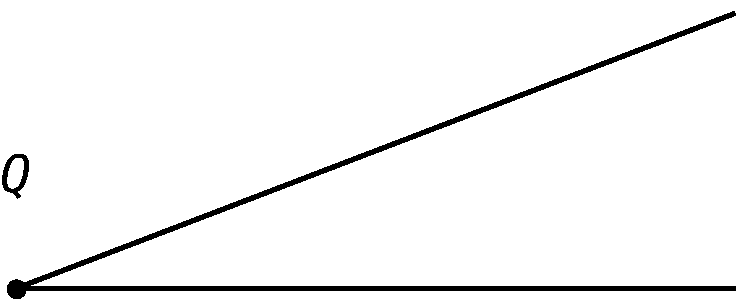
\includegraphics[width=0.33\textwidth]{fig_trans_6a}}
\hspace{1cm}
\subfigure[\label{fig_trans_6b}]{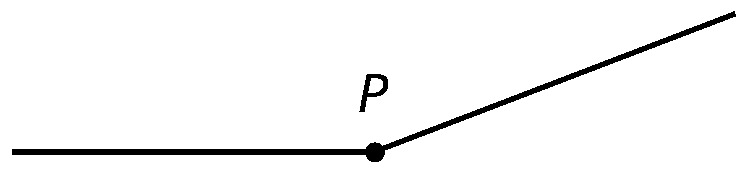
\includegraphics[width=0.33\textwidth]{fig_trans_6b}}
}
\caption{An acute angle with vertex $Q$ (a) and obtuse angle with vertrex $P$ (b). }
\label{fig_trans_6}
\end{figure}


Using our definition of the degree measure, we have that $1^{\circ}$ represents the measure of an angle which constitutes $\frac{1}{360}$ of a revolution.  Now, there are two ways to further subdivide degrees.  The first, and most familiar, is \index{decimal degrees}\index[aut]{decimale graden}\index{angle ! decimal degrees}\index[aut]{hoek ! decimale graden}\textbf{decimal degrees} (\textit{decimale graden}).  \ifvc For example, an angle with a measure of $30.5^{\circ}$ would represent a rotation halfway between $30^{\circ}$ and $31^{\circ}$, or equivalently, $\frac{30.5}{360} = \frac{61}{720}$ of a full rotation. \fi The second way to divide degrees is the \index{angle ! DMS}\index{DMS}\textbf{Degree - Minute - Second} (\textbf{DMS}) system.  In this system, one degree is divided equally into sixty minutes, and in turn, each minute is divided equally into sixty seconds.  \ifvc In symbols, we write $1^{\circ} = 60'$ and $1' = 60''$, from which it follows that  $1^{\circ} = 3600''$.  To convert a measure of $42.125^{\circ}$ to the DMS system, we start by noting that $42.125^{\circ} = 42^{\circ} + 0.125^{\circ}$. Converting the partial amount of degrees to minutes, we find $0.125^{\circ} \left( \frac{60'}{1^{\circ}} \right) = 7.5' = 7' + 0.5'$. Converting the partial amount of minutes to seconds gives  $0.5' \left(\frac{60''}{1'} \right) = 30''$.  Putting it all together yields 

\[ \begin{array}{rcl}

42.125^{\circ} & = &  42^{\circ} + 0.125^{\circ} \\
               & = & 42^{\circ} + 7.5' \\
               & = & 42^{\circ} + 7' + 0.5' \\
               & = & 42^{\circ} + 7' + 30'' \\
               & = & 42^{\circ} 7' 30''\,. \\ \end{array} \]
      
On the other hand, to convert $117^{\circ}15'45''$ to decimal degrees, we first compute $15' \left(\frac{1^{\circ}}{60'}\right) = \frac{1}{4}^{\circ}$ and $45'' \left(\frac{1^{\circ}}{3600''}\right) = \frac{1}{80}^{\circ}$. Then we find

\[ \begin{array}{rcl}

 117^{\circ}15'45'' & = & 117^{\circ} + 15' + 45'' \\ [5pt]
                    & = & 117^{\circ} + \frac{1}{4}^{\circ} + \frac{1}{80}^{\circ} \\ [5pt]
                    & = & \dfrac{9381}{80}^{\circ} \\ [5pt]
                    & = &  117.2625^{\circ}\,. \\ \end{array} \]
																				
\fi
Recall that two acute angles are called \index{complementary angles}\index{angle ! complementary}\index[aut]{hoek ! complementair}\textbf{complementary angles} (\textit{complementaire hoeken}) if their measures add to $90^{\circ}$.  Two angles, either a pair of right angles or one acute angle and one obtuse angle, are called \index{supplementary angles}\index{angle ! supplementary}\index[aut]{hoek ! supplementair}\textbf{supplementary angles} (\textit{supplementaire hoeken}) if their measures add to $180^{\circ}$. In Figure~\ref{fig_trans_7},  the angles $\alpha$ and $\beta$ are supplementary angles while the pair $\gamma$ and $\delta$ are complementary angles.



When the direction of rotation matters, we will typically use an \index{angle ! oriented}\index{oriented angle}\index[aut]{hoek ! gericht}\textbf{oriented angle} (gerichte hoek).  We imagine the angle being swept out starting from an \index{angle ! initial side}\index{initial side of an angle}\textbf{initial side} and ending at a \index{angle ! terminal side}\index{terminal side of an angle}\textbf{terminal side}. When the rotation is counter-clockwise, we say that the angle is \index{angle ! positive}\index{positive angle}\textbf{positive} (\textit{positief}); when the rotation is clockwise, we say that the angle is \index{angle ! negative}\index{negative angle}\textbf{negative} (\textit{negatief}).\index[aut]{hoek ! positief}\index[aut]{hoek ! negatief}

\begin{figure}[H]
\centering
%\raisebox{0.5cm}{
\centerline{
\subfigure[]{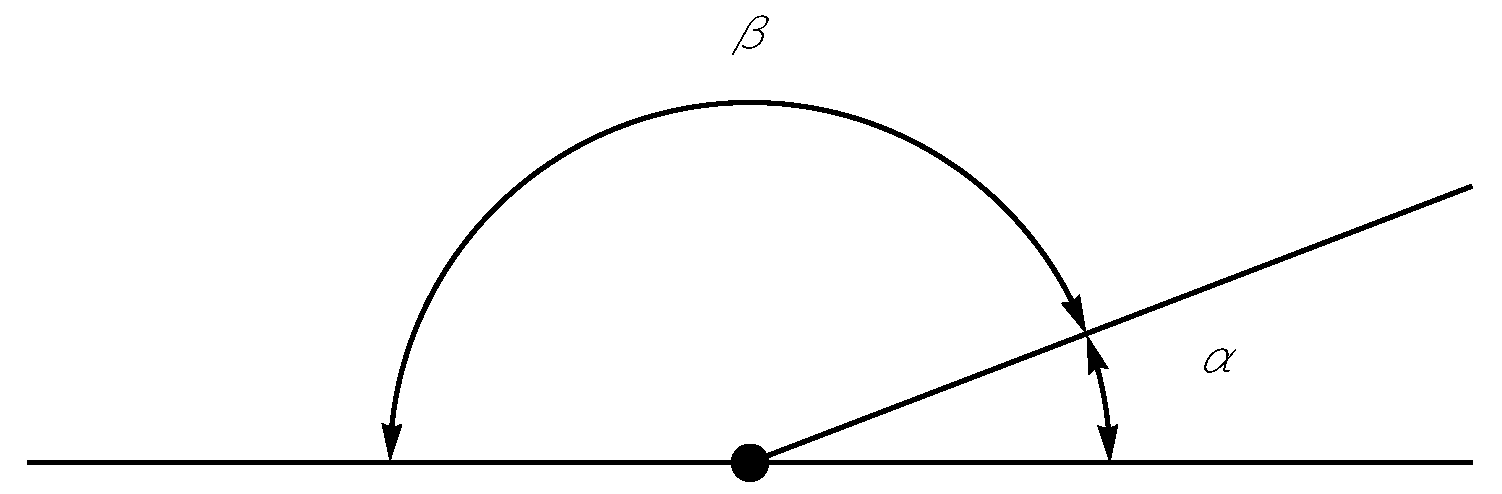
\includegraphics[width=0.5\textwidth]{fig_trans_7a}}
\hspace{1cm}
\subfigure[]{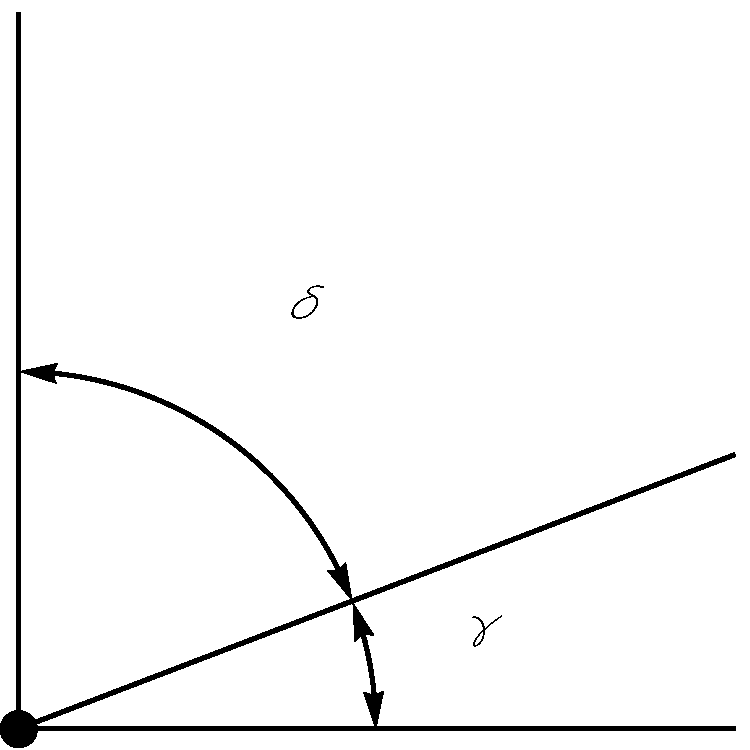
\includegraphics[width=0.25\textwidth]{fig_trans_7b}}
}
\caption{Supplementary (a) and complementary angles (b). }
\label{fig_trans_7}
\end{figure}


An angle is said to be in \index{angle ! standard position}\index{standard position of an angle}\textbf{standard position} if its vertex is the origin and its initial side coincides with the positive $x$-axis. Furthermore, two angles in standard position are called \index{angle ! coterminal}\index{coterminal angle}\textbf{coterminal} if they share the same terminal side. Such angles always differ by a multiple of $360^{\circ}$ and since there are infinitely many integers, any given angle has infinitely many coterminal angles.

Remember that the real number $\pi$ is defined to be the ratio of a circle's circumference $C$ to its diameter $d$. It is a mathematical constant. In terms of the radius, we equivalently have $2 \pi = \frac{C}{r}$. This tells us that for any circle, the ratio of its circumference to its radius is also always constant; in this case the constant is $2\pi$.  Suppose now we take a portion of the circle, so instead of comparing the entire circumference $C$ to the radius, we compare some \textbf{arc} (\textit{boog}) measuring $s$ units in length to the radius (Figure~\ref{fig_trans_8}).  Let $\theta$ be the angle whose vertex is the centre of the circle and whose determining rays pass through the endpoints of the arc.  Using proportionality arguments, it stands to reason that the ratio $\frac{s}{r}$ should also be a constant among all circles, and it is this ratio which defines the \index{angle ! radian measure}\index{radian measure}\index[aut]{hoek ! radialen}\textbf{radian measure} (\textit{radialen}) of an angle. \index{arc}  \index[aut]{boog}



\begin{figure}
	\begin{center}			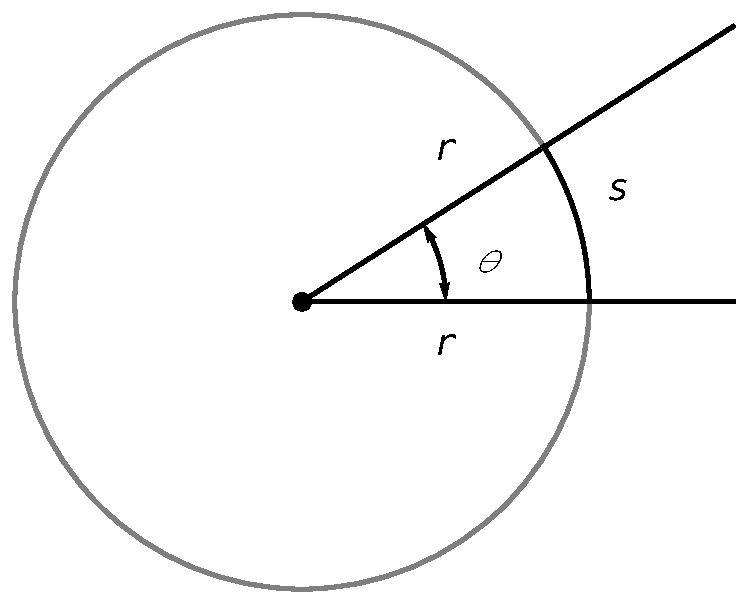
\includegraphics[width=0.4\textwidth]{fig_trans_8}
	\caption{The radian measure of $\theta$ is $\frac{s}{r}$. }
	\label{fig_trans_8}
	\end{center}
\end{figure}


We note that an angle with radian measure $1$ means the corresponding arc length $s$ equals the radius of the circle $r$, hence $s = r$.  When the radian measure is $2$, we have $s = 2r$; when the radian measure is $3$, $s = 3r$, and so forth.  Thus the radian measure of an angle $\theta$ tells us how many `radius lengths' we need to sweep out along the circle to subtend the angle $\theta$.  Since one revolution sweeps out the entire circumference $2\pi r$, one revolution has radian measure $\frac{2 \pi r}{r} = 2 \pi$.   Note that, by definition, the radian measure of an angle is a length divided by another length so that these measurements are actually dimensionless and are considered dimensionless numbers. 


Since one revolution counter-clockwise measures $360^{\circ}$ and the same angle measures $2 \pi$ radians, we can use the proportion $\frac{2 \pi \, \text{radians}}{360^{\circ}}$, or equivalently, $\frac{\pi \, \text{radians}}{180^{\circ}}$, as the conversion factor between degrees and radians.  For example, to convert $60^{\circ}$ to radians we find $ \frac{\pi}{3} \, \text{radians}$.  

The merit of the radian measure lies in how easily angles in this measure can be identified with real numbers.   Consider the unit circle,  the angle $\theta$ in standard position, and the corresponding arc measuring $s$ units in length.  By definition, and the fact that the unit circle has radius 1, the radian measure of $\theta$ is $\frac{s}{r}=\frac{s}{1} = s$ so that we have $\theta = s$.  In order to identify real numbers with oriented angles, we make good use of this fact by essentially  wrapping  the real number line around the unit circle and associating to each real number $t$ an oriented arc on the unit circle with initial point $(1,0)$.

\ifvc
\begin{example}
 Sketch the oriented arc on the unit circle corresponding to each of the following real numbers.  

\begin{multicols}{2}
\begin{enumerate}

\item $t=\dfrac{3 \pi}{4}$

\item $t =  - 2 \pi$

\end{enumerate}
\end{multicols}

\xhrulefill{gray}{2.5pt}Solution \xhrulefill{gray}{2.5pt}

\begin{enumerate}

\item  The arc associated with $t = \frac{3 \pi}{4}$ is the arc on the unit circle which subtends the angle $\frac{3 \pi}{4}$ in radian measure.  Since $\frac{3 \pi}{4}$ is $\frac{3}{8}$ of a revolution, we have an arc which begins at the point $(1,0)$ proceeds counter-clockwise up to midway through Quadrant II (Figure~\ref{fig_trans_9a}).

\item Since one revolution is $2\pi$ radians, and $t=-2\pi$ is negative, we graph  the arc which begins at $(1,0)$ and proceeds clockwise for one full revolution (Figure~\ref{fig_trans_9b}).

\end{enumerate}
\begin{figure}[H]
\centering
%\raisebox{0.5cm}{
\centerline{
\subfigure[\label{fig_trans_9a}]{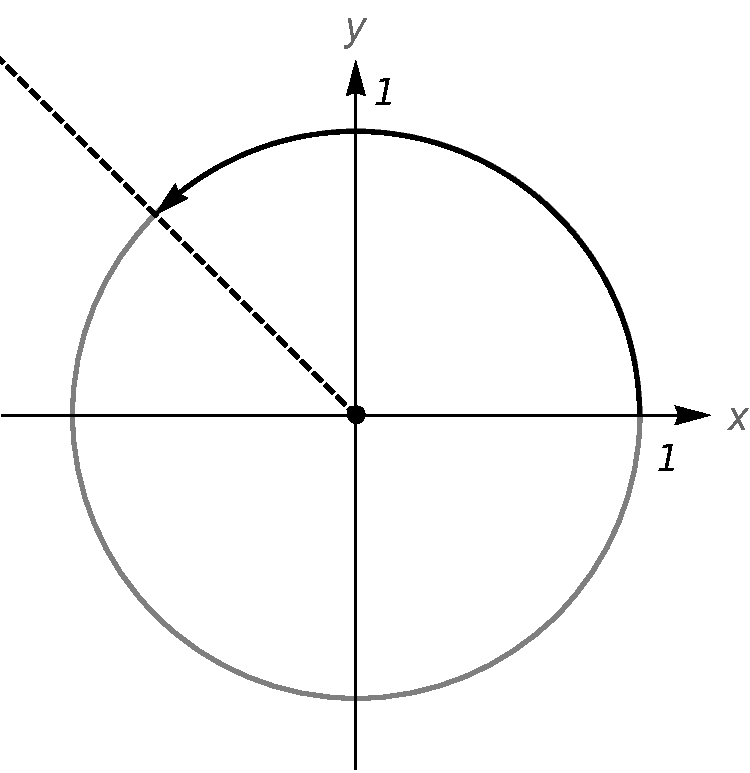
\includegraphics[width=0.43\textwidth]{fig_trans_9a}}
\hspace{0.1cm}
\subfigure[\label{fig_trans_9b}]{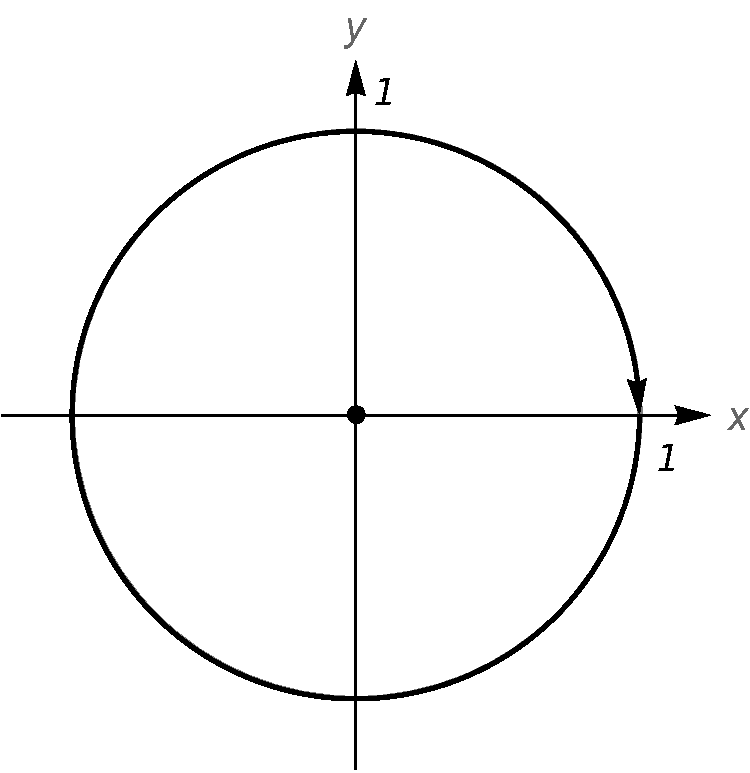
\includegraphics[width=0.43\textwidth]{fig_trans_9b}}
}
\caption{Oriented arc on the unit circle corresponding with $3\pi/4$ (a) and $-2\pi$ (b). }

\end{figure}


\end{example}
\fi
\ifcourse
\subsection{Circular motion}
Suppose an object is moving as along a circular path of radius $r$ from the point $P$ to the point $Q$ in an amount of time $t$ [T] (Figure~\ref{fig_trans_10}).  




 
Here $s$ represents a \textbf{displacement} \index{displacement} (\textit{verplaatsing}) \index[aut]{verplaatsing} so that  $s > 0$ means the object is traveling in a counter-clockwise direction and $s<0$ indicates movement in a clockwise direction. The average velocity of the object, denoted $\overline{v}$ [$T^{-1}$], is defined as the average rate of change of the position of the object with respect to time. As a result, we have $\overline{v} = \frac{s}{t}$.  The quantity $\overline{v}$ [$LT^{-1}$]  conveys two ideas: the direction in which the object is moving and how fast the position of the object is changing.  The contribution of direction in the quantity $\overline{v}$ is either to make it positive (in the case of counter-clockwise motion) or negative (in the case of clockwise motion), so that the quantity $\left| \overline{v} \right|$ quantifies how fast the object is moving - it is the speed of the object. Measuring $\theta$ in radians we have $\theta = \frac{s}{r}$ thus $s = r \theta$ and 
 \[ \overline{v} = \frac{s}{t} = \frac{r \theta}{t} = r \,\frac{\theta}{t} \,.\] 
The quantity $\frac{\theta}{t}$ is called the \index{velocity ! average angular}\index{average angular velocity}\textbf{average angular velocity} (\textit{gemiddelde hoeksnelheid}) \index[aut]{gemiddelde hoeksnelheid} of the object, denoted by $\overline{\omega}$.  The quantity $\overline{\omega}$  is the average rate of change of the angle $\theta$ with respect to time. If $\overline{\omega}$ is constant throughout the duration of the motion, then it can be shown that the average  velocities are the same as their instantaneous counterparts, $v$ and $\omega$, respectively.  In this case, $v$ is simply called the velocity of the object and is the instantaneous rate of change of the position of the object with respect to time and likewise for  $\omega$. 

If the path of the object were uncurled from a circle to form a line segment, then the velocity of the object on that line segment would be the same as the velocity on the circle.  For this reason, the quantity $v$ is often called the linear velocity of the object in order to distinguish it from the angular velocity, $\omega$. Consequently, for an object moving on a circular path of radius $r$ with constant angular velocity $\omega$, the (linear) velocity of the object is given by $v = r \omega$.  

\begin{figure}[h]
	\begin{center}
			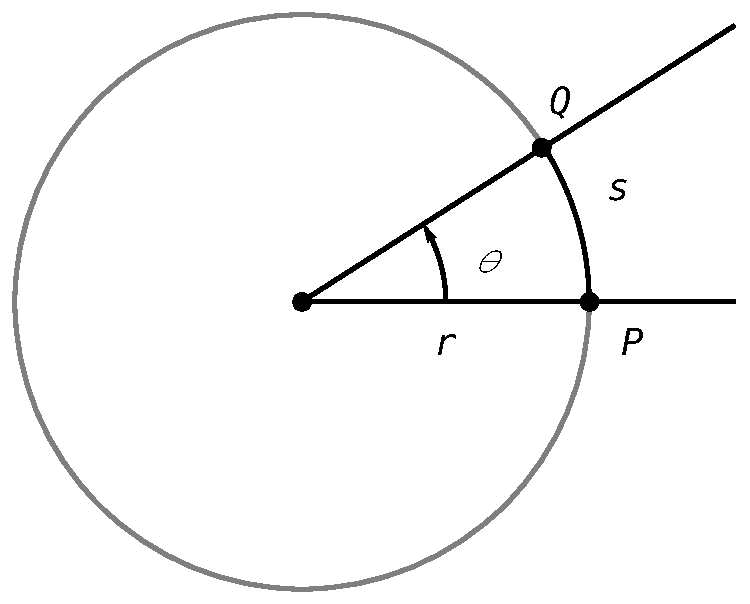
\includegraphics[width=0.4\textwidth]{fig_trans_10}
	\caption{An object  moving along a circular path of radius $r$ from $P$ to $Q$. }
	\label{fig_trans_10}
	\end{center}
\end{figure}


\begin{example}  \label{EarthRotationEx}

Assuming that the surface of the Earth is a sphere, any point on the Earth can be thought of as an object travelling on a circle which completes one revolution in (approximately) 24 hours. The path traced out by the point during this 24 hour period is the Latitude of that point.   Campus Coupure of Ghent University is at $51.05325^{\circ}$ north latitude, and the radius of the earth at this Latitude is approximately $6365$~km.  Find the linear velocity of the campus as the world turns.

\xhrulefill{gray}{2.5pt}Solution \xhrulefill{gray}{2.5pt}

 To use the formula $v = r \omega$, we first need to compute the angular velocity $\omega$.  The earth makes one revolution in 24 hours, and one revolution is $2 \pi$ radians, so $\omega = \frac{2 \pi \, \text{radians}}{24 \, \text{hours}} = \frac{\pi}{12 \, \text{hours}}$. We are also assuming that we are viewing the rotation of the earth as counter-clockwise so $\omega > 0$.  Hence, the linear velocity is \[ v = 6365 \, \text{km} \cdot \frac{\pi}{12 \, \text{h}} \approx 1666 \, \frac{\text{km}}{\text{h}}\,.\]  
\end{example}

\fi

\subsection{The six trigonometric functions}
\subsubsection{Cosine and sine on the unit circle}
The sine and cosine of an acute angle are defined in the context of a right triangle. Consider for that purpose the generic right triangle  with corresponding acute angle $\theta$ (Figure~\ref{fig_trans_11}). The side with length $a$ is called the \textbf{side of the triangle adjacent to  $\theta$} (\textit{aanliggende rechthoekzijde}); the side with length $b$ is called the \textbf{side of the triangle opposite $\theta$} (\textit{overstaande rechthoekzijde}); and the remaining side of length $c$ (the side opposite the right angle) is called the \textbf{hypotenuse} (\textit{hypothenusa})\index{hypotenuse}\index[aut]{hypothenusa}. We now imagine drawing this triangle in Quadrant I  so that the angle $\theta$ is in standard position with the adjacent side to $\theta$ lying along the positive $x$-axis (Figure~\ref{fig_trans_12}). 


\begin{figure}[H]
\centering
%\raisebox{0.5cm}{
\centerline{
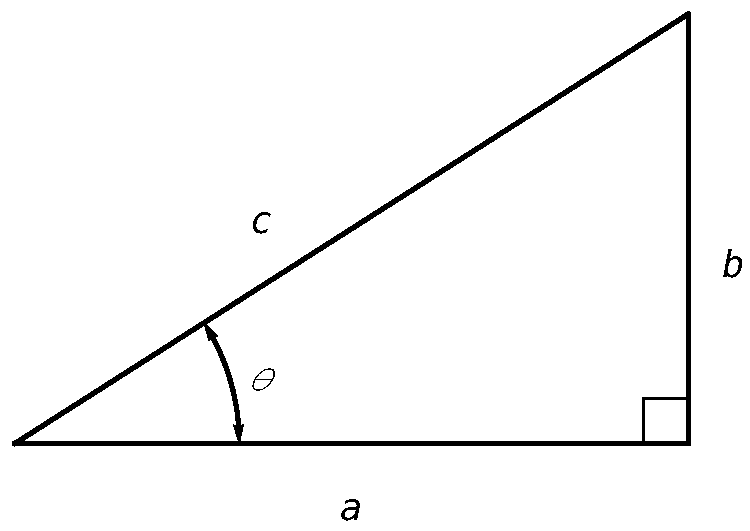
\includegraphics[width=0.3\textwidth]{fig_trans_11}}
	\caption{A right triangle with acute angle $\theta$. }
	\label{fig_trans_11}
\end{figure}

\begin{figure}[h]
	\begin{center}
			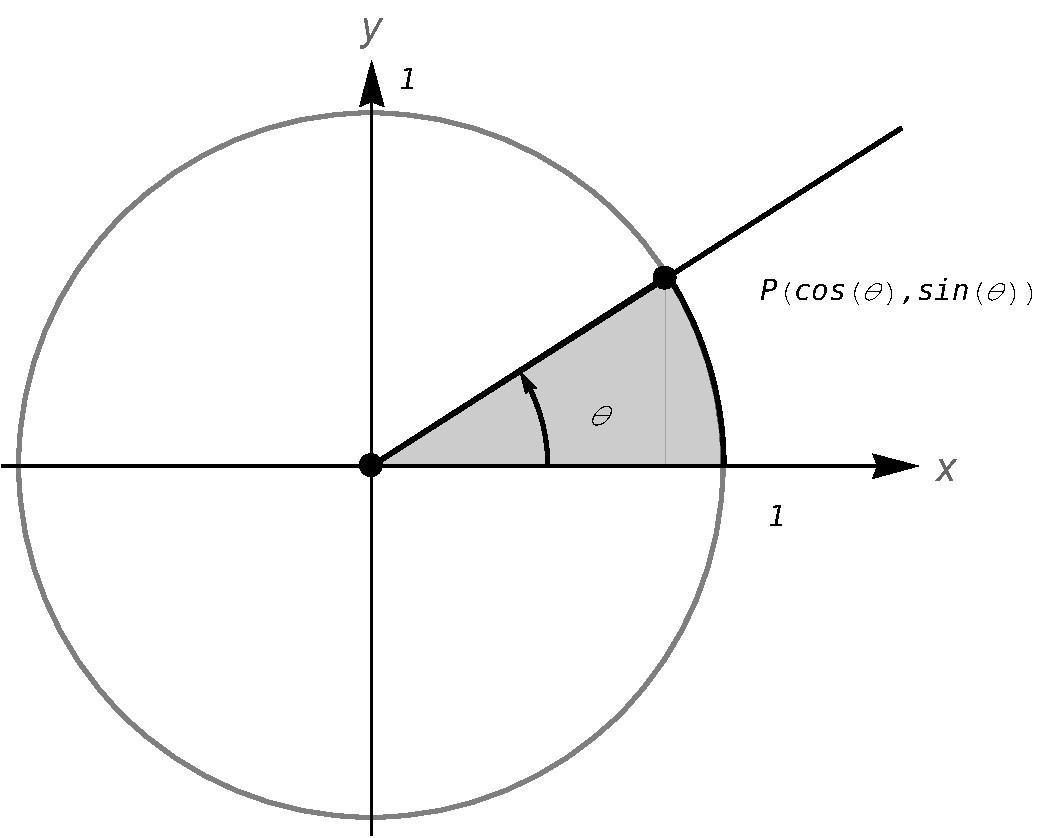
\includegraphics[width=0.5\textwidth]{fig_trans_12}
	\caption{Position of a point $P$ on the unit circle expressed in terms of $\cos(\theta)$ and $\sin(\theta)$. }
	\label{fig_trans_12}
	\end{center}
\end{figure}


Then the \index{cosine}\index[aut]{cosinus}\index[aut]{hoek ! cosinus}\textbf{cosine} (\textit{cosinus}) and \index{sine}\index[aut]{sinus}\index[aut]{hoek ! sinus}\textbf{sine} (\textit{sinus}) of $\theta$ are defined as
\begin{equation}
\cos(\theta) = \dfrac{a}{c}
\label{cosrechthoek}
\end{equation}
 and 
\begin{equation}
\sin(\theta) = \dfrac{b}{c}\,,
\label{sinrechthoek}
\end{equation}
so we have determined the cosine and sine of $\theta$ in terms of the lengths of the sides of the right triangle. 




We now imagine drawing this right triangle in Quadrant I  so that the angle $\theta$ is in standard position with the adjacent side to $\theta$ lying along the positive $x$-axis and the point $P$ lies on the unit circle (Figure~\ref{fig_trans_12}). Given Equations~\eqref{cosrechthoek} and \eqref{sinrechthoek}, we  see that the $x$-coordinate of the point $P$   is the cosine of $\theta$, while the $y$-coordinate of $P$ is the  sine of $\theta$ (Figure~\ref{fig_trans_12}).  Since, for each angle $\theta$, there is only one associated value of $\cos(\theta)$ and only one associated value of $\sin(\theta)$, both the sine and cosine may be interpreted as functions. It can be verified easily  that the gray area in Figure~\ref{fig_trans_12} equals $\theta/2$; that is halve the circular angle $\theta$. Besides, given how we defined angles, it is easy to see that $\cos(\theta)=\cos(\theta+2\,\pi)$ for all $\theta\in[0,2\pi]$, from which it follows that the cosine function is periodic with period $2\pi$. Similarly, we find that also the sine function is periodic with period $2\pi$.





Having introduced the sine and cosine, we should recall one of the most important identities in trigonometry.


\begin{theorem}[The Pythagorean identity] \label{cosinesinepythid}
For any angle $\theta$, it holds that
\begin{equation}
\cos^{2}(\theta) + \sin^{2}(\theta) = 1\,.
\label{pyth}
\end{equation}

\end{theorem}

We summarize the cosine and sine values for certain common angles in Table~\ref{tab_trans_1}. 


\begin{table}[h]
\caption{Cosine and sine value of common angles}
\label{tab_trans_1}
\renewcommand{\arraystretch}{1.75}%
\begin{tabular}{cc|cc} 
 $\theta$ (degrees) &  $\theta$ (radians) & $\cos(\theta)$ & $\sin(\theta)$ \\ \hline\hline
$0^{\circ}$ & 0 & 1 & 0 \\
$30^{\circ}$ & $\dfrac{\pi}{6}$ & $\dfrac{\sqrt{3}}{2}$ & $\dfrac{1}{2}$ \\[0.2cm] 
$45^{\circ}$ & $\dfrac{\pi}{4}$ & $\dfrac{\sqrt{2}}{2}$ & $\dfrac{\sqrt{2}}{2}$ \\[0.2cm] 
$60^{\circ}$ & $\dfrac{\pi}{3}$ & $\dfrac{1}{2}$ & $\dfrac{\sqrt{3}}{2}$ \\[0.2cm] 
$90^{\circ}$ & $\dfrac{\pi}{2}$ & 0 & 1 \\ [2pt] 
\renewcommand{\arraystretch}{1}%
\end{tabular}
\end{table}


To determine the cosines and sines of angles not given in Table~\ref{tab_trans_1} we may exploit the symmetry inherent in the unit circle.  Suppose, for instance, we wish to know the cosine and sine of  $\theta = 5 \pi/6$. We plot $\theta$ in standard position below and, as usual, let $P(x,y)$ denote the point on the terminal side of $\theta$ which lies on the unit circle.  Note that the terminal side of $\theta$ lies $\pi/6$ radians short of one half revolution (Figure~\ref{fig_trans_13b}).  Knowing from Table~\ref{tab_trans_1} that $\cos\left(\frac{\pi}{6}\right) = \frac{\sqrt{3}}{2}$ and $\sin\left( \frac{\pi}{6} \right) = \frac{1}{2}$.   This means that the point on the terminal side of the angle $\frac{\pi}{6}$, when plotted in standard position, is $\left(\frac{\sqrt{3}}{2}, \frac{1}{2}\right)$.  From Figure~\ref{fig_trans_13b}, it is clear that the point $P(x,y)$ we seek can be obtained by reflecting that point about the $y$-axis.  Hence,  $\cos\left(\frac{5\pi}{6}\right) = -\frac{\sqrt{3}}{2}$ and $\sin\left( \frac{5\pi}{6} \right) = \frac{1}{2}$. 


\begin{figure}[h]
\centering
%\raisebox{0.5cm}{
\centerline{
\subfigure[\label{fig_trans_13a}]{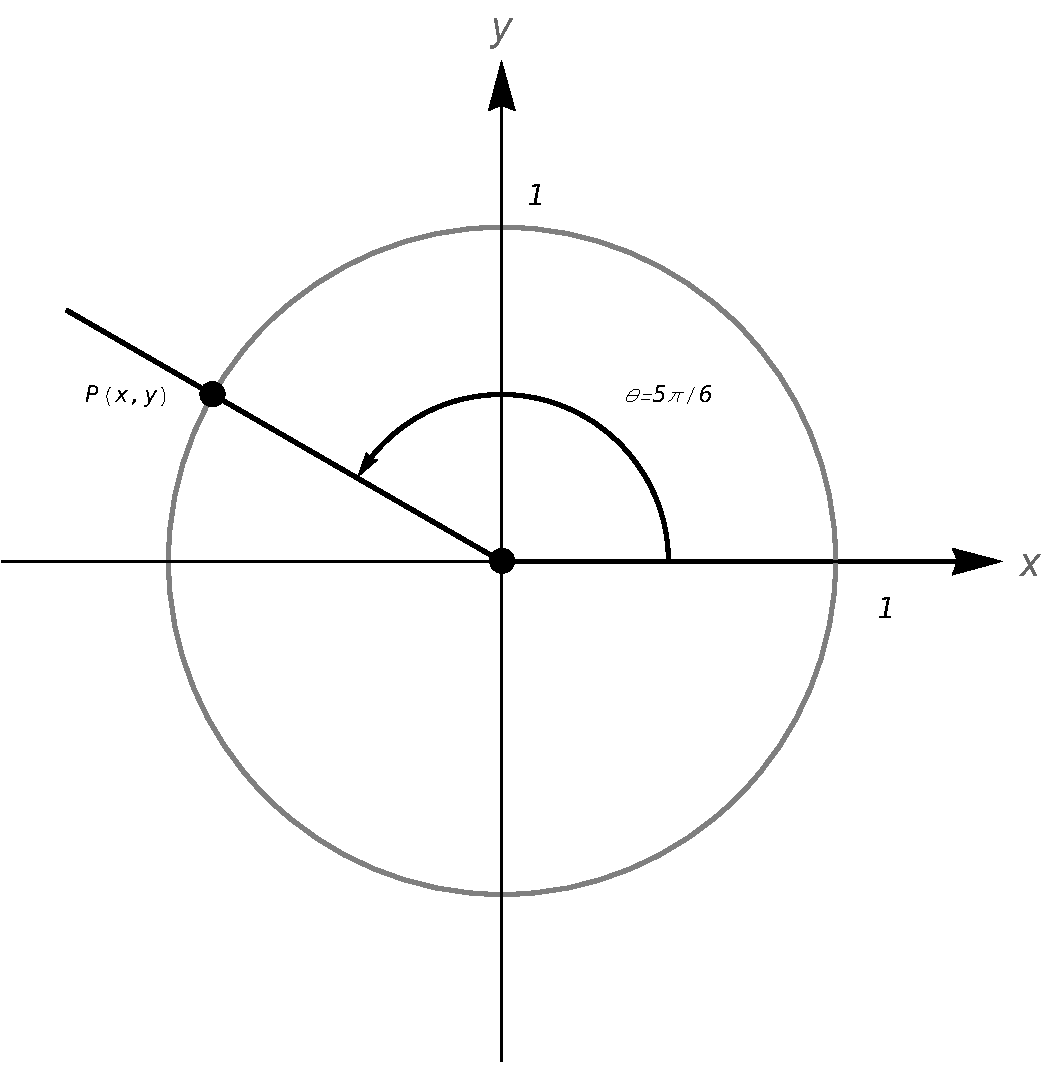
\includegraphics[width=0.45\textwidth]{fig_trans_13a}}
\hspace{0.1cm}
\subfigure[\label{fig_trans_13b}]{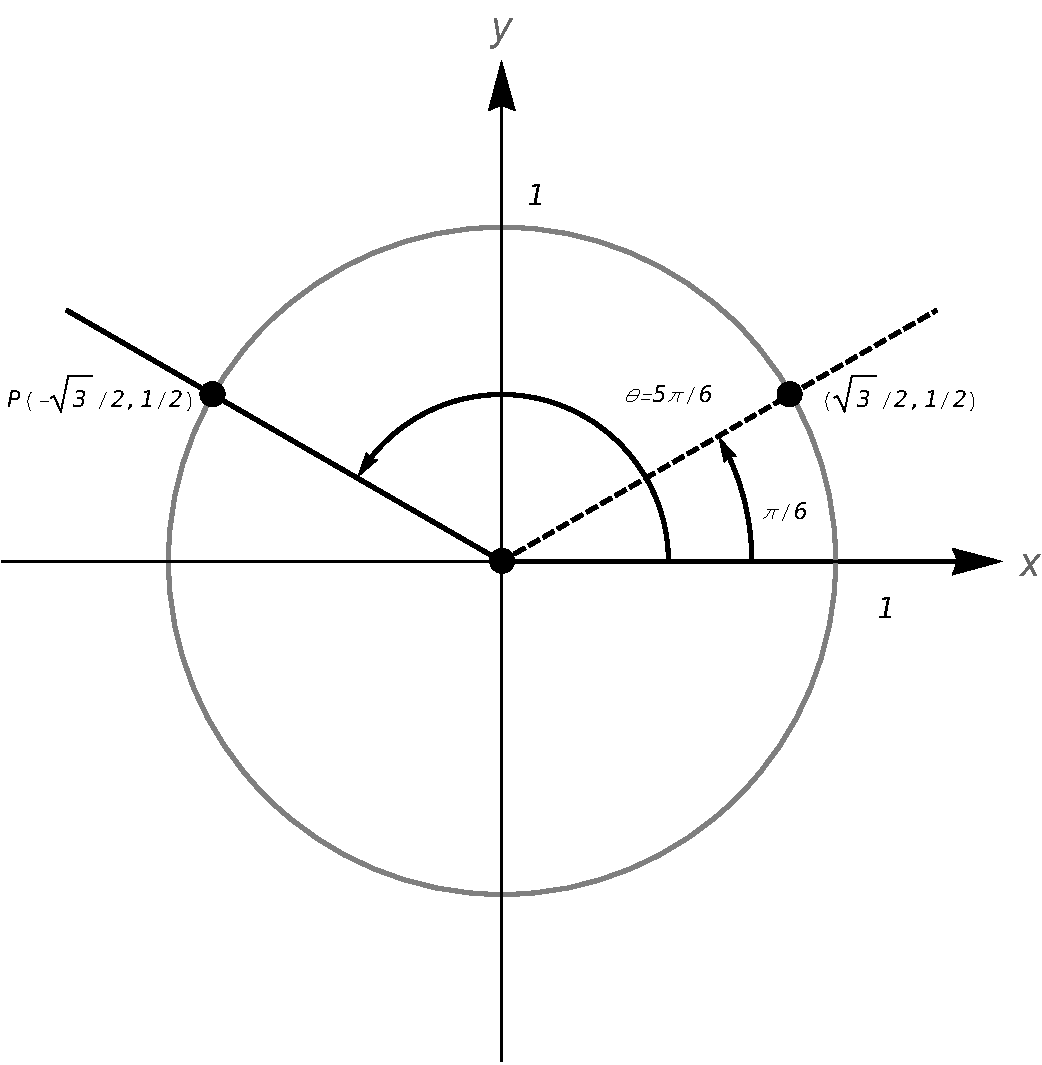
\includegraphics[width=0.45\textwidth]{fig_trans_13b}}
}
\caption{Determining the $\cos\left(\frac{5\pi}{6}\right)$ and  $\sin\left(\frac{5\pi}{6}\right)$. }

\end{figure}

\ifvc

\begin{example}
 Find the cosine and sine of the following angles, provided $\alpha\in]0,\frac{\pi}{2}[$.

\begin{multicols}{2}

\begin{enumerate}

\item  $\theta = \dfrac{11 \pi}{6}$

\item  $\theta = -\dfrac{5 \pi}{4}$

\item  $\theta = \pi+\alpha$

\item $\theta=2\pi-\alpha$

\end{enumerate}

\end{multicols}
\pagebreak
\xhrulefill{gray}{2.5pt}Solution \xhrulefill{gray}{2.5pt}

\begin{enumerate}

\item The terminal side of  $\theta = \frac{11\pi}{6}$, when plotted in standard position, lies in Quadrant IV, just $\frac{\pi}{6}$ radians short of the positive $x$-axis.  Since we know from Table~\ref{tab_trans_1} that $\cos\left(\frac{\pi}{6}\right)=\frac{\sqrt{3}}{2}$ and $\sin\left(\frac{\pi}{6}\right) =  \frac{1}{2}$, we easily find using the symmetry inherent in the unit circle that $\cos\left(\frac{11 \pi}{6} \right) = \cos\left(\frac{\pi}{6} \right) = \frac{\sqrt{3}}{2}$ and $\sin\left(\frac{11\pi}{6}\right) = -\sin\left(\frac{\pi}{6}\right) =  -\frac{1}{2}$ (Figure~\ref{fig_trans_14a}).

\item  To plot $\theta = -\frac{5\pi}{4}$, we rotate clockwise an angle of $\frac{5 \pi}{4}$ from the positive $x$-axis.  The terminal side of $\theta$, therefore, lies in Quadrant~II making an angle of $\alpha = \frac{5 \pi}{4} - \pi = \frac{\pi}{4}$ radians with respect to the negative $x$-axis.   Since  we know from Table~\ref{tab_trans_1} that $\cos\left(\frac{\pi}{4}\right) = \frac{\sqrt{2}}{2}$ and $\sin\left(\frac{\pi}{4}\right) = \frac{\sqrt{2}}{2}$, we easily find using the symmetry inherent in the unit circle that   $\cos\left(-\frac{5 \pi}{4}\right) = -\cos\left(\frac{\pi}{4}\right) = -\frac{\sqrt{2}}{2}$ and $\sin\left(-\frac{5 \pi}{4}\right) = \sin\left(\frac{\pi}{4}\right) = \frac{\sqrt{2}}{2}$ (Figure~\ref{fig_trans_14b}).

\item  To find the cosine and sine of $\theta = \pi + \alpha$, we first plot $\theta$ in standard position. We can imagine the sum of the angles $\pi + \alpha$ as a sequence of two rotations: a rotation of $\pi$ radians followed by a rotation of  $\alpha$ radians. Since $\alpha$ is an acute angle, the terminal side of $\theta$ lies in Quadrant III, so we get through the symmetry inherent in the unit circle that $\cos(\theta) = - \cos(\alpha)$ and $\sin(\theta) = -\sin(\alpha)$ (Figure~\ref{fig_trans_14c}).


\item  Rewriting $\theta = 2\pi - \alpha$ as $\theta = 2\pi + (-\alpha)$, we can  plot $\theta$ by visualizing one complete revolution counter-clockwise followed by a clockwise  revolution  of $\alpha$ radians.  Since $\alpha$ is an acute angle, the terminal side of $\theta$ lies in Quadrant II, so we get through the symmetry inherent in the unit circle that  $\cos(\theta) =  \cos(\alpha)$ and $\sin(\theta) = -\sin(\alpha)$ (Figure~\ref{fig_trans_14d}).



\end{enumerate}

\begin{figure}[H]
\centering
%\raisebox{0.5cm}{
\centerline{
\subfigure[\label{fig_trans_14a}]{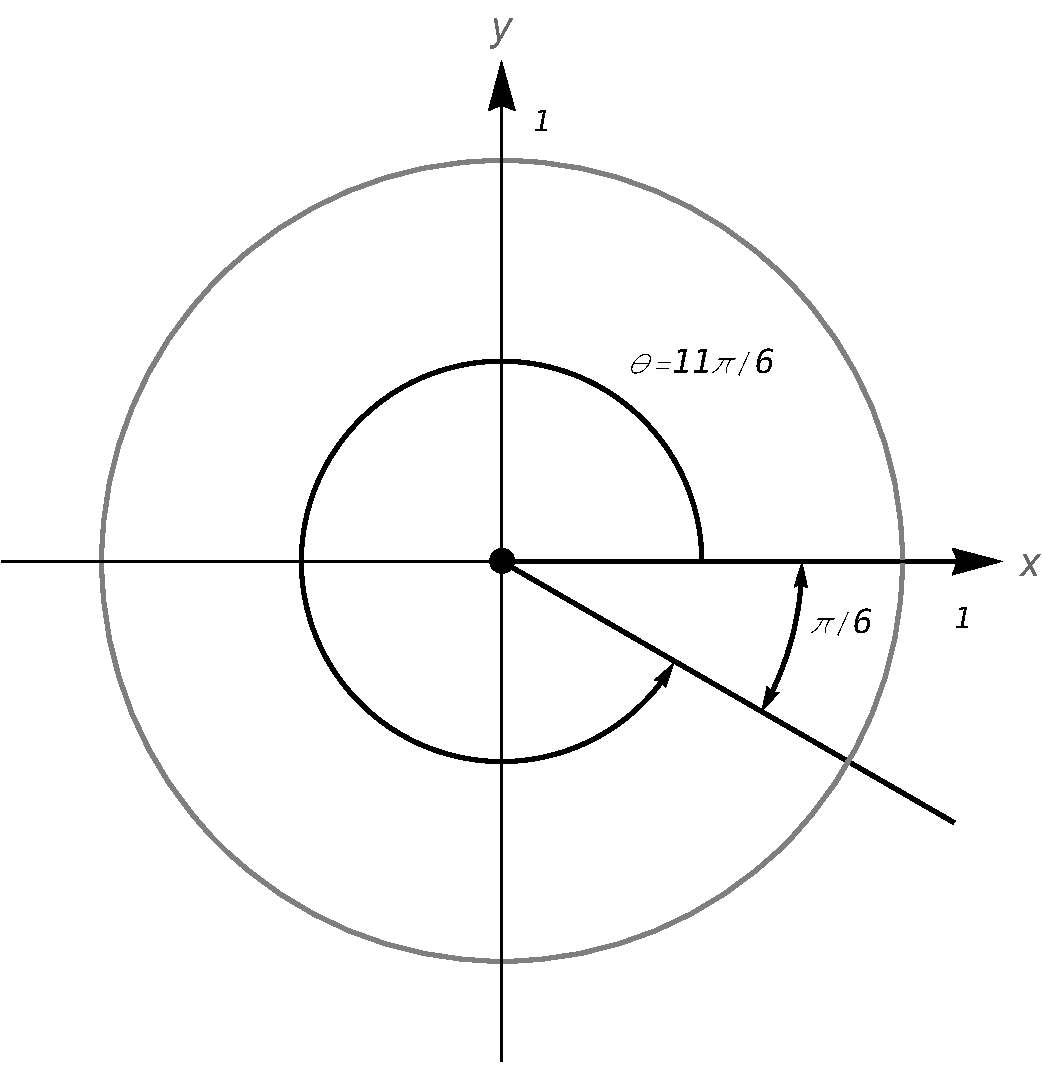
\includegraphics[width=0.43\textwidth]{fig_trans_14a}}
\hspace{0.1cm}
\subfigure[\label{fig_trans_14b}]{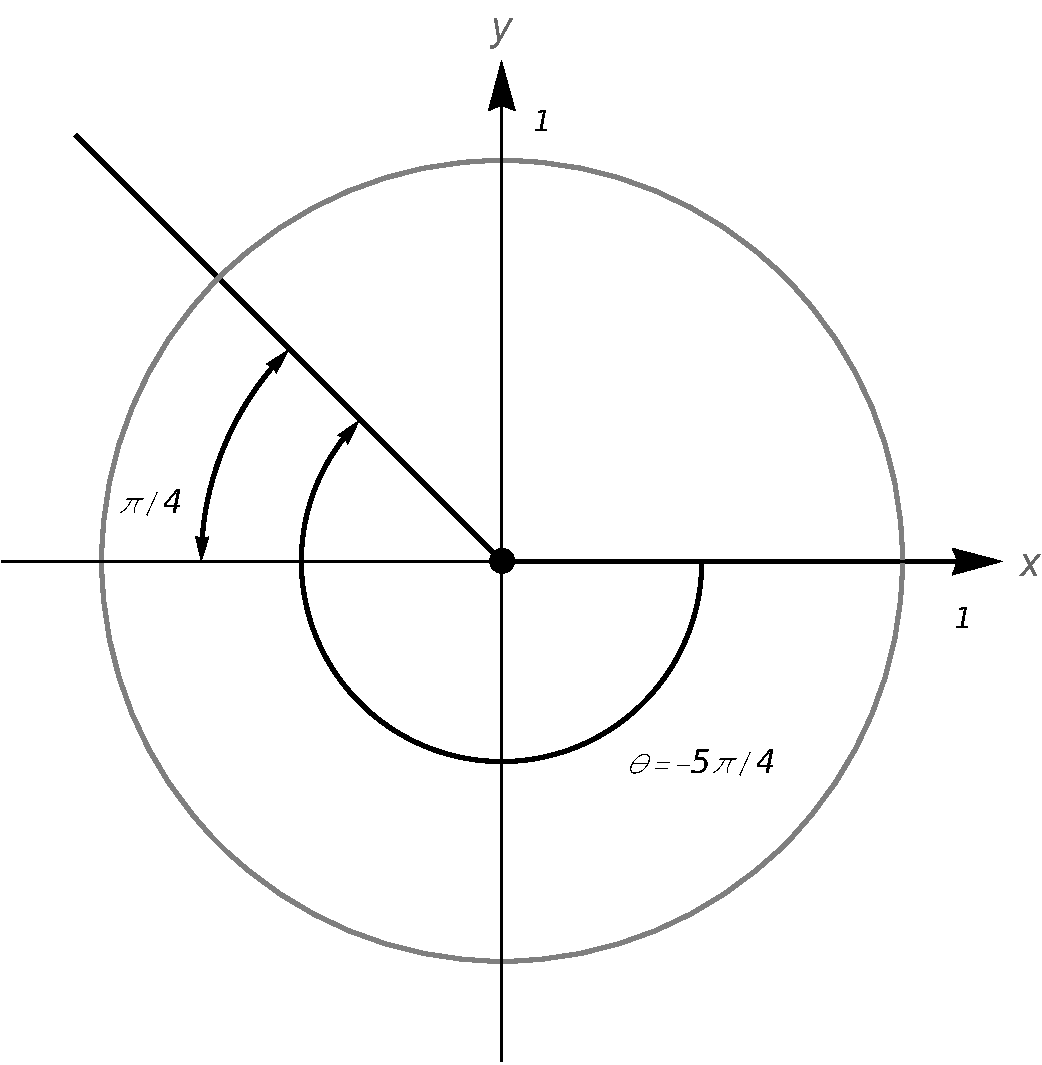
\includegraphics[width=0.43\textwidth]{fig_trans_14b}}
}
\centerline{
\subfigure[\label{fig_trans_14c}]{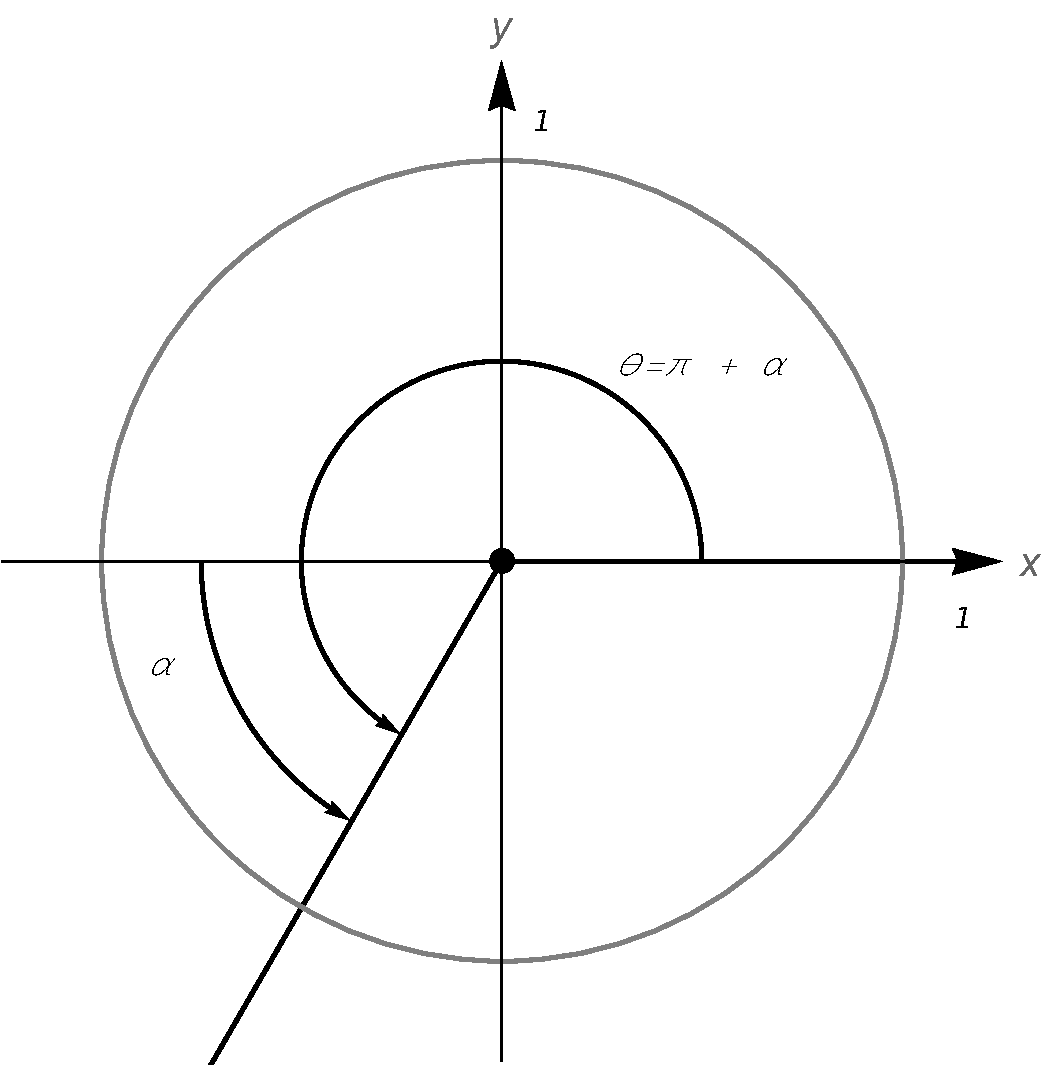
\includegraphics[width=0.43\textwidth]{fig_trans_14c}}
\hspace{0.1cm}
\subfigure[\label{fig_trans_14d}]{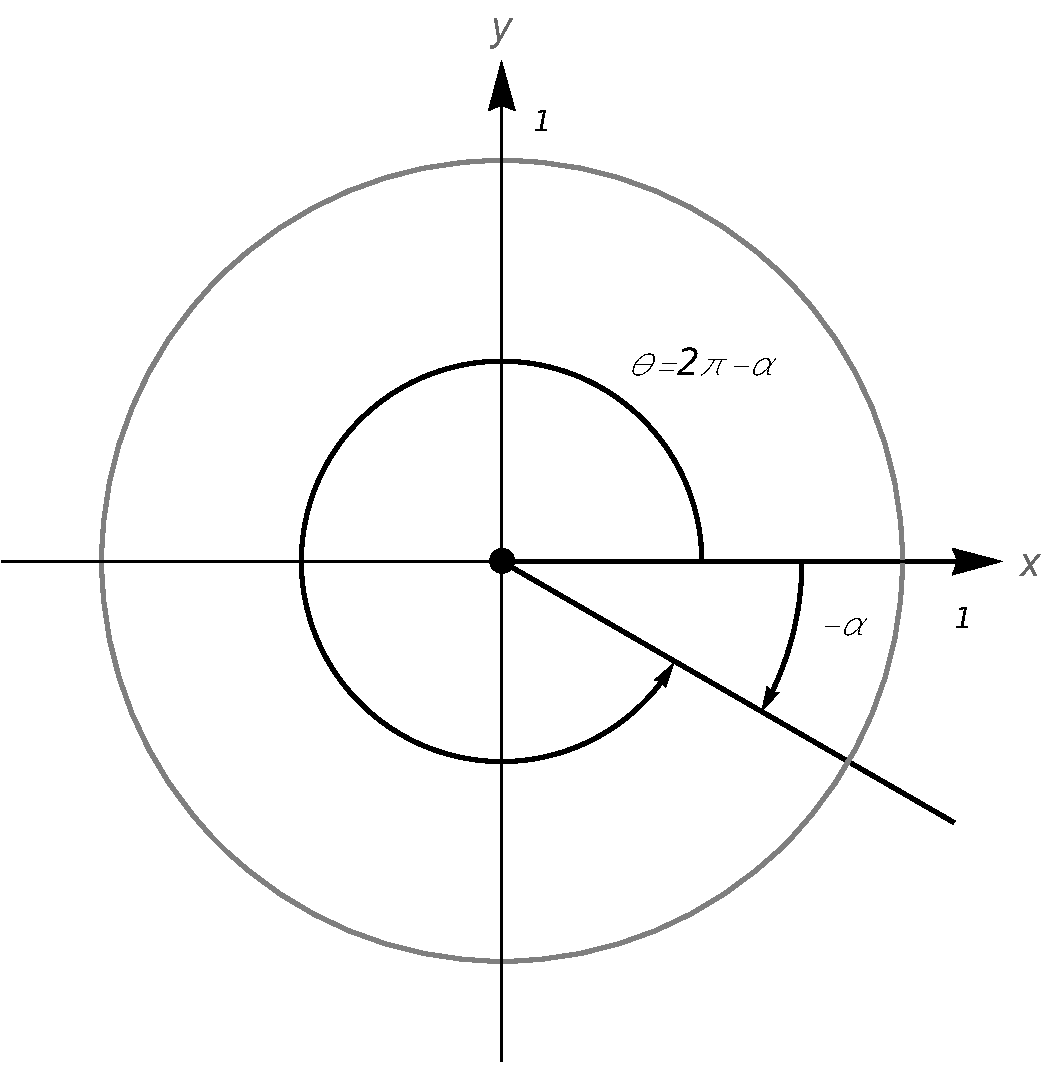
\includegraphics[width=0.43\textwidth]{fig_trans_14d}}
}
\caption{Finding the cosine and sine of $\frac{11\pi}{6}$ (a), $-\frac{5\pi}{4}$ (b),  $\pi+\alpha$ (c) and $2\pi-\alpha$ (d). }

\end{figure}
\end{example}

\fi

\subsubsection{Beyond the unit circle}
In defining the cosine and sine functions, we assigned to each angle a position on the unit circle.  Here, we broaden our scope to include circles of radius $r$ centred at the origin.  Consider for the moment the acute angle $\theta$ drawn in Figure~\ref{fig_trans_15} in standard position. Let $Q(x,y)$ be the point on the terminal side of $\theta$ which lies on the circle $x^2+y^2 = r^2$, and let $P(\widetilde{x},\widetilde{y})$ be the point on the terminal side of $\theta$ which lies on the unit circle.   Now consider dropping perpendiculars from $P$ and $Q$ to create two right triangles, $\Delta OPA$ and $\Delta OQB$. These triangles are \textbf{similar} (\textit{gelijkvormig}) \index{similar} \index[aut]{gelijkvormig}, thus it follows that $\frac{x}{\widetilde{x}} = \frac{r}{1} = r$, so $x = r \widetilde{x}$ and, similarly, we find $y = r \widetilde{y}$.  Since, by definition, $\widetilde{x} = \cos(\theta)$ and $\widetilde{y} = \sin(\theta)$,  we get the coordinates of $Q$ to be $x = r \cos(\theta)$ and $y = r \sin(\theta)$.  By reflecting these points through the $x$-axis, $y$-axis and origin, we obtain the result for all other angles $\theta$.

\begin{figure}
	\begin{center}
			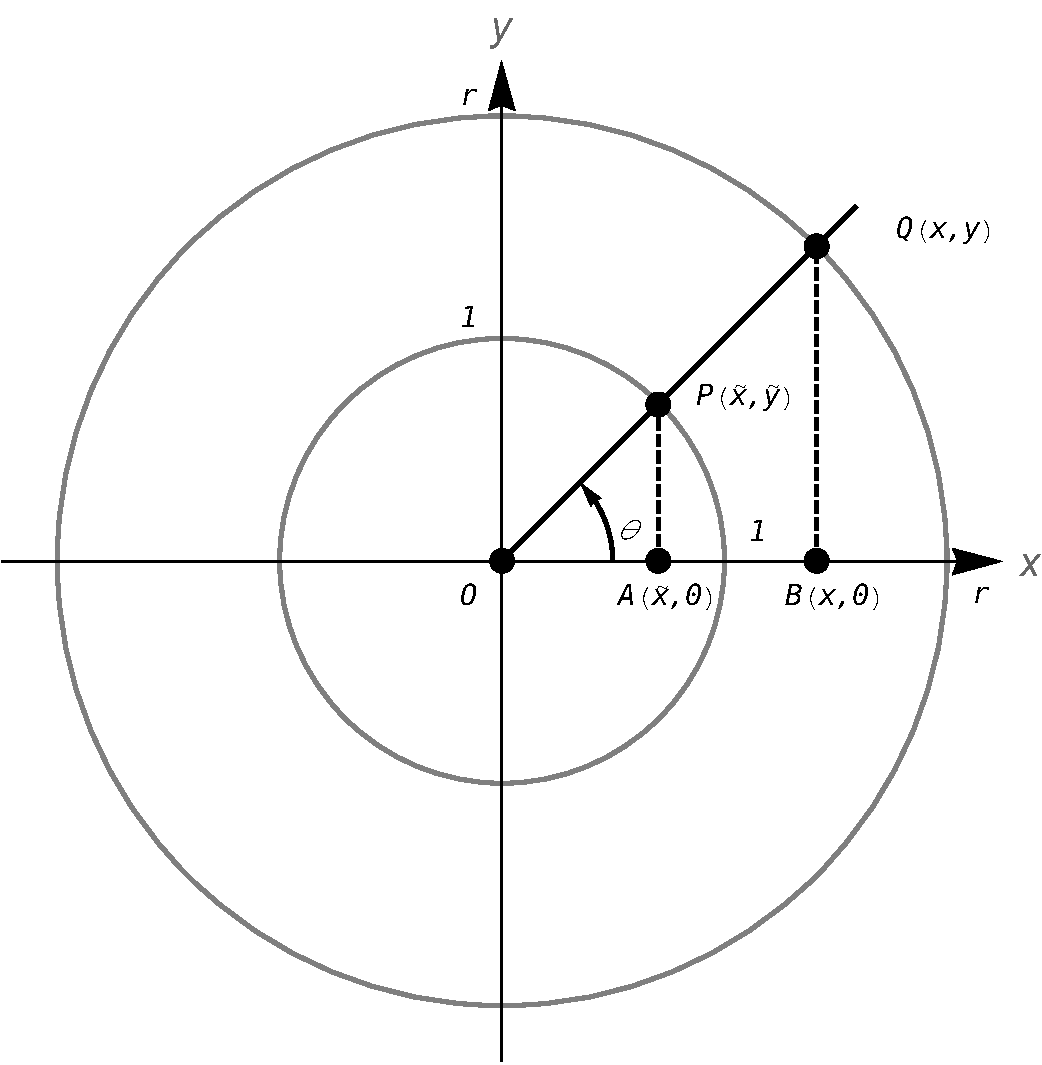
\includegraphics[width=0.45\textwidth]{fig_trans_15}
	\caption{Relation between the coordinates of a point $P$ on the unit circle and a point $Q$ on the circle $x^2+y^2 = r^2$, where both $P$ and $Q$ lie on the terminal side of $\theta$. }
	\label{fig_trans_15}
	\end{center}
\end{figure}

\pagebreak
The result is summarized in the following theorem.

\begin{theorem}[Sine and cosine in the unit circle]  \label{cosinesinecircle} 
If $Q(x,y)$ is the point on the terminal side of an angle $\theta$, plotted in standard position, which lies on the circle $x^2+y^2 = r^2$ then $x = r \cos(\theta)$ and $y = r \sin(\theta)$.  Moreover, \index{cosine} \index{sine}\index[aut]{cosinus} \index[aut]{sinus}

\[\begin{array}{ccc} \cos(\theta)= \dfrac{x}{r}  = \dfrac{x}{\sqrt{x^2+y^2}} & \text{and} &  \sin(\theta) = \dfrac{y}{r} = \dfrac{y}{\sqrt{x^2+y^2}}\,. \\ \end{array} \]

\end{theorem}
\ifanalysis
\begin{proof}
See above.
\end{proof}
\fi


Theorem \ref{cosinesinecircle} also gives us what we need to describe the position of an object travelling in a circular path of radius $r$ with constant angular velocity $\omega$.  Suppose that at time $t$, the object has swept out an angle measuring $\theta$ radians.  If we assume that the object is at the point $(r,0)$ when $t=0$, the angle $\theta$ is in standard position.  By definition, $\omega = \frac{\theta}{t}$ which we rewrite as  $\theta = \omega t$.  According to Theorem \ref{cosinesinecircle}, the location of the object $Q(x,y)$ on the circle is found using the equations  $x = r \cos(\theta) = r \cos(\omega t)$ and $y = r \sin(\theta) = r \sin(\omega t)$.  Hence, at time $t$, the object is at the point $(r \cos(\omega t), r \sin(\omega t))$, where  $\omega > 0$ indicates a counter-clockwise direction and $\omega < 0$ indicates a clockwise direction.

\ifcourse
\begin{example}
 Suppose we are in the situation of Example \ref{EarthRotationEx}.  Find the equations of motion of Campus Coupure as the earth rotates.
\label{Lakelandrotates}

\xhrulefill{gray}{2.5pt}Solution \xhrulefill{gray}{2.5pt}

  From Example \ref{EarthRotationEx}, we take $r = 6365$ km and and $\omega = \frac{\pi}{12 \, \text{hours}}$.  Hence, the equations of motion are $x =  r \cos(\omega t) = 6365 \cos\left(\frac{\pi}{12} t\right)$ and  $y =  r \sin(\omega t) = 6365 \sin\left(\frac{\pi}{12} t\right)$, where $x$ and $y$ are measured in km and $t$ is measured in hours. 
\end{example}

\fi


\subsubsection{The other trigonometric functions}
Starting from the sine and cosine functions we introduced earlier,
we may define four more trigonometric functions, being the \index{secant}\index[aut]{secans}\textbf{secant} (\textit{secans}) of $x$:
$$\sec(x) = \dfrac{1}{\cos(x)}\,,\qquad \text{provided} \cos(x) \neq 0\,, $$
the \index{cosecant}\index[aut]{cosecans}\textbf{cosecant} (\textit{cosecans}) of $x$:
$$\csc(x) = \dfrac{1}{\sin(x)}\,,\qquad \text{provided}  \sin(x) \neq 0\,,$$
the \index{tangent}\index[aut]{tangens}\textbf{tangent} (\textit{tangens}) of $x$:
$$\tan(x) = \dfrac{\sin(x)}{\cos(x)}\,,\qquad \text{provided} \cos(x) \neq 0 \,,$$
  and finally  the \index{cotangent}\index[aut]{cotangens}\textbf{cotangent} (\textit{cotangens}) of $x$:
$$\cot(x) = \dfrac{\cos(x)}{\sin(x)}\,,\qquad \text{provided} \sin(x) \neq 0\,.$$


Note that of the six trigonometric functions, only cosine and sine are defined for all angles. Table~\ref{tab_trans_2} lists the tangent and cotangent for certain common angles. 

\begin{table}[H]
\caption{Tangent and cotangent of common angles}
\label{tab_trans_2}
\renewcommand{\arraystretch}{1.75}%
\begin{tabular}{cc|cc} 
 $x$ (degrees) &  $x$ (radians) & $\tan(x)$ & $\cot(x)$ \\ \hline\hline
$0^{\circ}$ & 0 & 0 & undefined \\ 
$30^{\circ}$ & $\dfrac{\pi}{6}$ & $\dfrac{\sqrt{3}}{3}$ & $\sqrt{3}$ \\ [2pt] 
$45^{\circ}$ & $\dfrac{\pi}{4}$ & 1 & 1\\ [2pt] 
$60^{\circ}$ & $\dfrac{\pi}{3}$ & $\sqrt{3}$& $\dfrac{\sqrt{3}}{3}$ \\ [2pt] 
$90^{\circ}$ & $\dfrac{\pi}{2}$ & undefined & 0 \\ [2pt] 
\end{tabular}
\renewcommand{\arraystretch}{1}%
\end{table}


\ifvc
\begin{example}  \label{solveforangle2}  

Find all angles which satisfy the given equation.   

\begin{multicols}{3}

\begin{enumerate}

\item  $\sec(x) =2$

\item  $\tan(x) = \sqrt{3}$

\item  \label{cotangentisnegativeone} $\cot(x) = -1$.

\end{enumerate}

\end{multicols}


\xhrulefill{gray}{2.5pt}Solution \xhrulefill{gray}{2.5pt}

\begin{enumerate}

\item  We first convert to cosines and get $\frac{1}{\cos(x)} = 2$ or $\cos(x) = \frac{1}{2}$. If $\cos(x) = \frac{1}{2}$, then the terminal side of $x$, when plotted in standard position, intersects the unit circle at $x=\frac{1}{2}$. A first obvious angle $x$ for which this holds is $\frac{\pi}{3}$, so when accounting for the periodicity of the cosine we find $x=\frac{\pi}{3}+2\pi\,k$ for $k\in\mathbb{Z}$. A second angle $x$ for which the studied equation holds is $\frac{5\pi}{3}$, such that  $x = \frac{5\pi}{3} + 2\pi k$ for integers $k$ are also solutions (Figure~\ref{fig_trans_16}).


\begin{figure}[H]
	\begin{center}
			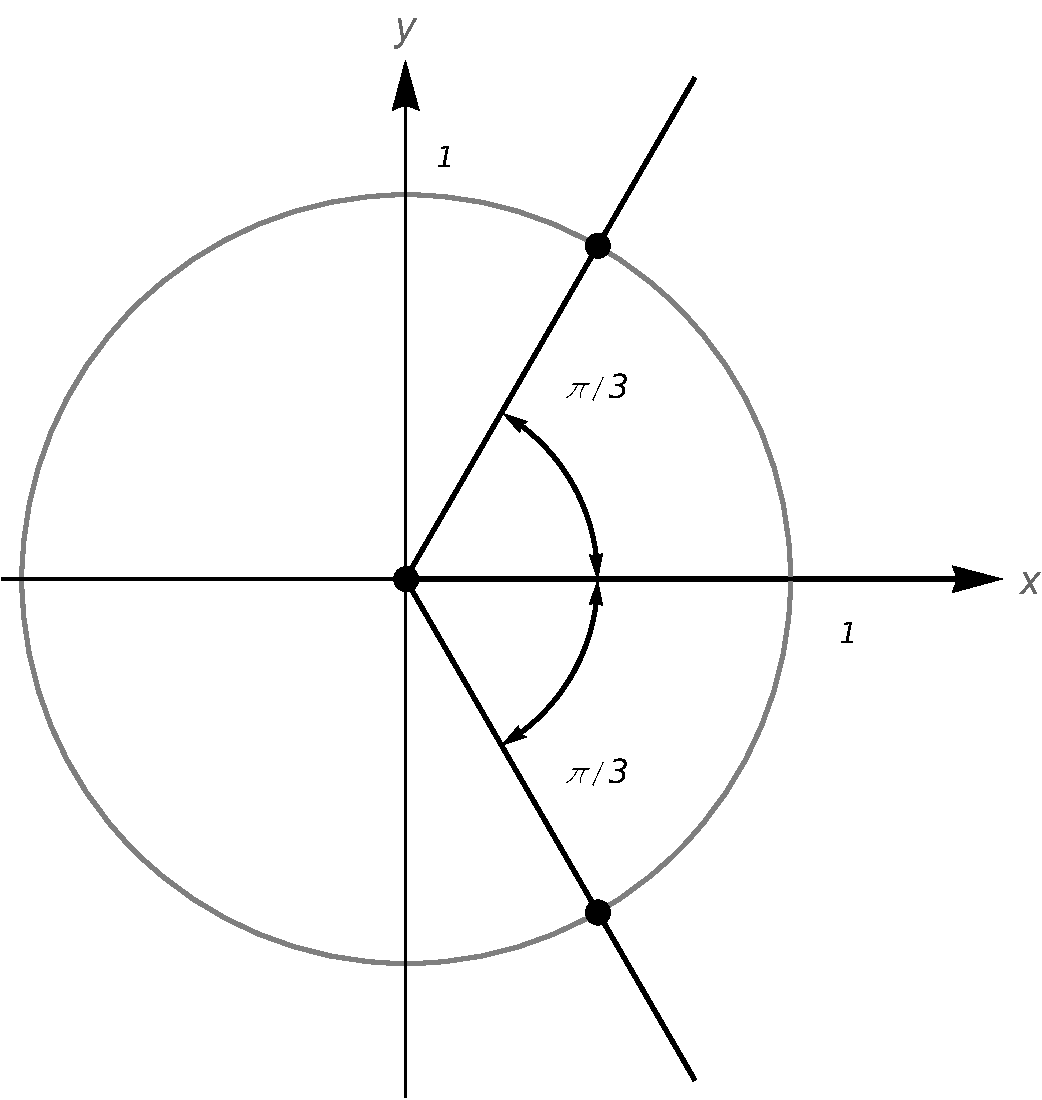
\includegraphics[width=0.4\textwidth]{fig_trans_16}
	\caption{Solving $\sec(x)=2$. }
	\label{fig_trans_16}
	\end{center}
\end{figure}


\item From Table~\ref{tab_trans_2}, we see  $\tan\left(\frac{\pi}{3}\right) = \sqrt{3}$. Hence, we  know  that the solutions to $\tan(x) = \sqrt{3}$ must, therefore, have a reference angle of $\frac{\pi}{3}$. Since the tangent is positive when $\sin(x)$ and $\cos(x)$ have the same sign, which happens in Quadrants I and III.  In Quadrant I, we get the solutions: $x = \frac{\pi}{3} + 2\pi k$ for integers $k$, and for Quadrant III, we get $x = \frac{4\pi}{3} + 2\pi k$ for integers $k$. These descriptions can be combined as $x = \frac{\pi}{3} + \pi k$ for integers $k$. 
  

\item  From Table~\ref{tab_trans_2}, we see that $\frac{\pi}{4}$ has a cotangent of $1$, which means the solutions to $\cot(x) = -1$ have a reference angle of $\frac{\pi}{4}$. If $\cot(x)$ is negative, then $\cos(x)$ and $\sin(x)$ must have different signs, so our solutions lie in Quadrants II and IV.  Our Quadrant II solution is $x = \frac{3\pi}{4} + 2\pi k$, and for Quadrant IV, we get $x = \frac{7\pi}{4} + 2\pi k$ for integers $k$.  These lists can be combined as  $x = \frac{3\pi}{4} + \pi k$ for integers $k$.
\end{enumerate}



\end{example}
\fi


 By combining Equations~\eqref{cosrechthoek} and \eqref{sinrechthoek} with the definition of the four other trigonometric functions, we can also express these in terms of the sides of a right triangle
$$
\begin{array}{llll}  \sec(\theta) = \dfrac{c}{a}\,, \;\;\;\;\;\; & \csc(\theta) = \dfrac{c}{b}\,, \;\;\;\;\;\; & \tan(\theta) = \dfrac{b}{a}\,, \;\;\;\;\;\; & \cot(\theta) = \dfrac{a}{b}\,,  \end{array}
$$
where $a$, $b$ and $c$ are defined as in Figure~\ref{fig_trans_11}. 

\ifcourse
\begin{example}
\label{exmaple}
In order to determine the height of the maple tree (\textit{Acer pseudoplatanus}) in the inner yard of Campus Coupure, two sightings from the ground, one 20 metres directly behind the other, are made.  If the angles of inclination were $45^{\circ}$ and $30^{\circ}$, respectively, how tall is the tree to the nearest foot?

\xhrulefill{gray}{2.5pt}Solution \xhrulefill{gray}{2.5pt}

Sketching the problem situation in Figure~\ref{fig_trans_17}, we find ourselves with two unknowns: the height $h$ of the tree and the distance $x$ from the base of the tree to the first observation point. 

\begin{figure}[H]
	\begin{center}
			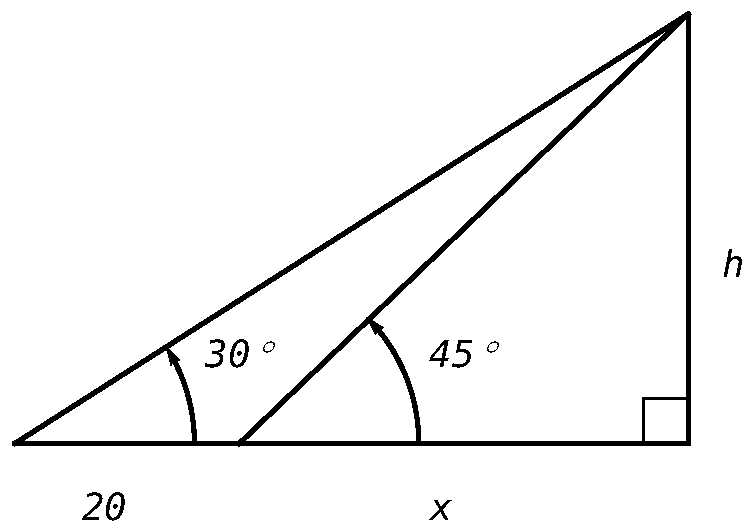
\includegraphics[width=0.4\textwidth]{fig_trans_17}
	\caption{Determining the height of a maple tree. }
	\label{fig_trans_17}
	\end{center}
\end{figure}

Using the definition of the tangent function in terms of the sides of a right triangle, we get a pair of equations:  $\tan\left(45^{\circ}\right) = \frac{h}{x}$ and $\tan\left(30^{\circ}\right) = \frac{h}{x+20}$.  Since $\tan\left(45^{\circ}\right) = 1$, the first equation gives $\frac{h}{x} = 1$, or $x = h$.  Substituting this into the second equation gives $\frac{h}{h+20} = \tan\left(30^{\circ}\right) = \frac{\sqrt{3}}{3}$.  Clearing fractions,  we get $3h = (h+20) \sqrt{3}$.  The result is a linear equation for $h$, so we proceed to expand the right hand side and gather all the terms involving $h$ to one side.

\[ \begin{array}{rrcl}

&3h & = & (h+20)\sqrt{3} \\ [5pt]
%3h & = & h \sqrt{3} + 20 \sqrt{3} \\ [5pt]
%3h - h \sqrt{3} & = & 20 \sqrt{3} \\ [5pt]
\Leftrightarrow&(3-\sqrt{3}) h & = & 20 \sqrt{3} \\ [5pt]
\Leftrightarrow&h & = & \dfrac{20\sqrt{3}}{3-\sqrt{3}} \approx 27.32 \\ \end{array} \] 


Hence, the tree is approximately $27$ metres tall.

\end{example} 

\fi








\subsection{Trigonometric identities}
Here, we recall several collections of identities which have uses in this course and beyond.\index[aut]{Pythagora\"sche identiteiten}\index{Pythagorean identities}
\subsubsection{Pythagorean identities} 
Given the four newly defined trigonometric functions, it makes sense to combine their definitions with the Pythagorean identity (Theorem \ref{cosinesinepythid}) to derive new Pythagorean-like identities for the remaining four trigonometric functions.   Assuming $\cos(x) \neq 0$, we may start with $\cos^{2}(x) + \sin^{2}(x) = 1$ and divide both sides by $\cos^{2}(x)$ to obtain $1 + \frac{\sin^{2}(x)}{\cos^{2}(x)} = \frac{1}{\cos^{2}(x)}$.  This reduces to 
\begin{equation}
1 + \tan^{2}(x) = \sec^{2}(x)\,.
\label{pythtan}
\end{equation}  
If $\sin(x) \neq 0$, we can divide both sides of the identity $\cos^{2}(x) + \sin^{2}(x) = 1$ by $\sin^{2}(x)$ to obtain 
\begin{equation}
\cot^{2}(x) + 1 = \csc^{2}(x)\,.
\label{pythcot}
\end{equation}


These identities play an important role in not just trigonometry, but in calculus as well.  We will use them later find the values of the trigonometric functions of an angle and solve equations and inequalities.  In calculus, they are needed to simplify otherwise complicated expressions. 



\begin{example}
\label{idornotex1} Verify the following identities. Assume that all quantities are defined.

\begin{multicols}{2}


\begin{enumerate}

\item  $\Big(\sec(\theta) - \tan(\theta)\big)\,\big(\sec(\theta) + \tan(\theta)\Big) = 1$ \vphantom{$\dfrac{\sec(\theta)}{1 - \tan(\theta)}$}

\item  $\dfrac{\sec(\theta)}{1 - \tan(\theta)} = \dfrac{1}{\cos(\theta) - \sin(\theta)}$


\item  $6\sec(\theta) \tan(\theta) = \dfrac{3}{1-\sin(\theta)} - \dfrac{3}{1 + \sin(\theta)}$

\item  \label{pythconjex} $\dfrac{\sin(\theta)}{1 - \cos(\theta)} = \dfrac{1 + \cos(\theta)}{\sin(\theta)}$

\end{enumerate}

\end{multicols}


\xhrulefill{gray}{2.5pt}Solution \xhrulefill{gray}{2.5pt}

  In verifying identities, we typically start with the more complicated side of the equation and use known identities to transform it into the other side of the equation. 

\begin{enumerate} 

\item Expanding the left hand side of the equation gives:  
$$
\left(\sec(\theta) - \tan(\theta)\right) \left(\sec(\theta) + \tan(\theta)\right) = \sec^{2}(\theta) - \tan^{2}(\theta)\,,$$ which equals $1$ according to Equation~\eqref{pythtan}.


\item  While both sides of our last identity contain fractions, the left side affords us more opportunities to use our identities. Substituting $\sec(\theta) = \frac{1}{\cos(\theta)}$ and $\tan(\theta) = \frac{\sin(\theta)}{\cos(\theta)}$, we get:


\[ \begin{array}{rcl} 
\dfrac{\sec(\theta)}{1 - \tan(\theta)} & = & \dfrac{ \dfrac{1}{\cos(\theta)}}{1 - \dfrac{\sin(\theta)}{\cos(\theta)}}=\quad \dfrac{\left( \dfrac{1}{\cos(\theta)} \right) \cos(\theta)}{\left(1 - \dfrac{\sin(\theta)}{\cos(\theta)}\right)\cos(\theta)}\\ [.4in] %= \dfrac{ \dfrac{1}{\cos(\theta)}}{1 - \dfrac{\sin(\theta)}{\cos(\theta)}} \cdot \dfrac{\cos(\theta)}{\cos(\theta)} \\ [.4in]

% & = & \dfrac{1}{\cos(\theta) - \left(\dfrac{\sin(\theta)}{\cos(\theta)}\right)\cos(\theta)} \\ [.4in]
                                                           & = & \dfrac{1}{\cos(\theta) - \sin(\theta)}\,, \end{array} \]
which is exactly what we had set out to show.  

\item  The right hand side of the equation seems to hold more promise.  We get common denominators and add:

\[ \begin{array}{rcl}

\dfrac{3}{1-\sin(\theta)} - \dfrac{3}{1 + \sin(\theta)} & = & \dfrac{3(1 + \sin(\theta)) - 3(1-\sin(\theta))}{(1 + \sin(\theta))(1-\sin(\theta))} \\ [.25in]
                                                        %& = & \dfrac{3 + 3\sin(\theta)}{1 - \sin^{2}(\theta)} - \dfrac{3 - 3\sin(\theta)}{1 - \sin^{2}(\theta)} \\ [.25in]
                                                        & = & \dfrac{(3 + 3\sin(\theta)) - (3 - 3\sin(\theta))}{1 - \sin^{2}(\theta)} \\ [.25in]                                                        																																	& = & \dfrac{6 \sin(\theta)}{1 - \sin^{2}(\theta)}\,. \end{array} \]

Since we wish to transform this expression into $6\sec(\theta) \tan(\theta)$,  
we use a reciprocal and quotient identity and find $$
6\sec(\theta) \tan(\theta) = 6 \left(\frac{1}{\cos(\theta)}\right) \left(\frac{\sin(\theta)}{\cos(\theta)}\right)\,.$$
In other words, we need to get cosines in our denominator. From Equation~\eqref{pyth} we have $1 -  \sin^{2}(\theta) = \cos^{2}(\theta)$ so we get:

\[ \begin{array}{rcl}

\dfrac{3}{1-\sin(\theta)} - \dfrac{3}{1 + \sin(\theta)} & = & \dfrac{6 \sin(\theta)}{1 - \sin^{2}(\theta)}= \dfrac{6 \sin(\theta)}{\cos^{2}(\theta)} \\ [.25in]
& = &  6 \left(\dfrac{1}{\cos(\theta)}\right)\left( \dfrac{\sin(\theta)}{\cos(\theta)}\right) = 6 \sec(\theta) \tan(\theta) \,.\\ \end{array} \]

\item  It is debatable which side of the identity is more complicated.  One thing which stands out is that the denominator on the left hand side is $1-\cos(\theta)$, while the numerator of the right hand side is $1+\cos(\theta)$.  This suggests the strategy of starting with the left hand side and multiplying the numerator and denominator by the quantity $1+\cos(\theta)$:

\[ \begin{array}{rcl}


\dfrac{\sin(\theta)}{1 - \cos(\theta)} & = & \dfrac{\sin(\theta)}{(1 - \cos(\theta))} \cdot \dfrac{(1 + \cos(\theta))}{(1 + \cos(\theta))} \\ [.25in]%= \dfrac{\sin(\theta)(1 + \cos(\theta))}{(1 - \cos(\theta))(1 + \cos(\theta))} \\ [.25in]
& = & \dfrac{\sin(\theta)(1 + \cos(\theta))}{1 - \cos^{2}(\theta)} = \dfrac{\sin(\theta)(1 + \cos(\theta))}{\sin^{2}(\theta)} \\ [.25in]
& = & \dfrac{\cancel{\sin(\theta)}(1 + \cos(\theta))}{\cancel{\sin(\theta)}\sin(\theta)} = \dfrac{1 + \cos(\theta)}{\sin(\theta)}\,. \end{array} \]

\vspace{-.1in} 

\end{enumerate}

\end{example}


\subsubsection{Even/odd,  cofunction and difference and sum identities}
Our first set of identities is even/odd identities, which are summarized in the following theorem.


\begin{theorem}[Even/Odd identities] \label{evenodd}  
For all applicable angles $\theta$, it holds that \index{Even/Odd Identities} 
\vspace{-0.5cm}
\begin{multicols}{3}
\begin{itemize}
\item  $\cos(-\theta) = \cos(\theta)$

\item  $\sec(-\theta) = \sec(\theta)$

\item  $\sin(-\theta) = -\sin(\theta)$

\item  $\csc(-\theta) = -\csc(\theta)$

\item  $\tan(-\theta) = -\tan(\theta)$

\item  $\cot(-\theta) = -\cot(\theta)$
\end{itemize}
\end{multicols}

\vspace{0.1cm}
\end{theorem}

\begin{proof}
To proof these identities it suffices to show $\cos(-\theta) = \cos(\theta)$ and $\sin(-\theta) = -\sin(\theta)$.  For that purpose, consider angles $\theta$  and $-\theta$ plotted in standard position, where $0\leq\theta\leq 2\pi$ (Figure~\ref{fig_trans_18}). Let $P$ and $Q$ denote the points on the terminal sides of $\theta$ and $-\theta$, respectively, which lie on the unit circle. Hence, the coordinates of $P$ are $(\cos(\theta),\sin(\theta))$ and the coordinates of $Q$ are $(\cos(-\theta),\sin(-\theta))$. It follows that the points $P$ and $Q$ are symmetric about the $x$-axis, such that $\cos(-\theta) = \cos(\theta)$ and $\sin(-\theta) = -\sin(\theta)$. 
\end{proof}

\begin{figure}[h]
	\begin{center}
			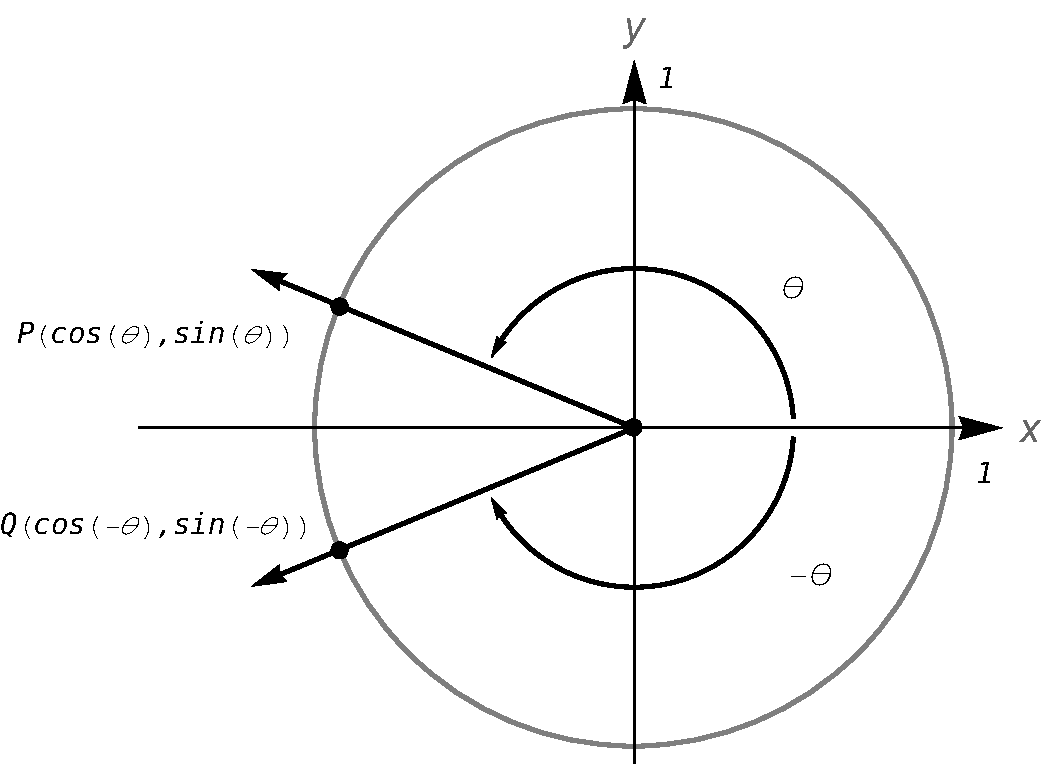
\includegraphics[width=0.5\textwidth]{fig_trans_18}
	\caption{Even/Odd identity for cosine and sine. }
	\label{fig_trans_18}
	\end{center}
\end{figure}


\ifvc\pagebreak\fi
The even/odd identities can be used to derive the sum and difference identities for cosine.

\begin{theorem}[Sum and difference identities for cosine] \label{cosinesumdifference}  
 For all angles $\alpha$ and $\beta$, it holds that
\begin{eqnarray}
\cos(\alpha + \beta) &=& \cos(\alpha) \cos(\beta) - \sin(\alpha) \sin(\beta)\,,\\[0.2cm]
\cos(\alpha - \beta) &=& \cos(\alpha) \cos(\beta) + \sin(\alpha) \sin(\beta)\,.
\end{eqnarray}
\index{cosine ! difference identity}\index{cosine ! sum identity}\index[aut]{cosinus ! somformule}\index[aut]{cosinus ! verschilformule}
\vspace{-0.5cm}
\end{theorem}
% We first prove the result for differences.  Consider the case in Figure~\ref{fig_trans_19} where $\alpha \geq \beta$.  Since the angles $\angle POQ$ and $\angle AOB$ are equal, the distance between $P$ and $Q$ is equal to the distance between $A$ and $B$; that is  

% \begin{figure}[t]
% 			\centering
% %\raisebox{0.5cm}{
% \centerline{
% \subfigure[]{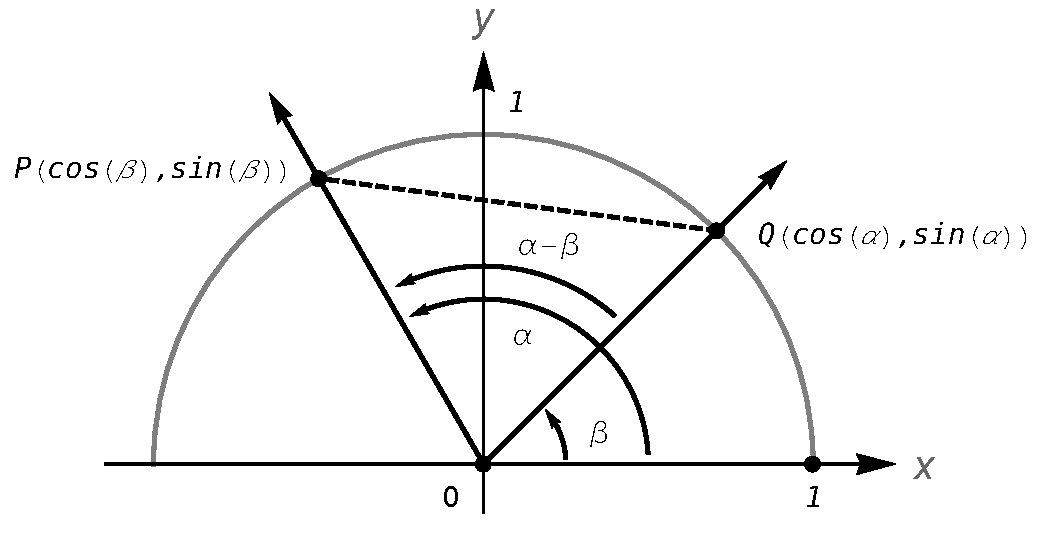
\includegraphics[width=0.5\textwidth]{fig_trans_19a}}
% \hspace{0.1cm}
% \subfigure[]{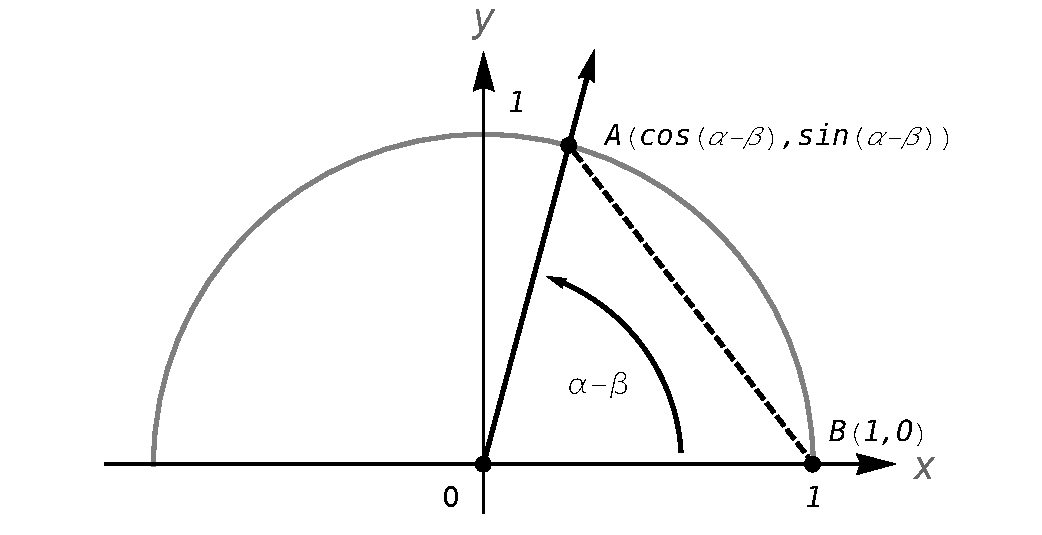
\includegraphics[width=0.5\textwidth]{fig_trans_19b}}
% }
% 	\caption{Difference identity for cosine. }
% 	\label{fig_trans_19}
% \end{figure}

% \[ \begin{array}{rcl}

% \sqrt{(\cos(\alpha) - \cos(\beta))^2 + (\sin(\alpha) - \sin(\beta))^2 } & = & \sqrt{(\cos(\alpha - \beta) - 1)^2 + (\sin(\alpha - \beta) - 0)^2}\,. \\ \end{array} \]

% Squaring both sides, we expand the left hand side of this equation as

% \[ \begin{array}{rcl}
% (\cos(\alpha) - \cos(\beta))^2 + (\sin(\alpha) - \sin(\beta))^2 
% & = &  
% \cos^2(\alpha) - 2\cos(\alpha)\cos(\beta) + \cos^2(\beta) \\  
% & & + \sin^2(\alpha) - 2\sin(\alpha)\sin(\beta)  +  \sin^2(\beta) \\ [6pt]
% & = & \cos^2(\alpha) + \sin^2(\alpha) + \cos^2(\beta) + \sin^2(\beta) \\
% & & -  2\cos(\alpha)\cos(\beta) - 2\sin(\alpha)\sin(\beta)\,. \end{array}\]

% From the Pythagorean identities, $\cos^2(\alpha) + \sin^2(\alpha) = 1$ and $\cos^2(\beta) + \sin^2(\beta) = 1$, so

% \[ \begin{array}{rcl}
% (\cos(\alpha) - \cos(\beta))^2 + (\sin(\alpha) - \sin(\beta))^2 
% & = & 2  - 2\cos(\alpha)\cos(\beta) - 2\sin(\alpha)\sin(\beta)\,. \end{array}\]

% Turning our attention to the right hand side of our equation, we find

% \[ \begin{array}{rcl}
% (\cos(\alpha - \beta) - 1)^2 + (\sin(\alpha - \beta) - 0)^2 & = & \cos^2(\alpha - \beta) - 2\cos(\alpha - \beta) + 1 + \sin^2(\alpha - \beta) \\ 
% & = & 1 +  \cos^2(\alpha - \beta) + \sin^2(\alpha - \beta) - 2\cos(\alpha - \beta)\,. \\
% \end{array} \]

% Once again, we simplify $\cos^2(\alpha - \beta) + \sin^2(\alpha - \beta)= 1$, so that

% \[ \begin{array}{rcl}
% (\cos(\alpha - \beta) - 1)^2 + (\sin(\alpha - \beta) - 0)^2 & = & 2  - 2\cos(\alpha - \beta)\,. \\ \end{array} \]

% Putting it all together, we get 
% \[ \begin{array}{rrcl}
% &2  - 2\cos(\alpha - \beta)   &=&2 - 2\cos(\alpha)\cos(\beta) - 2\sin(\alpha)\sin(\beta)\\ 
% \Leftrightarrow&\cos(\alpha - \beta) &=& \cos(\alpha)\cos(\beta) + \sin(\alpha)\sin(\beta)\,. \\\end{array} \]

% For the case where $\alpha \leq \beta$, we can apply the above argument to the angle $\beta - \alpha$ to obtain the identity  $\cos(\beta - \alpha) = \cos(\beta)\cos(\alpha) + \sin(\beta)\sin(\alpha)$.  Applying the even identity of cosine, we get $\cos(\beta - \alpha) = \cos( - (\alpha - \beta)) = \cos(\alpha - \beta)$, and we get the identity in this case, too.   


%To get the sum identity for cosine, we use the difference formula along with the even/odd identities:


%\[ \cos(\alpha + \beta) = \cos(\alpha - (-\beta)) = \cos(\alpha) \cos(-\beta) + \sin(\alpha) \sin(-\beta) = \cos(\alpha) \cos(\beta) - \sin(\alpha) \sin(\beta)\,.\]



We can  use the sum and difference identities for cosine to derive the so-called cofunction identities. The results are summarized in the following theorem.


\ifvc\pagebreak\fi
\begin{theorem}[Cofunction identities] \label{cofunctionidentities}  
For all applicable angles $\theta$, it holds that \index{Cofunction Identities}
\begin{multicols}{3}
\begin{itemize}
\item  $\cos\left(\dfrac{\pi}{2} - \theta \right) = \sin(\theta)$

\item  $\sin\left(\dfrac{\pi}{2} - \theta \right) = \cos(\theta)$

\item  $\sec\left(\dfrac{\pi}{2} - \theta \right) = \csc(\theta)$

\item  $\csc\left(\dfrac{\pi}{2} - \theta \right) = \sec(\theta)$

\item  $\tan\left(\dfrac{\pi}{2} - \theta \right) = \cot(\theta)$

\item  $\cot\left(\dfrac{\pi}{2} - \theta \right) = \tan(\theta)$
\end{itemize}
\end{multicols}

\vspace{0.1cm}
\end{theorem}
\begin{proof}
Consider for instance $\cos\left(\frac{\pi}{2} - \theta\right)$. Straightforward application of the difference identity for cosine yields:

\[ \begin{array}{rcl}

\cos\left(\dfrac{\pi}{2} - \theta\right) & = & \cos\left(\dfrac{\pi}{2}\right)\cos\left(\theta\right) + \sin\left(\dfrac{\pi}{2}\right)\sin\left(\theta \right) \\ [10pt]
                            & = & \left( 0 \right)\left( \cos(\theta) \right)  +  \left( 1 \right)\left( \sin(\theta) \right) \\ [4pt]
														& = & \sin(\theta) \,.   \\
\end{array} \]

Moreover, from this result we immediately get that 

 \[ \sin\left(\dfrac{\pi}{2} - \theta\right) = \cos\left(\dfrac{\pi}{2} -\left[\dfrac{\pi}{2} - \theta\right]\right) = \cos(\theta),\]

which says, in words, that the cosine of an angle is the sine of its complement.  Now that these identities have been established for cosine and sine, the remaining trigonometric functions follow suit.
\end{proof}

With the cofunction identities in place, we are now in the position to derive the sum and difference formulas for sine.  To achieve this, we convert to cosines using a cofunction identity, then expand using the difference formula for cosine

\[ \begin{array}{rcl}

\sin(\alpha + \beta) & = & \cos\left( \dfrac{\pi}{2} - (\alpha + \beta) \right) \\ [10pt]
                     & = & \cos\left( \left[\dfrac{\pi}{2} - \alpha \right] - \beta \right) \\ [10pt]
                     & = & \cos\left(\dfrac{\pi}{2} - \alpha \right) \cos(\beta) + \sin\left(\dfrac{\pi}{2} - \alpha \right)\sin(\beta) \\ [10pt]
                     & = & \sin(\alpha) \cos(\beta) + \cos(\alpha) \sin(\beta)\,. \\ \end{array} \]


We can derive the difference formula for sine by rewriting  $\sin(\alpha - \beta)$ as $\sin(\alpha + (-\beta))$ and using the sum formula and the even / odd identities. 


\begin{theorem}[Sum and difference identities for sine] \label{sinesumdifference} For all angles $\alpha$ and $\beta$, it holds that \index{sine ! difference identity} \index{sine ! sum identity}\index[aut]{sinus ! somformule}\index[aut]{sinus ! verschilformule}
\begin{eqnarray}
\sin(\alpha + \beta) &=& \sin(\alpha) \cos(\beta) + \cos(\alpha) \sin(\beta)\,,\\[0.2cm]
\sin(\alpha - \beta) &=& \sin(\alpha) \cos(\beta) - \cos(\alpha) \sin(\beta)\,.
\end{eqnarray}


\end{theorem}
\ifanalysis
\begin{proof}
See above.
\end{proof}
\fi

Also for the tangent function, one may derive sum and difference identities.

\begin{example}
\label{exampletangent}

 Derive a formula for $\tan(\alpha + \beta)$ in terms of $\tan(\alpha)$ and $\tan(\beta)$.

\xhrulefill{gray}{2.5pt}Solution \xhrulefill{gray}{2.5pt}

We can start expanding $\tan(\alpha + \beta)$ using a quotient identity and our sum formulas

\vspace{-.1in}

\[ \begin{array}{rcl}

\tan(\alpha + \beta) & = & \dfrac{\sin(\alpha + \beta)}{\cos(\alpha + \beta)} \\ [10pt]
                     & = & \dfrac{\sin(\alpha) \cos(\beta) + \cos(\alpha) \sin(\beta)}{\cos(\alpha) \cos(\beta) - \sin(\alpha) \sin(\beta)}\,. \\ \end{array} \]
			

Since  $\tan(\alpha) = \frac{\sin(\alpha)}{\cos(\alpha)}$ and $\tan(\beta) = \frac{\sin(\beta)}{\cos(\beta)}$, it looks as though if we divide both numerator and denominator by $\cos(\alpha) \cos(\beta)$ we will have what we want

\vspace{-.1in}
\allowdisplaybreaks
\[ \begin{array}{rcl}

\tan(\alpha + \beta) & = & \dfrac{\sin(\alpha) \cos(\beta) + \cos(\alpha) \sin(\beta)}{\cos(\alpha) \cos(\beta) - \sin(\alpha) \sin(\beta)} \cdot\dfrac{\dfrac{1}{\cos(\alpha) \cos(\beta)}}{\dfrac{1}{\cos(\alpha) \cos(\beta)}}\\
                    %&   & \\
 										%& = & \dfrac{\dfrac{\sin(\alpha) \cos(\beta)}{\cos(\alpha) \cos(\beta)} + \dfrac{\cos(\alpha) \sin(\beta)}{\cos(\alpha) \cos(\beta)}}{\dfrac{\cos(\alpha) \cos(\beta)}{\cos(\alpha) \cos(\beta)} - \dfrac{\sin(\alpha) \sin(\beta)}{\cos(\alpha) \cos(\beta)}}\\
                    &   & \\
										& = & \dfrac{\dfrac{\sin(\alpha) \cancel{\cos(\beta)}}{\cos(\alpha) \cancel{\cos(\beta)}} + \dfrac{\cancel{\cos(\alpha)} \sin(\beta)}{\cancel{\cos(\alpha)} \cos(\beta)}}{\dfrac{\cancel{\cos(\alpha)} \cancel{\cos(\beta)}}{\cancel{\cos(\alpha)} \cancel{\cos(\beta)}} - \dfrac{\sin(\alpha) \sin(\beta)}{\cos(\alpha) \cos(\beta)}}\\
                    &   & \\
										& = & \dfrac{\tan(\alpha) + \tan(\beta)}{1 -\tan(\alpha) \tan(\beta)}\,.\\
\end{array} \]

Naturally, this formula is limited to those cases where all of the tangents are defined.
\end{example}


\begin{theorem}[Sum and difference identities for tangent] \label{tangentsumdifference} For all applicable angles $\alpha$ and $\beta$, it holds that \index{tangent ! difference identity} \index{tangent ! sum identity}\index[aut]{tangens ! somformule}\index[aut]{tangens ! verschilformule}
\begin{eqnarray}
\tan(\alpha + \beta) &=& \dfrac{\tan(\alpha) + \tan(\beta)}{1 -\tan(\alpha) \tan(\beta)}\,,\\[0.2cm]
\tan(\alpha - \beta) &=&\dfrac{\tan(\alpha) - \tan(\beta)}{1 +\tan(\alpha) \tan(\beta)}\,.
\end{eqnarray}


\end{theorem}
\ifanalysis\begin{proof}
See above for sum identity. To find a formula for $\tan(\alpha - \beta)$, we can simply rewrite the difference as a sum: $\tan(\alpha + (-\beta))$.
\end{proof}
\fi




\subsubsection{Double angle identities and power reduction formulas}



\begin{theorem}[Double angle identities] \label{doubleangle}   For all applicable angles $\theta$, it holds that
\begin{eqnarray}
\cos(2\theta) &=& \cos^{2}(\theta) - \sin^{2}(\theta)\,,\\[0.2cm]
\sin(2\theta) &=& 2\sin(\theta)\cos(\theta)\,,\\[0.2cm]
\tan(2\theta) &=& \dfrac{2\tan(\theta)}{1 - \tan^{2}(\theta)}\,.
\end{eqnarray}
\index{double angle identities}\index[aut]{dubbele hoek formules}
\vspace{-0.4cm}
\end{theorem}
\begin{proof}
Specialize the sum formulas for cosine (Theorem~\ref{cosinesumdifference}), sine (Theorem~\ref{sinesumdifference}) and tangent (Theorem~\ref{tangentsumdifference}) to the case where $\alpha = \beta$.
\end{proof}
Note that the Pythagorean identity (Theorem \ref{cosinesinepythid}) allows to express $\cos(2\theta)$ alternatively as
\begin{equation}
\cos(2\theta)= 2\cos^{2}(\theta) - 1\,,
\label{doubleanglecos}
\end{equation}
and 
\begin{equation}
\cos(2\theta) = 1-2\sin^{2}(\theta)\,.
\label{doubleanglesin}
\end{equation}

In calculus, we will often be confronted with situations where it is useful to reduce the power of cosine and sine. Solving Equation~\eqref{doubleanglecos} for $\cos^{2}(\theta)$  and the Equation~\eqref{doubleanglesin} for $\sin^{2}(\theta)$ results in the aptly-named power reduction formulas below.  These are also known as \textbf{Carnot's formulas} (\textit{formules van Carnot}). 
\index{Carnot's formulas} \index[aut]{formules van Carnot}

\begin{theorem}[Power reduction formulas] \label{powerreduction} 
For all angles $\theta$, it holds that
\begin{eqnarray}
\cos^{2}(\theta) &=& \dfrac{1 + \cos(2\theta)}{2}\,,\\
\sin^{2}(\theta) &=& \dfrac{1 - \cos(2\theta)}{2}\,.
\end{eqnarray}
\index{power reduction formulas}\index[aut]{machtsreductieformules}
\vspace{-0.4cm}
\end{theorem}
\ifanalysis
\begin{proof}
See above.
\end{proof}
\fi

Not only can these formulas be used to reduce the power of cosine, they can as well be used to derive expressions for the cosine, sine and tangent of half angle. To start, we apply the power reduction formula to $\cos^{2}\left(\frac{\theta}{2}\right)$

\[ \cos^{2}\left(\dfrac{\theta}{2}\right) = \dfrac{1 + \cos\left(2 \left(\frac{\theta}{2}\right)\right)}{2} = \dfrac{1 + \cos(\theta)}{2}\,.\]

%We can obtain a formula for $\cos\left(\frac{\theta}{2}\right)$ by extracting square roots.  In a similar fashion, we obtain a half angle formula for sine, and by  using a quotient formula, obtain a half angle formula for tangent.  We summarize these formulas below.

%\ifcourse \pagebreak \fi

%\begin{theorem}[Half angle formulas] \label{halfangle}  For all applicable angles $\theta$, it holds that \index{half-angle formulas}\index[aut]{halvehoekformules}
%\begin{eqnarray}
%\cos\left(\dfrac{\theta}{2}\right) &=& \pm \sqrt{\dfrac{1 + \cos(\theta)}{2}}\,,\\[0.2cm]
%\sin\left(\dfrac{\theta}{2}\right) &=& \pm \sqrt{\dfrac{1 - \cos(\theta)}{2}}\,,\\[0.2cm]
%\tan\left(\dfrac{\theta}{2}\right) &=& \pm \sqrt{\dfrac{1 - \cos(\theta)}{1+\cos(\theta)}}\,,
%\end{eqnarray}

%\vspace{-.1in}

%where the choice of $\pm$ depends on the quadrant in which the terminal side of $\frac{\theta}{2}$ lies.

%\end{theorem}


\ifvc
\begin{example}
Verify the following identity:  
\begin{equation}
\sin(2\theta) = \dfrac{2\tan(\theta)}{1 + \tan^{2}(\theta)}\,,
\label{exdouble1}
\end{equation}
and then use it to derive the identity
\begin{equation}
\tan\left(\dfrac{\theta}{2}\right) = \dfrac{\sin(\theta)}{1+\cos(\theta)}\,.
\label{exdouble2}
\end{equation}

\xhrulefill{gray}{2.5pt}Solution \xhrulefill{gray}{2.5pt}

 We start with the right hand side of Equation~\eqref{exdouble1} and note that $1 + \tan^{2}(\theta) = \sec^{2}(\theta)$.  Then, we rewrite $\tan(\theta)$ and $\sec(\theta)$ in terms of $\cos(\theta)$ and $\sin(\theta)$:

\vspace{-.15in}

\[ \begin{array}{rcl}

\dfrac{2\tan(\theta)}{1 + \tan^{2}(\theta)} & = & \dfrac{2\tan(\theta)}{\sec^{2}(\theta)}= \dfrac{2 \left( \dfrac{\sin(\theta)}{\cos(\theta)}\right)}{\dfrac{1}{\cos^{2}(\theta)}}= 2\left( \dfrac{\sin(\theta)}{\cos(\theta)}\right) \cos^{2}(\theta) \\ [15pt]
																						& = & 2\left( \dfrac{\sin(\theta)}{\cancel{\cos(\theta)}}\right) \cancel{\cos(\theta)} \cos(\theta) = 2\sin(\theta) \cos(\theta) = \sin(2\theta)\,. \\ 

\end{array} \]


To derive Equation~\eqref{exdouble2}, we will start with the identity given by Equation~\eqref{exdouble1}  and manipulate it into the identity we are asked to prove.  It seems reasonable to proceed by replacing each occurrence of $\theta$ in Equation~\eqref{exdouble2} with $\frac{\theta}{2}$:

\vspace{-.1in}

\[ \begin{array}{rrcl} 

&\sin\left(2 \left(\dfrac{\theta}{2}\right)\right) & = &  \dfrac{2\tan\left(\dfrac{\theta}{2}\right)}{1 + \tan^{2}\left(\dfrac{\theta}{2}\right)} \\ [15pt]
\Leftrightarrow&\sin(\theta) & = & \dfrac{2\tan\left(\dfrac{\theta}{2}\right)}{1 + \tan^{2}\left(\dfrac{\theta}{2}\right)}\,. \\ \end{array} \]

We now have the $\sin(\theta)$ we need, but we somehow need to get a factor of $1+\cos(\theta)$ involved.  To get cosines involved, recall that $1 + \tan^{2}\left(\frac{\theta}{2}\right) = \sec^{2}\left(\frac{\theta}{2}\right)$.  We continue to manipulate our given identity by converting secants to cosines and using a power reduction formula

\[ \begin{array}{rrcl} 

&\sin(\theta) & = &  \dfrac{2\tan\left(\dfrac{\theta}{2}\right)}{1 + \tan^{2}\left(\dfrac{\theta}{2}\right)} \\ [15pt]
& & = & \dfrac{2\tan\left(\dfrac{\theta}{2}\right)}{\sec^{2}\left(\dfrac{\theta}{2}\right)} \\ [15pt]
& & = & 2 \tan\left(\dfrac{\theta}{2}\right) \cos^{2}\left(\dfrac{\theta}{2}\right) \\ [5pt]
& & = & 2 \tan\left(\dfrac{\theta}{2}\right) \left(\dfrac{1 + \cos\left(2 \left(\dfrac{\theta}{2}\right)\right)}{2}\right) \\ [15pt]
& & = &  \tan\left(\dfrac{\theta}{2}\right) \left(1+\cos(\theta) \right) \\ [5pt]
\Leftrightarrow&\tan\left(\dfrac{\theta}{2}\right) & = & \dfrac{\sin(\theta)}{1+\cos(\theta)}\,. \\ 
\end{array}  \]


\end{example}
\fi

\subsubsection{Product to sum formulas and vice versa}
The product to sum formulas, are easily verified by expanding each of the right hand sides in accordance with Theorems~\ref{cosinesumdifference} and \ref{sinesumdifference}.  They are of particular use in calculus, and we list them here for reference. These are also known as \textbf{Simpson's formulas} (\textit{formules van Simpson}). \index[aut]{formules van Simpson} \index{Simpson's formulas}


\begin{theorem}[Product to sum formulas] \label{producttosum}  
For all angles $\alpha$ and $\beta$, it holds that \index{product to sum formulas}\index[aut]{som-naar-product-identiteiten}\index{Simpson's formulas} \index[aut]{formules van Simpson}
\begin{eqnarray}
\cos(\alpha)\cos(\beta) &=& \frac{1}{2} \left( \cos(\alpha - \beta) + \cos(\alpha + \beta)\right)\,,\\[0.2cm]
\sin(\alpha)\sin(\beta) &=& \frac{1}{2} \left( \cos(\alpha - \beta) - \cos(\alpha + \beta)\right)\,,\\[0.2cm]
\sin(\alpha)\cos(\beta) &=& \frac{1}{2} \left( \sin(\alpha - \beta) + \sin(\alpha + \beta)\right)\,.
\end{eqnarray}

\end{theorem}
\ifanalysis
\begin{proof}
Prove as an exercise.
\end{proof}
\fi

Related to the product to sum formulas are the sum to product formulas.  These are easily verified using the product to sum formulas, and as such, their proofs are left as exercises.

\begin{theorem}[Sum to product formulas] \label{sumtoproduct}  For all angles $\alpha$ and $\beta$, it holds that 
\begin{eqnarray}
\cos(\alpha) + \cos(\beta) &=& 2 \cos\left( \dfrac{\alpha + \beta}{2}\right)\cos\left( \dfrac{\alpha - \beta}{2}\right)\,,\\[0.2cm]
\cos(\alpha) -  \cos(\beta) &=& - 2 \sin\left( \dfrac{\alpha + \beta}{2}\right)\sin\left( \dfrac{\alpha - \beta}{2}\right)\,,\\[0.2cm]
\sin(\alpha) \pm \sin(\beta) &=& 2 \sin\left( \dfrac{\alpha \pm \beta}{2}\right)\cos\left( \dfrac{\alpha \mp \beta}{2}\right)\,.
\end{eqnarray}
\index{sum to product formulas}\index[aut]{product-naar-som-identiteiten}\index{Simpson's formulas} \index[aut]{forumles van Simpson}
\end{theorem}
\ifanalysis
\begin{proof}
Prove as an exercise.
\end{proof}
\fi


\ifvc
\subsubsection{Laws of sines and cosines}
For completeness we state the laws of sines and cosines, which can be used to solve triangles -- that is, find the length of each side of a triangle and the measure of each of its angles.

For that purpose, we introduce the convention that a lower case Greek letter denotes an angle, as well as the measure of said angle,  and the corresponding lowercase English letter represents the side,  as well as the length of said side opposite that angle (Figure~\ref{fig_trans_19}).   Taken together, the pairs $(\alpha, a)$, $(\beta, b)$ and $(\gamma, c)$ are called angle side opposite pairs.  Besides, the vertex where two rays meet at an angle $\alpha$ will be denoted by the corresponding uppercase English letter, namely $A$. The Pythagorean theorem along with Equations~\eqref{cosrechthoek} and \eqref{sinrechthoek} allows us to easily handle any given right triangle problem, but what if the triangle is not a right triangle? In certain cases, we can use the \textbf{law of sines} (\textit{sinusregel}) to help. \index[aut]{sinusregel} \index{law of sines}




\begin{theorem}[The law of sines]  \label{lawofsines} \index{law of sines}\index[aut]{sinusregel}  Given a triangle with angle-side opposite pairs $(\alpha, a)$, $(\beta, b)$ and $(\gamma, c)$, the following ratios hold

\[ \frac{\sin(\alpha)}{a} = \frac{\sin(\beta)}{b} = \frac{\sin(\gamma)}{c},\]

or, equivalently,

\[ \frac{a}{\sin(\alpha)} = \frac{b}{\sin(\beta)}  = \frac{c}{\sin(\gamma)}\,. \]

\end{theorem}

This theorem enables us to solve triangles when, for instance, the given side is adjacent to both angles, the so-called Angle-Side-Angle (ASA) case, or if we are given the measure of just one of the angles in the triangle along with the length of two sides, only one of which is adjacent to the given angle (Angle-Side-Side (ASS)). Besides, it can be used to solve the Angle-Angle-Side (AAS) case. 

\begin{figure}[h]
	\begin{center}
			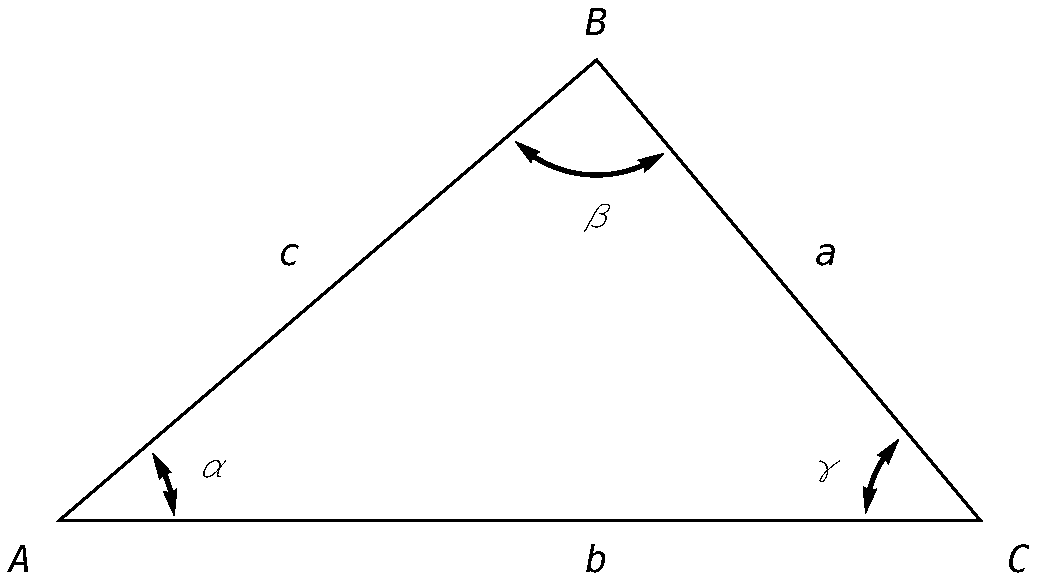
\includegraphics[width=0.5\textwidth]{fig_trans_19}
	\caption{Naming convention for angles, sides and vertices of triangles. }
	\label{fig_trans_19}
	\end{center}
\end{figure}

Now, we recall the \textbf{law of cosines} (\textit{cosinusregel}) which handles solving triangles in the  Side-Angle-Side (SAS) and Side-Side-Side (SSS) cases.
\index{law of cosinus} \index[aut]{cosinusregel}

\begin{theorem}[Law of cosines] \label{lawofcosines} \index{law of cosines} \index[aut]{cosinusregel}  
Given a triangle with angle-side opposite pairs $(\alpha, a)$, $(\beta, b)$ and $(\gamma, c)$, the following equations hold
\[ a^2 = b^2 + c^2 - 2bc \cos(\alpha)\,, \qquad  b^2 = a^2 + c^2 - 2ac \cos(\beta)\,,  \qquad   c^2 = a^2 + b^2 - 2ab \cos(\gamma)\,,  \]

or, solving for the cosine in each equation, we have
 
\[ \cos(\alpha) = \dfrac{b^2+c^2 - a^2}{2bc}\,, \qquad \cos(\beta) = \dfrac{a^2+c^2 - b^2}{2ac}\,, \qquad \cos(\gamma) = \dfrac{a^2+b^2 - c^2}{2ab}\,. \]

\end{theorem}


We illustrate the use of Theorems~\ref{lawofsines} and \ref{lawofcosines} in the following example.

\begin{example}
\label{losex} Solve the following triangles. 
\begin{multicols}{2}

\begin{enumerate}

\item   $\alpha = 120^{\circ}$, $a = 7$, $\beta = 45^{\circ}$
\item  $\alpha = 30^{\circ}$, $a=4$, $c = 4$
\item   $\beta = 50^{\circ}$, $a = 7$, $c=2$ 

\end{enumerate}

\end{multicols}

\xhrulefill{gray}{2.5pt}Solution \xhrulefill{gray}{2.5pt}

\begin{enumerate}

\item Knowing an angle-side opposite pair, namely $\alpha$ and $a$, we may proceed in using the law of sines.  Since $\beta = 45^{\circ}$, we use $\frac{b}{\sin\left(45^{\circ}\right)} = \frac{7}{\sin\left(120^{\circ}\right)}$ so $b = \frac{7\sin\left(45^{\circ}\right)}{\sin\left(120^{\circ}\right)} = 7\frac{\sqrt{2}}{\cancel{2}}\frac{\cancel{2}}{\sqrt{3}}= \frac{7\sqrt{6}}{3} \approx 5.72$.  Now that we have two angle-side pairs, it is time to find the third.  To find $\gamma$, we use the fact that the sum of the measures of the angles in a triangle is $180^{\circ}$. Hence, $\gamma = 180^{\circ} - 120^{\circ} - 45^{\circ} = 15^{\circ}$.  To find $c$, we use $\gamma = 15^{\circ}$ and use the given angle-side opposite pair $(\alpha, a)$. The law of sines gives us  $\frac{c}{\sin\left(15^{\circ}\right)} = \frac{7}{\sin\left(120^{\circ}\right)}$ so that $c = \frac{7\sin\left(15^{\circ}\right)}{\sin\left(120^{\circ}\right)} \approx 2.09$.


\item  We use  the  law of sines  to find that $\frac{\sin(\gamma)}{4} = \frac{\sin\left(30^{\circ}\right)}{4}$ so that $\sin(\gamma) = \frac{1}{2}$.  Since $\gamma$ must inhabit a triangle with $\alpha = 30^{\circ}$, we must have $0^{\circ} < \gamma < 150^{\circ}$.   Since the  measure of $\gamma$ must be strictly less than $150^{\circ}$, there is just one angle what satisfies both required conditions, namely $\gamma = 30^{\circ}$.  So $\beta = 180^{\circ} - 30^{\circ} - 30^{\circ} = 120^{\circ}$ and, using the law of sines one last time, $b = \frac{4\sin\left(120^{\circ}\right)}{\sin\left(30^{\circ}\right)} =\frac{4\sin\left(60^{\circ}\right)}{\sin\left(30^{\circ}\right)} = 4\sqrt{3} \approx 6.93$.

\item  We are given the lengths of two sides, $a=7$ and $c = 2$, and the measure of the included angle, $\beta = 50^{\circ}$.  With no angle-side opposite pair to use, we apply  the law of cosines.  We get  $b^2 = 7^2 + 2^2 - 2(7)(2)\cos\left(50^{\circ}\right)$ which yields $b = \sqrt{53-28\cos\left(50^{\circ}\right)} \approx 5.92$ units.  In order to determine the measures of the remaining angles $\alpha$ and $\gamma$, we are forced to used the derived value for $b$. There are two ways to proceed at this point.  We could use the law of cosines again, or, since  we have the angle-side opposite pair $(\beta, b)$ we could use the law of sines. The advantage to using the former over the latter in cases like this is that unlike the sine function, the cosine function distinguishes between acute and obtuse angles. Indeed, the cosine of an acute is positive, whereas the cosine of an obtuse angle is negative.  We proceed with the law of cosines.  When using this method, it is always best to find the measure of the largest unknown angle first, since this will give us the obtuse angle of the triangle if there is one.  Since the largest angle is opposite the longest side, we choose to find $\alpha$ first. To that end, we use the formula $\cos(\alpha) = \frac{b^2+c^2-a^2}{2bc}$ and substitute $a = 7$, $b =  \sqrt{53-28\cos\left(50^{\circ}\right)}$ and $c = 2$. We get after simplifying \[\cos(\alpha) = \frac{2-7\cos\left(50^{\circ}\right)}{\sqrt{53-28\cos\left(50^{\circ}\right)}}\,.\]  Since $\alpha$ is an angle in a triangle, we know the radian measure of $\alpha$ must lie between $0^{\circ}$ and $180^{\circ}$.  This matches the range of the arccosine function (see Section~\ref{sec_inverse_trig}), so we have \[\alpha = \arccos\left(\frac{2-7\cos\left(50^{\circ}\right)}{\sqrt{53-28\cos\left(50^{\circ} \right)}}\right) \, \approx  114.99^{\circ}\,.\] At this point, we could find $\gamma$ using $\gamma = 180^{\circ} - \alpha - \beta \approx 180^{\circ} - 114.99^{\circ} - 50^{\circ} = 15.01^{\circ}$, that is if we trust our approximation for $\alpha$.


\end{enumerate}

\end{example}


The laws of sines and cosines are especially useful in applications, as illustrated in the following example. 

\begin{example} \label{losapplication}

Schiermonnikoog lies off the Dutch coast.  Two sightings, taken 5 kilometres apart, are made to the island.  The angle between the shore and the island at the first observation point is $30^{\circ}$ and at the second point the angle is $45^{\circ}$.  Assuming a straight coastline, find the distance from the second observation point to the island.  What point on the shore is closest to the island? How far is the island from this point?  

\xhrulefill{gray}{2.5pt}Solution \xhrulefill{gray}{2.5pt}


 We sketch the problem  with the first observation point labelled as $P$ and the second as $Q$ (Figure~\ref{fig_trans_20}). In order to use the law of sines to find the distance $d$ from $Q$ to the island, we first need to find the measure of $\beta$ which is the angle opposite the side of length $5$ kilometres.  To that end, we note that the angles $\gamma$ and $45^{\circ}$ are supplemental, so that $\gamma = 180^{\circ} - 45^{\circ} = 135^{\circ}$.  We can now find $\beta_1 = 180^{\circ} - 30^{\circ} - \gamma =  180^{\circ} - 30^{\circ} - 135^{\circ} = 15^{\circ}$. By the law of sines, we have $\frac{d}{\sin\left(30^{\circ}\right)} = \frac{5}{\sin\left(15^{\circ}\right)}$ which gives $d = \frac{5\sin\left(30^{\circ}\right)}{\sin\left(15^{\circ}\right)} \approx 9.66$ kilometres.  Next, to find the point on the coast closest to the island, which we have labelled as $C$, we need to find the perpendicular distance from the island to the coast. Let $x$ denote the distance from the second observation point $Q$ to the point $C$  and let $y$ denote the distance from $C$ to the island.  Using Equation~\eqref{cosrechthoek}, we get $\sin\left(45^{\circ}\right) = \frac{y}{d}$.  After some rearranging, we find $y = d \sin\left(45^{\circ}\right) \approx 9.66 \left(\frac{\sqrt{2}}{2}\right) \approx 6.83$ kilometres.  Hence, the island is approximately $6.83$ kilometres from the coast. To find the distance from $Q$ to $C$, we note that $\beta_2 = 180^{\circ} - 90^{\circ} - 45^{\circ} = 45^{\circ}$ so by symmetry, we get $x = y \approx 6.83$ kilometres.  Hence, the point on the shore closest to the island is approximately $6.83$ kilometres down the coast from the second observation point.

\begin{figure}[H]
	\begin{center}
			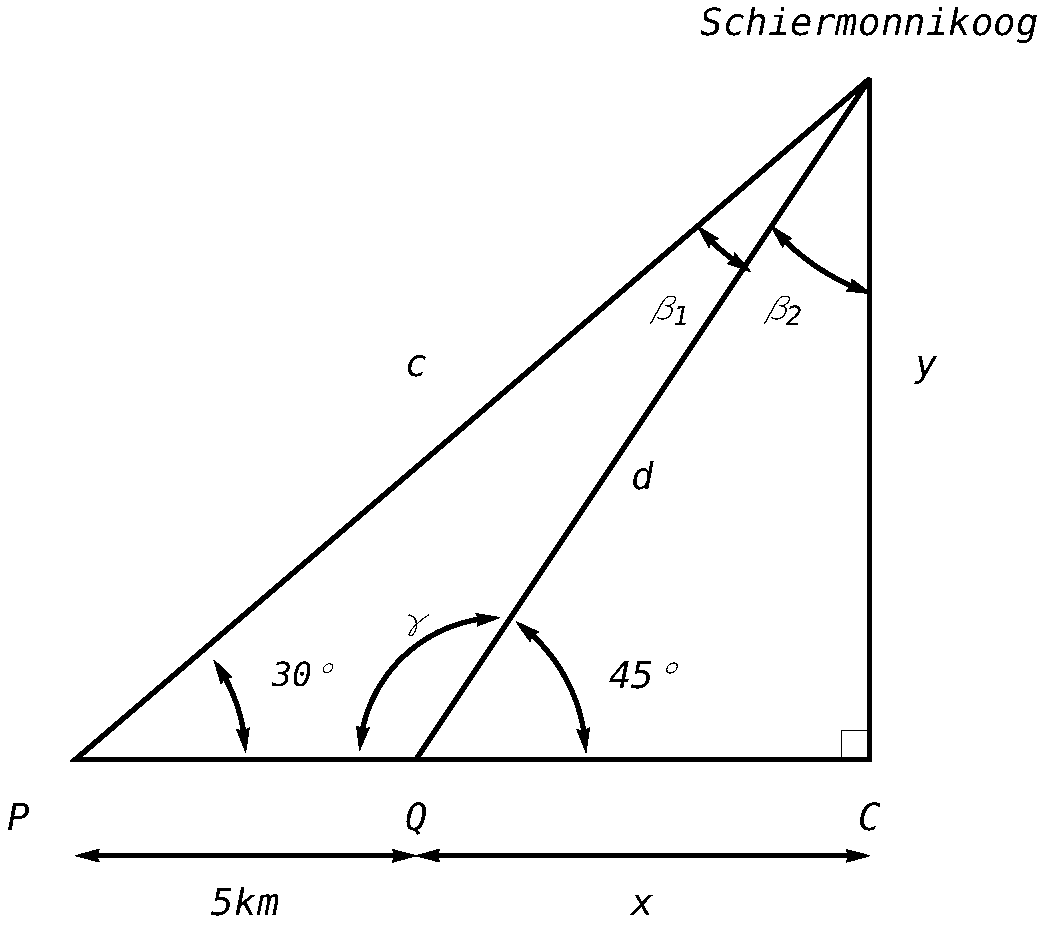
\includegraphics[width=0.4\textwidth]{fig_trans_20}
	\caption{Finding the closest distance from the Dutch coast to Schiermonnikoog. }
	\label{fig_trans_20}
	\end{center}
\end{figure}

This problem can as well be solved like we proceeded in Example~\ref{exmaple} using right triangles. 

\end{example}	
\fi





\subsection{Graphs of cosine and sine functions}
\subsubsection{Domain and range}
In the same way we studied polynomial, rational, exponential, and logarithmic functions, we will study the trigonometric functions $f(x) = \cos(x)$ and $g(x) = \sin(x)$.  The first order of business is to find the domains and ranges of these functions.  Whether we think of identifying the real number $x$ with the angle $\theta = x$ radians, or think of wrapping an oriented arc around the unit circle to find coordinates on the unit circle, it should be clear that both the cosine and sine functions are defined for all real numbers $x$.  So $\dom\,\cos(x)=\dom\, \sin(x)=\mathbb{R}$, and likewise $\im\, \cos(x)=\im\,\sin(x)=[-1,1]$.   

\subsubsection{Graphs}
The even/odd identities in Theorem~\ref{evenodd} tell us $\cos(-x) = \cos(x)$ for all real numbers $x$ and $\sin(-x) = -\sin(x)$ for all real numbers $x$.  This means $f(x) = \cos(x)$ is an even function, while $g(x) = \sin(x)$ is an odd function (see Chapter~\ref{chap_functions}). Another important property of these  functions is that  $\cos(x + 2\pi k) = \cos(x)$ and $\sin(x + 2\pi k) = \sin(x)$, for all real numbers $x$ and any integer $k$; that is the sine and cosine functions are periodic with period $2\pi$. One last property of the functions $f(x) = \cos(x)$ and $g(x) = \sin(x)$ is worth pointing out:   the graphs of both of these functions have no jumps, gaps, holes in the graph,  asymptotes, corners or cusps.  

To graph $y = \cos(x)$, we make a table using some of the common values of $x$ in the interval $[0,2\pi]$ (Table~\ref{tab_trans_2bis}). This generates a portion of the cosine graph, which we call the \index{fundamental cycle}\index[aut]{fundamentele cyclus}\textbf{fundamental cycle} (\textit{fundamentele cyclus}) of $y = \cos(x)$ (Figure~\ref{fig_trans_21a}). \index{cosine ! graph }\index[aut]{cosinus ! grafiek}




\begin{table}[H]
\caption{Cosine and sine of some common angles.}
\label{tab_trans_2bis}
\renewcommand{\arraystretch}{2.5}
\[ \begin{array}{r||rrrrrrrrr}  
 x & 0 & \dfrac{\pi}{4}& \dfrac{\pi}{2}  & \dfrac{3\pi}{4}  &\pi &\dfrac{5\pi}{4}  &\dfrac{3\pi}{2}  &\dfrac{7\pi}{4}  &2\pi\\ \hline
\cos(x) & 1 
  & \dfrac{\sqrt{2}}{2} & 0 &-\dfrac{\sqrt{2}}{2} &-1 &-\dfrac{\sqrt{2}}{2}&0& \dfrac{\sqrt{2}}{2}  & 1\\[0.2cm]
  \sin(x)&0&\dfrac{\sqrt{2}}{2}&1&\dfrac{\sqrt{2}}{2}&0&-\dfrac{\sqrt{2}}{2}&-1&-\dfrac{\sqrt{2}}{2}&0\\
\end{array} \] 
\renewcommand{\arraystretch}{1}
\end{table}

To get the graph of the cosine function for intervals stretching beyond the fundamental cycle, we way imagine copying and pasting this graph end to end infinitely in both directions (left and right) on the $x$-axis (Figure~\ref{fig_trans_21c}).

\begin{figure}
\centering
%\raisebox{0.5cm}{
\centerline{
\subfigure[\label{fig_trans_21a}]{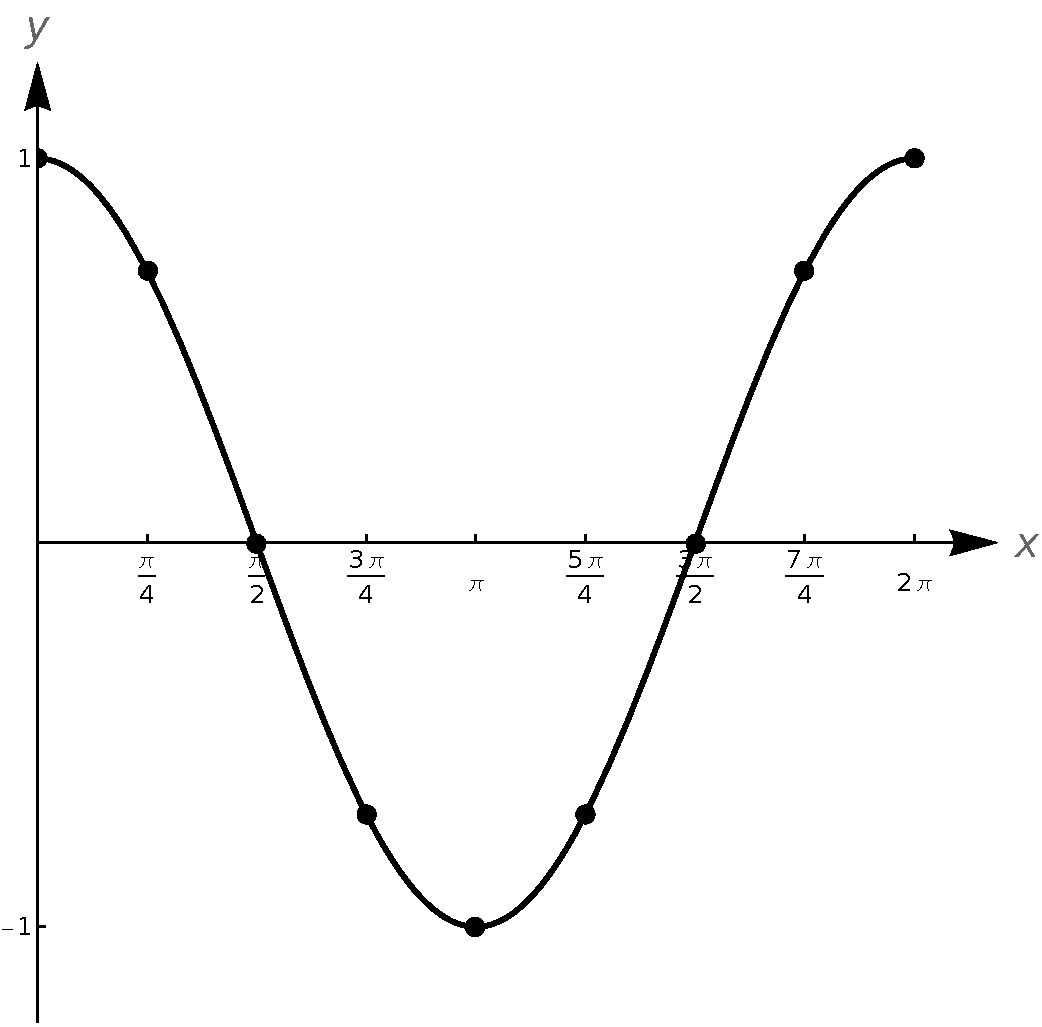
\includegraphics[width=0.4\textwidth]{fig_trans_21a}}
\hspace{1cm}
\subfigure[\label{fig_trans_21b}]{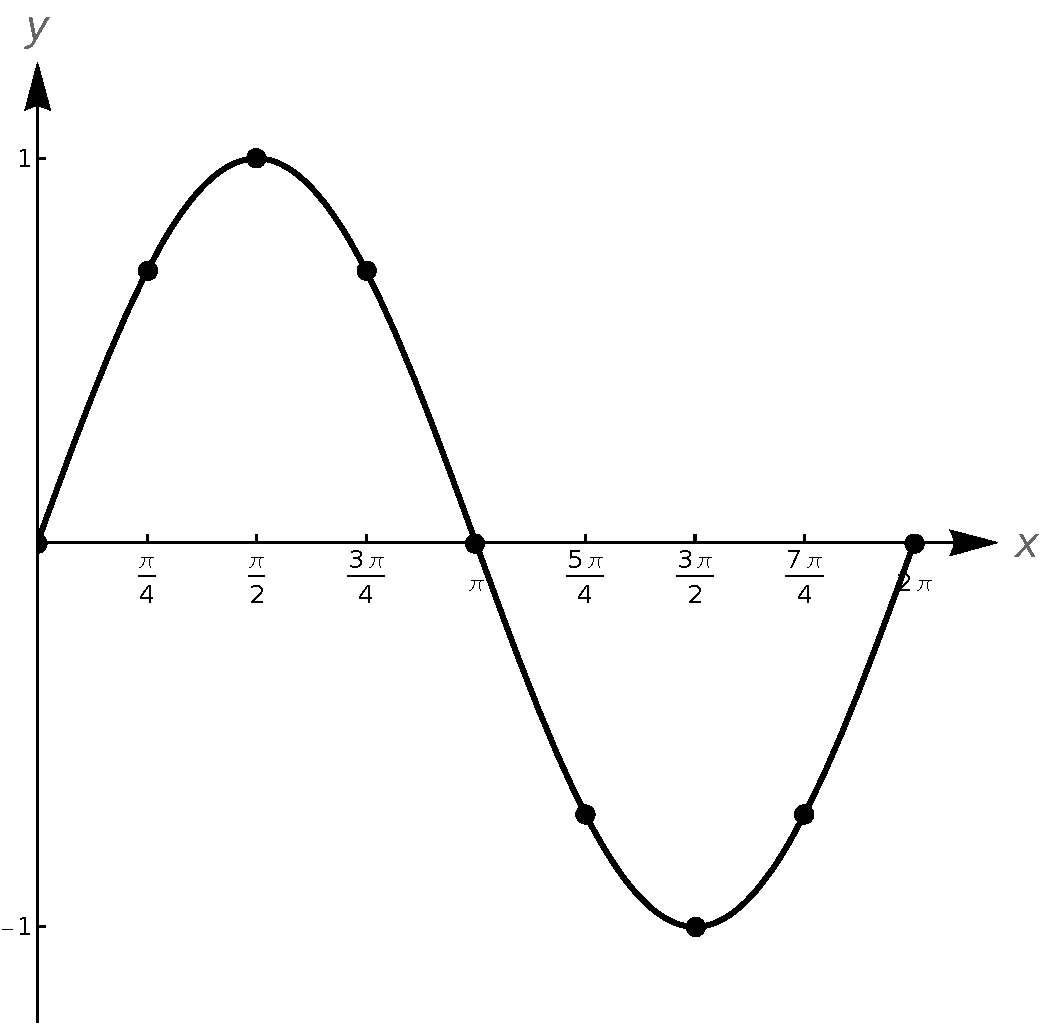
\includegraphics[width=0.4\textwidth]{fig_trans_21b}}
}
\centering\subfigure[\label{fig_trans_21c}]{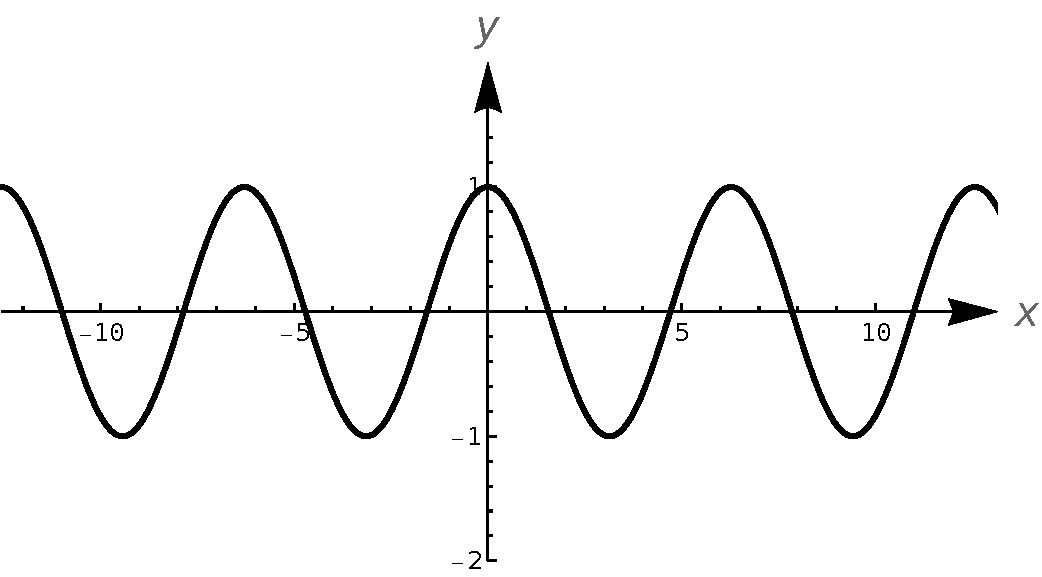
\includegraphics[width=0.6\textwidth]{fig_trans_21c}}\\
\centering\subfigure[\label{fig_trans_21d}]{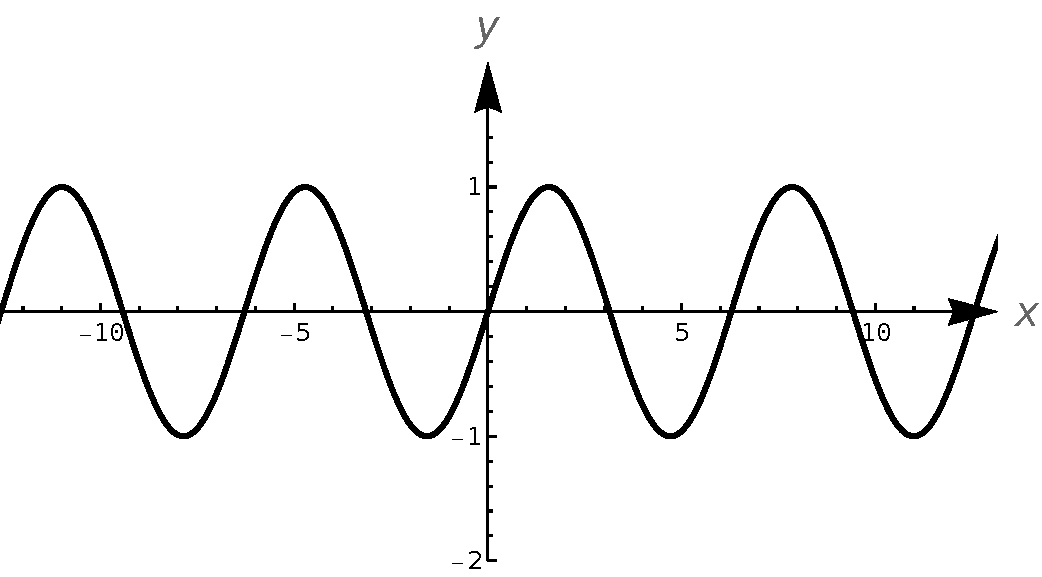
\includegraphics[width=0.6\textwidth]{fig_trans_21d}}
	\caption{Graphs of the fundamental cycle (a,b) and four such cycles (c,d) of $y=\cos(x)$ (a,c) and $y=\sin(x)$ (b,d).}
\end{figure}

We can plot the fundamental cycle of the graph of $y = \sin(x)$ similarly, with similar results (Figures~\ref{fig_trans_21b} and~\ref{fig_trans_21d})\index{sine ! graph}\index[aut]{sinus ! grafiek}. It is of course no accident that the graphs of $y = \cos(x)$ and $y = \sin(x)$ are so similar.  Using a cofunction identity (Theorem~\ref{cofunctionidentities}) along with the even property of cosine, we have
\[ \sin(x) = \cos\left(\frac{\pi}{2} - x\right) = \cos\left(-\left(x - \frac{\pi}{2}\right)\right) = \cos\left(x - \frac{\pi}{2}\right)\]





Recalling Section~\ref{sec_transformations}, we see from this formula that the graph of $y=\sin(x)$ is the result of shifting the graph of $y = \cos(x)$ to the right $\frac{\pi}{2}$ units.




Now that we know the basic shapes of the graphs of $y = \cos(x)$ and $y = \sin(x)$, we can rely on the tools from Section~\ref{sec_transformations} to graph more complicated curves.  To do so, we need to keep track of the movement of some key points on the original graphs, such as  $x = 0$, $\frac{\pi}{2}$, $\pi$, $\frac{3\pi}{2}$ and $2\pi$.

\ifcalculus
\begin{example}  \label{cosinesinegraphex1} 
Graph one cycle of the following functions. State the period of each.

\begin{multicols}{2}

\begin{enumerate}

\item  $f(x) = 3 \cos\left(\dfrac{\pi x - \pi}{2}\right) + 1$

\item  $g(x) = \dfrac{1}{2} \sin(\pi - 2x) + \dfrac{3}{2}$

\end{enumerate}

\end{multicols}

\xhrulefill{gray}{2.5pt}Solution \xhrulefill{gray}{2.5pt}

\begin{enumerate}

\item  We set the argument of the cosine, $\frac{\pi x - \pi}{2}$, equal to each of the values:  $0$, $\frac{\pi}{2}$, $\pi$, $\frac{3\pi}{2}$, $2\pi$ and solve for $x$. This leads to $x$-values 1, 2, 3, 4 and 5. Next, we substitute each of these $x$-values into $f(x)$ to determine the corresponding $y$-values and connect the dots in a pleasing wavelike fashion (Figure~\ref{fig_trans_22a}). One cycle is graphed on $[1,5]$ so the period is the length of that interval which is $4$.
\renewcommand{\arraystretch}{1.5}
\[ \begin{array}{r||rrrrr}  
x                                      &1 &2 &3  &4 &5\\ \hline
& & & & & \\[-0.6cm]
\cos\left(\dfrac{\pi x - \pi}{2}\right)&1 &0 &-1 &0 &1\\
f(x)                                   &4 &1 &-2 &1 &4
\end{array} \]
\renewcommand{\arraystretch}{1}
%Gekanteld:
%\renewcommand{\arraystretch}{1.5}
%\[ \begin{array}{r|cc}  
% x &\cos\left(\dfrac{\pi x - \pi}{2}\right) & f(x) \\ \hline\hline
%1 &\hphantom{-}1& \hphantom{-}4 \\ 
%2 &\hphantom{-}0& \hphantom{-}1 \\ 
%3 &-1& -2 \\ 
%4 &\hphantom{-}0& \hphantom{-}1 \\ 
%5 &-1& \hphantom{-}4  \\ 
%\end{array} \]
%\renewcommand{\arraystretch}{1}


\item  Again, we set the argument of the sine, $\pi - 2x$, equal to each of our quarter marks, being  $0$, $\frac{\pi}{2}$, $\pi$, $\frac{3\pi}{2}$, $2\pi$ and  solve for $x$, which leads to $x$-values $\frac{\pi}{2}$, $\frac{\pi}{4}$, 0, $-\frac{\pi}{4}$ and $-\frac{\pi}{2}$. We now find the corresponding $y$-values on the graph by substituting each of these $x$-values into  $g(x) = \frac{1}{2} \sin(\pi - 2x) + \frac{3}{2}$.  


%\renewcommand{\arraystretch}{1.5}
%\[ \begin{array}{r||rrrrr}  
%x                                      &1 &2 &3  &4 &5\\ \hline
%& & & & & \\[-0.6cm]
%\cos\left(\dfrac{\pi x - \pi}{2}\right)&1 &0 &-1 &0 &1\\
%f(x)                                   &4 &1 &-2 &1 &4
%\end{array} \]
%\renewcommand{\arraystretch}{1}

\renewcommand{\arraystretch}{2}
\[ \begin{array}{r||rrrrr}  
x &\hphantom{-}\dfrac{\pi}{2} & \hphantom{-}\dfrac{\pi}{4} & \hphantom{-}0 & \hphantom{-}-\dfrac{\pi}{4} & \hphantom{-}-\dfrac{\pi}{2} \\[0.1cm] \hline
\sin\left(\pi - 2x\right) & 0 & 1 & 0 & -1 & 0 \\ 
f(x) & \dfrac{3}{2} & 2 & \dfrac{3}{2} & 1 & \dfrac{3}{2} \\ 
\end{array} \]


Once again, we connect the dots in a wavelike fashion (Figure~\ref{fig_trans_22b}). One cycle was graphed on the interval $\left[ -\frac{\pi}{2}, \frac{\pi}{2}\right]$ so the period is $\frac{\pi}{2} - \left(-\frac{\pi}{2}\right) = \pi$. 
\end{enumerate}
\begin{figure}[H]
			\centering
%\raisebox{0.5cm}{
\centerline{
\subfigure[\label{fig_trans_22a}]{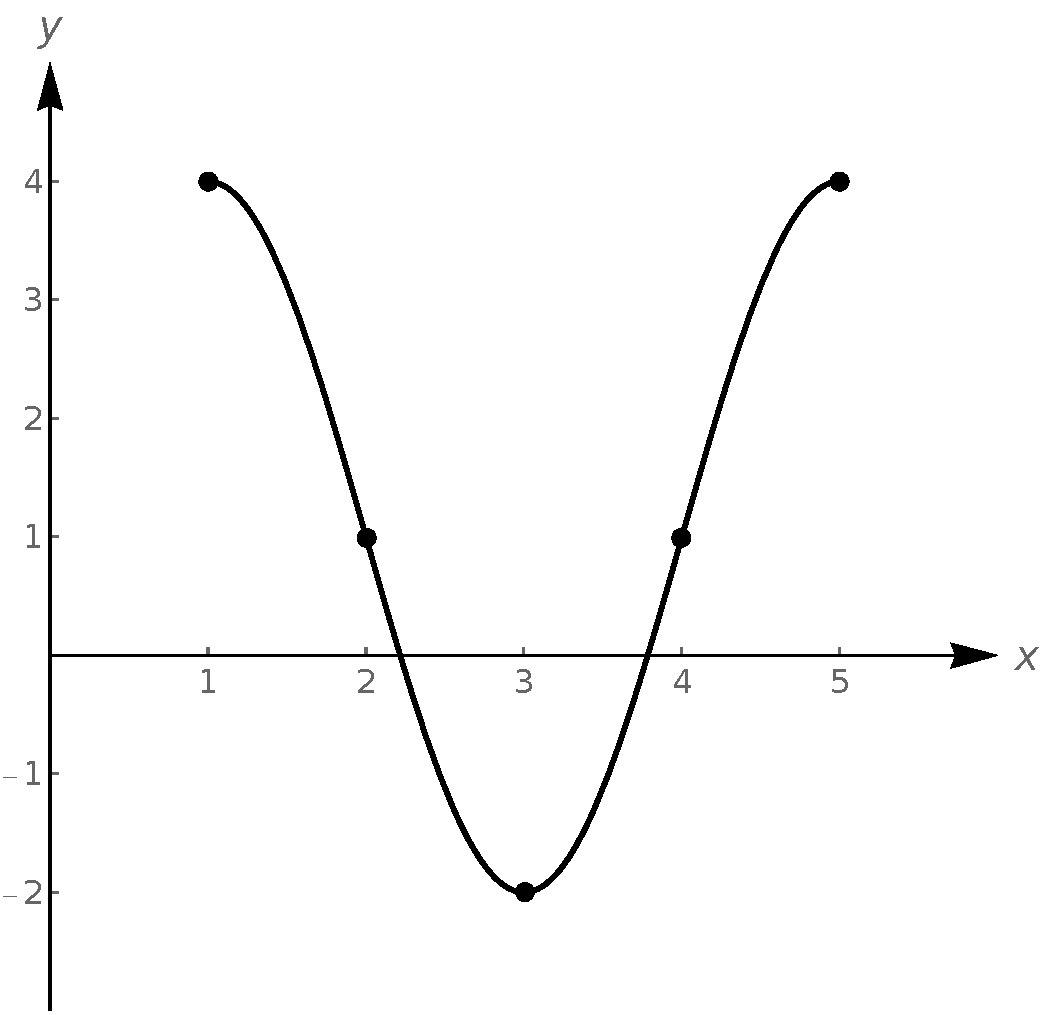
\includegraphics[width=0.45\textwidth]{fig_trans_22a}}
\hspace{0.1cm}
\subfigure[\label{fig_trans_22b}]{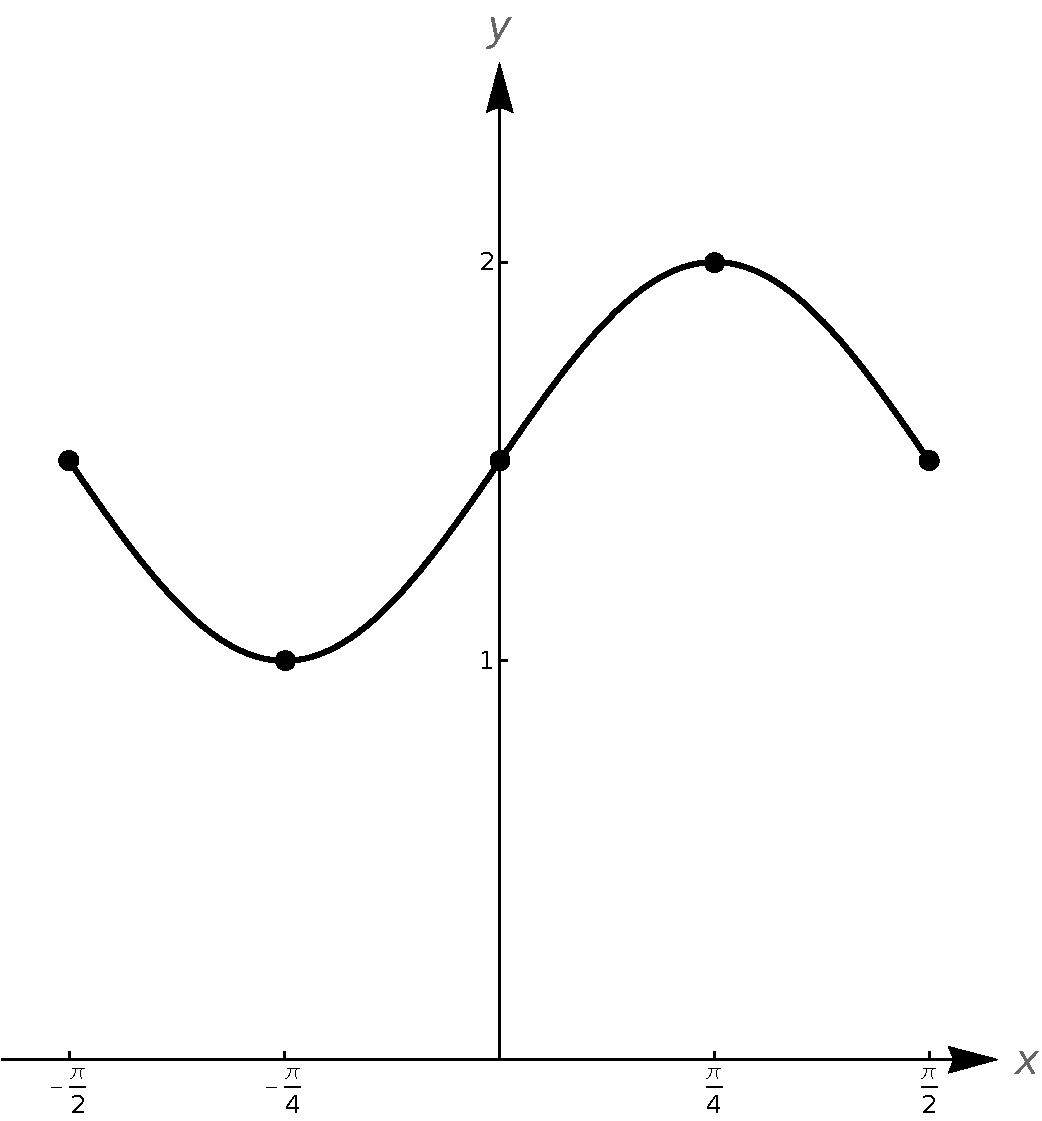
\includegraphics[width=0.45\textwidth]{fig_trans_22b}}
}
	\caption{The of $f(x) = 3 \cos\left(\frac{\pi x - \pi}{2}\right) + 1$ (a) and $g(x) = \frac{1}{2} \sin(\pi - 2x) + \frac{3}{2}$ (b).}
\end{figure}

\end{example}
\fi

\ifcourse
\ifcalculus
The functions in Example~\ref{cosinesinegraphex1} are examples of \textbf{sinusoids} (\textit{sinuso\"ide}) \index{sinusoid}\index[aut]{sinuso\"ide}. Roughly speaking, a sinusoid is the result of taking the basic graph of $f(x) = \cos(x)$ or $g(x) = \sin(x)$ and performing any of the transformations mentioned in Section~\ref{sec_transformations}.
\fi 
\ifanalysis
By performing any of the transformations mentioned in Section~\ref{sec_transformations} to the the basic graph of $f(x) = \cos(x)$ or $g(x) = \sin(x)$, we arrive at so-called \textbf{sinusoids} (\textit{sinuso\"ide}) \index{sinusoid}\index[aut]{sinuso\"ide}.
\fi
Sinusoids can be characterized by four properties:  period, amplitude, phase shift and vertical shift. More specifically, for the functions

\[y = A \cos(\omega x + \phi) + B \quad \text{and} \quad y= A \sin(\omega x + \phi) + B ,\]
or equivalently,
\[y = A \cos\left[\omega \left(x + \frac{\phi}{\omega}\right)\right] + B \quad \text{and} \quad y= A \sin\left[\omega \left(x + \frac{\phi}{\omega}\right)\right] + B ,\]
we have:
\begin{itemize}

\item   period $\dfrac{2\pi}{\omega}$

\item   amplitude $|A|$

\item   phase shift $-\dfrac{\phi}{\omega}$

\item   vertical shift $B$

\end{itemize}
for $\omega>0$. Here, $\phi$ is called the \textbf{phase} (\textit{fase}) of the sinusoid, while $\omega$ is nothing but the angular velocity.  It is the number of cycles the sinusoid completes over a $2\pi$ interval. \index{phase}\index[aut]{fase}\index{angular velocity}\index[aut]{hoeksnelheid}

\fi


\subsection{Graphs of the other trigonometric functions}

Before constructing the graphs of the other trigonometric functions, we first determine their domains and ranges. 

\subsubsection{Domain and range}
Starting from the domain and range of the cosine and sine functions, we can now determine the domains and ranges of the other trigonometric functions. 

For what concerns the function $f(x) = \sec(x) = \frac{1}{\cos(x)}$.  We know that it is undefined whenever \\ $\cos(x) = 0$.  Since we know $\cos(x) = 0$ whenever $x = \frac{\pi}{2} + \pi k$ for integers $k$, the domain of this function, in set builder notation is  
$$\dom\,\sec(x)=\left\{ x : x \neq  \frac{\pi}{2} + \pi k, \forall k \in\mathbb{Z} \right\}\,.$$

Using interval notation to describe this set, we get  
\[\dom\,
\sec(x) = \ldots \cup \left] -\frac{5\pi}{2}, -\frac{3\pi}{2}\right[ \cup \left] -\frac{3\pi}{2}, -\frac{\pi}{2}\right[ \cup  \left]-\frac{\pi}{2}, \frac{\pi}{2}\right[ \cup \left]\frac{\pi}{2}, \frac{3\pi}{2}\right[ \cup  \left]\frac{3\pi}{2}, \frac{5\pi}{2}\right[ \cup \ldots \]

This is, however,  a very cumbersome notation.   In order to write this in a more compact way, we note that from the set-builder description of the domain, the $k$th point excluded from the domain, which we will call $x_k$, and which is given by  $x_k = \frac{(2k+1)\pi}{2}$. Hence, the domain of $f(x) = \sec(x)$ consists of the intervals determined by successive points 
$x_k$:   
$$\left]x_k, x_{k+1}\right[ = \left] \frac{(2k+1)\pi}{2},  \frac{(2k+3)\pi}{2}\right[\,,$$
where $k = 0$, $\pm 1$, $\pm 2$, \ldots.  The union of infinitely many such intervals can be written as

\[\dom\,
\sec(x) =  \bigcup_{k = -\infty}^{+\infty} \left] \frac{(2k+1)\pi}{2}, \frac{(2k+3) \pi}{2} \right[\,. \]

To determine the range of  $f(x) = \sec(x)$, we appeal to the definition $\sec(x) = \frac{1}{\cos(x)}$ and recall that the range of $f(x) = \cos(x)$ is $[-1,1]$. Since $f(x) = \sec(x)$ is  undefined when $\cos(x) = 0$, we split our discussion into two cases: when $0 < \cos(x) \leq 1$ and when $-1 \leq \cos(x) < 0$.  If the former case we can divide the inequality $\cos(x) \leq 1$ by  $\cos(x)$ to obtain  $\sec(x) = \frac{1}{\cos(x)} \geq 1$. Moreover,  we have that as  $\cos(x) \rightarrow  0^+$, $\sec(x) \rightarrow +\infty$. If, on the other hand, if $-1 \leq \cos(x) < 0$, then dividing by $\cos(x)$ causes a reversal of the inequality so that $\sec(x) = \frac{1}{\cos(x)} \leq -1$.  In this case, as $\cos(x) \rightarrow  0^-$, we get $\sec(x) \rightarrow -\infty$. Since $f(x) = \cos(x)$ admits all of the values in $[-1,1]$, the function $f(x) = \sec(x)$ admits all of the values in $\left.\right]-\infty, -1] \cup [1,+\infty\left[\right.$.  Using set-builder notation, the range of $f(x) = \sec(x)$ can be written as $$\im\,\sec(x)=\{ u : u \leq -1 \vee u \geq 1 \}=\{ u :|u| \geq 1 \}.$$ 

 Similar arguments can be used to determine the domains and ranges of the remaining three circular functions: $\csc(x)$, $\tan(x)$ and $\cot(x)$.  The reader is encouraged to do so. The results are summarized in Table~\ref{tab_trans_3}.

\renewcommand{\arraystretch}{3}%
\begin{table}[h!]
\caption{Domains and ranges of the trigonometric functions.}
\label{tab_trans_3}
\begin{tabular}{c|c|c}
Function & Domain & Range \\ \hline\hline
$f(x)=\sin(x)$& $\mathbb{R}$ &$[-1,1]$ \\ [5pt] \hline
$f(x)=\cos(x)$ & $\mathbb{R}$ & $[-1,1]$ \\ [5pt] \hline
$f(x)=\sec(x)$ &$ \displaystyle{\bigcup_{k = -\infty}^{\infty} \left] \frac{(2k+1)\pi}{2}, \frac{(2k+3) \pi}{2} \right[}$  & $\{ u : |u| \geq 1 \} = \, ]-\infty, -1] \cup [1, +\infty[ $ \\[10pt] \hline
$f(x)=\csc(x)$ & $\displaystyle{\bigcup_{k = -\infty}^{\infty} \left]k \pi ,(k+1) \pi \right[}$ & $\{ u : |u| \geq 1 \} = \, ]-\infty, -1] \cup [1, +\infty[ $  \\ [10pt] \hline
$f(x)=\tan(x)$&$ \displaystyle{\bigcup_{k = -\infty}^{\infty} \left] \frac{(2k+1)\pi}{2}, \frac{(2k+3) \pi}{2} \right[}$  & $\mathbb{R}$ \\ [10pt]  \hline
$f(x)=\cot(x)$&$\displaystyle{\bigcup_{k = -\infty}^{\infty} \left]k \pi ,(k+1) \pi \right[}$ &$\mathbb{R}$\\ [10pt]
\end{tabular}
\end{table}
\renewcommand{\arraystretch}{1}%

\ifanalysis
\subsubsection{Graphs of secant and cosecant functions}
  Since $\sec(x) = \frac{1}{\cos(x)}$, we can use our table of values for the graph of $y = \cos(x)$ and take reciprocals. We already know from Table~\ref{tab_trans_3} that the domain of $f(x) = \sec(x)$ excludes all odd multiples of $\frac{\pi}{2}$. As $x \underset{<}{\rightarrow} \frac{\pi}{2}$, $\cos(x) \rightarrow  0^+$, so $\sec(x) \rightarrow +\infty$. Similarly, we find that  as $x \underset{>}{\rightarrow}  \frac{\pi}{2}$, $\sec(x) \rightarrow -\infty$;  as $x \underset{<}{\rightarrow}\frac{3\pi}{2}$, $\sec(x) \rightarrow -\infty$; and as $x \underset{>}{\rightarrow}  \frac{3\pi}{2}$, $\sec(x) \rightarrow +\infty$.  This means we have a pair of vertical asymptotes to the graph of $y = \sec(x)$, $x = \frac{\pi}{2}$ and $x = \frac{3\pi}{2}$.  Since $\cos(x)$ is periodic with period $2\pi$, it follows that $\sec(x)$ is also.  In Figure~\ref{fig_trans_23a} we graph a fundamental cycle of $y = \sec(x)$, while Figure~\ref{fig_trans_23c} shows four cycles.  \index{secant ! graph}\index[aut]{secans ! grafiek}.

As one would expect, to graph $y = \csc(x)$ we begin with $y = \sin(x)$ and take reciprocals of the corresponding $y$-values.  Here, we encounter issues at $x = 0$, $x = \pi$ and $x = 2\pi$.  We graph the fundamental cycle of $y = \csc(x)$ in Figure~\ref{fig_trans_23b} along with the dotted graph of $y=\sin(x)$ for reference.  Since $y = \sin(x)$ and $y = \cos(x)$ are merely phase shifts of each other, so too are $y = \csc(x)$ and $y = \sec(x)$. This can be seen easily in Figure~\ref{fig_trans_23d} showing four cycles. \index{cosecant ! graph}\index[aut]{cosecans ! grafiek}

\begin{figure}
			\centering
%\raisebox{0.5cm}{
\centerline{
\subfigure[\label{fig_trans_23a}]{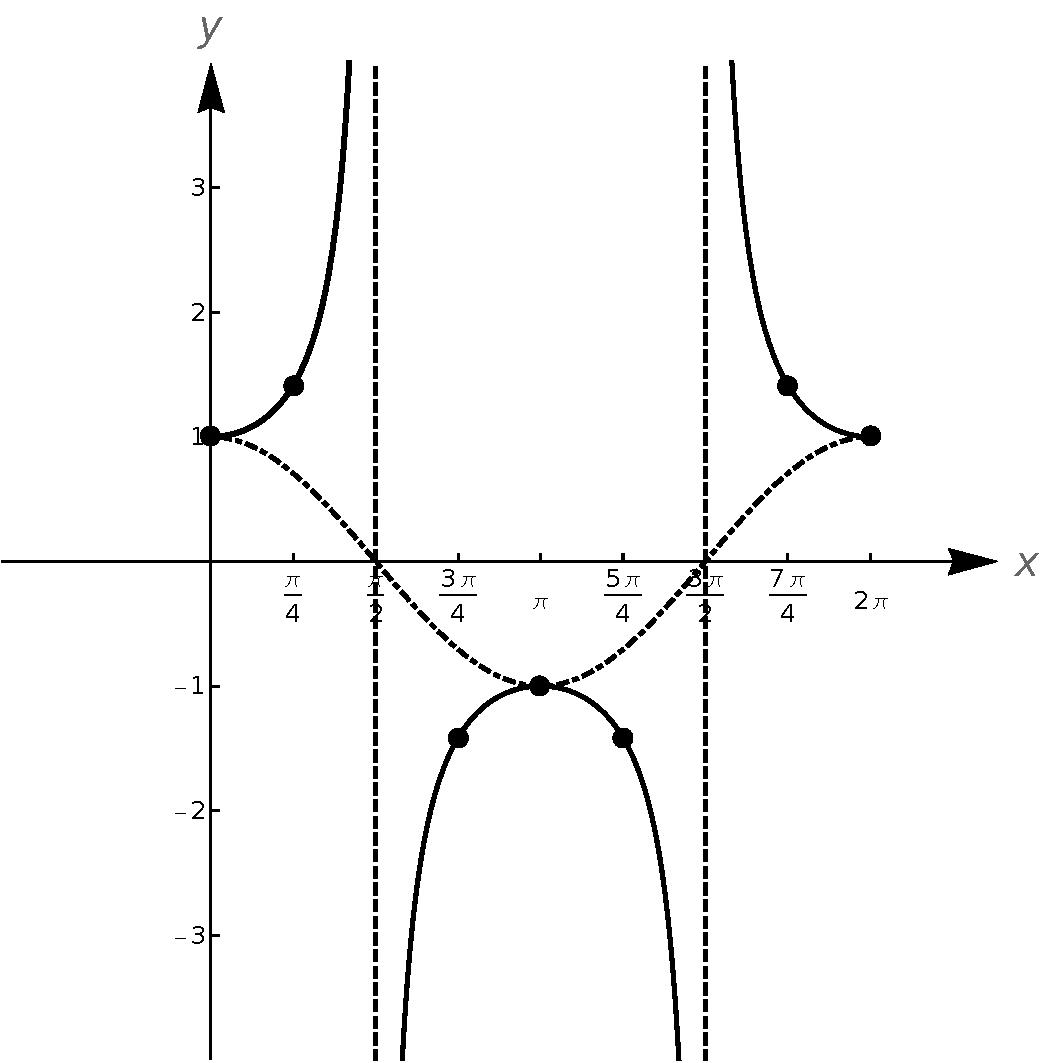
\includegraphics[width=0.45\textwidth]{fig_trans_23a}}
\hspace{0.1cm}
\subfigure[\label{fig_trans_23b}]{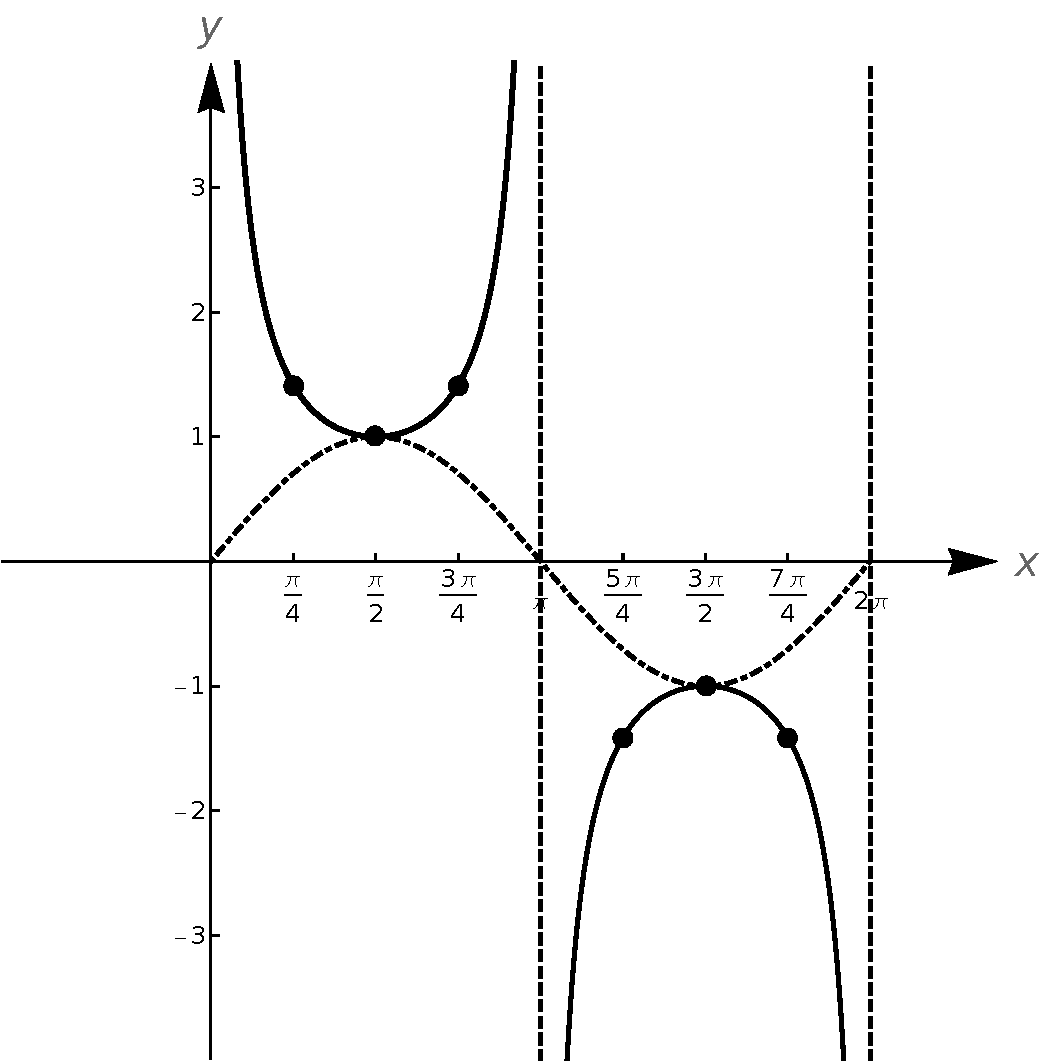
\includegraphics[width=0.45\textwidth]{fig_trans_23b}}
}
\centering\subfigure[\label{fig_trans_23c}]{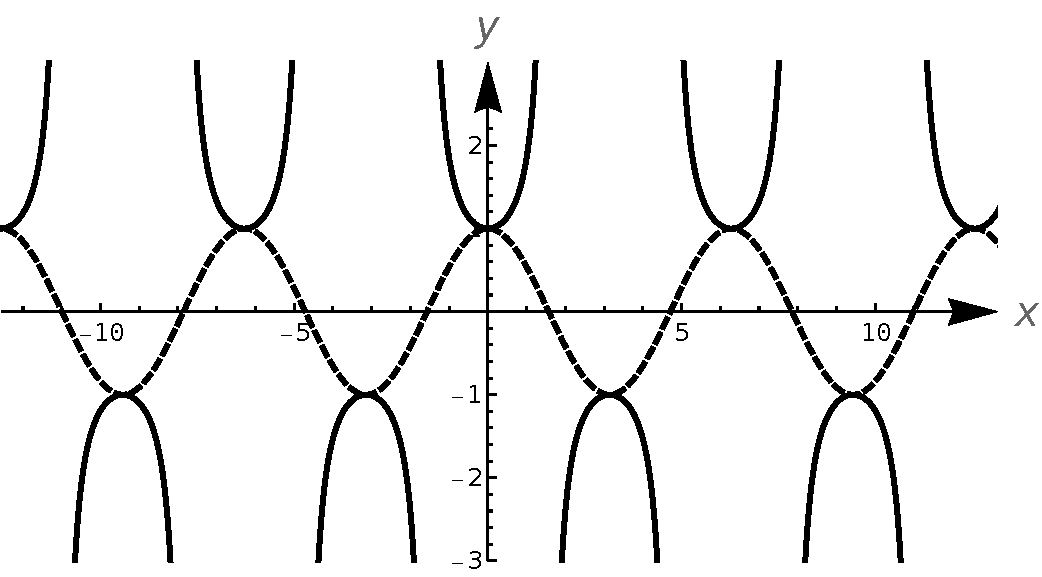
\includegraphics[width=0.65\textwidth]{fig_trans_23c}}\\
\centering\subfigure[\label{fig_trans_23d}]{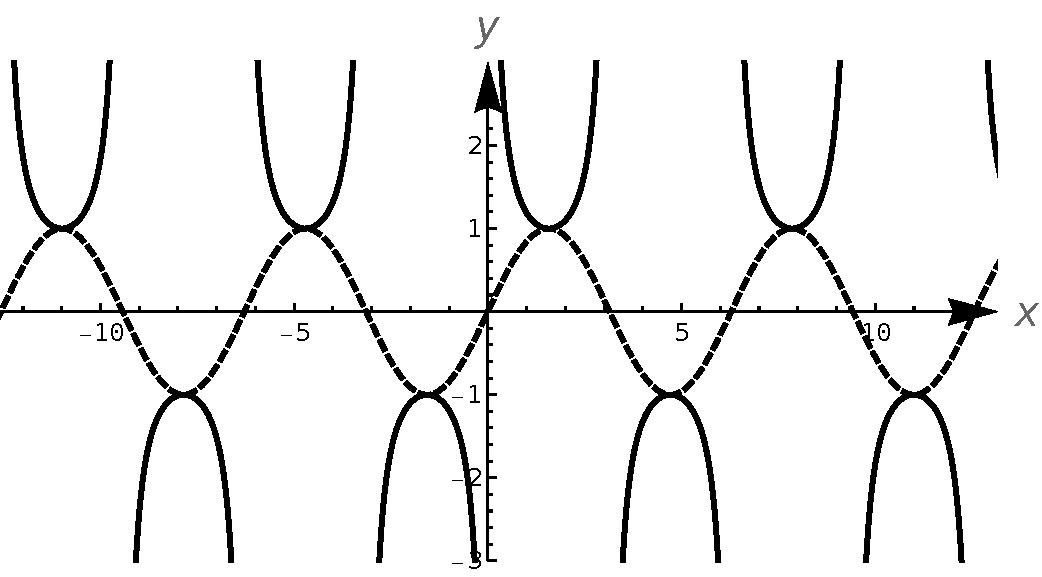
\includegraphics[width=0.65\textwidth]{fig_trans_23d}}\\
	\caption{The fundamental cycle (a,b) and four cycles (c,d) of $y=\sec(x)$ (a,c) and $y=\csc(x)$ (b,d), superimposed on the graph of $y=\cos(x)$ and $y=\sin(x)$, respectively.}
\end{figure}
\fi

\subsubsection{Graphs of tangent and cotangent functions}
Finally, we turn our attention to the graphs of the tangent and cotangent functions.  When constructing a table of values for the tangent function, we see that $y = \tan(x)$ is undefined at $x  = \frac{\pi}{2}$ and $x = \frac{3\pi}{2}$.  As $x \underset{<}{\rightarrow} \frac{\pi}{2}$, $\sin(x) \rightarrow 1^{-}$ and $\cos(x) \rightarrow 0^{+}$, so that $\tan(x)  = \frac{\sin(x)}{\cos(x)}\rightarrow +\infty$ producing a vertical asymptote at $x = \frac{\pi}{2}$.  Using a similar analysis, we get that as $x \underset{>}{\rightarrow} \frac{\pi}{2}$, $\tan(x) \rightarrow -\infty$; as $x \underset{<}{\rightarrow} \frac{3\pi}{2}$, $\tan(x) \rightarrow +\infty$; and as $x \underset{>}{\rightarrow} \frac{3\pi}{2}$, $\tan(x) \rightarrow -\infty$.  Plotting this information yields the graph in Figures~\ref{fig_trans_24a} and \ref{fig_trans_24c}. \index{tangent ! graph}\index[aut]{tangens ! grafiek}


\begin{figure}
			\centering
%\raisebox{0.5cm}{
\centerline{
\subfigure[\label{fig_trans_24a}]{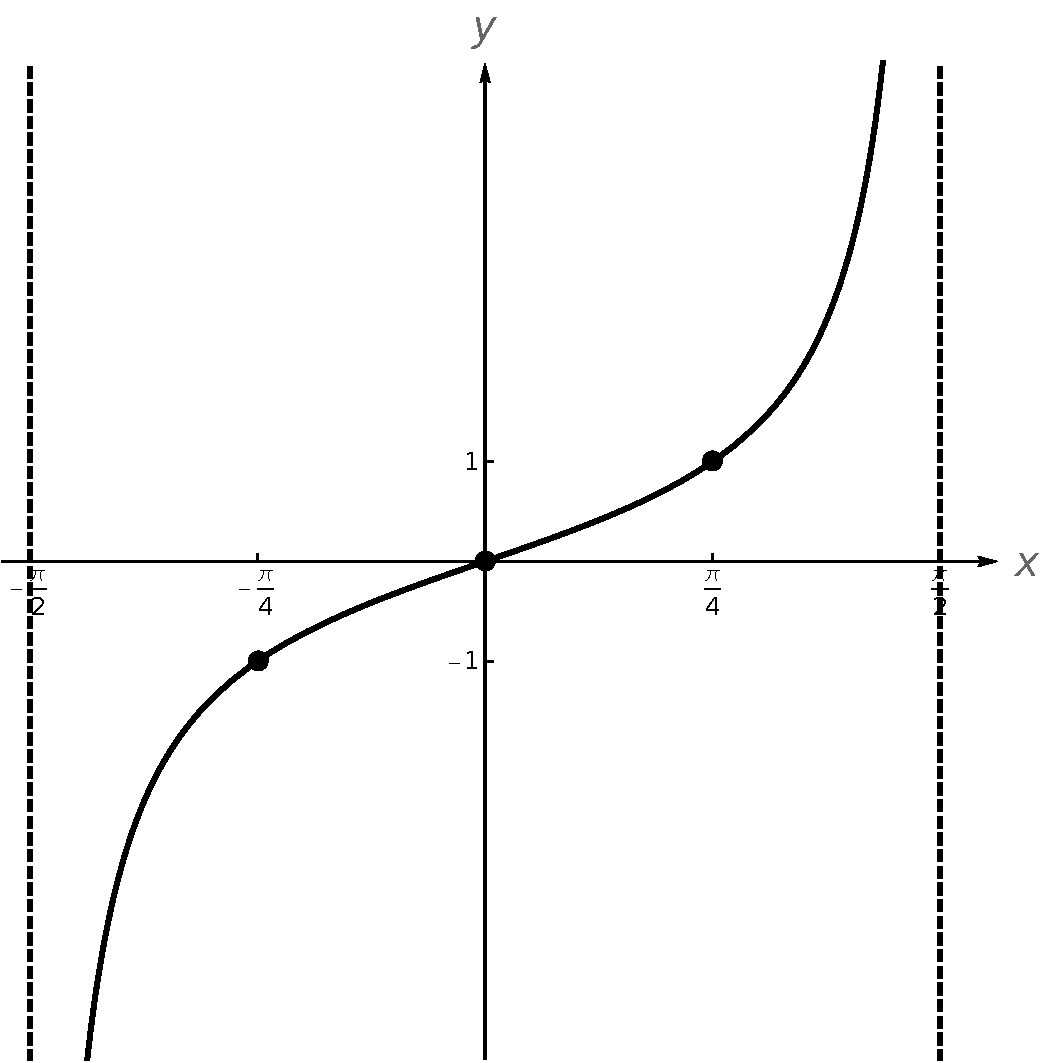
\includegraphics[width=0.45\textwidth]{fig_trans_24a}}
\hspace{0.1cm}
\subfigure[\label{fig_trans_24b}]{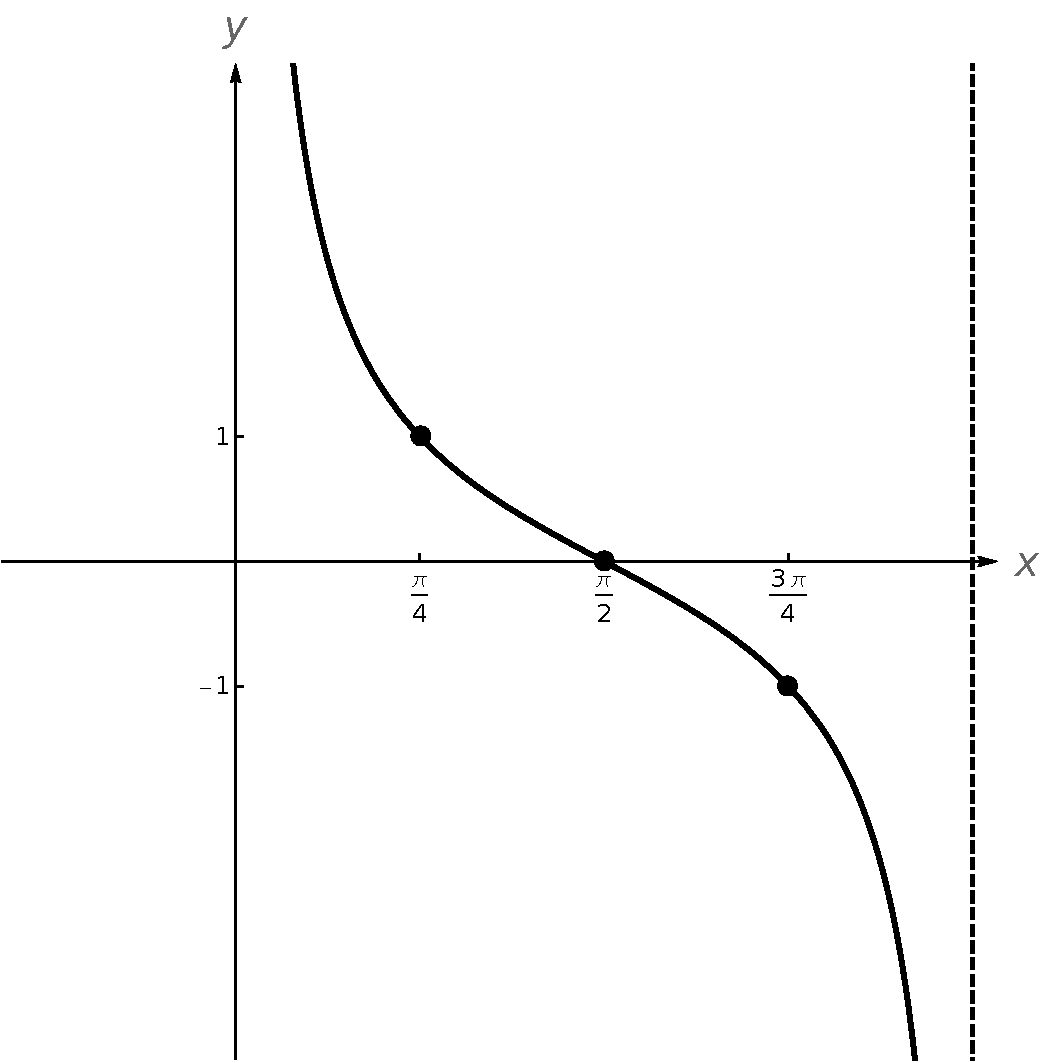
\includegraphics[width=0.45\textwidth]{fig_trans_24b}}
}
\centering\subfigure[\label{fig_trans_24c}]{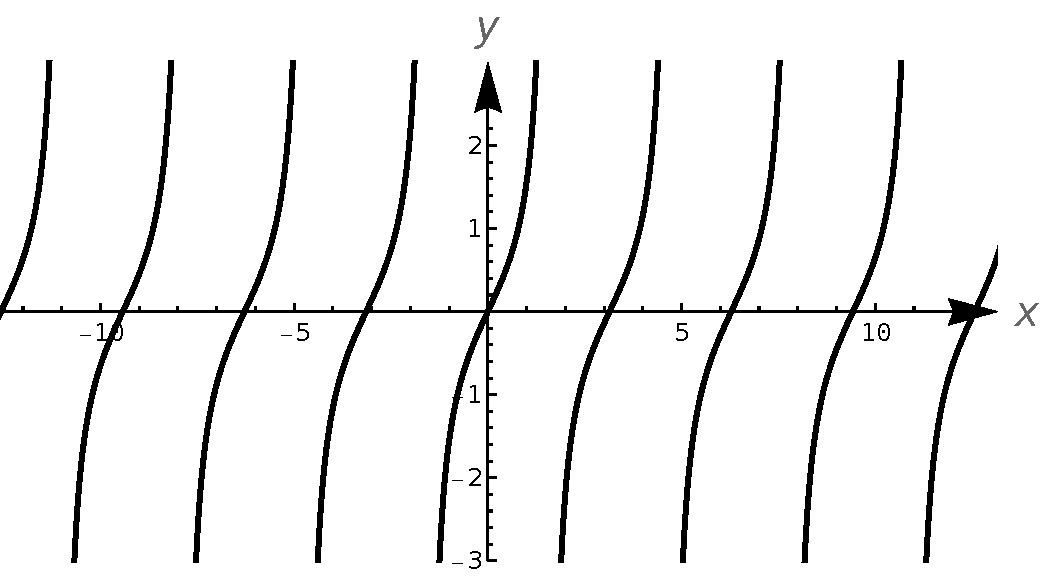
\includegraphics[width=0.65\textwidth]{fig_trans_24c}}\\
\centering\subfigure[\label{fig_trans_24d}]{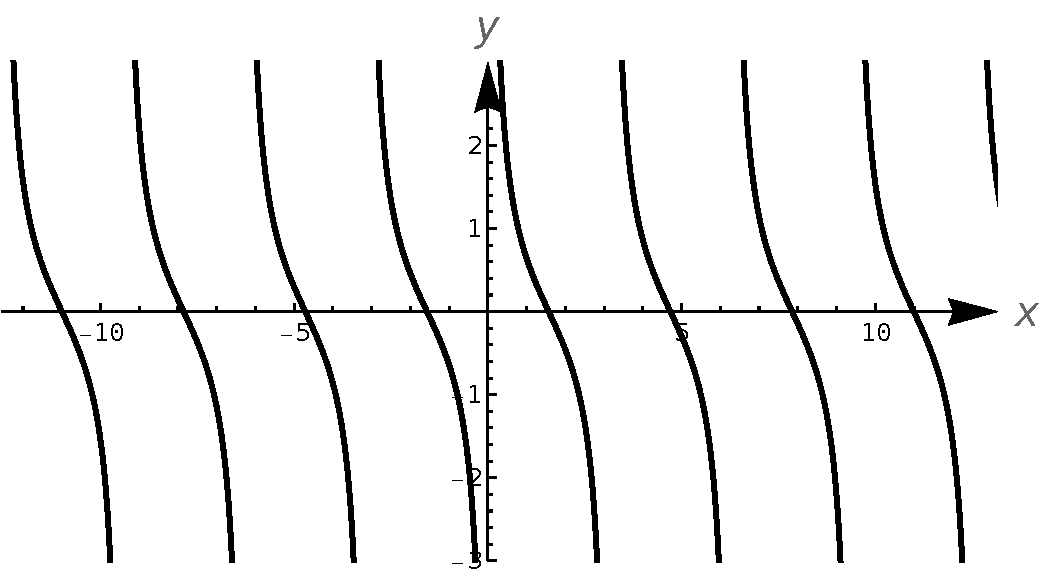
\includegraphics[width=0.65\textwidth]{fig_trans_24d}}\\
	\caption{The fundamental cycle (a,b) and eight cycles (c,d) of $y=\tan(x)$ (a,c) and $y=\cot(x)$ (b,d).}
\end{figure}


From this graph, it appears as if the tangent function is periodic with period $\pi$.  To prove that this is the case, we appeal to the sum formula for tangents.  We have: 

\[ \tan(x+\pi) = \dfrac{\tan(x) + \tan(\pi)}{1 - \tan(x) \tan(\pi)} = \dfrac{\tan(x) + 0}{1 - (\tan(x) )(0)} = \tan(x),\]

which tells us the period of $\tan(x)$ is at most $\pi$.  To show that it is exactly $\pi$, suppose $p$ is a positive real number so that $\tan(x+p) = \tan(x)$ for all real numbers $x$.  For $x=0$, we have $\tan(p) = \tan(0+p) = \tan(0) = 0$, which means $p$ is a multiple of $\pi$.  The smallest positive multiple of $\pi$ is $\pi$ itself, so we have established the result. We take as our fundamental cycle for $y=\tan(x)$ the interval $\left[-\frac{\pi}{2}, \frac{\pi}{2}\right]$.

It should be no surprise that $y = \cot(x)$ behaves similarly to $y = \tan(x)$.  \index{cotangent ! graph}\index[aut]{cotangens ! grafiek} It clearly appears from Figures~\ref{fig_trans_24b} and~\ref{fig_trans_24d} as if the period of $\cot(x)$ is $\pi$, and we leave it to the reader to prove this.  We take as one fundamental cycle the interval $[0,\pi]$.





\begin{example}
 \label{seccscgraphex} Graph one cycle of the following functions.  State the period of each.

\begin{multicols}{2}

\begin{enumerate}

\item  $f(x) = 1 - 2 \sec(2x)$

\item  $g(x) = 2\cot\left(\dfrac{\pi}{2} x + \pi\right) + 1$

\end{enumerate}

\end{multicols}

\xhrulefill{gray}{2.5pt}Solution \xhrulefill{gray}{2.5pt}

\begin{enumerate}

\item  To graph $f(x) = 1 - 2 \sec(2x)$, we first set the argument of secant, $2x$, equal to $0$, $\frac{\pi}{2}$, $\pi$, $\frac{3\pi}{2}$ and $2\pi$ and solve for $x$, to get 0, $\frac{\pi}{4}$, $\frac{\pi}{2}$, $\frac{3\pi}{4}$, $\pi$. Next, we substitute these $x$-values into $f(x)$.  If $f(x)$ exists, we have a point on the graph in Figure~\ref{fig_trans_25a};  otherwise, we have found a vertical asymptote.  In addition to these points and asymptotes, we have graphed the associated cosine curve (dashed curve), being $y = 1 - 2 \cos(2x)$.  Since one cycle is graphed over the interval $[0,\pi]$, the period is $\pi - 0 = \pi$.

\renewcommand{\arraystretch}{2}
\[ \begin{array}{r||ccccc}  
x         & \hphantom{-}0  & \hphantom{-}\dfrac{\pi}{4} & \hphantom{-}\dfrac{\pi}{2}  &  \hphantom{-}\dfrac{3\pi}{4} & \hphantom{-}\pi   \\[0.1cm] \hline 
\sec(2x)  &  \hphantom{-}1  & \hphantom{-}\text{undefined}  & -1  &  \hphantom{-}\text{undefined} & 1 \\
 f(x)   & \hphantom{-}-1  & \hphantom{-}\text{undefined}  & 3  &  \hphantom{-}\text{undefined} & -1 \\
\end{array} \]
\renewcommand{\arraystretch}{1}
%
%Gekanteld:
%\renewcommand{\arraystretch}{2}
%\[ \begin{array}{r|cc}  
%x               &\sec(2x)      & f(x) \\ \hline\hline
%0               &\hphantom{-}1      & -1 \\
%\dfrac{\pi}{4}  &\hphantom{-}\text{undefined}   &\hphantom{-}\text{undefined} \\
%\dfrac{\pi}{2} &-1  &\hphantom{-}3\\
%-\dfrac{3\pi}{4} &\text{undefined}             &\hphantom{-}\text{undefined} \\
%\pi &\hphantom{-}1  & -1\\
%\end{array} \]
%\renewcommand{\arraystretch}{1}

\item We take $0$, $\frac{\pi}{4}$, $\frac{\pi}{2}$, $\frac{3\pi}{4}$ and $\pi$ as quarter marks for constructing the fundamental cycle of the cotangent curve.  To graph this function, we begin by setting $\frac{\pi}{2} x + \pi$ equal to each such mark and solve for $x$, to arrive at $-2$, $\frac{-3}{2}$, $-1$, $\frac{-1}{2}$ and $0$. We now use these $x$-values to generate our graph (Figure~\ref{fig_trans_25b}). We find the period to be $0 - (-2) = 2$. 

\renewcommand{\arraystretch}{2}
\[ \begin{array}{r||ccccc}  
x         & \hphantom{-}-2  & \hphantom{-}-\dfrac{3}{2}  & \hphantom{-}-1  &  \hphantom{-}-\dfrac{1}{2} & 0  \\[0.1cm] \hline 
\cot\left(\dfrac{\pi}{2}x+\pi\right)  &  \hphantom{-}\text{undefined}  & \hphantom{-}1 & 0  &  \hphantom{-}-1 & \hphantom{-}\text{undefined} \\
g(x)  &  \hphantom{-}\text{undefined}  & \hphantom{-}3 & 1  &  \hphantom{-}-1 & \hphantom{-}\text{undefined} \\
\end{array} \]
\renewcommand{\arraystretch}{1}

%Gekanteld:
%\renewcommand{\arraystretch}{2}
%\[ \begin{array}{r|cc}  
%x               &\cot\left(\dfrac{\pi}{2}x+\pi\right)      & g(x) \\ \hline\hline
%-2          &\hphantom{-}\text{undefined}   &\hphantom{-}\text{undefined} \\
%-\dfrac{3}{2}     &\hphantom{-}1   &\hphantom{-}3 \\
%-1          &\hphantom{-}0   &\hphantom{-}1 \\
%-\dfrac{1}{2}     &-1              &-1 \\
%0          &\hphantom{-}\text{undefined}   &\hphantom{-}\text{undefined} \\ 
%\end{array} \]
%\renewcommand{\arraystretch}{1}


\end{enumerate}

\begin{figure}[H]
			\centering
%\raisebox{0.5cm}{
\centerline{
\subfigure[\label{fig_trans_25a}]{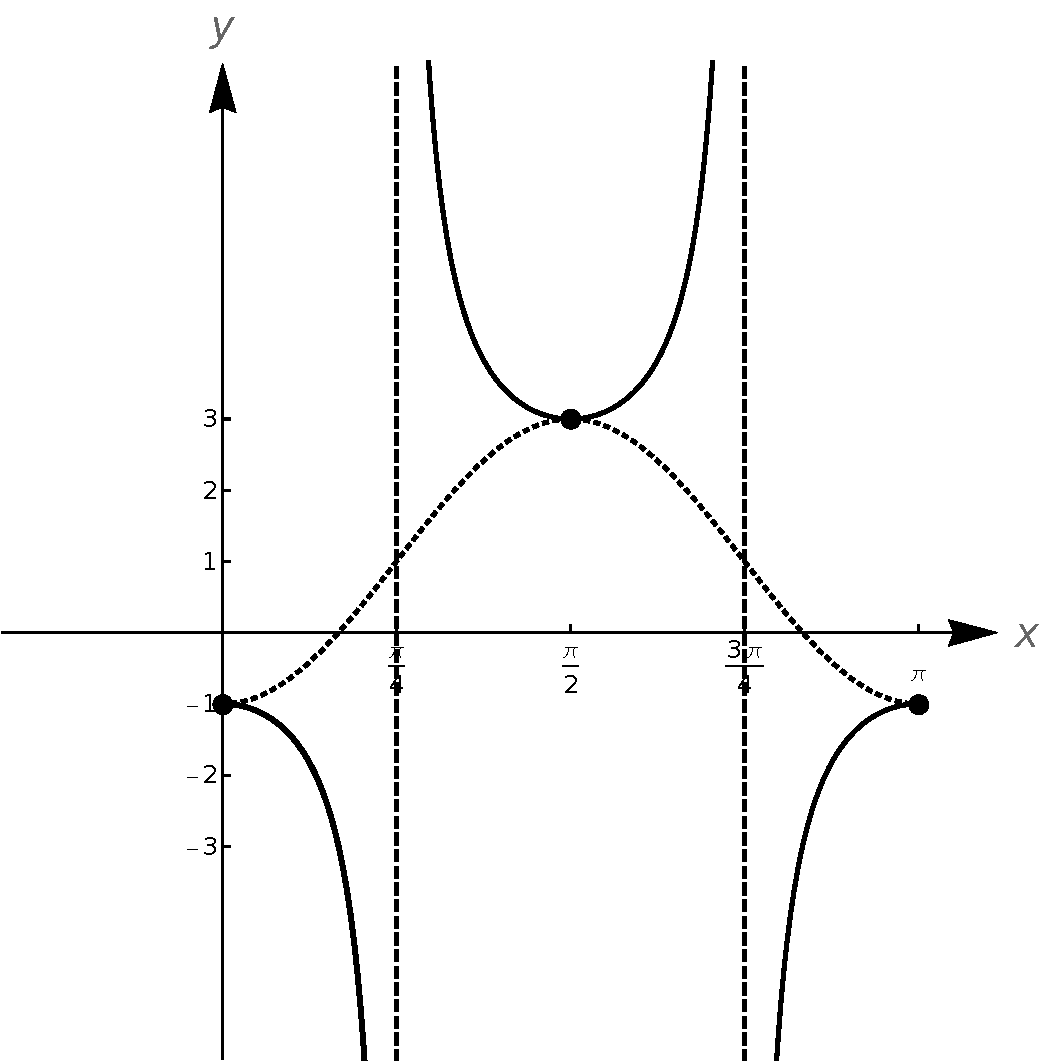
\includegraphics[width=0.45\textwidth]{fig_trans_25a}}
\hspace{0.1cm}
\subfigure[\label{fig_trans_25b}]{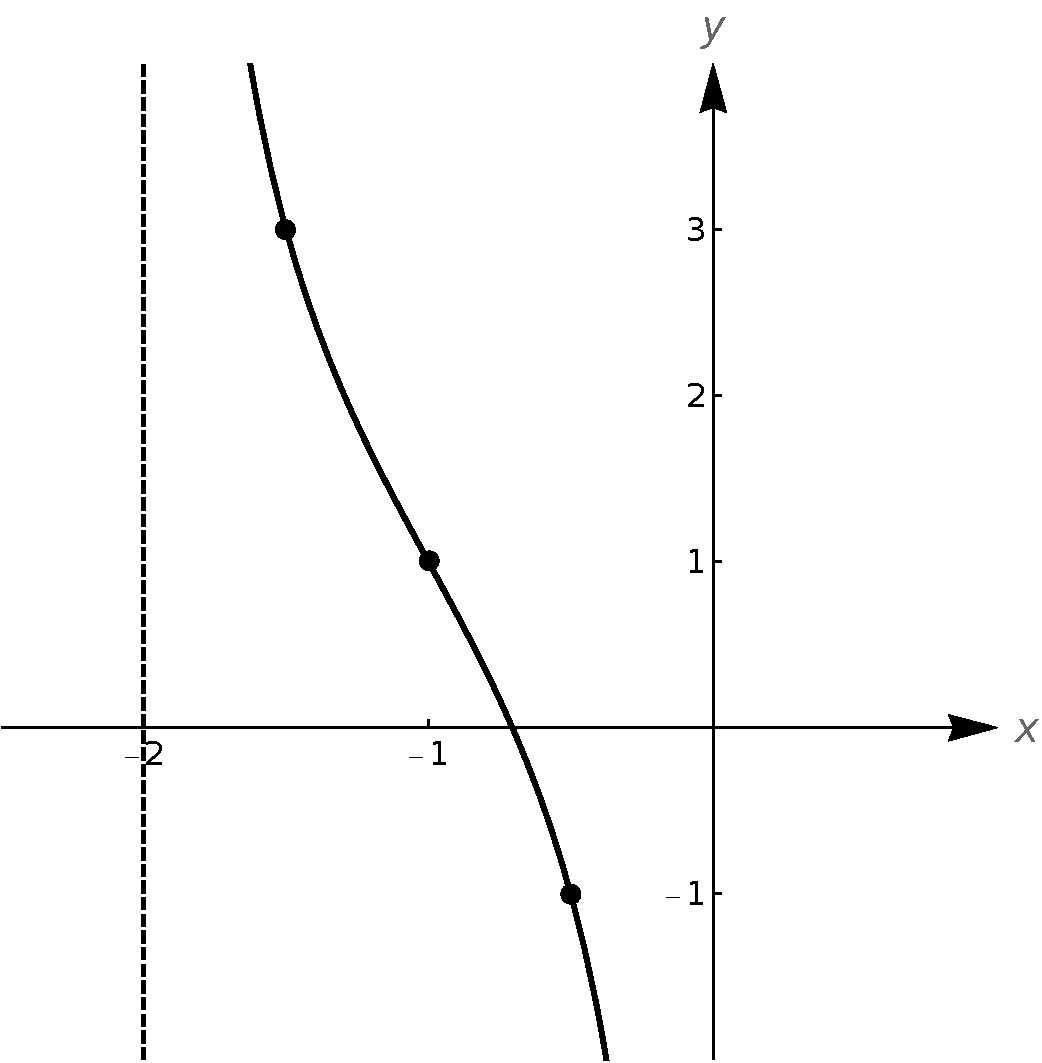
\includegraphics[width=0.45\textwidth]{fig_trans_25b}}
}
	\caption{One cycle of $y=1-2\sec(2x)$ (a) and $y=2\cot(\frac{\pi}{2}x+\pi)+1$ (b) over $[0,2\pi]$.}
\end{figure}


\end{example}


\ifcourse
\subsubsection{Applications}
Trigonometric functions are often used to solve problems that involve periodic behaviour, such as

\begin{itemize}
\item problems that involve circular movement on a repetitive nature;
\item problems involving repetitive motion, such as spring motion (Figure~\ref{fig_trans_26a}), oscillating waves and tides (Figure~\ref{fig_trans_26b});
\item problems involving environmental fluctuations (Figure~\ref{fig_trans_26c}). 
\end{itemize}


\begin{figure}
			\centering
%\raisebox{0.5cm}{
\centerline{
\subfigure[Motion of an object attached to a spring. \label{fig_trans_26a}]{\includegraphics[width=0.45\textwidth]{fig_trans_26a}}
\hspace{0.1cm}
\subfigure[Water height above sea level of the river Scheldt at the monitoring station Prosperpolder. \label{fig_trans_26b}]{\includegraphics[width=0.45\textwidth]{fig_trans_26b}}
}
\centerline{
\subfigure[Variation in annual cycle of river temperature at the Struma River in Bulgaria at the site of Boboshevo. \label{fig_trans_26c}]{\includegraphics[width=0.45\textwidth]{fig_trans_26c}}
}
	\caption{Applications of trigonometric functions illustrated.}
\end{figure}


\begin{example}
 According to the U.S. Naval Observatory website, the number of hours $H$ of daylight that Fairbanks, Alaska received on the 21st day of the $n$th month of 2009 is given below.  Here  $t = 1$ represents January 21, 2009, $t = 2$ represents February 21, 2009, and so on.  

\begin{center}
\noindent \begin{tabular}{p{1.5cm}|rrrrrrrrrrrr} \hline\hline
Month & 1 & 2 & 3 & 4 & 5 & 6 & 7 & 8 & 9 & 10 & 11 & 12\\ 
\hline 
Hours of Daylight & 5.8 & 9.3 & 12.4 & 15.9 & 19.4 & 21.8 & 19.4 & 15.6 & 12.4 & 9.1 & 5.6 & 3.3 \\ \hline\hline
\end{tabular}
\end{center}


\ifmathematica
Find a sinusoid that models these data and use Mathematica to graph your answer along with the data. 
\fi
\ifpython
Find a sinusoid that models these data and use Python to graph your answer along with the data. 
\fi

\xhrulefill{gray}{2.5pt}Solution \xhrulefill{gray}{2.5pt}
\ifmathematica
 To get a feel for the data, we first plot it using the Mathematica built-in function \lstinline{ListPlot}.
 The result is plotted in Figure~\ref{fig_trans_27}.
 \fi
 \ifpython
  To get a feel for the data, we first plot it using the Python built-in function \lstinline{scatter}.
 The result is plotted in Figure~\ref{fig_trans_27}.\fi

\begin{figure}[H]
	\begin{center}
			\includegraphics[width=0.5\textwidth]{fig_trans_27}
	\caption{Hours of daylight on the 21st day of the month of 2009 in Fairbanks, Alaska}
	\label{fig_trans_27}
	\end{center}
\end{figure}




We do our best to find the constants $A$, $\omega$, $\phi$ and $B$ so that  $H(t) = A\sin(\omega t + \phi) + B$ closely matches the data.  We first go after the vertical shift $B$ whose value determines the baseline.  In a typical sinusoid, the value of $B$ is the average of the maximum and minimum values.  So here we take $B = \frac{3.3+21.8}{2} = 12.55$.  Next is the amplitude $A$ which is the displacement from the baseline to the maximum (and minimum) values.  We find $A = 21.8 - 12.55 = 12.55 - 3.3 = 9.25$.  At this point, we have $H(t) = 9.25\sin(\omega t + \phi) + 12.55$.  Next, we go after the angular frequency $\omega$.  Since the data collected is over the span of a year (12 months), we take the period $T = 12$ months.  This means $\omega = \frac{2\pi}{T} = \frac{2\pi}{12} = \frac{\pi}{6}$.  The last quantity to find is the phase $\phi$. It is easy to find the phase shift $-\frac{\phi}{\omega}$.  Since we picked $A > 0$, the phase shift corresponds to the first value of $t$ with $H(t) = 12.55$ (the baseline value).  Here, we choose $t = 3$, since its corresponding $H$ value of $12.4$ is closer to  $12.55$ than the next value, $15.9$, which corresponds to $t=4$.  Hence, $-\frac{\phi}{\omega} = 3$, so $\phi = -3 \omega = -3 \left(\frac{\pi}{6}\right) = -\frac{\pi}{2}$.  We have 
$$H(t) = 9.25 \sin\left(\frac{\pi}{6} t - \frac{\pi}{2}\right) + 12.55,$$
whose graph is shown together with the data in Figure~\ref{fig_trans_28}. 

\begin{figure}[H]
	\begin{center}
			\includegraphics[width=0.5\textwidth]{fig_trans_28}
	\caption{Hours of daylight on the 21st day of the month of 2009 in Fairbanks, Alaska}
	\label{fig_trans_28}
	\end{center}
\end{figure}


\end{example}


\begin{remark}[Forgotten trigonometric functions]
In addition to the trigonometric functions we encountered in this chapter, there are a few functions that were common historically, but are nowadays sometimes forgotten, such as the chord, given by 
$$
\text{crd}(\theta) = 2\sin\left(\frac{\theta}{2}\right),
$$
the versine 
$$\text{versin}(\theta) = 1 - cos(\theta),
$$
and  the haversine 
$$
\text{haversin}(\theta) = \dfrac{1}{2}\text{versin}(\theta).
$$
Still these functions are used in several fields. For instance, one period  of a versine or haversine is commonly used in signal processing and control theory as the shape of a pulse.
\end{remark}

\fi

\ifcourse

\section{Inverse trigonometric functions}
\label{sec_inverse_trig}
In this section we concern ourselves with finding inverses of the trigonometric functions, which are also referred to as \textbf{arcus}, \textbf{antitrigonometric} or \textbf{cyclometric functions} (\textit{cyclometrische functies}).  Our immediate problem is that, owing to their periodic nature, none of the six trigoniometric functions is  injective. To remedy this, we restrict the domains of the circular functions in the same way we restricted the domain of the quadratic function in Example~\ref{inverserestrictionex} to obtain an injective function. 

\subsection{Inverse cosine and sine functions}
We first consider $f(x) = \cos(x)$. Choosing the interval $[0,\pi]$ allows us to keep the range as $[-1,1]$ as well as the properties of being smooth and continuous. Recall from Section~\ref{sec_inverse} that the inverse of a function $f$ is typically denoted $f^{-1}$.  For this reason, some textbooks use the notation $f^{-1}(x) = \cos^{-1}(x)$ for the inverse of $f(x) = \cos(x)$.  The obvious pitfall here is our convention of writing $(\cos(x))^2$ as $\cos^{2}(x)$, $(\cos(x))^3$ as $\cos^{3}(x)$ and so on.  It is far too easy to confuse $\cos^{-1}(x)$ with  $\frac{1}{\cos(x)} = \sec(x)$, so we will not use this notation.  Instead, we use the notation $f^{-1}(x) = \arccos(x)$, read \textbf{arccosine} (\textit{boogcosinus}) of $x$.  As a consequence of the imposed domain restriction, we have that
$$\cos(\arccos(x)) = x\,,$$
provided $-1 \leq x \leq 1$, and $$\arccos(\cos(x)) = x\,,$$
provided $0 \leq x \leq \pi$, which is important to keep in mind when solving equations involving (inverse) trigonometric functions. 



To understand the arc in arccosine, recall that an inverse function, by definition, reverses the process of the original function. The function $f(x) = \cos(x)$ takes a real number input $x$, associates it with the angle $\theta = x$ radians, and returns the value $\cos(\theta)$.  Digging deeper, we have that $\cos(\theta) = \cos(x)$ is the $x$-coordinate of the terminal point on the unit circle of an oriented arc of length $|x|$ whose initial point is $(1, 0)$.  Hence, we may view the inputs to $f(x) = \cos(x)$ as oriented arcs and the outputs as $x$-coordinates on the unit circle.  The function $f^{-1}$, then, would take $x$-coordinates on the unit circle and return oriented arcs, hence the arc in arccosine. In Figure~\ref{fig_trans_29} are the graphs of $f(x) = \cos(x)$ and $f^{-1}(x) = \arccos(x)$, where we obtain the latter from the former by reflecting it across the line $y=x$, in accordance with what we learned in Section~\ref{sec_inverse}. \index{arccosine ! graph}\index[aut]{arccosinus ! grafiek}\index[aut]{boogcosinus ! grafiek}

\begin{figure}[H]
	\centering
	%\raisebox{0.5cm}{
	\centerline{
		\includegraphics[width=0.4\textwidth]{fig_trans_29}
	}
	\caption{The graph of $y=\cos(x)$ for $x\in[0, \pi]$ (dashed) and $y=\arccos(x)$ for $x\in[-1, 1]$ (solid).}
	\label{fig_trans_29}
\end{figure}


We restrict $g(x) = \sin(x)$ in a similar manner, although the interval of choice is $\left[ -\frac{\pi}{2}, \frac{\pi}{2}\right]$ (Figure~\ref{fig_trans_30}). It should be no surprise that we call $g^{-1}(x) = \arcsin(x)$, which is read \textbf{arcsine} (\textit{boogsinus}) of $x$. From Figure~\ref{fig_trans_30}, we may infer that the arcsine is an odd function. Besides, due to the domain restriction, we have that $$\sin(\arcsin(x)) = x\,,$$
provided $-1 \leq x \leq 1$ and  $$\arcsin(\sin(x)) = x\,,$$
provided $-\frac{\pi}{2} \leq x \leq \frac{\pi}{2}$.   \index{arcsine ! graph} \index[aut]{arcsinus ! grafiek}\index[aut]{boogsinus ! grafiek}


\begin{figure}[H]
	\centering
	%\raisebox{0.5cm}{
	\centerline{
		\includegraphics[width=0.4\textwidth]{fig_trans_30}
	}
	\caption{The graph of $y=\sin(x)$ for $x\in\left[-\frac{\pi}{2}, \frac{\pi}{2}\right]$ (dashed) and $y=\arcsin(x)$ for $x\in[-1, 1]$ (solid).}
	\label{fig_trans_30}
\end{figure}


\begin{example}  \label{arccosinesineex} 
	Find the exact values of the following.
	
	\begin{multicols}{2}
		
		\begin{enumerate}
			
			\item $\arccos\left(\dfrac{1}{2}\right)$
			\item  $\arccos\left(-\dfrac{\sqrt{2}}{2}\right)$
			\item  $\arcsin\left(-\dfrac{1}{2}\right)$
			\item  $\arccos\left( \cos\left(\dfrac{\pi}{6}\right)\right)$
			\item  $\arccos\left( \cos\left(\dfrac{11\pi}{6}\right)\right)$
			\item  $\sin\left(\arccos\left(-\dfrac{3}{5}\right)\right)$
		\end{enumerate}
		
	\end{multicols}
	
	\xhrulefill{gray}{2.5pt}Solution \xhrulefill{gray}{2.5pt}
	
	\begin{enumerate}
		
		\item  To find $\arccos\left(\frac{1}{2}\right)$, we need to find the real number $x$ that lies between $0$ and $\pi$ for which it holds that $\cos(x) = \frac{1}{2}$. We know $x = \frac{\pi}{3}$ meets these criteria, so $\arccos\left(\frac{1}{2}\right)= \frac{\pi}{3}$.
		
		\item  The number $x = \arccos\left(-\frac{\sqrt{2}}{2}\right)$ lies in the interval $[0,\pi]$ with $\cos(x) = -\frac{\sqrt{2}}{2}$.  Our answer is $\arccos\left(-\frac{\sqrt{2}}{2}\right) = \frac{3\pi}{4}$.
		
		\item  To find  $\arcsin\left(-\frac{1}{2}\right)$, we seek the number $x$ in the interval $\left[-\frac{\pi}{2}, \frac{\pi}{2}\right]$ with $\sin(x) = -\frac{1}{2}$.  The answer is $x = -\frac{\pi}{6}$ so that $\arcsin\left(-\frac{1}{2}\right) = -\frac{\pi}{6}$.
		
		\item  Since $0 \leq \frac{\pi}{6} \leq \pi$, we simply have that $\arccos\left( \cos\left(\frac{\pi}{6}\right)\right) = \frac{\pi}{6}$.  However, in order to make sure we understand why this is the case, we can use the definition of arccosine.  Working from the inside out,  $\arccos\left( \cos\left(\frac{\pi}{6}\right)\right) = \arccos\left( \frac{\sqrt{3}}{2}\right)$.  Now, $\arccos\left( \frac{\sqrt{3}}{2}\right)$ is the real number $x$ with $0 \leq x \leq \pi$ and $\cos(x) = \frac{\sqrt{3}}{2}$.  We find $x = \frac{\pi}{6}$, so that  $\arccos\left( \cos\left(\frac{\pi}{6}\right)\right) = \frac{\pi}{6}$.
		
		\item Since $\frac{11\pi}{6}$ does not fall between $0$ and $\pi$, we are forced to work from the inside out starting with  $\arccos\left( \cos\left(\frac{11\pi}{6}\right)\right) = \arccos\left(\frac{\sqrt{3}}{2}\right)$.  From the previous problem, we know \\ $\arccos\left(\frac{\sqrt{3}}{2}\right) = \frac{\pi}{6}$.  Hence,  $\arccos\left( \cos\left(\frac{11\pi}{6}\right)\right) = \frac{\pi}{6}$.
		
		\item  We let $x = \arccos\left(-\frac{3}{5}\right)$ so that  $\cos(x) = -\frac{3}{5}$ for some $x$ where  $0 \leq x \leq \pi$.  Since $\cos(x) < 0$, we can narrow this down a bit and conclude that $\frac{\pi}{2} < x < \pi$, so that $x$ corresponds to an angle in Quadrant II. In terms of $x$, then, we need to find $\sin\left(\arccos\left(-\frac{3}{5}\right)\right) = \sin(x)$.  Using the Pythagorean identity, we get $\left(-\frac{3}{5}\right)^2 + \sin^{2}(x) = 1$ or $\sin(x) = \pm \frac{4}{5}$.  Since $x$ corresponds to a Quadrants II angle, we choose  $\sin(x) = \frac{4}{5}$.  Hence,  $\sin\left(\arccos\left(-\frac{3}{5}\right)\right) = \frac{4}{5}$.
		
	\end{enumerate}
\end{example}

Most of the common errors encountered in dealing with the inverse trigonometric functions come from the need to restrict the domains of the original functions so that they are injective.  One instance of this phenomenon is the fact that $\arccos\left( \cos\left(\frac{11\pi}{6}\right)\right) = \frac{\pi}{6}$ as opposed to $\frac{11\pi}{6}$. This is the exact same phenomenon discussed in Section~\ref{sec_inverse} when we saw  $\sqrt{(-2)^2} = 2$ as opposed to $-2$.   

\subsection{Inverse tangent and cotangent functions}
\ifcourse
	\checkoddpage
\marginpar{\ifoddpage\hspace*{-1.5cm}\else\hspace*{0.25cm}\fi\includegraphics[width=0.075\textwidth]{youtube}\\
\ifoddpage\hspace*{-1.75cm}\else\hspace*{0.1cm}\fi
\qrcode[height=1.75cm]{https://youtu.be/Idxeo49szW0}
%\includegraphics[width=0.1\textwidth]{arctan}
}
 \fi
The next pair of functions we  discuss are the inverses of tangent and cotangent, which are named \textbf{arctangent} (\textit{boogtangens}) and \textbf{arccotangent} (\textit{boogcotangens}), respectively.  First, we restrict \\ $f(x) = \tan(x)$ to its fundamental cycle on $\left.\right]-\frac{\pi}{2}, \frac{\pi}{2}\left[\right.$ to obtain $f^{-1}(x) = \arctan(x)$. Among other things, note that the vertical asymptotes $x = -\frac{\pi}{2}$ and $x = \frac{\pi}{2}$ of the graph of $f(x) = \tan(x)$ become the horizontal asymptotes $y = -\frac{\pi}{2}$ and $y = \frac{\pi}{2}$ of the graph of $f^{-1}(x) = \arctan(x)$ (Figure~\ref{fig_trans_31}).  \index{arctangent ! graph} \index[aut]{arctangens ! grafiek}\index[aut]{boogtangens ! grafiek}Observe that the arctangent is an odd function and due to the domain restrition that  $$\tan\left(\arctan(x)\right) = x\,,$$
for all real numbers $x$, whereas $$\arctan(\tan(x)) = x\,,$$ $-\frac{\pi}{2} < x < \frac{\pi}{2}$ only. 

\begin{figure}[h]
	\centering
	%\raisebox{0.5cm}{
	\centerline{
		\subfigure[]{\includegraphics[width=0.4\textwidth]{fig_trans_31a}}
		\hspace{0.1cm}
		\subfigure[]{\includegraphics[width=0.4\textwidth]{fig_trans_31b}}
	}
	\caption{One cycle of $y=\tan(x)$ (a) and $y=\arctan(x)$ (b).}
	\label{fig_trans_31}
\end{figure}


Next, we restrict $g(x) = \cot(x)$ to its fundamental cycle on $\left.\right]0,\pi\left[\right.$ to obtain $g^{-1}(x) = \mbox{arccot}(x)$.  Once again, the vertical asymptotes $x=0$ and $x=\pi$ of the graph of $g(x) = \cot(x)$ become the horizontal asymptotes $y = 0$ and $y = \pi$ of the graph of $g^{-1}(x) = \mbox{arccot}(x)$ (Figure~\ref{fig_trans_32}). Moreover, as a consequence of the imposed domain restriction, we have $$\cot\left(\mbox{arccot}(x)\right) = x\,,$$ for all real numbers $x$ and $$\mbox{arccot}(\cot(x)) = x\,,$$ provided $0 < x < \pi$ only. Finally, we also have that
$$
\arctan(x) = \mbox{arccot}\left(\frac{1}{x}\right)\,,
$$
for $x > 0$ and likewise
$$
\mbox{arccot}(x) =\arctan\left(\frac{1}{x}\right)\,,
$$
for $x > 0$.
\index{arccotangent ! graph} \index[aut]{arccotangens ! grafiek}\index[aut]{boogcotangens ! grafiek}

\begin{figure}[h]
	\centering
	%\raisebox{0.5cm}{
	\centerline{
		\subfigure[]{\includegraphics[width=0.4\textwidth]{fig_trans_32a}}
		\hspace{0.1cm}
		\subfigure[]{\includegraphics[width=0.4\textwidth]{fig_trans_32b}}
	}
	\caption{One cycle of $y=\cot(x)$ (a) and $y=\mbox{arccot}(x)$ (b).}
	\label{fig_trans_32}
\end{figure}

\begin{example}
	Rewrite the following as algebraic expressions of $x$ and state the domain on which the equivalence is valid.
	
	\begin{multicols}{2}
		
		\begin{enumerate}
			
			\item  $\tan(2 \arctan(x))$
			
			\item  $\cos(\mbox{arccot}(2x))$ 
			
		\end{enumerate}
		
	\end{multicols}
	
	\xhrulefill{gray}{2.5pt}Solution \xhrulefill{gray}{2.5pt}
	
	\begin{enumerate}
		
		\item If we let $t = \arctan(x)$, then $-\frac{\pi}{2} < t < \frac{\pi}{2}$ and $\tan(t) = x$.   We look for a way to express $\tan(2 \arctan(x)) = \tan(2t)$ in terms of $x$.  Before we get started using identities, we note that $\tan(2t)$ is undefined when $2t = \frac{\pi}{2} + \pi k$ for integers $k$.  Dividing both sides of this equation by $2$ tells us we need to exclude values of $t$ where $t = \frac{\pi}{4} + \frac{\pi}{2} k$, where $k$ is an integer.  The only members of this family which lie in $\left.\right]-\frac{\pi}{2}, \frac{\pi}{2}\left[\right.$ are $t = \pm \frac{\pi}{4}$, which means the values of $t$ under consideration are $\left.\right]-\frac{\pi}{2}, -\frac{\pi}{4}\left[\right. \cup \left.\right]-\frac{\pi}{4}, \frac{\pi}{4}\left[\right. \cup \left.\right]\frac{\pi}{4}, \frac{\pi}{2}\left[\right.$.  Returning to $\tan(2t)$, we note the double angle identity $\tan(2t) = \frac{2 \tan(t)}{1 - \tan^{2}(t)}$, is valid for all the values of $t$ under consideration, hence we get 
		$$
		\tan(2 \arctan(x)) = \tan(2t) = \frac{2 \tan(t)}{1 - \tan^{2}(t)}= \frac{2x}{1-x^2}\,.
		$$
		To find where this equivalence is valid we check back with our substitution $t = \arctan(x)$. Since the domain of $\arctan(x)$ is all real numbers, the only exclusions come from the values of $t$ we discarded earlier, $t = \pm \frac{\pi}{4}$.   Since $x =\tan(t)$, this means we exclude $x = \tan\left(\pm \frac{\pi}{4}\right) = \pm 1$.  Hence, the equivalence  $\tan(2 \arctan(x)) =  \frac{2x}{1-x^2}$ holds for all $x$ in $\mathbb{R}\setminus\{-1,1\}$.
		
		\item  To get started, we let $t = \mbox{arccot}(2x)$ so that  $\cot(t) = 2x$ where $0 < t < \pi$.  In terms of $t$, $\cos(\mbox{arccot}(2x)) = \cos(t)$, and our goal is to express the latter in terms of $x$.   Since $\cos(t)$ is always defined, there are no additional restrictions on $t$, so we can begin using identities to relate $\cot(t)$ to $\cos(t)$.  The identity $\cot(t) = \frac{\cos(t)}{\sin(t)}$ is valid for $t$ in $]0,\pi[$, so our strategy is to obtain $\sin(t)$ in terms of $x$, then write $\cos(t) = \cot(t) \sin(t)$.   The identity $1 + \cot^{2}(t) = \csc^{2}(t)$ holds for all $t$ in $]0,\pi[$ and relates $\cot(t)$ and $\csc(t) = \frac{1}{\sin(t)}$.  Substituting $\cot(t) =2x$, we get  $1 + (2x)^2 = \csc^{2}(t)$, or $\csc(t) =  \pm \sqrt{4x^2+1}$. Since $t$ is between $0$ and $\pi$, $\csc(t) > 0$, so $\csc(t) =\sqrt{4x^2+1}$ which gives $\sin(t) = \left(4x^2+1\right)^{-1/2}$. Hence, 
		$$
		\cos(\mbox{arccot}(2x)) = \cos(t) = \cot(t) \sin(t) = \frac{2x}{\sqrt{4x^2+1}}\,.
		$$
		Since $\mbox{arccot}(2x)$ is defined for all real numbers $x$ and we encountered no additional restrictions on $t$, we have  $\cos\left(\mbox{arccot}(2x)\right) = \frac{2x}{\sqrt{4x^2+1}}$ for all real numbers $x$. 
		
	\end{enumerate}
\end{example}
\fi


\ifvc

\section{Inverse trigonometric functions}
\label{sec_inverse_trig}
In this section we concern ourselves with finding inverses of the trigonometric functions, which are also referred to as \textbf{arcus}, \textbf{antitrigonometric} or \textbf{cyclometric functions} (\textit{cyclometrische functies}).  Our immediate problem is that, owing to their periodic nature, none of the six trigoniometric functions is  injective. To remedy this, we restrict the domains of the circular functions in the same way we restricted the domain of the quadratic function in Example~\ref{inverserestrictionex} to obtain an injective function. 

\subsection{Inverse cosine and sine functions}
We first consider $f(x) = \cos(x)$. Choosing the interval $[0,\pi]$ allows us to keep the range as $[-1,1]$ as well as the properties of being smooth and continuous. Recall from Section~\ref{sec_inverse} that the inverse of a function $f$ is typically denoted $f^{-1}$.  For this reason, some textbooks use the notation $f^{-1}(x) = \cos^{-1}(x)$ for the inverse of $f(x) = \cos(x)$.  The obvious pitfall here is our convention of writing $(\cos(x))^2$ as $\cos^{2}(x)$, $(\cos(x))^3$ as $\cos^{3}(x)$ and so on.  It is far too easy to confuse $\cos^{-1}(x)$ with  $\frac{1}{\cos(x)} = \sec(x)$, so we will not use this notation.  Instead, we use the notation $f^{-1}(x) = \arccos(x)$, read \textbf{arccosine} (\textit{boogcosinus}) of $x$.  As a consequence of the imposed domain restriction, we have that
 $\cos(\arccos(x)) = x$,  provided $-1 \leq x \leq 1$, and $\arccos(\cos(x)) = x$, provided $0 \leq x \leq \pi$, which is important to keep in mind when solving equations involving (inverse) trigonometric functions. 
 


To understand the arc in arccosine, recall that an inverse function, by definition, reverses the process of the original function. The function $f(x) = \cos(x)$ takes a real number input $x$, associates it with the angle $\theta = x$ radians, and returns the value $\cos(\theta)$.  Digging deeper, we have that $\cos(\theta) = \cos(x)$ is the $x$-coordinate of the terminal point on the unit circle of an oriented arc of length $|x|$ whose initial point is $(1, 0)$.  Hence, we may view the inputs to $f(x) = \cos(x)$ as oriented arcs and the outputs as $x$-coordinates on the unit circle.  The function $f^{-1}$, then, would take $x$-coordinates on the unit circle and return oriented arcs, hence the arc in arccosine. In Figure~\ref{fig_trans_33} are the graphs of $f(x) = \cos(x)$ and $f^{-1}(x) = \arccos(x)$, where we obtain the latter from the former by reflecting it across the line $y=x$, in accordance with what we learned in Section~\ref{sec_inverse}. \index{arccosine ! graph}\index[aut]{arccosinus ! grafiek}\index[aut]{boogcosinus ! grafiek}

\begin{figure}[H]
			\centering
%\raisebox{0.5cm}{
\centerline{
\includegraphics[width=0.4\textwidth]{fig_trans_33}
}
	\caption{The graph of $y=\cos(x)$ for $x\in[0, \pi]$ (grey) and $y=\arccos(x)$ for $x\in[-1, 1]$ (black).}
\label{fig_trans_33}
\end{figure}


We restrict $g(x) = \sin(x)$ in a similar manner, although the interval of choice is $\left[ -\frac{\pi}{2}, \frac{\pi}{2}\right]$ (Figure~\ref{fig_trans_34}). It should be no surprise that we call $g^{-1}(x) = \arcsin(x)$, which is read \textbf{arcsine} (\textit{boogsinus}) of $x$. From Figure~\ref{fig_trans_34}, we may infer that the arcsine is an odd function. Besides, due to the domain restriction, we have that $\sin(\arcsin(x)) = x$,  provided $-1 \leq x \leq 1$ and  $\arcsin(\sin(x)) = x$, provided $-\frac{\pi}{2} \leq x \leq \frac{\pi}{2}$.   \index{arcsine ! graph} \index[aut]{arcsinus ! grafiek}\index[aut]{boogsinus ! grafiek}


\begin{figure}[H]
			\centering
%\raisebox{0.5cm}{
\centerline{
\includegraphics[width=0.4\textwidth]{fig_trans_34}
}
	\caption{The graph of $y=\sin(x)$ for $x\in\left[-\frac{\pi}{2}, \frac{\pi}{2}\right]$ (grey) and $y=\arcsin(x)$ for $x\in[-1, 1]$ (black).}
\label{fig_trans_34}
\end{figure}


\begin{example}  \label{arccosinesineex} 
 Find the exact values of the following.

\begin{multicols}{2}

\begin{enumerate}

\item $\arccos\left(\frac{1}{2}\right)$
\item  $\arccos\left(-\frac{\sqrt{2}}{2}\right)$
\item  $\arcsin\left(-\frac{1}{2}\right)$
\item  $\arccos\left( \cos\left(\frac{\pi}{6}\right)\right)$
\item  $\arccos\left( \cos\left(\frac{11\pi}{6}\right)\right)$
\item  $\sin\left(\arccos\left(-\frac{3}{5}\right)\right)$
\end{enumerate}

\end{multicols}

\xhrulefill{gray}{2.5pt}Solution \xhrulefill{gray}{2.5pt}

\begin{enumerate}

\item  To find $\arccos\left(\frac{1}{2}\right)$, we need to find the real number $x$ that lies between $0$ and $\pi$ for which it holds that $\cos(x) = \frac{1}{2}$. We know $x = \frac{\pi}{3}$ meets these criteria, so $\arccos\left(\frac{1}{2}\right)= \frac{\pi}{3}$.

\item  The number $x = \arccos\left(-\frac{\sqrt{2}}{2}\right)$ lies in the interval $[0,\pi]$ with $\cos(x) = -\frac{\sqrt{2}}{2}$.  Our answer is $\arccos\left(-\frac{\sqrt{2}}{2}\right) = \frac{3\pi}{4}$.

\item  To find  $\arcsin\left(-\frac{1}{2}\right)$, we seek the number $x$ in the interval $\left[-\frac{\pi}{2}, \frac{\pi}{2}\right]$ with $\sin(x) = -\frac{1}{2}$.  The answer is $x = -\frac{\pi}{6}$ so that $\arcsin\left(-\frac{1}{2}\right) = -\frac{\pi}{6}$.

\item  Since $0 \leq \frac{\pi}{6} \leq \pi$, we simply have that $\arccos\left( \cos\left(\frac{\pi}{6}\right)\right) = \frac{\pi}{6}$.  However, in order to make sure we understand why this is the case, we can use the definition of arccosine.  Working from the inside out,  $\arccos\left( \cos\left(\frac{\pi}{6}\right)\right) = \arccos\left( \frac{\sqrt{3}}{2}\right)$.  Now, $\arccos\left( \frac{\sqrt{3}}{2}\right)$ is the real number $x$ with $0 \leq x \leq \pi$ and $\cos(x) = \frac{\sqrt{3}}{2}$.  We find $x = \frac{\pi}{6}$, so that  $\arccos\left( \cos\left(\frac{\pi}{6}\right)\right) = \frac{\pi}{6}$.

\item Since $\frac{11\pi}{6}$ does not fall between $0$ and $\pi$, we are forced to work from the inside out starting with  $\arccos\left( \cos\left(\frac{11\pi}{6}\right)\right) = \arccos\left(\frac{\sqrt{3}}{2}\right)$.  From the previous problem, we know \\ $\arccos\left(\frac{\sqrt{3}}{2}\right) = \frac{\pi}{6}$.  Hence,  $\arccos\left( \cos\left(\frac{11\pi}{6}\right)\right) = \frac{\pi}{6}$.

\item  We let $x = \arccos\left(-\frac{3}{5}\right)$ so that  $\cos(x) = -\frac{3}{5}$ for some $x$ where  $0 \leq x \leq \pi$.  Since $\cos(x) < 0$, we can narrow this down a bit and conclude that $\frac{\pi}{2} < x < \pi$, so that $x$ corresponds to an angle in Quadrant II. In terms of $x$, then, we need to find $\sin\left(\arccos\left(-\frac{3}{5}\right)\right) = \sin(x)$.  Using the Pythagorean identity, we get $\left(-\frac{3}{5}\right)^2 + \sin^{2}(x) = 1$ or $\sin(x) = \pm \frac{4}{5}$.  Since $x$ corresponds to a Quadrants II angle, we choose  $\sin(x) = \frac{4}{5}$.  Hence,  $\sin\left(\arccos\left(-\frac{3}{5}\right)\right) = \frac{4}{5}$.

\end{enumerate}
\end{example}

 Most of the common errors encountered in dealing with the inverse trigonometric functions come from the need to restrict the domains of the original functions so that they are injective.  One instance of this phenomenon is the fact that $\arccos\left( \cos\left(\frac{11\pi}{6}\right)\right) = \frac{\pi}{6}$ as opposed to $\frac{11\pi}{6}$. This is the exact same phenomenon discussed in Section~\ref{sec_inverse} when we saw  $\sqrt{(-2)^2} = 2$ as opposed to $-2$.   

\subsection{Inverse tangent and cotangent functions}
The next pair of functions we  discuss are the inverses of tangent and cotangent, which are named \textbf{arctangent} (\textit{boogtangens}) and \textbf{arccotangent} (\textit{boogcotangens}), respectively.  First, we restrict \\ $f(x) = \tan(x)$ to its fundamental cycle on $\left.\right]-\frac{\pi}{2}, \frac{\pi}{2}\left[\right.$ to obtain $f^{-1}(x) = \arctan(x)$. Among other things, note that the vertical asymptotes $x = -\frac{\pi}{2}$ and $x = \frac{\pi}{2}$ of the graph of $f(x) = \tan(x)$ become the horizontal asymptotes $y = -\frac{\pi}{2}$ and $y = \frac{\pi}{2}$ of the graph of $f^{-1}(x) = \arctan(x)$ (Figure~\ref{fig_trans_35}).  \index{arctangent ! graph} \index[aut]{arctangens ! grafiek}\index[aut]{boogtangens ! grafiek}Observe that the arctangent is an odd function and due to the domain restrition that  $\tan\left(\arctan(x)\right) = x$, for all real numbers $x$, whereas $\arctan(\tan(x)) = x$, provided $-\frac{\pi}{2} < x < \frac{\pi}{2}$ only. 

\begin{figure}[h]
			\centering
%\raisebox{0.5cm}{
\centerline{
\subfigure[]{\includegraphics[width=0.4\textwidth]{fig_trans_35a}}
\hspace{0.1cm}
\subfigure[]{\includegraphics[width=0.4\textwidth]{fig_trans_35b}}
}
	\caption{One cycle of $y=\tan(x)$ (a) and $y=\arctan(x)$ (b).}
	\label{fig_trans_35}
\end{figure}


Next, we restrict $g(x) = \cot(x)$ to its fundamental cycle on $\left.\right]0,\pi\left[\right.$ to obtain $g^{-1}(x) = \mbox{arccot}(x)$.  Once again, the vertical asymptotes $x=0$ and $x=\pi$ of the graph of $g(x) = \cot(x)$ become the horizontal asymptotes $y = 0$ and $y = \pi$ of the graph of $g^{-1}(x) = \mbox{arccot}(x)$ (Figure~\ref{fig_trans_36}). Moreover, as a consequence of the imposed domain restriction, we have $\cot\left(\mbox{arccot}(x)\right) = x$, for all real numbers $x$ and $\mbox{arccot}(\cot(x)) = x$, provided $0 < x < \pi$ only. Finally, we also have that
$$
\arctan(x) = \mbox{arccot}\left(\frac{1}{x}\right)\,,
$$
 for $x > 0$ and likewise
$$
\mbox{arccot}(x) =\arctan\left(\frac{1}{x}\right)\,,
$$
for $x > 0$.
 \index{arccotangent ! graph} \index[aut]{arccotangens ! grafiek}\index[aut]{boogcotangens ! grafiek}

\begin{figure}[h]
			\centering
%\raisebox{0.5cm}{
\centerline{
\subfigure[]{\includegraphics[width=0.4\textwidth]{fig_trans_36a}}
\hspace{0.1cm}
\subfigure[]{\includegraphics[width=0.4\textwidth]{fig_trans_36b}}
}
	\caption{One cycle of $y=\cot(x)$ (a) and $y=\mbox{arccot}(x)$ (b).}
	\label{fig_trans_36}
\end{figure}

\begin{example}
 Rewrite the following as algebraic expressions of $x$ and state the domain on which the equivalence is valid.

\begin{multicols}{2}

\begin{enumerate}

\item  $\tan(2 \arctan(x))$

\item  $\cos(\mbox{arccot}(2x))$ 

\end{enumerate}

\end{multicols}

\xhrulefill{gray}{2.5pt}Solution \xhrulefill{gray}{2.5pt}

\begin{enumerate}

\item If we let $t = \arctan(x)$, then $-\frac{\pi}{2} < t < \frac{\pi}{2}$ and $\tan(t) = x$.   We look for a way to express $\tan(2 \arctan(x)) = \tan(2t)$ in terms of $x$.  Before we get started using identities, we note that $\tan(2t)$ is undefined when $2t = \frac{\pi}{2} + \pi k$ for integers $k$.  Dividing both sides of this equation by $2$ tells us we need to exclude values of $t$ where $t = \frac{\pi}{4} + \frac{\pi}{2} k$, where $k$ is an integer.  The only members of this family which lie in $\left.\right]-\frac{\pi}{2}, \frac{\pi}{2}\left[\right.$ are $t = \pm \frac{\pi}{4}$, which means the values of $t$ under consideration are $\left.\right]-\frac{\pi}{2}, -\frac{\pi}{4}\left[\right. \cup \left.\right]-\frac{\pi}{4}, \frac{\pi}{4}\left[\right. \cup \left.\right]\frac{\pi}{4}, \frac{\pi}{2}\left[\right.$.  Returning to $\arctan(2t)$, we note the double angle identity $\tan(2t) = \frac{2 \tan(t)}{1 - \tan^{2}(t)}$, is valid for all the values of $t$ under consideration, hence we get 
$$
\tan(2 \arctan(x)) = \tan(2t) = \frac{2 \tan(t)}{1 - \tan^{2}(t)}= \frac{2x}{1-x^2}\,.
$$
To find where this equivalence is valid we check back with our substitution $t = \arctan(x)$. Since the domain of $\arctan(x)$ is all real numbers, the only exclusions come from the values of $t$ we discarded earlier, $t = \pm \frac{\pi}{4}$.   Since $x =\tan(t)$, this means we exclude $x = \tan\left(\pm \frac{\pi}{4}\right) = \pm 1$.  Hence, the equivalence  $\tan(2 \arctan(x)) =  \frac{2x}{1-x^2}$ holds for all $x$ in $\mathbb{R}\setminus\{-1,1\}$.

\item  To get started, we let $t = \mbox{arccot}(2x)$ so that  $\cot(t) = 2x$ where $0 < t < \pi$.  In terms of $t$, $\cos(\mbox{arccot}(2x)) = \cos(t)$, and our goal is to express the latter in terms of $x$.   Since $\cos(t)$ is always defined, there are no additional restrictions on $t$, so we can begin using identities to relate $\cot(t)$ to $\cos(t)$.  The identity $\cot(t) = \frac{\cos(t)}{\sin(t)}$ is valid for $t$ in $]0,\pi[$, so our strategy is to obtain $\sin(t)$ in terms of $x$, then write $\cos(t) = \cot(t) \sin(t)$.   The identity $1 + \cot^{2}(t) = \csc^{2}(t)$ holds for all $t$ in $]0,\pi[$ and relates $\cot(t)$ and $\csc(t) = \frac{1}{\sin(t)}$.  Substituting $\cot(t) =2x$, we get  $1 + (2x)^2 = \csc^{2}(t)$, or $\csc(t) =  \pm \sqrt{4x^2+1}$. Since $t$ is between $0$ and $\pi$, $\csc(t) > 0$, so $\csc(t) =\sqrt{4x^2+1}$ which gives $\sin(t) = \frac{1}{\sqrt{4x^2+1}}$. Hence, 
$$
\cos(\mbox{arccot}(2x)) = \cos(t) = \cot(t) \sin(t) = \frac{2x}{\sqrt{4x^2+1}}\,.
$$
Since $\mbox{arccot}(2x)$ is defined for all real numbers $x$ and we encountered no additional restrictions on $t$, we have  $\cos\left(\mbox{arccot}(2x)\right) = \frac{2x}{\sqrt{4x^2+1}}$ for all real numbers $x$. 

\end{enumerate}
\end{example}
\fi


\ifcourse
\ifcalculus
For comprehensiveness, Table~\ref{tab_res_tri} lists the domain restrictions and corresponding range of the trigonometric and inverse trigonometric functions that will be used throughout the remainder of this course.


\begin{table}[h]
\begin{tabular}{c|cc}
Function & Domain & Range \\ \hline\hline
\rule{0pt}{12pt} $\sin (x)$ & $[-\pi/2, \pi/2]$ & $[-1,1]$\\
\rule{0pt}{12pt}$\cos (x)$ & $[0,\pi]$ & $[-1,1]$ \\
\rule{0pt}{12pt}$\tan (x)$ & $\left.\right]-\pi/2,\pi/2\left.\right[$ & $\left.\right]-\infty,+\infty\left.\right[$	\\
\rule{0pt}{12pt}$\cot (x)$ & $\left.\right]0,\pi\left.\right[$ & $\left.\right]-\infty,+\infty\left.\right[$\\[0.1cm] \hline
$\arcsin (x)$ & $[-1,1]$ & $[-\pi/2, \pi/2]$ \\[0.1cm]
$\arccos (x) $ & $[-1,1]$ & $[0,\pi]$\\[0.1cm]
$\arctan (x) $ & $\left.\right]-\infty,+\infty\left.\right[$ & $\left.\right]-\pi/2,\pi/2\left.\right[$\\[0.1cm]
$\arccot (x) $ &  $ \left.\right]-\infty,+\infty\left.\right[$ & $\left.\right]0,\pi\left.\right[$	\\[0.1cm]\hline\hline
\end{tabular}
\caption{Domains and ranges of the trigonometric and inverse trigonometric functions.}\label{tab_res_tri}
\end{table}
\fi 
\fi


\ifvc
For comprehensiveness, Table~\ref{tab_res_tri} lists the domain restrictions and corresponding range of the trigonometric and inverse trigonometric functions that will be used throughout the remainder of this course.


\begin{table}[h]
	\begin{tabular}{c|cc}
		Function & Domain & Range \\ \hline\hline
		\rule{0pt}{12pt} $\sin (x)$ & $[-\pi/2, \pi/2]$ & $[-1,1]$\\
		\rule{0pt}{12pt}$\cos (x)$ & $[0,\pi]$ & $[-1,1]$ \\
		\rule{0pt}{12pt}$\tan (x)$ & $\left.\right]-\pi/2,\pi/2\left.\right[$ & $\left.\right]-\infty,+\infty\left.\right[$	\\
		\rule{0pt}{12pt}$\cot (x)$ & $\left.\right]0,\pi\left.\right[$ & $\left.\right]-\infty,+\infty\left.\right[$\\[0.1cm] \hline
		$\arcsin (x)$ & $[-1,1]$ & $[-\pi/2, \pi/2]$ \\[0.1cm]
		$\arccos (x) $ & $[-1,1]$ & $[0,\pi]$\\[0.1cm]
		$\arctan (x) $ & $\left.\right]-\infty,+\infty\left.\right[$ & $\left.\right]-\pi/2,\pi/2\left.\right[$\\[0.1cm]
		$\arccot (x) $ &  $ \left.\right]-\infty,+\infty\left.\right[$ & $\left.\right]0,\pi\left.\right[$	\\[0.1cm]\hline\hline
	\end{tabular}
	\caption{Domains and ranges of the trigonometric and inverse trigonometric functions.}\label{tab_res_tri}
\end{table} 
\fi


\ifcourse
\ifanalysis
%\subsection{Inverse secant and cosecant functions}
%
%%The last two functions to invert are secant and cosecant.  A portion of each of their graphs is shown in Figure~\ref{fig_trans_23c} and \ref{fig_trans_23d}, respectively with the fundamental cycles highlighted. It is clear from the graph of secant that we cannot find one single continuous piece of its graph which covers its entire range of $\left.\right]-\infty, -1] \cup [1, +\infty\left[\right.$ and restricts the domain of the function so that it is one-to-one.  The same is true for cosecant.  Thus in order to define the \textbf{arcsecant} (\textit{boogsecans}) and \textbf{arccosecant} (\textit{boogcosecans}) functions, we must settle for a piecewise approach wherein we choose one piece to cover the top of the range, namely  $[1, +\infty\left[\right.$, and another piece to cover the bottom, namely $\left.\right]-\infty, -1]$.  There are two generally accepted ways make these choices which restrict the domains of these functions so that they are one-to-one.  One approach simplifies the trigonometry associated with the inverse functions, but complicates the calculus;  the other makes the calculus easier, but the trigonometry less so.
%%\index{arcsecant} \index{arccosecant}
%%\index[aut]{boogsecans} \index[aut]{boogcosecans}
%
%
%
%
%%\subsubsection{Trigonometry friendly approach}
%%In this subsection, we restrict the secant and cosecant functions to coincide with the restrictions on cosine and sine, respectively.  For $f(x) = \sec(x)$, we restrict the domain to $\left[\right.0, \frac{\pi}{2}\left[\right. \cup \left.\right] \frac{\pi}{2}, \pi\left.\right]$ and we restrict $g(x) = \csc(x)$ to $\left[\right.-\frac{\pi}{2}, 0\left[\right. \cup \left.\right]0,  \frac{\pi}{2}\left.\right]$ (Figure~\ref{fig_trans_30}). Note that for both arcsecant and arccosecant, the domain is $\left.\right]-\infty, -1] \cup [1, +\infty\left[\right.$, or equivalently $\left\{ x : |x| \geq 1\right\}$.
%%\index{arccosecant ! graph} \index{arcsecant ! graph} \index[aut]{arcsecans ! grafiek}\index[aut]{boogsecans ! grafiek} \index[aut]{arccosecans ! grafiek}\index[aut]{boogcosecans ! grafiek}
%
%
%%\begin{figure}
%%			\centering
%%\raisebox{0.5cm}{
%%\centerline{
%%\subfigure[]{\includegraphics[width=0.45\textwidth]{fig_trans_30a}}
%%\hspace{0.1cm}
%%\subfigure[]{\includegraphics[width=0.45\textwidth]{fig_trans_30b}}
%%}
%%\centerline{
%%\subfigure[]{\includegraphics[width=0.45\textwidth]{fig_trans_30c}}
%%\hspace{0.1cm}
%%\subfigure[]{\includegraphics[width=0.45\textwidth]{fig_trans_30d}}
%%}
%%	\caption{The graph of $y=\sec(x)$ (a),  $y=\mbox{arcsec}(x)$ (b), $y=\csc(x)$ (c) and  $y=\mbox{arccsc}(x)$ (d) in the trigonometry-friendly approach.}
%%	\label{fig_trans_30}
%%\end{figure}
%
%
%%Under this choice of domain restriction, we find
%%\begin{itemize}
%%\item $\sec\left(\mbox{arcsec}(x)\right) = x$, provided $|x| \geq 1$,
%
%%\item  $\mbox{arcsec}(\sec(x)) = x$, provided $0 \leq x < \dfrac{\pi}{2}$ or $\dfrac{\pi}{2} < x \leq \pi$,
%
%%\item $\csc\left(\mbox{arccsc}(x)\right) = x$, provided $|x| \geq 1$,
%
%%\item  $\mbox{arccsc}(\csc(x)) = x$, provided $-\dfrac{\pi}{2} \leq x < 0$ or $0 < x \leq \dfrac{\pi}{2}$.
%%\end{itemize}
%%Besides, the arccosecant is odd, and it holds that
%%\begin{equation}
% %\mbox{arcsec}(x) = \arccos\left(\frac{1}{x}\right)\,,
%%\label{arcseccos1}
%%\end{equation}
% %provided $|x| \geq 1$ and
%%\begin{equation}
%%\mbox{arccsc}(x) = \arcsin\left(\frac{1}{x}\right)\,.
%%\label{arccsccos1}
%%\end{equation}
%
%
%
%
%
%%\subsubsection{Calculus friendly approach}
%%Here we adopt an alternative domain restriction for the secant and cosecant functions, which, however is advantageous from a calculus point of view. More precisely, we restrict $f(x) = \sec(x)$ to $\left[\right.0, \frac{\pi}{2}\left[\right. \cup \left[\right.\pi, \frac{3\pi}{2}\left[\right.$ and we restrict $g(x) = \csc(x)$ to $\left.\right]0, \frac{\pi}{2}\left.\right] \cup \left.\right] \pi, \frac{3\pi}{2}\left.\right]$ (Figure~\ref{fig_trans_31}).  \index{arccosecant ! graph} \index[aut]{arcsecans ! grafiek}\index[aut]{boogsecans ! grafiek} \index[aut]{arccosecans ! grafiek}\index[aut]{boogcosecans ! grafiek}
%%\index{arcsecant ! graph}
%
%%Under this choice of domain restriction, we find
%%\begin{itemize}
%%\item  $\sec\left(\mbox{arcsec}(x)\right) = x$, provided $|x| \geq 1$,
%
%%\item  $\mbox{arcsec}(\sec(x)) = x$, provided $0 \leq x < \frac{\pi}{2}$ or $ \pi \leq  x < \frac{3\pi}{2}$,
%
%
%%\item  $\csc\left(\mbox{arccsc}(x)\right) = x$, provided $|x| \geq 1$,
%
%%\item  $\mbox{arccsc}(\csc(x)) = x$, provided $0 < x \leq \frac{\pi}{2}$ or $\pi < x \leq \frac{3\pi}{2}$.
%%\end{itemize}
%%Besides, it holds that
%%\begin{equation}
%%\mbox{arcsec}(x) = \arccos\left(\frac{1}{x}\right)\,,
%%\label{arcseccos2}
%%\end{equation}
%%for $x \geq 1$, and
%%\begin{equation}
%%\mbox{arccsc}(x) = \arcsin\left(\frac{1}{x}\right)\,.
%%\label{arccsccos2}
%%\end{equation}
%%for $x \geq 1$ only.
%
%%\begin{figure}
%%			\centering
%%\raisebox{0.5cm}{
%%\centerline{
%%\subfigure[]{\includegraphics[width=0.45\textwidth]{fig_trans_31a}}
%%\hspace{0.1cm}
%%\subfigure[]{\includegraphics[width=0.45\textwidth]{fig_trans_31b}}
%%}
%%\centerline{
%%\subfigure[]{\includegraphics[width=0.45\textwidth]{fig_trans_31c}}
%%\hspace{0.1cm}
%%\subfigure[]{\includegraphics[width=0.45\textwidth]{fig_trans_31d}}
%%}
%%	\caption{The graph of $y=\sec(x)$ (a),  $y=\mbox{arcsec}(x)$ (b), $y=\csc(x)$ (c) and  $y=\mbox{arccsc}(x)$ (d) in the calculus-friendly approach.}
%	%\label{fig_trans_31}
%%\end{figure}
%
%%\begin{example}
%%Adopting the definitions of the arcsecant and arccosecant according to the trigonometry (A) and calculus-friendly (B) approach, find the exact values of
%
%%\begin{multicols}{2}
%
%%\begin{enumerate}
%
%%\item $\mbox{arcsec}(2),$
%
%%\item  $\mbox{arccsc}(-2),$
%
%%\item  $\mbox{arcsec}\left( \sec\left( \dfrac{5\pi}{4} \right) \right),$
%
%%\item  $\cot\left(\mbox{arccsc}\left(-3\right)\right).$
%
%%\end{enumerate}
%
%%\end{multicols}
%
%
%%\xhrulefill{gray}{2.5pt}Solution \xhrulefill{gray}{2.5pt}
%
%%\begin{enumerate}
%
%%\item[(A)]
%
%%\begin{enumerate}
%
%%\item[1.] Using Equation~\eqref{arcseccos1}, we have $\mbox{arcsec}(2) = \arccos\left(\frac{1}{2}\right) = \frac{\pi}{3}$.
%
%%\item[2.]  Now Equation~\eqref{arccsccos1} comes to our aid giving $\mbox{arccsc}(-2) = \arcsin\left(-\frac{1}{2}\right) = -\frac{\pi}{6}$.
%
%
%%\item[3.]  Since $\frac{5\pi}{4}$ does not fall between $0$ and $\frac{\pi}{2}$ or $\frac{\pi}{2}$ and $\pi$, we have to work inside out which yields  $$\mbox{arcsec}\left( \sec\left( \frac{5\pi}{4} \right) \right) = \mbox{arcsec}(-\sqrt{2}) = \arccos\left(-\frac{\sqrt{2}}{2}\right) = \frac{3\pi}{4}.$$
%
%%\item[4.]   One way to begin to simplify $\cot\left(\mbox{arccsc}\left(-3\right)\right)$ is to let $t = \mbox{arccsc}(-3)$.  Then,  $\csc(t) = -3$ and, since this is negative, we have that $t$ lies in the interval  $\left[\right. -\frac{\pi}{2},0\left[\right.$.  We are after $\cot\left(\mbox{arccsc}\left(-3\right)\right) = \cot(t)$, so we use the Pythagorean identity $1 + \cot^{2}(t) = \csc^{2}(t)$.  Substituting, we have $1 + \cot^{2}(t) = (-3)^2$, or $\cot(t) = \pm \sqrt{8} = \pm 2 \sqrt{2}$.  Since $-\frac{\pi}{2} \leq t < 0$, $\cot(t) < 0$, so we get  $\cot\left(\mbox{arccsc}\left(-3\right)\right) = -2\sqrt{2}$.
%
%%\end{enumerate}
%
%%\item[(B)] 
%
%%\begin{enumerate}
%
%%\item[1.]  Since $2 \geq 1$, we may invoke Equation~\eqref{arcseccos2}  to get $\mbox{arcsec}(2) = \arccos\left(\frac{1}{2}\right) = \frac{\pi}{3}$.
%
%%\item[2.]  Unfortunately, $-2$ is not greater to or equal to $1$, so we cannot use Equation~\eqref{arccsccos2} and convert this into an arcsine problem.  Instead, we appeal to the definition.  The real number $t = \mbox{arccsc}(-2)$ lies in $\left.\right]0,\frac{\pi}{2} \left.\right] \cup \left.\right]\pi, \frac{3\pi}{2}\left.\right]$ and satisfies $\csc(t) = -2$.  The $t$ we are after is $t = \frac{7\pi}{6}$, so $\mbox{arccsc}(-2) = \frac{7\pi}{6}$.
%
%%\item[3.]  Since $\frac{5\pi}{4}$ lies between $\pi$ and $\frac{3\pi}{2}$, we may simplify this to $\mbox{arcsec}\left( \sec\left( \frac{5\pi}{4} \right) \right) = \frac{5\pi}{4}$.  
%
%%\item[4.]  To simplify $\cot\left(\mbox{arccsc}\left(-3\right)\right)$ we let $t = \mbox{arccsc}\left(-3\right)$ so that  $\cot\left(\mbox{arccsc}\left(-3\right)\right) = \cot(t)$.  We know $\csc(t) = -3$, and since this is negative,  $t$ lies in $\left.\right] \pi, \frac{3\pi}{2}\left.\right]$.  Using the identity $1 + \cot^{2}(t) = \csc^{2}(t)$, we find $1 + \cot^{2}(t) = (-3)^2$ so that $\cot(t) = \pm \sqrt{8} = \pm 2 \sqrt{2}$.  Since $t$ is in the interval $\left.\right]\pi, \frac{3\pi}{2}\left.\right]$, we know $\cot(t) > 0$.  Our answer is $\cot\left(\mbox{arccsc}\left(-3\right)\right) = 2 \sqrt{2}$.
%
%%\end{enumerate}
%%\end{enumerate}
%%\end{example}




For comprehensiveness, Table~\ref{tab_res_tri} lists the domain restrictions and corresponding range of the trigonometric and inverse trigonometric functions that will be used throughout the remainder of this course.

\begin{table}
\begin{tabular}{c|cc}
Function & Domain & Range \\ \hline\hline
\rule{0pt}{12pt} $\sin (x)$ & $\mathbb{R}$ & $[-1,1]$\\
\rule{0pt}{12pt}$\cos (x)$ & $\mathbb{R}$ & $[-1,1]$ \\
\rule{0pt}{12pt}$\tan (x)$ & $\left.\right]-\frac{\pi}{2},\frac{\pi}{2}\left.\right[+k\pi$ & $\left.\right]-\infty,+\infty\left.\right[$	\\
\rule{0pt}{12pt}$\cot (x)$ & $\left.\right]0,\pi\left.\right[+k\pi$ & $\left.\right]-\infty,+\infty\left.\right[$\\
\rule{0pt}{12pt} $\csc (x)$ & $[-\frac{\pi}{2},0\left.\right[\cup \left.\right]0, \frac{\pi}{2}]+k\pi$ & $\left.\right]-\infty,-1]\cup [1,+\infty\left.\right[$\\
\rule{0pt}{12pt}$\sec (x)$ & $[0,\frac{\pi}{2}\left.\right[\cup \left.\right]\frac{\pi}{2},\pi]+k\pi$ & $\left.\right]-\infty,-1]\cup [1,+\infty\left.\right[$ \\[0.25cm] \hline
$\arcsin (x)$ & $[-1,1]$ & $[-\frac{\pi}{2}, \frac{\pi}{2}]$ \\[0.1cm]
$\arccos (x) $ & $[-1,1]$ & $[0,\pi]$\\[0.1cm]
$\arctan (x) $ & $\left.\right]-\infty,+\infty\left.\right[$ & $\left.\right]-\frac{\pi}{2},\frac{\pi}{2}\left.\right[$\\[0.1cm]
$\arccot (x) $ &  $ \left.\right]-\infty,+\infty\left.\right[$ & $\left.\right]0,\pi\left.\right[$	\\[0.1cm]
 $\arccsc (x)$ & $\left.\right]-\infty,-1]\cup [1,+\infty\left.\right]$ & $[-\frac{\pi}{2},0[\cup \left.\right]0, \frac{\pi}{2}]$  \\[0.1cm]
$\arcsec (x)$ & $\left.\right]-\infty,-1]\cup [1,+\infty\left.\right]$ & $[0,\frac{\pi}{2}\left.\right[\cup \left.\right]\frac{\pi}{2},\pi]$\\[0.1cm]
\hline\hline
\end{tabular}
\caption{Domains and ranges of the trigonometric and inverse trigonometric functions.}\label{tab_res_tri}
\end{table}


\fi
\fi



\ifvc
\subsection{Solving equations involving trigonometric functions}
We have already seen how to solve equations like $\tan(x) = -1$ for real numbers $x$ by appealing to the unit circle and relying on the fact that the answers corresponded to a set of common angles listed in Tables~\ref{tab_trans_1} and \ref{tab_trans_2}.  If, on the other hand, we had been asked to solve $\tan(x) = -2$ , we would have been hard-pressed to do so.  With the introduction of the inverse trigonometric functions, however, we are now in a position to solve these equations.  we will illustrate this functionality in the following example.

\begin{example}  \label{basicinverseeqns}  Solve the following equations.

\begin{multicols}{2}

\begin{enumerate}

\item  $\sin(x) = \dfrac{1}{3}$

\item $\tan(x) = -2$
\end{enumerate}
\end{multicols}


\xhrulefill{gray}{2.5pt}Solution \xhrulefill{gray}{2.5pt}

\begin{enumerate}

\item  If $\sin(x) = \frac{1}{3}$, then the terminal side of the angle corresponding to $x$, when plotted in standard position, intersects the unit circle at $y = \frac{1}{3}$.  Geometrically, we see that this happens at two places:  in Quadrant I and Quadrant II (Figure~\ref{fig_trans_37a}). Since $\frac{1}{3}$ is not the sine of any of the common angles in Table~\ref{tab_trans_1}, we use the arcsine functions to express our answers:
$$
\sin(x)=\dfrac{1}{3}\quad\Leftrightarrow\quad
\left\{\begin{array}{rcl}
     x&=&\arcsin\left(\frac{1}{3}\right)+2k\pi\,\text{, of}  \\[0.2cm]
     x&=&\pi-\arcsin\left(\frac{1}{3}\right)+2k\pi 
\end{array}\right.
$$
for integers $k$.
The real number $t = \arcsin\left(\frac{1}{3}\right)$ is defined so it satisfies $0 < t < \frac{\pi}{2}$ with $\sin(t) = \frac{1}{3}$.  Hence,  the solutions in Quadrant I are $x = t + 2\pi k  = \arcsin\left(\frac{1}{3}\right) + 2\pi k$ for integers $k$.  Turning our attention to Quadrant II, we get one solution to be $\pi - \alpha$.  Hence, the Quadrant II solutions are  $x = \pi - t + 2\pi k = \pi - \arcsin\left(\frac{1}{3}\right) + 2\pi k$, for integers $k$.

\item We may visualize the solutions to $\tan(x)=-2$ as angles.  Since tangent is negative only in Quadrants II and IV, we focus our efforts there. Since $-2$ is not the tangent of any of the common angles listed in Table~\ref{tab_trans_2}, we need to use the arctangent function to express our answers.  The real number $t = \arctan(-2)$ satisfies $\tan(t)=-2$  and $-\frac{\pi}{2} < t < 0$, so we see that all solutions are of the form $x = t + \pi k = \arctan(-2) + \pi k$ for integers $k$. 

\end{enumerate}

\begin{figure}[H]
			\centering
%\raisebox{0.5cm}{
\centerline{
\subfigure[	\label{fig_trans_37a}]{\includegraphics[width=0.45\textwidth]{fig_trans_37a}}
\hspace{0.1cm}
\subfigure[	\label{fig_trans_37b}]{\includegraphics[width=0.45\textwidth]{fig_trans_37b}}
}
	\caption{Solving $\sin(x) = \frac{1}{3}$ (a) and  $\tan(x)=-2$ (b).}
\end{figure}


\end{example}

\ifcourse \pagebreak \fi

In Example~\ref{basicinverseeqns} we solved some basic equations involving the trigonometric functions. With our comprehension of the unit circle and hence our understanding between the output of a trigonometric function and its input, we may infer the following strategies for solving such basic equations.

\begin{itemize}

\item To solve $\cos(x) = c$ or $\sin(x) = c$ for $-1 \leq c \leq 1$, first solve for $x$ in the interval $[0,2\pi\left[\right.$ and add integer multiples of the period $2\pi$.  If $c < -1$ or of $c > 1$, there are no real solutions.

\item To solve $\sec(x) = c$ or $\csc(x) = c$ for $c \leq -1$ or $c \geq 1$,  convert to cosine or sine, respectively, and solve as above.  If $-1 < c < 1$, there are no real solutions.

\item To solve  $\tan(x) = c$ for any real number $c$,  first solve for $x$ in the interval $\left]-\frac{\pi}{2}, \frac{\pi}{2}\right[$ and add integer multiples of the period $\pi$.

\item  To solve  $\cot(x) = c$ for $c \neq 0$, convert to tangent and solve as above.  If $c = 0$, the solution to $\cot(x) = 0$ is $x = \frac{\pi}{2} + \pi k$ for integers $k$.

\end{itemize}


The question remains, however, how do we solve something like $\sin(3x) = \frac{1}{2}$?  Since this equation has the form $\sin(u) = \frac{1}{2}$, we know the solutions take the form  $u= \frac{\pi}{6} + 2\pi k$ or $u = \frac{5\pi}{6} + 2\pi k$ for integers $k$. Since the argument of sine here is $3x$, we have $3x= \frac{\pi}{6} + 2\pi k$ or $3x = \frac{5\pi}{6} + 2\pi k$ for integers $k$. To solve for $x$, we divide both sides of these equations by $3$, and obtain $x = \frac{\pi}{18} + \frac{2\pi}{3} k$ or $x = \frac{5\pi}{18} + \frac{2\pi}{3}k$ for integers $k$.  For what concerns equations involving two different trigonometric functions or  equations containing the same trigonometric functions but with different arguments, we will need to use the identities we introduced in Section~\ref{sec_trigo} identities and some algebra to manipulate the equation up to a point that we reach a solvable one.



\begin{example}  \label{TrigEqnEx1} Solve the following equations and inequalities and list the solutions which lie in the interval $[0,2\pi\left[\right.$.


\begin{multicols}{2}
\begin{enumerate}
\item  $\cos(2x) = -\dfrac{\sqrt{3}}{2}$

\item  $\sec^{2}(x) = 4$
\item  $3\sin^{3}(x) = \sin^{2}(x)$

\item  $\csc\left(\dfrac{1}{3}x-\pi \right) = \sqrt{2}$

\item  $\cos(2x) = 3\cos(x) - 2$
\item  $\sin(2x) > \cos(x)$
\end{enumerate}
\end{multicols}

\xhrulefill{gray}{2.5pt}Solution \xhrulefill{gray}{2.5pt}

\begin{enumerate}

\item  The solutions to $\cos(u) =-\frac{\sqrt{3}}{2}$ are $u = \frac{5\pi}{6} + 2\pi k$ or $u = \frac{7\pi}{6} + 2\pi k$ for integers $k$.  Since the argument of cosine here is $2x$, this means $2x = \frac{5\pi}{6} + 2\pi k$ or $2x = \frac{7\pi}{6} + 2\pi k$ for integers $k$.  Solving for $x$ gives $x = \frac{5\pi}{12} + \pi k$ or $x = \frac{7\pi}{12} + \pi k$ for integers $k$.  
The solutions lie in $[0,2\pi\left[\right.$ are  $x = \frac{5\pi}{12}$,  $\frac{7\pi}{12}$, $\frac{17\pi}{12}$ and $\frac{19\pi}{12}$.  



\item The complication here is that the secant is being squared.  Hence, we start by extracting square roots to get $\sec(x) = \pm 2$. Converting to cosines, we have  $\cos(x) = \pm \frac{1}{2}$.  For $\cos(x) = \frac{1}{2}$, we get $x = \frac{\pi}{3} + 2\pi k$ or $x = \frac{5\pi}{3} + 2\pi k$ for integers $k$.  For $\cos(x) = -\frac{1}{2}$, we get $x = \frac{2\pi}{3} + 2\pi k$ or $x = \frac{4\pi}{3} + 2\pi k$ for integers $k$.  These solutions can be combined as $x = \frac{\pi}{3} + \pi k$ and $x = \frac{2\pi}{3} + \pi k$ for integers $k$.   The solutions that lie in $[0,2\pi\left[\right.$ are $x = \frac{\pi}{3}$, $\frac{2\pi}{3}$, $\frac{4\pi}{3}$ and $\frac{5\pi}{3}$.  


\item We may not divide both sides of $3\sin^{3}(x) = \sin^{2}(x)$ by $\sin^{2}(x)$. Instead we gather all of the terms to one side of the equation and factor.

\[ \begin{array}{rrclr}

&3\sin^{3}(x) & = &  \sin^{2}(x) & \\
\Leftrightarrow&3\sin^{3}(x) -  \sin^{2}(x) & = & 0 &  \\
\Leftrightarrow&\sin^{2}(x) (3 \sin(x) - 1) & = & 0 & \\ \end{array} \]

We get $\sin^{2}(x) = 0$ or $3\sin(x) - 1 = 0$. Solving for $\sin(x)$, we find  $\sin(x) = 0$ or $\sin(x) = \frac{1}{3}$.  The solution to the first equation is $x = \pi k$, with $x = 0$ and $x = \pi$ being the two solutions which lie in $[0,2\pi\left[\right.$.  To solve $\sin(x) = \frac{1}{3}$, we use the arcsine function to get $x = \arcsin\left(\frac{1}{3}\right) + 2\pi k$ or $x = \pi - \arcsin\left(\frac{1}{3}\right) + 2\pi k$ for integers $k$. We find the two solutions here which lie in $[0,2\pi\left[\right.$, manely $x = \arcsin\left(\frac{1}{3}\right)$ and $x = \pi - \arcsin\left(\frac{1}{3}\right)$.  

\item  Since this equation has the form $\csc(u) = \sqrt{2}$, we rewrite this as $\sin(u) = \frac{\sqrt{2}}{2}$ and we directly find $u = \frac{\pi}{4} + 2\pi k$ or $u = \frac{3\pi}{4} + 2\pi  k$ for integers $k$.  Since the argument of cosecant here is $\left(\frac{1}{3}x-\pi \right)$, we have


\[ \frac{1}{3}x-\pi = \frac{\pi}{4} + 2\pi k \qquad \text{or} \qquad  \frac{1}{3}x-\pi = \frac{3\pi}{4} + 2\pi k\]


Then we solve $\frac{1}{3}x-\pi = \frac{\pi}{4} + 2\pi k$ for $x$, to obtain 

\[ x = 3 \left( \frac{5\pi}{4} + 2\pi k \right) = \frac{15 \pi}{4} + 6\pi k \,.\]

Note that we may not treat the $2\pi k$ and $\pi$ terms as like terms and try to combine them.

Solving the other equation, $\frac{1}{3}x-\pi = \frac{3\pi}{4} + 2\pi k$ produces $x = \frac{21\pi}{4} + 6 \pi k$ for integers $k$. None of them, however,  lie in $[0,2\pi\left[\right.$. 

\item We have cosine on both sides, but the arguments differ.  Using the identity $\cos(2x) = 2\cos^{2}(x) - 1$, we obtain a quadratic in disguise, which can be solved:

\[ \begin{array}{rrclr}

&\cos(2x) & = & 3\cos(x) - 2 & \\
\Leftrightarrow&2\cos^{2}(x) -1 & = & 3\cos(x) -2 & \\%\quad\text{(Since $\cos(2x) = 2\cos^{2}(x) -1$.)} \\
\Leftrightarrow&2\cos^{2}(x) - 3\cos(x) +1 & = & 0 & \\
\Leftrightarrow&2 u^2 - 3 u + 1 & = & 0 & \text{(Let $u = \cos(x)$.)}\\
\Leftrightarrow&(2u - 1)(u - 1) & = & 0\,. & \\ \end{array} \]

This gives $u = \frac{1}{2}$ or $u = 1$.  Since $u = \cos(x)$, we get $\cos(x) = \frac{1}{2}$ or $\cos(x) = 1$.  Solving  $\cos(x) = \frac{1}{2}$, we get $x = \frac{\pi}{3} + 2\pi k$ or $x = \frac{5\pi}{3} + 2\pi k$ for integers $k$.  From $\cos(x) = 1$, we get $x = 2\pi k$ for integers $k$.  The answers which lie in $[0,2\pi\left[\right.$ are $x =0$,  $\frac{\pi}{3}$, and $\frac{5\pi}{3}$.  



\item  We first rewrite  $\sin(2x) > \cos(x)$   as $\sin(2x) - \cos(x) > 0$ and let $f(x) = \sin(2x) - \cos(x)$.  Our original inequality is thus equivalent to $f(x) > 0$. The domain of $f$ is all real numbers, so we can advance to finding the zeros of $f$.  Setting $f(x) = 0$ yields $\sin(2x) - \cos(x) = 0$, which, by way of the double angle identity for sine (Theorem~\ref{doubleangle}), can be written as $2\sin(x)\cos(x) - \cos(x) = 0$ or $\cos(x) (2\sin(x) - 1) = 0$. 
From $\cos(x) = 0$, we get $x = \frac{\pi}{2} + \pi k$ for integers $k$ of which only $x = \frac{\pi}{2}$ and $x = \frac{3\pi}{2}$ lie in $[0,2\pi\left[\right.$.  For $2\sin(x) - 1 = 0$, we get $\sin(x) = \frac{1}{2}$ which gives $x = \frac{\pi}{6} + 2\pi k$ or $x = \frac{5\pi}{6} + 2\pi k$ for integers $k$.  Of those, only $x = \frac{\pi}{6}$ and $x = \frac{5\pi}{6}$ lie in $[0,2\pi\left[\right.$.  Next, we choose our test values.  For $x =0$ we find $f(0) = -1$; when $x = \frac{\pi}{4}$ we get $f\left(\frac{\pi}{4}\right) =1 - \frac{\sqrt{2}}{2} = \frac{2 - \sqrt{2}}{2}$;  for $x = \frac{3\pi}{4}$ we get $f\left(\frac{3\pi}{4}\right) =-1 + \frac{\sqrt{2}}{2} =  \frac{\sqrt{2} - 2}{2}$;  when $x=\pi$ we have $f(\pi) = 1$, and lastly, for $x = \frac{7\pi}{4}$ we get $f\left(\frac{7\pi}{4}\right) = -1 - \frac{\sqrt{2}}{2} =  \frac{-2 - \sqrt{2}}{2}$. The leads to the following sign diagram:

$$
\sgchart{\frac{\pi}{6},\frac{\pi}{2},\frac{5\pi}{6},\frac{3\pi}{2}} {\sin(2x) - \cos(x): -+-+-}
$$

 We see $f(x) > 0$ on $\left.\right]\frac{\pi}{6}, \frac{\pi}{2}\left[\right. \cup \left.\right]\frac{5\pi}{6}, \frac{3\pi}{2}\left[\right.$, so this is our answer. 


\end{enumerate}

\end{example}

Our next example puts solving equations and inequalities to good use, namely for finding domains of functions.


\begin{example}  \label{TrigDomainEx1} Express the domain of the following functions using extended interval notation.
\begin{multicols}{2}
\begin{enumerate}

\item  $f(x) = \csc\left(2x + \dfrac{\pi}{3}\right)$
\item  $g(x) = \sqrt{1 - \cot(x)}$

\end{enumerate}

\end{multicols}

\ifvc\pagebreak\fi
\xhrulefill{gray}{2.5pt}Solution \xhrulefill{gray}{2.5pt}

\begin{enumerate}

\item  We rewrite $f$ in terms of sine as $f(x) = \frac{1}{\sin\left(2x + \frac{\pi}{3}\right)}$.  Since the sine function is defined everywhere, our only concern comes from zeros in the denominator.  Solving $\sin\left(2x + \frac{\pi}{3}\right) = 0$, we get for integers $k$:
\renewcommand{\arraystretch}{1}%
\[ \begin{array}{rrcl}
&2x +\dfrac{\pi}{3} &=& k\pi  \\
\Leftrightarrow&x &=& -\dfrac{\pi}{6} + \dfrac{\pi}{2} k \,. \\ \end{array} \]

In set-builder notation, our domain is  $\left\{ x : x \neq  -\frac{\pi}{6} + \frac{\pi}{2} k \,, \forall k\in\mathbb{Z} \right\}$. If we now  let $x_k$ denote the $k$th number excluded from the domain, we have  $x_k = -\frac{\pi}{6} + \frac{\pi}{2} k = \frac{(3k-1)\pi}{6}$ for integers $k$.  The intervals which comprise the domain are of the form $\left]x_k, x_{k+1}  \right[ = \left]\frac{(3k-1)\pi}{6}, \frac{(3k+2)\pi}{6} \right[$ as $k$ runs through the integers.  Using extended interval notation, we have that the domain is

\[ \bigcup_{k = -\infty}^{\infty}  \left]\dfrac{(3k-1)\pi}{6}, \dfrac{(3k+2)\pi}{6} \right[\,.\]

\item   We first note that, due to the presence of the $\cot(x)$ term, $x \neq \pi k$ for integers $k$.  Next, we recall that for the square root to be defined, we need $1 - \cot(x) \geq 0$.  Our strategy is to solve this inequality over $\left.\right]0,\pi\left[\right.$, i.e. interval which generates a fundamental cycle of cotangent, and then add integer multiples of the period, in this case, $\pi$.  We let $r(x) = 1 - \cot(x)$ and set about making a sign diagram for $r$ over the interval $\left.\right]0,\pi\left[\right.$ to find where $r(x) \geq 0$.  We note that $r$ is undefined for $x = \pi k$ for integers $k$, in particular, at the endpoints of our interval $x = 0$ and $x = \pi$. Next, we look for the zeros of $r$.  Solving $r(x) = 0$, we get $\cot(x) = 1$ or $x = \frac{\pi}{4} + \pi k$ for integers $k$ and only one of these, $x = \frac{\pi}{4}$, lies in $\left.\right]0,\pi\left[\right.$.   Choosing the test values $x = \frac{\pi}{6}$ and $x = \frac{\pi}{2}$, we get $r\left(\frac{\pi}{6}\right) = 1 - \sqrt{3}$, and $r\left(\frac{\pi}{2}\right) = 1$, and the following sign diagram.

$$
\sgchart{~0, \frac{\pi}{4},~\pi} {1 - \cot(x): +-+-}
$$

We find $g(x) \geq 0$ on $\left[\frac{\pi}{4}, \pi\, \right[$.  Adding multiples of the period we get our solution to consist of the intervals  $$\left[\frac{\pi}{4} + \pi k, \pi + \pi k  \right[ = \left[\frac{(4k+1)\pi}{4}, (k+1)\pi\, \right[,$$
or more briefly using extended interval notation:

\[\bigcup_{k = -\infty}^{\infty} \left[\dfrac{(4k+1)\pi}{4}, (k+1)\pi \,\right[\,.\]

\end{enumerate}
\end{example}
\fi


\ifvc
We close this section with an example that demonstrates how to solve equations and inequalities involving inverse trigonometric functions.

\begin{example}  Solve the following equations and inequalities analytically. 

\begin{enumerate}

\item  $\arcsin(2x) = \dfrac{\pi}{3}$

\item  $4\arctan^2(x)-3\pi \arctan(x)-\pi^2 = 0$


\item  $\pi^2-4\arccos^{2}(x) < 0$

\end{enumerate}

\xhrulefill{gray}{2.5pt}Solution \xhrulefill{gray}{2.5pt}

\begin{enumerate}

\item  We first note that $\frac{\pi}{3}$ is in the range of the arcsine function,  so a solution exists! Next, we exploit the inverse property of sine and arcsine
\renewcommand{\arraystretch}{2}%
\[ \begin{array}{rrclr}

&\arcsin(2x) & = & \dfrac{\pi}{3} & \\
\Rightarrow&\sin\left(\arcsin(2x)\right) & = & \sin\left(\dfrac{\pi}{3}\right) & \\ [2pt]
\Leftrightarrow&2x & = & \dfrac{\sqrt{3}}{2} & \quad\text{(Since $\sin(\arcsin(u)) = u$.)} \\ [2pt]
\Leftrightarrow&x & = & \dfrac{\sqrt{3}}{4}\,. & \\ \end{array} \]
\renewcommand{\arraystretch}{1}%

\item  With the presence of both $\arctan^{2}(x)$ ( $= (\arctan(x))^2$) and $\arctan(x)$, we substitute $u = \arctan(x)$.  The equation becomes 
$$
\begin{array}{rcl}
	4u^2 -3\pi u - \pi^2 = 0&\Leftrightarrow& (4u+\pi)(u - \pi) = 0\\[0.2cm]
	&\Leftrightarrow& u = \arctan(x) = -\dfrac{\pi}{4}\quad\vee\quad u = \arctan(x) = \pi\,.
	\end{array}$$ 
 Since $-\frac{\pi}{4}$ is in the range of arctangent, but $\pi$ is not, we only get solutions from the first equation.  To solve for $x$, we may write
\renewcommand{\arraystretch}{1.5}%
\[ \begin{array}{rrclr}

&\arctan(x) & = & -\dfrac{\pi}{4} & \\ [5pt]
\Rightarrow&\tan(\arctan(x)) & = & \tan\left(-\dfrac{\pi}{4}\right) & \\ [5pt]
\Leftrightarrow&x & = & -1\,. & \text{(Since $\tan(\arctan(u)) = u$.)} \\ \end{array}\]
\renewcommand{\arraystretch}{1}%
\item Since the inverse trigonometric functions are continuous on their domains, we can solve inequalities featuring these functions using sign diagrams. Since all of the nonzero terms of  $\pi^2-4\arccos^{2}(x) < 0$ are on one side of the inequality, we let $f(x) = \pi^2-4\arccos^{2}(x)$ and note that the domain of $f$ is limited by the $\arccos(x)$ to $[-1,1]$.  Next, we find the zeros of $f$ by setting $f(x) = \pi^2-4\arccos^{2}(x) = 0$.  We get $\arccos(x) = \pm \frac{\pi}{2}$, and since the range of arccosine is $[0,\pi]$, we focus our attention on $\arccos(x) = \frac{\pi}{2}$.  Consequently, we get $x = \cos\left(\frac{\pi}{2}\right) = 0$ as our only zero.  Hence, we have two test intervals, $[-1,0\left[\right.$ and $\left.\right]0,1]$.  Choosing test values $x = \pm 1$, we get $f(-1) = -3\pi^2 < 0$ and $f(1) = \pi^2 > 0$, which leads to the following sign diagram:
$$
\sgchart{0} {\pi^2-4\arccos^{2}(x): -+}
$$
 Since we are looking for where $f(x) = \pi^2-4\arccos^{2}(x) < 0$, our answer is $[-1,0\left[\right.$.  


\end{enumerate}
\end{example}
\fi





\ifcourse
\subsection{Solving equations involving trigonometric functions}
We have already seen how to solve equations like $\tan(x) = -1$ for real numbers $x$ by appealing to the unit circle and relying on the fact that the answers corresponded to a set of common angles listed in Tables~\ref{tab_trans_1} and \ref{tab_trans_2}.  If, on the other hand, we had been asked to solve $\tan(x) = -2$ , we would have been hard-pressed to do so.  With the introduction of the inverse trigonometric functions, however, we are now in a position to solve these equations.  
\ifcalculus We will illustrate this functionality in the following example.

\begin{example}  \label{basicinverseeqns}  Solve the following equations.
	
	\begin{multicols}{2}
		
		\begin{enumerate}
			
			\item  $\sin(x) = \dfrac{1}{3}$
			
			\item $\tan(x) = -2$
		\end{enumerate}
	\end{multicols}
	
	
	\xhrulefill{gray}{2.5pt}Solution \xhrulefill{gray}{2.5pt}
	
	\begin{enumerate}
		
		\item  If $\sin(x) = \frac{1}{3}$, then the terminal side of the angle corresponding to $x$, when plotted in standard position, intersects the unit circle at $y = \frac{1}{3}$.  Geometrically, we see that this happens at two places:  in Quadrant I and Quadrant II (Figure~\ref{fig_trans_37a}). Since $\frac{1}{3}$ is not the sine of any of the common angles in Table~\ref{tab_trans_1}, we use the arcsine functions to express our answers:
		$$
\sin(x)=\dfrac{1}{3}\quad\Leftrightarrow\quad \left\{\begin{array}{rcl}
     x&=&\arcsin\left(\frac{1}{3}\right)+2k\pi\,\text{, of}  \\[0.2cm]
     x&=&\pi-\arcsin\left(\frac{1}{3}\right)+2k\pi 
\end{array}\right.
$$
for integers $k$.
		
		\item We may visualize the solutions to $\tan(x)=-2$ as angles.  Since tangent is negative only in Quadrants II and IV, we focus our efforts there. Since $-2$ is not the tangent of any of the common angles listed in Table~\ref{tab_trans_2}, we need to use the arctangent function to express our answers.  The real number $t = \arctan(-2)$ satisfies $\tan(t)=-2$  and $-\frac{\pi}{2} < t < 0$, so we see that all solutions are of the form $x = t + \pi k = \arctan(-2) + \pi k$ for integers $k$. 
		
	\end{enumerate}
	
	\begin{figure}[H]
		\centering
		%\raisebox{0.5cm}{
		\centerline{
			\subfigure[	\label{fig_trans_37a}]{\includegraphics[width=0.45\textwidth]{fig_trans_37a}}
			\hspace{0.1cm}
			\subfigure[	\label{fig_trans_37b}]{\includegraphics[width=0.45\textwidth]{fig_trans_37b}}
		}
		\caption{Solving $\sin(x) = \frac{1}{3}$ (a) and  $\tan(x)=-2$ (b).}
	\end{figure}
	
	
\end{example}


In Example~\ref{basicinverseeqns} we solved some basic equations involving the trigonometric functions.
\fi With our comprehension of the unit circle and hence our understanding between the output of a trigonometric function and its input, we may infer the following strategies for solving  basic trigonometric equations.

\begin{itemize}
	
	\item To solve $\cos(x) = c$ or $\sin(x) = c$ for $-1 \leq c \leq 1$, first solve for $x$ in the interval $[0,2\pi\left[\right.$, thereby not forgetting that opposite and supplementary angles are also solutions  of $\cos(x)=c$ and $\sin(x)=c$, respectively. Finally, add integer multiples of the period $2\pi$.  If $c < -1$ or of $c > 1$, there are no real solutions.
	
	\item To solve $\sec(x) = c$ or $\csc(x) = c$ for $c \leq -1$ or $c \geq 1$,  convert to cosine or sine, respectively, and solve as above.  If $-1 < c < 1$, there are no real solutions.
	
	\item To solve  $\tan(x) = c$ for any real number $c$,  first solve for $x$ in the interval $\left]-\frac{\pi}{2}, \frac{\pi}{2}\right[$ and add integer multiples of the period $\pi$.
	
	\item  To solve  $\cot(x) = c$ for $c \neq 0$, convert to tangent and solve as above.  If $c = 0$, the solution to $\cot(x) = 0$ is $x = \frac{\pi}{2} + \pi k$ for integers $k$.
	
\end{itemize}


The question remains, however, how do we solve something like $\sin(3x) = \frac{1}{2}$?  Since this equation has the form $\sin(u) = \frac{1}{2}$, we know the solutions take the form  $u= \frac{\pi}{6} + 2\pi k$ or $u = \frac{5\pi}{6} + 2\pi k$ for integers $k$. Since the argument of sine here is $3x$, we have $3x= \frac{\pi}{6} + 2\pi k$ or $3x = \frac{5\pi}{6} + 2\pi k$ for integers $k$. To solve for $x$, we divide both sides of these equations by $3$, and obtain $x = \frac{\pi}{18} + \frac{2\pi}{3} k$ or $x = \frac{5\pi}{18} + \frac{2\pi}{3}k$ for integers $k$.  For what concerns equations involving two different trigonometric functions or  equations containing the same trigonometric functions but with different arguments, we will need to use the identities we introduced in Section~\ref{sec_trigo} identities and some algebra to manipulate the equation up to a point that we reach a solvable one.

\pagebreak
\begin{example}  \label{TrigEqnEx1} Solve the following equations and inequalities and list the solutions which lie in the interval $[0,2\pi\left[\right.$.
	
	
	\begin{multicols}{2}
		
		\begin{enumerate}
			
			\item  $\cos(2x) = -\dfrac{\sqrt{3}}{2}$
			\item  $\csc\left(\dfrac{1}{3}x-\pi \right) = \sqrt{2}$
			\item  $\sec^{2}(x) = 4$
			\item  $3\sin^{3}(x) = \sin^{2}(x)$
			\item   $\cos(2x) = 3\cos(x) - 2$
			\item  $\sin(2x) > \cos(x)$
		\end{enumerate}
		
	\end{multicols}
	
	\xhrulefill{gray}{2.5pt}Solution \xhrulefill{gray}{2.5pt}
	
	\begin{enumerate}
		
		\item  From $\cos(2x) =-\frac{\sqrt{3}}{2}$, we immediately infer that the solutions are given by 
		$$
		\begin{array}{rrcl}
		     &2x = \frac{5\pi}{6} + 2\pi k&\vee&2x = \frac{7\pi}{6} + 2\pi k \\
		    \Leftrightarrow&x = \frac{5\pi}{12} + \pi k &\vee&x = \frac{7\pi}{12} + \pi k
		\end{array}
		$$
		for integers $k$.  The solutions that lie in $[0,2\pi\left[\right.$ are  $x = \frac{5\pi}{12}$,  $\frac{7\pi}{12}$, $\frac{17\pi}{12}$ and $\frac{19\pi}{12}$.  
		
		\item  Since this equation has the form $\csc(u) = \sqrt{2}$, we rewrite this as $\sin(u) = \frac{\sqrt{2}}{2}$ and we directly find $u = \frac{\pi}{4} + 2\pi k$ or $u = \frac{3\pi}{4} + 2\pi  k$ for integers $k$.  Since the argument of cosecant here is $\left(\frac{1}{3}x-\pi \right)$, we have
			$$
		\begin{array}{rrcl}
		     &\frac{1}{3}x-\pi = \dfrac{\pi}{4} + 2\pi k&\vee&\dfrac{1}{3}x-\pi = \dfrac{3\pi}{4} + 2\pi k \\[0.2cm]
		    \Leftrightarrow&x = \frac{3\pi}{4}+6\pi\,k+3\pi =\dfrac{15\pi}{4}+6\pi\,k&\vee&x = \frac{9\pi}{4} + 6\pi k+3\pi=\dfrac{21\pi}{4}+6\pi\,k
		\end{array}
		$$
		
		None of the solutions  lie in $[0,2\pi\left[\right.$. 
		
		\item We start by extracting square roots to get $\sec(x) = \pm 2$. Converting to cosines, we have  $\cos(x) = \pm \frac{1}{2}$.  For $\cos(x) = \frac{1}{2}$, we get $x = \frac{\pi}{3} + 2\pi k$ or $x = -\frac{\pi}{3} + 2\pi k$ for integers $k$.  For $\cos(x) = -\frac{1}{2}$, we get $x = \frac{2\pi}{3} + 2\pi k$ or $x = -\frac{2\pi}{3} + 2\pi k$ for integers $k$.  These solutions can be combined as $x = \frac{\pi}{3} + \pi k$ and $x = \frac{2\pi}{3} + \pi k$ for integers $k$.   The solutions that lie in $[0,2\pi\left[\right.$ are $x = \frac{\pi}{3}$, $\frac{2\pi}{3}$, $\frac{4\pi}{3}$ and $\frac{5\pi}{3}$.  
		
		
		\item We may not divide both sides of $3\sin^{3}(x) = \sin^{2}(x)$ by $\sin^{2}(x)$. Instead we gather all of the terms to one side of the equation and factor.
		
		\[ \begin{array}{rrclr}
		
		&3\sin^{3}(x) & = &  \sin^{2}(x) & \\
		\Leftrightarrow&3\sin^{3}(x) -  \sin^{2}(x) & = & 0 &  \\
		\Leftrightarrow&\sin^{2}(x) (3 \sin(x) - 1) & = & 0 & \\
\end{array} \]
		
		So, we get $\sin^{2}(x) = 0$ or $3\sin(x) - 1 = 0$, from which we deduce that  $\sin(x) = 0$ or $\sin(x) = \frac{1}{3}$.  The solution to the first equation is $x = \pi k$, with $x = 0$ and $x = \pi$ being the two solutions which lie in $[0,2\pi\left[\right.$.  To solve $\sin(x) = \frac{1}{3}$, we use the arcsine function to get $x = \arcsin\left(\frac{1}{3}\right) + 2\pi k$ or $x = \pi - \arcsin\left(\frac{1}{3}\right) + 2\pi k$ for integers $k$. We find the two solutions here which lie in $[0,2\pi\left[\right.$, manely $x = \arcsin\left(\frac{1}{3}\right)$ and $x = \pi - \arcsin\left(\frac{1}{3}\right)$.  
		
		\item We have  cosine on both sides, but the arguments differ.  Using the identity $\cos(2x) = 2\cos^{2}(x) - 1$, we obtain a quadratic in disguise, which can be solved:
		
		\[ \begin{array}{rrclr}
		
		&\cos(2x) & = & 3\cos(x) - 2 & \\
		\Leftrightarrow&2\cos^{2}(x) -1 & = & 3\cos(x) -2 & \\%\quad\text{(Since $\cos(2x) = 2\cos^{2}(x) -1$.)} \\
		\Leftrightarrow&2\cos^{2}(x) - 3\cos(x) +1 & = & 0 & \\
		\Leftrightarrow&2 u^2 - 3 u + 1 & = & 0 & \text{(Let $u = \cos(x)$.)}\\
		\Leftrightarrow&(2u - 1)(u - 1) & = & 0\,. & \\ \end{array} \]
		
		This gives $u = \frac{1}{2}$ or $u = 1$.  Since $u = \cos(x)$, we get $\cos(x) = \frac{1}{2}$ or $\cos(x) = 1$.  Solving  $\cos(x) = \frac{1}{2}$, we get $x = \frac{\pi}{3} + 2\pi k$ or $x = -\frac{\pi}{3} + 2\pi k$ for integers $k$.  From $\cos(x) = 1$, we get $x = 2\pi k$ for integers $k$.  The answers which lie in $[0,2\pi\left[\right.$ are $x =0$,  $\frac{\pi}{3}$, and $\frac{5\pi}{3}$.  
		
		
		
		\item  We first rewrite  $\sin(2x) > \cos(x)$   as $\sin(2x) - \cos(x) > 0$ and let $f(x) = \sin(2x) - \cos(x)$.  Our original inequality is thus equivalent to $f(x) > 0$. The domain of $f$ is all real numbers, so we can advance to finding the zeros of $f$.  Setting $f(x) = 0$ yields 
		$$\sin(2x) - \cos(x) = 0\quad\Leftrightarrow\quad2\sin(x)\cos(x) - \cos(x) = 0\quad\Leftrightarrow\quad\cos(x) (2\sin(x) - 1) = 0\,.$$ 
		From $\cos(x) = 0$, we get $x = \frac{\pi}{2} + \pi k$ for integers $k$ of which only $x = \frac{\pi}{2}$ and $x = \frac{3\pi}{2}$ lie in $[0,2\pi\left[\right.$.  For  $\sin(x) = \frac{1}{2}$ we get $x = \frac{\pi}{6} + 2\pi k$ or $x = \frac{5\pi}{6} + 2\pi k$ for integers $k$.  Of those, only $x = \frac{\pi}{6}$ and $x = \frac{5\pi}{6}$ lie in $[0,2\pi\left[\right.$.  Next, we choose our test values.  For $x =0$ we find $f(0) = -1$; when $x = \frac{\pi}{4}$ we get $f\left(\frac{\pi}{4}\right) =1 - \frac{\sqrt{2}}{2} = \frac{2 - \sqrt{2}}{2}$;  for $x = \frac{3\pi}{4}$ we get $f\left(\frac{3\pi}{4}\right) =-1 + \frac{\sqrt{2}}{2} =  \frac{\sqrt{2} - 2}{2}$;  when $x=\pi$ we have $f(\pi) = 1$, and lastly, for $x = \frac{7\pi}{4}$ we get $f\left(\frac{7\pi}{4}\right) = -1 - \frac{\sqrt{2}}{2} =  \frac{-2 - \sqrt{2}}{2}$. The leads to the following sign diagram:
		
		$$
		\sgchart{\frac{\pi}{6},\frac{\pi}{2},\frac{5\pi}{6},\frac{3\pi}{2}} {\sin(2x) - \cos(x): -+-+-}
		$$
		
		We see $f(x) > 0$ on $\left.\right]\frac{\pi}{6}, \frac{\pi}{2}\left[\right. \cup \left.\right]\frac{5\pi}{6}, \frac{3\pi}{2}\left[\right.$, so this is our answer. 
		
		
	\end{enumerate}
	
\end{example}

Our next example puts solving equations and inequalities to good use, namely for finding domains of functions.


\begin{example}  \label{TrigDomainEx1} Express the domain of the following functions using extended interval notation.
	\begin{multicols}{2}
		\begin{enumerate}
			
			\item  $f(x) = \csc\left(2x + \dfrac{\pi}{3}\right)$
			\item  $g(x) = \sqrt{1 - \cot(x)}$
			
		\end{enumerate}
		
	\end{multicols}
	
	\xhrulefill{gray}{2.5pt}Solution \xhrulefill{gray}{2.5pt}
	
	\begin{enumerate}
		
		\item  We rewrite $f$ in terms of sine as $f(x) = \frac{1}{\sin\left(2x + \frac{\pi}{3}\right)}$.  Since the sine function is defined everywhere, our only concern comes from zeros in the denominator.  Solving $\sin\left(2x + \frac{\pi}{3}\right) = 0$, we get for integers $k$:
		\renewcommand{\arraystretch}{1}%
		\[ \begin{array}{rrcl}
		&2x +\dfrac{\pi}{3} &=& k\pi  \\
		\Leftrightarrow&x &=& -\dfrac{\pi}{6} + \dfrac{\pi}{2} k \,. \\ \end{array} \]
		
		In set-builder notation, our domain is  $\left\{ x : x \neq  -\frac{\pi}{6} + \frac{\pi}{2} k \,, \forall k\in\mathbb{Z} \right\}$. If we now  let $x_k$ denote the $k$th number excluded from the domain, we have  $x_k = -\frac{\pi}{6} + \frac{\pi}{2} k = \frac{(3k-1)\pi}{6}$ for integers $k$.  The intervals which comprise the domain are of the form $\left]x_k, x_{k+1}  \right[ = \left]\frac{(3k-1)\pi}{6}, \frac{(3k+2)\pi}{6} \right[$ as $k$ runs through the integers.  Using extended interval notation, we have that the domain is
		
		\[ \bigcup_{k = -\infty}^{+\infty}  \left]\dfrac{(3k-1)\pi}{6}, \dfrac{(3k+2)\pi}{6} \right[\,.\]
		
		\item   We first note that, due to the presence of the $\cot(x)$ term, $x \neq \pi k$ for integers $k$.  Next, we recall that for the square root to be defined, we need $1 - \cot(x) \geq 0$.  Our strategy is to solve this inequality over $\left.\right]0,\pi\left[\right.$, i.e. interval which generates a fundamental cycle of cotangent, and then add integer multiples of the period, in this case, $\pi$.  We let $r(x) = 1 - \cot(x)$ and set about making a sign diagram for $r$ over the interval $\left.\right]0,\pi\left[\right.$ to find where $r(x) \geq 0$.  We note that $r$ is undefined for $x = \pi k$ for integers $k$, in particular, at the endpoints of our interval $x = 0$ and $x = \pi$. Next, we look for the zeros of $r$.  Solving $r(x) = 0$, we get $\cot(x) = 1$ or $x = \frac{\pi}{4} + \pi k$ for integers $k$ and only one of these, $x = \frac{\pi}{4}$, lies in $\left.\right]0,\pi\left[\right.$.   Choosing the test values $x = \frac{\pi}{6}$ and $x = \frac{\pi}{2}$, we get $r\left(\frac{\pi}{6}\right) = 1 - \sqrt{3}$, and $r\left(\frac{\pi}{2}\right) = 1$, and the following sign diagram.
		
		$$
		\sgchart{~0, \frac{\pi}{4},~\pi} {1 - \cot(x): +-+-}
		$$
		
		We find $g(x) \geq 0$ on $\left[\frac{\pi}{4}, \pi\, \right[$.  Adding multiples of the period we get our solution to consist of the intervals  $$\left[\frac{\pi}{4} + \pi k, \pi + \pi k  \right[ = \left[\frac{(4k+1)\pi}{4}, (k+1)\pi\, \right[,$$
		or more briefly using extended interval notation:
		
		\[\bigcup_{k = -\infty}^{\infty} \left[\dfrac{(4k+1)\pi}{4}, (k+1)\pi \,\right[\,.\]
		
	\end{enumerate}
	
\end{example}


We close this section with an example that demonstrates how to solve equations and inequalities involving inverse trigonometric functions.

\begin{example}  Solve the following equations and inequalities analytically. 
	
	
	\begin{enumerate}
		
		\item  $\arcsin(2x) = \dfrac{\pi}{3}$
		
		\item  $4\arctan^2(x)-3\pi \arctan(x)-\pi^2 = 0$
		
		
		\item  $\pi^2-4\arccos^{2}(x) < 0$
		
	\end{enumerate}
	
	\xhrulefill{gray}{2.5pt}Solution \xhrulefill{gray}{2.5pt}
	
	\begin{enumerate}
		
		\item  We first note that $\frac{\pi}{3}$ is in the range of the arcsine function,  so a solution exists! Next, we exploit the inverse property of sine and arcsine
		\renewcommand{\arraystretch}{2}%
		\[ \begin{array}{rrclr}
		
		&\arcsin(2x) & = & \dfrac{\pi}{3} & \\
		\Rightarrow&\sin\left(\arcsin(2x)\right) & = & \sin\left(\dfrac{\pi}{3}\right) & \\ [2pt]
		\Leftrightarrow&2x & = & \dfrac{\sqrt{3}}{2} & \quad\text{(Since $\sin(\arcsin(u)) = u$.)} \\ [2pt]
		\Leftrightarrow&x & = & \dfrac{\sqrt{3}}{4}\,. & \\ \end{array} \]
		\renewcommand{\arraystretch}{1}%
		
		\item  With the presence of both $\arctan^{2}(x)$ ( $= (\arctan(x))^2$) and $\arctan(x)$, we substitute $u = \arctan(x)$.  The equation becomes $$
		\begin{array}{rcl}
	4u^2 -3\pi u - \pi^2 = 0&\Leftrightarrow& (4u+\pi)(u - \pi) = 0\\[0.2cm]
	&\Leftrightarrow& u = \arctan(x) = -\dfrac{\pi}{4}\quad\vee\quad u = \arctan(x) = \pi\,.
	\end{array}$$  
		Since $-\frac{\pi}{4}$ is in the range of arctangent, but $\pi$ is not, we only get solutions from the first equation.  To solve for $x$, we may write
		\renewcommand{\arraystretch}{1.5}%
		\[ \begin{array}{rrclr}
		
		&\arctan(x) & = & -\dfrac{\pi}{4} & \\ [5pt]
		\Rightarrow&\tan(\arctan(x)) & = & \tan\left(-\dfrac{\pi}{4}\right) & \\ [5pt]
		\Leftrightarrow&x & = & -1\,. & \text{(Since $\tan(\arctan(u)) = u$.)} \\ \end{array}\]
		\renewcommand{\arraystretch}{1}%
		\item Since the inverse trigonometric functions are continuous on their domains, we can solve inequalities featuring these functions using sign diagrams. Since all of the nonzero terms of  $\pi^2-4\arccos^{2}(x) < 0$ are on one side of the inequality, we let $f(x) = \pi^2-4\arccos^{2}(x)$ and note that the domain of $f$ is limited by the $\arccos(x)$ to $[-1,1]$.  Next, we find the zeros of $f$ by setting $f(x) = \pi^2-4\arccos^{2}(x) = 0$.  We get $\arccos(x) = \pm \frac{\pi}{2}$, and since the range of arccosine is $[0,\pi]$, we focus our attention on $\arccos(x) = \frac{\pi}{2}$.  Consequently, we get $x = \cos\left(\frac{\pi}{2}\right) = 0$ as our only zero.  Hence, we have two test intervals, $[-1,0\left[\right.$ and $\left.\right]0,1]$.  Choosing test values $x = \pm 1$, we get $f(-1) = -3\pi^2 < 0$ and $f(1) = \pi^2 > 0$, which leads us to conclude that $f(x)<0$ on $[-1,0[$ and $f(x)>0$ on $]0,1]$. So, our answer is $[-1,0\left[\right.$.  
		
		
	\end{enumerate}
\end{example}
\fi



\ifcourse
\ifanalysis


\section{Hyperbolic functions}\label{hyp_functies}
\subsection{Hyperbolic cosine and sine}
\ifcourse
	\checkoddpage
\marginpar{\ifoddpage\hspace*{-1.5cm}\else\hspace*{0.25cm}\fi\includegraphics[width=0.075\textwidth]{youtube}\\
\ifoddpage\hspace*{-1.75cm}\else\hspace*{0.1cm}\fi
\qrcode[height=1.75cm]{https://youtu.be/Wfpb-fniSSk}
%\includegraphics[width=0.1\textwidth]{hyperbolic_functions}
}
 \fi

The \textbf{hyperbolic functions} (\textit{hyperbolische functies}) are a set of functions that have many applications to mathematics, physics, and engineering. Among many other applications, they are used to describe the formation of satellite rings around planets, to describe the shape of a rope hanging from two points, and they are used in the theory of special relativity. These functions are sometimes referred to as the hyperbolic trigonometric functions as there are many, many connections between them and the standard trigonometric functions. Figure \ref{fig_trans_38} demonstrates one such connection. Just as cosine and sine are used to define points on the circle defined by $x^2+y^2=1$, the functions hyperbolic cosine and hyperbolic sine are used to define points on the hyperbola $x^2-y^2=1$. More specifically, for a given $\theta$, the area of region enclosed by the $x$-axis, the latter hyperbola and the ray connecting the origin and the point $P$ on this hyperbola is nothing else than $\theta/2$. 
\index{hyperbolic function} \index[aut]{hyperbolische functie}


\begin{figure}[h]
			\centering
%\raisebox{0.5cm}{
\centerline{
\subfigure[	\label{fig_trans_38a}]{\includegraphics[width=0.45\textwidth]{fig_trans_38a}}
\hspace{0.1cm}
\subfigure[	\label{fig_trans_38b}]{\includegraphics[width=0.45\textwidth]{fig_trans_38b}}
}
	\caption{Using trigonometric functions to define points on a circle (a) and hyperbolic functions to define points on a hyperbola (b).}
	\label{fig_trans_38}
\end{figure}

We start with a formal definition of the hyperbolic cosine and sine. 

\begin{definition}[Hyperbolic cosine and sine]
For all real values $x$, \textbf{the hyperbolic cosine} (\textit{cosinus hyperbolicus}) and \textbf{sine} (\textit{sinus hyperbolicus}) are given by
\begin{equation}
 \cosh (x) = \dfrac{e^x+e^{-x}}{2}\,,
\label{cosh}
\end{equation}
and
\begin{equation}
 \sinh (x) = \dfrac{e^x-e^{-x}}{2}\,,
\label{sinh}
\end{equation}
respectively.
\end{definition}
\index{sine ! hyperbolic}\index[aut]{sinus ! hyperbolicus}
\index{cosine ! hyperbolic}\index[aut]{cosinus ! hyperbolicus}

We can use our knowledge of the graphs of $e^x$ and $e^{-x}$ to sketch the graph of $\cosh(x)$. First, let us calculate the value of $\cosh(0)$. When $x=0$, we have $e^x=1$ and $e^{-x}=1$, so $\cosh(0)=1$.  As $x$ gets larger, $e^x$ increases quickly, but $e^{-x}$ decreases. Consequently, the term  $\frac{e^{-x}}{2}$ in Equation~\eqref{cosh} gets very small . Therefore, as $x$ gets larger, $\cosh(x)$ gets closer to $\frac{e^x}{2}$. Yet the graph of $\cosh(x)$ will always stay above the graph of $\frac{e^x}{2}$ because even though $\frac{e^{-x}}{2}$ gets very small, it is always greater than zero.  Now, consider negative $x$. In that case, as $x$ becomes more negative $e^{-x}$ increases quickly, but $e^x$ decreases quickly, so $\cosh(x)$ gets closer and closer to $\frac{e^{-x}}{2}$. Yet again the graph of $\cosh(x)$ will always stay above the one of $\frac{e^{-x}}{2}$. We sketch the resulting graph of $\cosh(x)$ in Figure~\ref{fig_trans_39a} together with the graphs of  $\frac{e^{x}}{2}$ and $\frac{e^{-x}}{2}$. 

Notice that the graph of $\cosh(x)$ is symmetric about the $y$-axis because $\cosh(x)=\cosh(-x)$, so $\cosh(x)$ is an even function. Besides, given the properties of the involved exponentials, the domain of this function is $\mathbb{R}$, whereas its range is $\left[\right.1,+\infty\left[\right.$. A similar reasoning can be followed to arrive at the graph of $\sinh(x)$ (Figure~\ref{fig_trans_39b}). Notice that the graph of this hyperbolic function is symmetric with respect to the origin, so the function $\sinh(x)$ is an odd function. Besides, both the domain and the range of this function are $\mathbb{R}$.


\begin{figure}[H]
			\centering
%\raisebox{0.5cm}{
\centerline{
\subfigure[	\label{fig_trans_39a}]{\includegraphics[width=0.39\textwidth]{fig_trans_39a}}
\hspace{0.5cm}
\subfigure[	\label{fig_trans_39b}]{\includegraphics[width=0.39\textwidth]{fig_trans_39b}}
}
	\caption{The graph of the hyperbolic cosine together with the graphs of $y=\frac{e^{x}}{2}$ and $\frac{e^{-x}}{2}$ (a) and the graph of the hyperbolic sine together with the graphs of $y=\frac{e^{x}}{2}$ and $-\frac{e^{-x}}{2}$ (b).}
		\label{fig_trans_39}
\end{figure}

\begin{example}
Use the definition of the hyperbolic cosine and sine to rewrite the following expressions.
\begin{multicols}{2}
\begin{enumerate}
\item		$\cosh^2 (x)-\sinh^2(x)$
\item		$2\cosh (x)\sinh (x)$
\end{enumerate}

\end{multicols}

\xhrulefill{gray}{2.5pt}Solution \xhrulefill{gray}{2.5pt}

\begin{enumerate}
\item		Direct application of Equations~\eqref{cosh} and \eqref{sinh} yields

\begin{eqnarray*}
 \cosh^2(x)-\sinh^2(x) &=& \left(\frac{e^x+e^{-x}}2\right)^2 -\left(\frac{e^x-e^{-x}}2\right)^2\\
 						&=& \frac{e^{2x}+2e^xe^{-x} + e^{-2x}}4 - \frac{e^{2x}-2e^xe^{-x} + e^{-2x}}4\\
 						&=& \frac44=1.
\end{eqnarray*}

So, 

\begin{equation*}
    \cosh^2 (x)-\sinh^2(x)=1\,.
\end{equation*}

\item Using Equations~\eqref{cosh} and \eqref{sinh}, we immediately find

\allowdisplaybreaks
\begin{eqnarray*}
	2\cosh (x)\sinh (x) &=& 2\left(\frac{e^x+e^{-x}}2\right)\left(\frac{e^x-e^{-x}}2\right) \\
					&=& 2 \cdot\frac{e^{2x} - e^{-2x}}4\\
					&=& \frac{e^{2x} - e^{-2x}}2 = \sinh (2x).\\
			\end{eqnarray*}
			
Thus, $2\cosh (x)\sinh (x) = \sinh (2x)$.


\end{enumerate}
\end{example}

The previous example indicated the remarkable resemblance between the properties of the hyperbolic cosine and sine and their trigonometric counterparts. This resemblance is echoed by \textbf{Osborne's rule} (\textit{Regel van Osborne}), which states that $\cos(x)$ appearing in a trigonometric identity should be replaced by $\cosh(x)$, while every $\sin(x)$ should be replaced by $i\sinh(x)$, where $i$ is the imaginary unit. In that way, we arrive at the hyperbolic counterparts of the sum and difference identities for cosine and sine (Theorems~\ref{cosinesumdifference} and \ref{sinesumdifference}): \index{hyperbolic cosine ! difference identity} \index{hyperbolic cosine ! sum identity}\index[aut]{cosinus hyperbolicus! somformule}\index[aut]{cosinus hyperbolicus! verschilformule} \index{hyperbolic sine ! difference identity} \index{hyperbolic sine ! sum identity}\index[aut]{sinus hyperbolicus! somformule}\index[aut]{sinus hyperbolicus! verschilformule}
\begin{eqnarray} 
\cosh(x \pm y) &=& \cosh(x) \cosh(y) \pm \sinh(x) \sinh(y)\,, \label{coshsumdifference}\\[0.2cm]
\sinh(x \pm y) &=& \sinh(x) \cosh(y) \pm \cosh(x) \sinh(y)\,. \label{sinhsumdifference}
\end{eqnarray}

Likewise, we find as hyperbolic counterpart for the double-angle identities (Theorem~\ref{doubleangle}):
\begin{eqnarray}
\cosh(2x) &=& \cosh^{2}(x) + \sinh^{2}(x)\,,\\[0.2cm]
\sinh(2x) &=&2\sinh(x)\cosh(x)\,,
\end{eqnarray}
and for the power-reduction formulas (Theorem~\ref{powerreduction}): \index{power reduction formulas}\index[aut]{machtsreductieformules}
\begin{eqnarray}
\cosh^{2}(x) &=& \dfrac{1 + \cosh(2x)}{2}\,,\\[0.2cm]
\sinh^{2}(x) &=& \dfrac{-1 + \cosh(2x)}{2}\,.
\end{eqnarray}

Of course, there are also hyperbolic product to sum formulas (Theorem~\ref{producttosum}), and vice versa (Theorem~\ref{sumtoproduct}): \index{product to sum formulas}\index[aut]{som-naar-product-identiteiten}

\begin{eqnarray}
\cosh(x)\cosh(y) &=& \frac{1}{2} \left[ \cosh(x - y) + \cosh(x + y)\right]\,,\\[0.2cm]
\sinh(x)\sinh(y) &=& \frac{1}{2} \left[ \cosh(x + y) - \cosh(x - y)\right]\,,\\[0.2cm]
\sinh(x)\cosh(y) &=& \frac{1}{2} \left[ \sinh(x - y) + \sinh(x + y)\right]\,,
\end{eqnarray}

\index{sum to product formulas}\index[aut]{product-naar-som-identiteiten}

\begin{eqnarray}
\cosh(x) + \cosh(y) &=& 2 \cosh\left( \dfrac{x + y}{2}\right)\cosh\left( \dfrac{x - y}{2}\right)\,,\\[0.2cm]
\cosh(x) -  \cosh(y) &=&  2 \sinh\left( \dfrac{x + y}{2}\right)\sinh\left( \dfrac{x - y}{2}\right)\,,\\[0.2cm]
\sinh(x) \pm \sinh(y) &=& 2 \sinh\left( \dfrac{x \pm y}{2}\right)\cosh\left( \dfrac{x \mp y}{2}\right)\,.
\end{eqnarray}

\subsection{The other hyperbolic functions}
Just as the cosine and sine functions can be combined to obtain four more trigonometric functions, the hyperbolic cosine and sine can be combined to obtain the \textbf{hyperbolic tangent, cotangent, secant and cosecant} (\textit{tangens, cotangens, secans en cosecans hypberbolicus}):
\index{tangent ! hypberbolic}\index[aut]{tangens ! hyperbolicus}
\index{secant ! hypberbolic}\index[aut]{secans ! hyperbolicus}
\index{cotangent ! hypberbolic}\index[aut]{cotangens ! hyperbolicus}
\index{cosecant ! hypberbolic}\index[aut]{cosecans ! hyperbolicus}

\begin{equation}
\tanh(x) = \dfrac{\sinh(x)}{\cosh(x)}\,,
\label{tanh}
\end{equation}
\begin{equation}
\coth(x) = \dfrac{\cosh(x)}{\sinh(x)}\,,
\label{coth}
\end{equation}
\begin{equation}
\sech(x) = \dfrac{1}{\cosh(x)}\,,
\label{sech}
\end{equation}
\begin{equation}
\csch(x) = \dfrac{1}{\sinh(x)}\,.
\label{csch}
\end{equation}

The graphs of those four additional hyperbolic functions are given in Figure~\ref{fig_trans_40}. Notice the domains of $\tanh(x)$ and $\sech(x)$ are $\mathbb{R}$, whereas both $\coth(x)$ and $\csch(x)$ have vertical asymptotes at $x=0$. Also note the ranges of these functions, especially $\tanh(x)$: as $x\to+\infty$, both $\sinh(x)$ and $\cosh(x)$ approach $e^{x}/2$, hence $\tanh(x)$ approaches $1$. Table~\ref{tab_trans_4} summarizes the domains, ranges and symmetries of the six hyperbolic functions. 


\begin{table}[h]
\caption{Domains, ranges and symmetries of the six hyperbolic functions.}
\label{tab_trans_4}
\begin{tabular}{c|ccc}
Function & Domain & Range&Symmetry\\ \hline\hline
$\cosh x$ & $\mathbb{R}$ & $\left[\right.1,+\infty\left[\right.$&even\\
$\sinh x$ & $\mathbb{R}$ & $\mathbb{R}$&odd\\
$\tanh x$ & $\mathbb{R}$ & $\left.\right]-1,1\left[\right.$&odd\\
$\coth x$ & $\mathbb{R}_0$ & $\left.\right]-\infty,-1\left[\right.\cup \left.\right]1,+\infty\left[\right.$&odd\\
$\sech x$ & $\mathbb{R}$ & $\left.\right]0,1]$&even \\
$\csch x$ & $\mathbb{R}_0$ & $\mathbb{R}_0$&odd\\\hline\hline
\end{tabular}
\end{table}


\begin{figure}[t]
			\centering
%\raisebox{0.5cm}{
\centerline{
\subfigure[	]{\includegraphics[width=0.45\textwidth]{fig_trans_40a}}
\hspace{0.1cm}
\subfigure[]{\includegraphics[width=0.45\textwidth]{fig_trans_40b}}
}
\centerline{
\subfigure[	]{\includegraphics[width=0.45\textwidth]{fig_trans_40c}}
\hspace{0.1cm}
\subfigure[]{\includegraphics[width=0.45\textwidth]{fig_trans_40d}}
}
	\caption{The graph of $y=\tanh(x)$ (a), $y=\coth(x)$ (b), $y=\sech(x)$ (c) and $y=\csch(x)$ (d).}
	\label{fig_trans_40}
\end{figure}



Once more relying on Osborne's rule, we can formulate the hyperbolic counterparts of the Pythagorean identities given by (Equations~\eqref{pythtan} and \eqref{pythcot})
\begin{equation}
\tanh^{2}(x)+\sech^{2}(x) =1 \,,
\label{pythtanh}
\end{equation}  
and
\begin{equation}
\coth^{2}(x) - \csch^{2}(x) = 1\,.
\label{pythcoth}
\end{equation}

Likewise, we can find hyperbolic counterparts to the sum, difference and double-angle identities for tangent:
\begin{eqnarray}
\tanh(x\pm y)&=&\dfrac{\tanh(x)\pm \tanh(y)}{1\pm \tanh(x)\tanh(y)}\,,\\[0.2cm]
\tanh(2x)&=&\dfrac{2\tanh(x)}{1+\tanh^2(x)}\,.
\end{eqnarray}

Hyperbolic functions are especially useful to describe, for instance, the shape of the curve a hanging chain or cable assumes under its own weight when supported only at its ends (Figure~\ref{fig_trans_41a}). This curve is known in engineering as the \textbf{catenary} (\textit{kettinglijn}), but catenaries can as well be found in nature. For instance, the silk on a spider's web forms multiple catenaries (Figure~\ref{fig_trans_41b}). Any catenary can be described by the equation
$$
y=a\cosh\left(\dfrac{x}{a}\right)\,,
$$
where $a$ is a problem-specific parameter that effectuates a uniform scaling of the curve. 

\begin{figure}
			\centering
%\raisebox{0.5cm}{
\centerline{
\subfigure[\label{fig_trans_41a}]{\includegraphics[width=0.45\textwidth]{fig_trans_41a}}
\hspace{0.1cm}
\subfigure[\label{fig_trans_41b}]{\includegraphics[width=0.45\textwidth]{fig_trans_41b}}
}
	\caption{Curves from the real world described by a hyperbolic cosine function: suspension bridge (a) and silk threads on a spider's web(b).}
\end{figure}




\subsection{Inverse hyperbolic functions}
From Figures~\ref{fig_trans_39} and~\ref{fig_trans_40}  it is clear that both the hyperbolic cosine and secant function are non-injective on their domains. As such, we proceed in line with the approach we followed to find the inverse of the non-injective trigonometric functions by restricting the domain of the hyperbolic cosine and secant functions. Table~\ref{tab_trans_5} shows the resulting  domains and ranges of the inverse hyperbolic functions. Since for a given value of a hyperbolic function, the corresponding inverse hyperbolic function provides the corresponding hyperbolic angle whose size equals twice the area of the corresponding sector of the unit hyperbola $x^2 - y^2 = 1$, the prefix `-ar' is typically used to denote the inverse hyperbolic functions, e.g.\ $\arcosh(x)$, $\arsinh(x)$,\ldots 


\begin{table}[h]
\caption{Domains and ranges of the four inverse hyperbolic functions.}
\label{tab_trans_5}
\begin{tabular}{c|cc}
Function & Domain & Range\\ \hline\hline
$\arcosh(x)$ & $\left[\right.1,+\infty\left[\right.$& $\left[\right.0,+\infty\left[\right.$ \\
$\arsinh(x)$ &  $\mathbb{R}$& $\mathbb{R}$ \\
$\artanh(x)$ & $\left.\right]-1,1\left[\right.$ & $\mathbb{R}$ \\
$\arcoth(x)$ & $\left.\right]-\infty,-1\left[\right.\cup \left.\right]1,+\infty\left[\right.$& $\mathbb{R}_0$ \\
%$\arsech(x)$ & $\left.\right]0,1]$& $\left[\right.0,+\infty\left[\right.$  \\
%$\arcsch(x)$ & $\mathbb{R}_0$& $\mathbb{R}_0$ \\
\hline\hline
\end{tabular}
\end{table}


The graphs of four inverse hyperbolic functions are shown in Figure~\ref{fig_trans_42}.\index{inverse hyperbolic function}

\begin{figure}[t]
			\centering
%\raisebox{0.5cm}{
\centerline{
\subfigure[	$y=\cosh(x)$ and $y=\arcosh(x)$]{\includegraphics[width=0.33\textwidth]{fig_trans_42a}}
\hspace{0.1cm}
\subfigure[$y=\sinh(x)$ and $y=\arsinh(x)$]{\includegraphics[width=0.33\textwidth]{fig_trans_42b}}
}
\centerline{
\subfigure[$y=\tanh(x)$ and $y=\artanh(x)$]{\includegraphics[width=0.33\textwidth]{fig_trans_42c}}
\hspace{0.1cm}
\subfigure[$y=\coth(x)$ and $y=\arcoth(x)$]{\includegraphics[width=0.33\textwidth]{fig_trans_42d}}
\hspace{0.1cm}
%\subfigure[$y=\sech(x)$ and $y=\arsech(x)$]{\includegraphics[width=0.33\textwidth]{fig_trans_36e}}
%\hspace{0.1cm}
%\subfigure[$y=\csch(x)$ and $y=\arcsch(x)$]{\includegraphics[width=0.33\textwidth]{fig_trans_36f}}
}
	\caption{The graph of the hyperbolic functions (dashed) and their inverses (solid).}
	\label{fig_trans_42}
\end{figure}



Because the hyperbolic functions are defined in terms of exponential functions, their inverses can be expressed in terms of logarithms. For instance, let us try to express the $\arcosh(x)$ in terms of logarithms. So, starting with
$$
y=\dfrac{e^x+e^{-x}}{2}\,,
$$
for $x\geq0$, we first of all swap $x$ and $y$ to get the equation
$$
x=\dfrac{e^y+e^{-y}}{2}\,,
$$
which we now should try to solve for $y\geq0$. Multiplying both sides of this equation by 
$2e^y$ yields
\renewcommand{\arraystretch}{1.5}%
\[ \begin{array}{rrcl}
&2e^{y}x&=&e^{2y}+1\\
\Leftrightarrow&\left(e^y\right)^2-2e^{y}x+1&=&0\,.\\ \end{array}\]
\renewcommand{\arraystretch}{1}%

If we solve the underlying quadratic equation in $e^y$, we obtain
$$
e^y=\dfrac{2x\pm\sqrt{(2x)^2-4}}{2}=x\pm\sqrt{x^2-1}\,.
$$
The solution $x-\sqrt{x^2-1}$ is, however, extraneous because it is less than 1, whereas $e^y$ is greater than 1 for all $y\geq0$. Hence, we arrive at
$$
y=\ln\left(x+\sqrt{x^2-1}\right)=\arcosh(x)\,.
$$
Similar arguments apply to each of the inverse hyperbolic functions, so that we get:
\begin{eqnarray}
\arcosh(x)&=&\ln\big(x+\sqrt{x^2-1}\big),\quad\ x\geq1\,,\\ [0.2cm]
\arsinh(x) &=& \ln\big(x+\sqrt{x^2+1}\big)\,,\\[0.2cm]
\artanh(x) &=& \dfrac{1}{2}\ln\left(\dfrac{1+x}{1-x}\right),\quad\ |x|<1\,,\\[0.2cm]
\arcoth(x) &=& \dfrac{1}{2}\ln\left(\dfrac{x+1}{x-1}\right),\quad\ |x|>1\,,\\[0.2cm]
%\arsech(x) &=& \ln\left(\frac{1+\sqrt{1-x^2}}x\right),\quad\ 0<x\leq1\,,\\[0.2cm]
%\arcsch(x) &=& \ln\left(\dfrac{1}{x}+\frac{\sqrt{1+x^2}}{|x|}\right),\quad\ x\neq0\,.
\end{eqnarray}




\begin{remark}[Earth's albedo]
The surface albedo $\alpha$ [--] of planet Earth is defined as the ratio of irradiance reflected to the irradiance received by a surface. The former is not only determined by properties of the surface itself, but also by the spectral and angular distribution of solar radiation reaching the Earth's surface. The higher the albedo, the more irradiance is reflected, which tempers the surface heating. For instance, a typical abedo of icy surfaces is 0.8-0.9. Since temperature affects the area of the Earth's surface covered by ice, it has a direct impact on the Earth's albedo. This effect can be described functionally using the following equation
$$
\alpha=0.5-0.2\tanh\left(\dfrac{T-265}{10}\right)\,,
$$
where $T$ is the temperature in degrees Kelvin. This illustrates the value of the hyperbolic tangent function in describing environmental relationships. 
\end{remark}
\fi
\fi

\ifcourse
\section{Conic sections continued}\label{reductie_kegelsneden}
\subsection{Translation of axes}
\ifcourse
	\checkoddpage
\marginpar{\ifoddpage\hspace*{-1.5cm}\else\hspace*{0.25cm}\fi\includegraphics[width=0.075\textwidth]{youtube}\\
\ifoddpage\hspace*{-1.75cm}\else\hspace*{0.1cm}\fi
\qrcode[height=1.75cm]{https://youtu.be/KImDnYYLxns}
%\includegraphics[width=0.1\textwidth]{axis_translation}
}
 \fi
In Section~\ref{sec_conic}, we introduced the standard equations of conic sections. The careful reader might have noticed that, for instance, the standard equation of a circle $R$ with radius $r$ and centre in $(x_0,y_0)$ (Equation~\eqref{standardcircle}) dictates a shift of the circle
$$
x^2 + y^2 = r^2
$$
with centre in (0,0) $x_0$ units to the right along the $x$-axis and $y_0$ units up along the $y$-axis. In other words, the studied circle $R$ is just a translated version of a circle with the same radius $r$ but centred at the origin. Besides, upon expanding Equation~\eqref{standardcircle}, i.e.
$$
x^2-2x_0x+x_0^2+y^2-2yy_0+y_0^2=r^2
$$
we see that linear terms in $x$ and $y$ appear in the left-hand side of the equation. 

These two facts hint that we might in general be able to get rid of the linear terms in the quadratic equation
\begin{equation}
ax^2+cy^2+dx+ey+f=0
\label{reduc1}
\end{equation}
by introducing a  change of variables; that is by letting
$$
\left\{\begin{array}{rcl}
\widetilde{x} & = & x-x_0\\[.2cm]
\widetilde{y} & = & y-y_0\,, 
\end{array}\right.
$$
where $x_0$ and $y_0$ should be determined in such a way that the squares in Equation~\eqref{reduc1} can be completed, and hence the linear terms vanish. Basically, this change of variables is equivalent to a shift  of the original $xy$-Cartesian coordinate system to an $\widetilde{x}\widetilde{y}$-Cartesian coordinate system in which the $\widetilde{x}$-axis is parallel to the $x$-axis and $x_0$ units away, and the $\widetilde{y}$- axis is parallel to the $y$-axis and $y_0$ units away. This means that the origin $\widetilde{o}$ of the new coordinate system has coordinates $(x_0, y_0)$ in the original system (Figure~\ref{fig_trans_43}). 




In order to find a suitable change of variables for Equation~\eqref{reduc1}, let us first rewrite this equation as
$$
a\left(x^2+\dfrac{d}{a}x\right)+c\left(y^2+\dfrac{e}{c}y\right)+f=0\,,
$$
so that the squares can be completed
$$
a\left(\left(x+\dfrac{d}{2a}\right)^2-\dfrac{d^2}{4a^2}\right)+c\left(\left(y+\dfrac{e}{2c}\right)^2-\dfrac{e^2}{4c^2}\right)+f=0\,.
$$
Working out the outer parentheses gives
$$
a\left(x+\dfrac{d}{2a}\right)^2+c\left(y+\dfrac{e}{2c}\right)^2-\dfrac{d^2}{4a}-\dfrac{e^2}{4c}+f=0\,, 
$$
which, by dividing it by $ac$ and introducing the following change of variables 
$$
\left\{\begin{array}{rcl}
\widetilde{x} & = & x+\dfrac{d}{2a}\\[.2cm]
\widetilde{y} & = & y+\dfrac{e}{2c}\,, 
\end{array}\right. 
$$
can be recast in the standard form of a conic section:
\begin{equation}
\dfrac{\widetilde{x}^2}{c}+\dfrac{\widetilde{y}^2}{a}=\dfrac{d^2}{4a^2c}+\dfrac{e^2}{4c^2a}-\dfrac{f}{ac}\,. 
\label{standardconic}
\end{equation}

\begin{figure}[h]
	\begin{center}
			\includegraphics[width=0.4\textwidth]{fig_trans_43}
	\caption{Shift of the $xy$- Cartesian coordinate system to a system $\widetilde{x}\widetilde{y}$ with origin $\widetilde{o}$ with coordinates $(x_0,y_0)$ in the $xy$-system.}
	\label{fig_trans_43}
	\end{center}
\end{figure} 


\begin{example}
Rewrite the following quadratic equation  in standard form by eliminating the linear terms in $x$ and $y$.
\[ 3x^2 -7y^2 + 12\sqrt{2}x - 28 \sqrt{2}y - 30=0 \]
Then, draw the corresponding conic section. 

\ifanalysis\pagebreak\fi
\xhrulefill{gray}{2.5pt}Solution \xhrulefill{gray}{2.5pt}


The linear terms can be eliminated by completing the squares in $x$ and $y$ as follows.
\begin{eqnarray*}
&&3x^2 -7y^2 + 12\sqrt{2}x - 28 \sqrt{2}y - 30=0 \\
&\Leftrightarrow& 3(x^2 + 4\sqrt{2} x ) -7(y^2 + 4 \sqrt{2}y ) - 30=0 \\
&\Leftrightarrow& 3(x^2 + 4\sqrt{2} x + 8) -7 (y^2 + 4 \sqrt{2}y + 8) = 30+24-56 \\
&\Leftrightarrow& 3(x + 2\sqrt{2})^2 -7 (y + 2 \sqrt{2})^2 = -2 
\end{eqnarray*}
Now, let 
\[\left\{ \begin{array}{r}
\widetilde{x} = x + 2\sqrt{2}\\
\widetilde{y} = y + 2\sqrt{2}
 \end{array} \right.
\]
then we get 
\[
3\widetilde{x}^2 - 7\widetilde{y}^2 = -2\,,
\]
or equivalently 
$$
-\dfrac{3\widetilde{x}^2}{2}+\dfrac{7\widetilde{y}^2}{2}=1\,.
$$
This is the standard equation of a vertical hyperbola  centred in $(-2\sqrt{2}, -2\sqrt{2})$.


\begin{figure}[H]
	\begin{center}
			\includegraphics[width=0.4\textwidth]{fig_trans_44}
	\caption{Graph of $3x^2 -7y^2 + 12\sqrt{2}x - 28 \sqrt{2}y - 30=0$, together with the original and translated coordinate axes. }
	\label{fig_trans_44}
	\end{center}
\end{figure}


\end{example}

\subsection{Rotation of axes}
\ifcourse
	\checkoddpage
\marginpar{\ifoddpage\hspace*{-1.5cm}\else\hspace*{0.25cm}\fi\includegraphics[width=0.075\textwidth]{youtube}\\
\ifoddpage\hspace*{-1.75cm}\else\hspace*{0.1cm}\fi
\qrcode[height=1.75cm]{https://youtu.be/5syTF-l_sa4}
%\includegraphics[width=0.1\textwidth]{axis_rotation}
}
 \fi
We have just seen that a translation of axes can be used to eliminate linear terms in $x$ and/or $y$ in quadratic, but what about the term in $xy$ that might appear in the general quadratic equation
\begin{equation}
ax^2+bxy+cy^2+dx+ey+f=0\,?
\label{rot1}
\end{equation}
We shall see that the term $bxy$ can be eliminated by rotating the coordinate axes. For that purpose, we need the trigonometric fuctions that were introduced in Section~\ref{sec_trigo}. 

In Figure~\ref{fig_trans_45a} the  $x$-  and $y$-axes have been rotated about the origin through an acute angle $\theta$ to produce the $\widetilde{x}$- and $\widetilde{y}$-axes. Thus, a given point $P$  has coordinates $(x,y)$ in the first coordinate system and $(\widetilde{x},\widetilde{y})$ in the new coordinate system. To see how  $\widetilde{x}$   and $\widetilde{y}$ are related to $x$ and $y$ we observe from Figure~\ref{fig_trans_45b} that
$$
\left\{ 
\begin{array}{rcl}
\widetilde{x} & = & r\,\cos(\phi)\\[.2cm]
x & = & r\,\cos(\theta+\phi)\,, 
\end{array}\right.
$$
and likewise
$$
\left\{ 
\begin{array}{rcl}
\widetilde{y} & = & r\,\sin(\phi)\\[.2cm]
y & = & r\,\sin(\theta+\phi)\,, 
\end{array}\right.
$$


\begin{figure}
\centering
%\raisebox{0.5cm}{
\centerline{
\subfigure[\label{fig_trans_45a}]{\includegraphics[width=0.43\textwidth]{fig_trans_45a}}
\hspace{0.1cm}
\subfigure[ \label{fig_trans_45b}]{\includegraphics[width=0.43\textwidth]{fig_trans_45b}}
}
\caption{Rotation of axes. }
\end{figure}

The addition formula for the cosine then gives
$$
\begin{array}{rcl}
x & = & r\,\cos(\theta+\phi)=r\,\left(\cos(\theta)\,\cos(\phi)-\sin(\theta)\,\sin(\phi)\right)\\[.2cm]
 & = & \left(r\,\cos(\phi)\right)\cos(\theta)-\left(r\,\sin(\phi)\right)\sin(\theta)\\[.2cm]
&=&\widetilde{x}\,\cos(\theta)-\widetilde{y}\,\sin(\theta)\,. 
\end{array}
$$
A similar computation gives $y$ in terms of $\widetilde{x}$ and $\widetilde{y}$, so that we arrive at the following formulas relating $x$ and $y$ and $\widetilde{x}$ and $\widetilde{y}$:
\begin{equation}
\left\{ 
\begin{array}{rcl}
x & = & \widetilde{x}\cos(\theta)-\widetilde{y}\sin(\theta)\\[.2cm]
y & = & \widetilde{x}\sin(\theta)+\widetilde{y}\cos(\theta)\,. 
\end{array}\right.
\label{rot2}
\end{equation}
\ifanalysis
Alternatively, these transformation formulas can be written in matrix notation as
$$
\begin{bmatrix}
x\\
y
\end{bmatrix}=\begin{bmatrix}
\cos(\theta)&-\sin(\theta)\\
\sin(\theta)&\cos(\theta)
\end{bmatrix}\begin{bmatrix}
\widetilde{x}\\
\widetilde{y}
\end{bmatrix}\,.
$$
\fi

By solving these equations for $\widetilde{x}$ and $\widetilde{y}$, we obtain formulas to determine the coordinates $\widetilde{x}$ and $\widetilde{y}$ of a point $P$ that has coordinates $x$ and $y$ in the original Cartesian coordinate system:
\begin{equation}
\left\{ 
\begin{array}{rcl}
\widetilde{x} & = & x\cos(\theta)+y\,\sin(\theta)\\[.2cm]
\widetilde{y} & = & -x\sin(\theta)+y\cos(\theta)\,. 
\end{array}\right.
\end{equation}

Now let us try to determine an angle $\theta$ such that the term $bxy$ in Equation~\eqref{rot1} disappears when the axes are rotated through the angle $\theta$. If we substitute the expressions from Equation~\eqref{rot2} in Equation~\eqref{rot1}, we get
\begin{multline}
a\left(\widetilde{x}\cos(\theta)-\widetilde{y}\sin(\theta)\right)^2+b\left(\widetilde{x}\cos(\theta)-\widetilde{y}\sin(\theta)\right)\left(\widetilde{x}\sin(\theta)+\widetilde{y}\cos(\theta)\right)+c\left(\widetilde{x}\sin(\theta)+\widetilde{y}\cos(\theta)\right)^2\\[0.2cm]
+d\left(\widetilde{x}\cos(\theta)-\widetilde{y}\sin(\theta)\right)+e\left(\widetilde{x}\sin(\theta)+\widetilde{y}\cos(\theta)\right)+f=0
\end{multline}
Expanding and collecting terms, we obtain an equation of the form
$$
\widetilde{a}\widetilde{x}^2+\widetilde{b}\widetilde{x}\widetilde{y}+\widetilde{c}\widetilde{y}^2+\widetilde{d}\widetilde{x}+\widetilde{e}\widetilde{y}+f=0\,,
$$
where the coefficient $\widetilde{b}$ of $\widetilde{x}\widetilde{y}$ is
\begin{eqnarray*}
\widetilde{b}&=&2\left(c-a\right)\sin(\theta)\cos(\theta)+b\left(\cos^2(\theta)-\sin^2(\theta)\right)\\[0.2cm]
&=&\left(c-a\right)\sin(2\theta)+b\cos(2\theta)\,.
\end{eqnarray*}

To eliminate the term $\widetilde{x}\widetilde{y}$ we choose $\theta$ in such a way that $\widetilde{b}=0$, i.e.
$$
\left(a-c\right)\sin(2\theta)=b\cos(2\theta)\,,
$$
or
\begin{equation}
\cot(2\theta)=\dfrac{a-c}{b}\,.
\label{rotstandardconic}
\end{equation}
Note that, after choosing $\theta$ in this way, we end up with an ellipse if $\widetilde{a}$ and $\widetilde{b}$  have the same sign, whereas we obtain a hyperbola if these coefficients have a different sign. Besides, when one of them is zero, we have a parabola.


\begin{example}
Identify and sketch the graph of 
\begin{equation}
73x^2+72xy+52y^2+30x-40y-75=0\,.
\label{exrot}
\end{equation}

\xhrulefill{gray}{2.5pt}Solution \xhrulefill{gray}{2.5pt}

This equation is in the form of Equation~\eqref{rot1} with $a=73$, $b=72$ and $c=52$. Consequently, by choosing 
$$
\cot(2\theta)=\dfrac{a-c}{b}=\dfrac{73-52}{72}=\dfrac{7}{24}
$$
we can eliminate the term $\widetilde{x}\widetilde{y}$ in the rotated counterpart of Equation~\eqref{exrot}. Using the Pythagorean theorem (Figure~\ref{fig_trans_46}), we observe that

\begin{figure}[H]
	\begin{center}
			\includegraphics[width=0.3\textwidth]{fig_trans_46}
	\caption{Using the Pythagorean theorem to compute $2\theta$.}
	\label{fig_trans_46}
	\end{center}
\end{figure}

$$
\cos(2\theta)=\dfrac{7}{25}\,.
$$
This observation allow us to compute $\cos(\theta)$ and $\sin(\theta)$ using the half-angle formulas:
$$
\begin{array}{rcl}
\cos(\theta) & = & \sqrt{\dfrac{1+\cos(2\theta)}{2}}=\sqrt{\dfrac{1+\frac{7}{25}}{2}}=\dfrac{4}{5}\\[.2cm]
\sin(\theta) & = & \sqrt{\dfrac{1-\cos(2\theta)}{2}}=\sqrt{\dfrac{1-\frac{7}{25}}{2}}=\dfrac{3}{5}\,. 
\end{array}
$$
Consequently, the rotation equations become
$$
\left\{ 
\begin{array}{rcl}
x & = & \dfrac{4}{5}\widetilde{x}-\dfrac{3}{5}\widetilde{y}\\[.2cm]
y & = & \dfrac{3}{5}\widetilde{x}+\dfrac{4}{5}\widetilde{y}\,,
\end{array}\right.
$$
and substituting these in Equation~\eqref{exrot}, yields
\begin{multline*}
73\left(\dfrac{4}{5}\widetilde{x}-\dfrac{3}{5}\widetilde{y}\right)^2+72\left(\dfrac{4}{5}\widetilde{x}-\dfrac{3}{5}\widetilde{y}\right)\left(\dfrac{3}{5}\widetilde{x}+\dfrac{4}{5}\widetilde{y}\right)+52\left(\dfrac{3}{5}\widetilde{x}+\dfrac{4}{5}\widetilde{y}\right)^2\\[0.2cm]
+30\left(\dfrac{4}{5}\widetilde{x}-\dfrac{3}{5}\widetilde{y}\right)-40\left(\dfrac{3}{5}\widetilde{x}+\dfrac{4}{5}\widetilde{y}\right)-75=0\,.
\end{multline*}
This simplifies to
$$
4\widetilde{x}^2+\widetilde{y}^2-2\widetilde{y}=3\,.
$$

Completing the square in $\widetilde{y}$ leads to:
$$
\widetilde{x}^2+\dfrac{\left(\widetilde{y}-1\right)^2}{4}=1\,,
$$
and we recognize this as being an ellipse with centre in $(0,1)$ with respect to the rotated coordinate axes $\widetilde{x}$ and $\widetilde{y}$ (Figure~\ref{fig_trans_47}).

\begin{figure}[H]
	\begin{center}
			\includegraphics[width=0.5\textwidth]{fig_trans_47}
	\caption{Graph of $73x^2+72xy+52y^2+30x-40y-75=0$, together with the original and rotated coordinate axes. }
	\label{fig_trans_47}
	\end{center}
\end{figure}



\end{example}


Actually, we even do not have to translate and/or rotate the coordinate axes when we are merely interested in which conic section a given quadratic equations represents by relying on the following theorem.


\begin{theorem}[Classification of conic sections]\label{conicclassification} 

Suppose the equation $ax^2 + bxy + cy^2 + dx + ey + f = 0$ describes a non-degenerate conic section.

\begin{itemize}

\item If $b^2 - 4ac > 0$ then the graph of the equation is a hyperbola.

\item If $b^2 - 4ac =0$ then the graph of the equation is a parabola.

\item If $b^2 - 4ac < 0$ then the graph of the equation is an ellipse or circle.

\end{itemize}

\end{theorem}
As you may expect, the quantity $b^2 - 4ac$ mentioned in Theorem \ref{conicclassification} is called the \textbf{discriminant} (\textit{discriminant}) \index{discriminant}\index[aut]{discriminant}



%\begin{example} \label{conicdiscex}  classify the graphs of the following non-degenerate conics.

%\begin{enumerate}

%\item   $21x^2+10xy\sqrt{3}+31y^2=144$  

%\item   $5x^2+26xy+5y^2-16x\sqrt{2}+16y\sqrt{2}-104 = 0$  

%\item   $16x^2+24xy+9y^2 +15x-20y = 0$  

%\end{enumerate}

%\xhrulefill{gray}{2.5pt}Solution \xhrulefill{gray}{2.5pt}

%This is a straightforward application of Theorem \ref{conicclassification}.

 %\begin{enumerate}
 
%\item  We have $a = 21$, $b = 10\sqrt{3}$ and $c = 31$ so $b^2 - 4ac = (10\sqrt{3})^2 - 4(21)(31) = -2304 < 0$.  So, according to Theorem \ref{conicclassification} the graph is an ellipse.
 
%\item  Here,  $a = 5$, $b = 26$ and $c = 5$, so $b^2 - 4ac = 26^2 - 4(5)(5) = 576 > 0$. Following theorem \ref{conicclassification} the graph, is a hyperbola. 

%\item  Finally,  we have $a = 16$, $b = 24$ and $c = 9$ which gives $24^2 - 4(16)(9) = 0$. Theorem \ref{conicclassification} tells us that the graph is a parabola.

%\end{enumerate}

%\end{example}

\fi


%%%%%%%%%%%%%%%%%%%%%
% Oefeningen cursus
%%%%%%%%%%%%%%%%%%%%%
\ifcourse

\newpage

\section{Exercises}

\renewcommand{\ExerciseListName}{Assignement}

\subsection*{\nameref{sec_exponential}}

%%%%%%%%%%%%%%%%%
%Oefening 1
%%%%%%%%%%%%%%%%% 
\begin{Exercise} Simplify the expressions below.
\begin{multicols}{2}
	\Question[difficulty = 1] $\log_{4} \left( \dfrac{1}{8} \right)$ 
	\Question[difficulty = 1] $\log_{a^2} \left(a^3\right)$
	\Question[difficulty = 1] $e^{(3 \ln (9))/2}$ 
	\Question[difficulty = 1] $\log_{\frac{1}{3}} \left(3^{2x}\right)$ 
	\ifanalysis\Question[difficulty = 1]\fi\ifcalculus\Question[difficulty = 2]\fi $\log_{x} \left( x \left(\log_y \left(y^2\right) \right) \right)$ 
	\Question[difficulty = 1] $\log_{15} \left(75\right) + \log_{15}\left( 3\right)$ 
	\Question[difficulty = 1] $2\log_{3} \left(12\right) - 4\log_{3} \left(6\right)$ 
	\Question[difficulty = 1] $2 \ln(x) + 5 \ln (x-2) $ 
    \EndCurrentQuestion
\end{multicols}

\end{Exercise}

\setboolean{firstanswerofthechapter}{true}
\begin{Answer}\phantom{}
    \begin{multicols}{2}

    	\Question $\dfrac{-3}{2}$ 
    	\Question $\dfrac{3}{2}$ 
    	\Question $27$  
    	\Question $-2x$ 
    	\Question $1+\log_x\left(2\right)$ 
    	\Question $2$ 
    	\Question $-2$ 
    	\Question $\ln \left(x^2 (x-2)^5 \right)$ 
    \EndCurrentQuestion
    \end{multicols}
\end{Answer}
\setboolean{firstanswerofthechapter}{false}

%\ifanalysis\pagebreak\fi

%%%%%%%%%%%%%%%%%
%Oefening 2
%%%%%%%%%%%%%%%%% 
\begin{Exercise} Prove the equalities below. 
\begin{multicols}{2}
	\Question[difficulty = 1] $\log_a (b)\cdot\log_b (c)\cdot\log_c (a)=1$
	\Question[difficulty = 1] $\log_b (a)\cdot\log_c (b)=\log_c (a)$
	\ifanalysis\Question[difficulty = 1]\fi\ifcalculus\Question[difficulty = 2]\fi $\dfrac{1}{\log_a(x)}+\dfrac{1}{\log_b(x)}=\dfrac{1}{\log_{ab}(x)}$
	\ifanalysis
	\Question[difficulty = 2] $\log_{a^n}(b^n) \cdot \log_{b^m}(a^m) = 1$
	\ifanalysis\Question[difficulty = 1]\fi\ifcalculus\Question[difficulty = 2]\fi $\log_{b^n}(a^m) = \dfrac{m}{n} \log_b (a) $ 
	\fi
	\EndCurrentQuestion
\end{multicols}
\end{Exercise}

\begin{Answer}\phantom{}
   Self demonstration.
\end{Answer}

%%%%%%%%%%%%%%%%%
%Oefening 3
%%%%%%%%%%%%%%%%% 
\begin{Exercise} Solve the equations below
\begin{multicols}{2}
    \Question[difficulty = 1] $3^{2x+1} = \sqrt[3]{3}$ 
    \Question[difficulty = 1] $4^{\frac{1}{x}} \cdot 16^{\frac{1}{x+2}} = 64^{\frac{1}{x+1}} $
	\Question[difficulty = 1] $\log_4(x+4) - 2\log_4(x+1) = \dfrac{1}{2}$ 
	\Question[difficulty = 1] $2\log_{3} \left(x\right) + \log_{9} \left(x\right) = 10$ %oef 30 pg 174 Calculus
	\Question[difficulty = 1] $\dfrac{1}{2^x} = \dfrac{5}{8^{x+3}}$ 
	\Question[difficulty = 1] $(\ln x)^2+\ln (x^2)=\ln \left(x\right)$
	\Question[difficulty = 1] $4^{x-2}\cdot 8^{3x-1}=\sqrt{2}$ 
	\ifanalysis\Question[difficulty = 1]\fi\ifcalculus\Question[difficulty = 2]\fi $5^{2x-1}-3 \cdot 5^{x+2}+6250=0$ 
	\Question[difficulty = 1] $\ln (x)-5 \ln (2)=\ln(3x+84)+\ln (12)$
    \ifanalysis\Question[difficulty = 1]\fi\ifcalculus\Question[difficulty = 2]\fi $8^{x} + 4^{x}= 5\cdot 2^{x-4}$ 
    \ifanalysis\Question[difficulty = 1]\fi\ifcalculus\Question[difficulty = 2]\fi $5^{2x}+5^{3}=5^{x+2}+5^{x+1}$
	\ifanalysis\Question[difficulty = 1]\fi\ifcalculus\Question[difficulty = 2]\fi $4\cdot8^{x-1}+1=4^{x}+2^{x-1}$
	\Question[difficulty = 2] $\dfrac{\log_{4} (x)}{\log_{4} (3)}\cdot\log_{3} \left( \dfrac{x}{9} \right) = 3\cdot27^{\log_3(2)}$  
	\Question[difficulty = 1] $\log_{3}(x+4) + \log_{3}(x-2) = 2 \log_{3} (x)$ 
	\Question[difficulty = 1] $\log_2 (3) \cdot \log_3 (5)\cdot \log_5(7)\cdot\log_7 (x) = 4$ 

	\ifanalysis
	\Question[difficulty = 2] $25 \sqrt{0.1^x} = \dfrac{1}{2}10^{x+1} \sqrt{2.5}$ 
	\Question[difficulty = 1] $2 (3^x + 2^{x-1}) = 3(2^x-3^{x-1})$ 
	%\Question $12.2^{2x-1}-4^{x+1}=4$ 
	\Question[difficulty = 1] $2^{2x+1}-9\cdot2^{x-1}+1=0$ 
	\Question[difficulty = 1] $4^{x-1}+2^{x-3}=2^{2x-3}+7$
	\Question[difficulty = 2] \begin{small} $\dfrac{1}{\log_{x-1} (5x-7)}+ \dfrac{1}{\log_{x+1} (5x-7)} = \dfrac{1}{\log_{x} (x)}$ \end{small}
	\Question[difficulty = 2] \begin{small}$2 \log_4(x)+\dfrac{1}{\log_{x-4} (2)}=2+\dfrac{1}{2\log_{x-3} (\sqrt{2})}$ \end{small}
	\fi
    \EndCurrentQuestion	
\end{multicols}

\end{Exercise}

\begin{Answer}\phantom{}
    \begin{multicols}{2}

        \Question $x= -\dfrac{1}{3}$ 
    	\Question $x=2$ 
    	\Question $x = \dfrac{1}{2}$ 
    	\Question $x = 81$ 
    	\Question $x = - \log_4\left(\dfrac{512}{5} \right)$ 
    	\Question $x = 1$ of $x = \frac{1}{e}$
    	\Question $x = \dfrac{15}{22}$ 
    	\Question $x = 3$ of $x = 3 + \dfrac{\ln (2)}{\ln (5)}$ 
        \Question $\emptyset$  
        \Question $x=-2$ 
        \Question $x= 1 \; \vee \; x=2$ 
        \Question $x=0 \; \vee \; x = 1$ 
        \Question $x=\dfrac{1}{81} \; \vee \; x=729$ 
        \Question $x=4$ 
    	\Question $x=16$
    	\ifanalysis
    	\Question $x= \dfrac{1}{3}$ 
    	\Question $x=-1$ 
    	\Question $x = -2 \; \vee \; x = 1$
    	\Question $x = \log_2 (7)$ 
    	\Question $x=3$ 
    	\Question $x=6$  
    	\fi
    \EndCurrentQuestion	
    \end{multicols}
\end{Answer}

\ifanalysis\pagebreak\fi
%%%%%%%%%%%%%%%%%
%Oefening 4
%%%%%%%%%%%%%%%%% 	
\begin{Exercise} Solve the inequalities below.
\begin{multicols}{2}
	\Question[difficulty = 2] $\ln (x^2-2) \leq \ln (x)$ 
	\Question[difficulty = 2] $9^{-x} < \dfrac{2+3^{x+1}}{3^x}$
	\ifanalysis\Question[difficulty = 1]\fi\ifcalculus\Question[difficulty = 2]\fi $ \log \left( \dfrac{x(10-x)}{16} \right) <0 $
	\Question[difficulty = 2] $ \log_{\frac{1}{3}} (4x) < \log_{\frac{1}{3}} (x-1) -2$
	\Question[difficulty = 1] $x \ln(x) - x >0 $
	\Question[difficulty = 1] $2^{3x-x^2} > \left( \dfrac{1}{8} \right)^{1-x}$ 
    \EndCurrentQuestion
\end{multicols}	

\end{Exercise}

\begin{Answer}\phantom{}
    \begin{multicols}{2} 
    
    	\Question $\sqrt{2} < x \leq 2$ 
    	\Question $x>-1$
    	\Question $0<x<2 \; \vee \; 8 < x <10$
    	\Question $ 1 < x < \dfrac{9}{5}$
    	\Question $x>e$
    	\Question $-\sqrt{3} < x < \sqrt{3}$
    \EndCurrentQuestion
    \end{multicols}	
\end{Answer}

%%%%%%%%%%%%%%%%%
%Oefening 5 Bio-irs
%%%%%%%%%%%%%%%%% 
\ifanalysis
\begin{Exercise} Solve the following systems of equations in $\mathbb{R}^2$.
\begin{multicols}{2}
	\Question[difficulty = 1] $\left\{ \begin{array}{l} 9^x.3^y = 81 \\
	\dfrac{2^x}{8^y} = \dfrac{1}{32} \end{array} \right.$
	\Question[difficulty = 2] $\left\{ \begin{array}{l} 5^x = 4y \\
	2^{2x} = 5y \end{array} \right.$
	\Question[difficulty = 2] $\left\{ \begin{array}{l} \log_{10}(x) + 3 \log_{10^3}(y) = 2 \\
	y^2-300=4x^2 \end{array} \right.$
    \EndCurrentQuestion
\end{multicols}	

\end{Exercise}

\begin{Answer}\phantom{}
    \begin{multicols}{2}
    
    \Question $x=1, y=2$
    \Question $x=-1, y=1/20$
    \Question $x=5,y=20$
    \EndCurrentQuestion
    \end{multicols}
\end{Answer}

\fi

\ifcalculus\pagebreak\fi

%%%%%%%%%%%%%%%%%
%Oefening 6 Bio-irs
%Oefening 5 Ings 
%%%%%%%%%%%%%%%%% 
\begin{Exercise} Determine the domain and intersections with the $x$- and $y$-axis of the (logarithmic) functions below. 
\begin{multicols}{2}
    \Question[difficulty = 1] $f(x) = \log \left( \dfrac{x+2}{x^2-1} \right)$
    \Question[difficulty = 1] $f(x) = \ln (4x-20) + \ln \left( x^2+9x+18\right)$
    \Question[difficulty = 1] $f(x) = \ln \left( \sqrt{x-4} - 3\right)$
    \Question[difficulty = 1] $f(x) = \dfrac{\sqrt{-1-x}}{\log_{\frac{1}{2}} (x)}$
    \Question[difficulty = 1] $f(x)=\log_2 \left(\dfrac{1-x}{1+x} \right)$
    \Question[difficulty = 2] $f(x) = \log_6 \left(\log_{\frac{1}{5}} (x) \right)$
    \EndCurrentQuestion
\end{multicols}

\end{Exercise}

\begin{Answer}\phantom{}
    \begin{multicols}{2}
    
        \Question \begin{itemize}
    	    \item $\dom \, f= ]-2,-1[ \; \cup \; ]1, + \infty[$,
    	    \item intersections(s) $x$-axis:  $x=\dfrac{1 \pm \sqrt{13}}{2}$,
    	    \item intersections(s) $y$-axis: none.
    	    \end{itemize}
    	    
    	    \Question \begin{itemize}
    	    \item $\dom \, f= ]5, + \infty[$,
    	    \item intersections(s) $x$-axis:  $x\approx 5$,
    	    \item intersections(s) $y$-axis: none.
    	    \end{itemize}
    	    
            \Question \begin{itemize}
    	    \item $\dom \, f= ]13, + \infty[$,
    	    \item intersections(s) $x$-axis:  $x=20$,
    	    \item intersections(s) $y$-axis: none.
    	    \end{itemize}
    	    
            \Question \begin{itemize}
    	    \item $\dom \, f= \emptyset$,
    	    \item intersections(s) $x$-axis: none,
    	    \item intersections(s) $y$-axis: none.
    	    \end{itemize}
    	 \ifcalculus \newpage \fi
    	    \Question \begin{itemize}
    	    \item $\dom \, f= ]-1, 1[$,
    	    \item intersections(s) $x$-axis: $x=0$,
    	    \item intersections(s) $y$-axis: $y=0$.
    	    \end{itemize}
    	    
    	    \Question \begin{itemize}
    	    \item $\dom \, f= ]0, 1[$,
    	    \item intersections(s) $x$-axis: $x=0.2$,
    	    \item intersections(s)) $y$-axis: none.
    	    \end{itemize}
    \EndCurrentQuestion
    \end{multicols}
\end{Answer}


%%%%%%%%%%%%%%%%%
%Extra oefening Ings 
%%%%%%%%%%%%%%%%% 
\ifcalculus
\begin{Exercise}[difficulty=1] The pressure $p$ of a gas with molar mass $M$ at height $h$ is
\[ p = p_0\,e^{-Mgh/RT}, \]
where $p_0$ is the pressure at sea level and $g$ and $R$ are constants. Write $h$ as a function of the other variables.

\end{Exercise}

\begin{Answer}\phantom{}
    $h = -\dfrac{RT}{Mg}\ln\left(\dfrac{p}{p_0}\right)=\dfrac{RT}{Mg}\ln\left(\dfrac{p_0}{p}\right)$
\end{Answer}

\fi

%%%%%%%%%%%%%%%%%
%Oefening 7 Bio-irs
%Oefening 6 Ings 
%%%%%%%%%%%%%%%%% 
\begin{Exercise}[difficulty=1] A  bacterial culture grows at a rate proportional to the number of cells present. Suppose the culture initially contains 500 cells, while 800 cells are  present still after 24 hours. How many more cells will there be another 12 hours later? 

\end{Exercise}

\begin{Answer}\phantom{}
    The culture will contain 1012 cells after another 12 hours.
\end{Answer}

%%%%%%%%%%%%%%%%%
%Oefening 8 Bio-irs
%Oefening 7 Ings 
%%%%%%%%%%%%%%%%% 
\begin{Exercise}[difficulty=2] A radioactive material has a half-life of 1200 years. What percentage of the initial radioactivity is left after 10 years? How many years does it take to decrease the level of radioactivity by $10 \%$? 

\end{Exercise}

\begin{Answer}\phantom{}
    It takes 182 years to reduce radioactivity by $10\%$.
\end{Answer}

%%%%%%%%%%%%%%%%%
%Oefening 9 Bio-irs
%Oefening 8 Ings 
%%%%%%%%%%%%%%%%% 
\begin{Exercise}[difficulty=1] A scientist inoculates a bacterial culture with 20 bacteria. The number of bacteria increases by a constant factor every hour such that after 1 day the number of bacteria equals 220. 
\Question Determine how many bacteria there will be after 1 week.  %\npar
%Stel dat $a$ de groeifactor per dag is:
%\[ 20a = 220 \quad  \Leftrightarrow \quad  a = 11 \]
%Het aantal bacteri\"en na 1 week is:
%\[ 20.a^7 = 20.11^7=389 743 420 \approx 390 \text{ miljoen } . \]
\Question How long does it take to reach 5 million bacteria? %\npar
%Groeifactor per dag: $a=11$ \quad $\Rightarrow$ \quad groeifactor per uur: $a^*=11^{1/24}$
%\begin{eqnarray*}
%	\Rightarrow \; 20.a^* = 5.10^6 &\Leftrightarrow& 20(11^{1/24})^n = 5.10^6 \; \Leftrightarrow \; (11^{1/24})^n = \dfrac{10^6}{4} \\
%	&\Leftrightarrow& \log (11^{1/24})^n = \log \left(\dfrac{10^6}{4} \right) \\
%	&\Leftrightarrow& n = \dfrac{\log (0,25 . 10^6)}{\log (11^{1/24})} = 124,4012581 
%\end{eqnarray*}
%Na 125 uur zijn er 5 miljoen bacteri\"en.
%\end{enumerate}	

\end{Exercise}

\begin{Answer}\phantom{}
    
    \Question After one week there will be approximately $390$ million bacteria. %\npar
    \Question After 125 hours there will be 5 million bacteria.
    \EndCurrentQuestion	
\end{Answer}

%%%%%%%%%%%%%%%%%
%Oefening 10 Bio-irs
%Oefening 9 Ings 
%%%%%%%%%%%%%%%%% 
\begin{Exercise}[difficulty=1] A thermometer is removed from an oven at  $72^{\circ} C$ and placed in a room at $20^{\circ} C$ . After 1 minute, the thermometer gives $48^{\circ} C$. What temperature will the thermometer indicate after 5 minutes? 

\end{Exercise}

\begin{Answer}\phantom{}
    After 5 minutes the thermometer will indicate $22.35^{\circ} C$.
\end{Answer}

%%%%%%%%%%%%%%%%%
%Oefening 11 Bio-irs
%Oefening 10 Ings 
%%%%%%%%%%%%%%%%% 
\begin{Exercise}[difficulty=2] An object is placed in a freezer of $-5^{\circ} C$. In 40 minutes, the object cools from $45^{\circ} C$ to $20^{\circ} C$. How much longer is needed for the object to cool to $0^{\circ} C$?
%Oef 26 pg. 190 Calculus

\end{Exercise}

\begin{Answer}\phantom{}
    It takes 92.88 minutes for the object to cool to $0^{\circ} C$.
\end{Answer}

%%%%%%%%%%%%%%%%%
%Oefening 12 Bio-irs
%%%%%%%%%%%%%%%%% 
\ifanalysis
\begin{Exercise}[difficulty=1] Consider the function 
\[ f(x) = \dfrac{\log (x)}{1- \log (x)}. \]
    \Question Show that the inverse function of $f(x)$ equals $f^{-1}(x) = 10^{\frac{x}{x+1}}$.
    \Question For which  $x\in\mathbb{R}$ does $\left(f^{-1} \circ f \right) (x) = x$? For which $x\in\mathbb{R}$ does $\left(f \circ f^{-1}  \right) (x) = x$? 
    \Question Define the image of $f$ by determining the domain of $f^{-1}$.
    \Question Assume $g(x)=\dfrac{x}{1-x}$ and $h(x)=\log (x)$. Prove that $f=g \circ h$ and that $\left( g \circ h \right)^{-1} =h^{-1} \circ g^{-1}$. 

\end{Exercise}

\begin{Answer}\phantom{}
    
    \Question Prove  yourself.
     \Question $\left(f^{-1} \circ f \right) (x) = x \quad \Leftrightarrow \quad  x \in \dom \, f \quad \Rightarrow \quad x \in \mathbb{R}^+_0 \backslash \left\{10 \right\}$ \\[0.2cm]
     $\left(f \circ f^{-1}  \right) (x) = x  \quad \Leftrightarrow \quad  x \in \dom \, f^{-1} \quad \Rightarrow \quad x \in \mathbb{R}\backslash \left\{-1 \right\}$
    \Question $\im \, f = \dom \, f^{-1} \quad \Rightarrow \quad \im \, f = \mathbb{R}\backslash \left\{-1 \right\}$
    \Question Prove  yourself.
    \EndCurrentQuestion
\end{Answer}

\fi

\ifcalculus\pagebreak\fi


\subsection*{\nameref{sec_trigo}}

%%%%%%%%%%%%%%%%%
%Oefening 13 Bio-irs
%Oefening 11 Ings 
%%%%%%%%%%%%%%%%% 
\begin{Exercise} Determine the trigonometric numbers below.
	\begin{multicols}{3}
	\Question[difficulty = 1] $\cos\left(\dfrac{3\pi}{4}\right)$
	\Question[difficulty = 1] $\tan\left(-\dfrac{3\pi}{4}\right)$
	\Question[difficulty = 1] $\sin\left(\dfrac{2\pi}{3}\right)$
	\Question[difficulty = 2] $\sin\left(\dfrac{7\pi}{12}\right)$
	\Question[difficulty = 2] $\cos\left(\dfrac{5\pi}{12}\right)$
	\Question[difficulty = 2] $\sin\left(\dfrac{11\pi}{12}\right)$
    \Question[difficulty = 2] $\cot \left(\dfrac{13\pi}{12}\right)$ 
    \Question[difficulty = 2] $\sec\left(-\dfrac{\pi}{12}\right)$ 
    \Question[difficulty = 1] $\csc\left(-\dfrac{\pi}{3}\right)$ 
    \Question[difficulty = 1] $\cot\left(\dfrac{7\pi}{6}\right)$ 
	\EndCurrentQuestion
	\end{multicols}
	
\end{Exercise}

\begin{Answer}\phantom{}
    \begin{multicols}{2}
	
	\Question $-\dfrac{\sqrt{2}}{2}$
	\Question $1$
	\Question $\dfrac{\sqrt{3}}{2}$
	\Question $\dfrac{\sqrt{2}}{2} \left(\dfrac{\sqrt{3}}{2} + \dfrac{1}{2} \right) $
	\Question $\dfrac{\sqrt{2}}{2} \left(\dfrac{\sqrt{3}}{2} - \dfrac{1}{2} \right)$
	\Question $\dfrac{\sqrt{2}}{2} \left(\dfrac{\sqrt{3}}{2} - \dfrac{1}{2} \right)$
	\Question $2 + \sqrt{3} $
	\Question $-\sqrt{2}\left( 1- \sqrt{3} \right) $ 
	\Question $\dfrac{-2\sqrt{3}}{3}$
	\Question $\sqrt{3}$
	\EndCurrentQuestion
	\end{multicols}
\end{Answer}



%%%%%%%%%%%%%%%%%
%Oefening 14 Bio-irs
%Oefening 12 Ings 
%%%%%%%%%%%%%%%%% 
\begin{Exercise} Below, a list of trigonometric numbers corresponding to an angle $\theta$ is given. Determine the other trigonometric numbers. %VC Elien hfdstk 11 oef 6
	\begin{multicols}{2}
	\Question[difficulty = 1] $\sin (\theta) = \dfrac{3}{5}$\quad\;\hspace{0.05cm} with\;\; $\theta\in \left[\dfrac{\pi}{2},\pi\right]$
	\Question[difficulty = 1] $\tan (\theta) = 2$\quad\;\hspace{0.04cm} with\;\; $\theta\in \left[0,\dfrac{\pi}{2}\right[$
	\Question[difficulty = 1] $\sec (\theta)= 3$\quad\; with\;\; $\theta\in \left]-\dfrac{\pi}{2},0\right]$
	\Question[difficulty = 1] $\cos (\theta) = -\dfrac{5}{13}$\quad\; with\;\; $\theta\in \left[\dfrac{\pi}{2},\pi\right]$
	\Question[difficulty = 1] $\csc (\theta) = -2$\quad\;\hspace{0.246cm}  with\;\; $\theta\in \left]\pi,\dfrac{3\pi}{2}\right]$
	\Question[difficulty = 1] $\tan (\theta) = \dfrac{1}{2}$\quad\;\hspace{0.486cm}  with\;\; $\theta\in \left[\pi,\dfrac{3\pi}{2}\right[$
	\EndCurrentQuestion
	\end{multicols}

\end{Exercise}

\begin{Answer}\phantom{}
    
	\Question $\cos (\theta) = -\dfrac{4}{5}$, \quad $\csc(\theta) = \dfrac{5}{3}$, \quad $\sec(\theta) = -\dfrac{5}{4}$, \quad $\tan (\theta) =- \dfrac{3}{4}$, \quad $\cot (\theta) = -\dfrac{4}{3}$
	\Question $\cos (\theta) = \dfrac{\sqrt{5}}{5}$, \quad $\sin (\theta) =  \dfrac{2\sqrt{5}}{5}$, \quad $\csc(\theta) = \dfrac{\sqrt{5}}{2}$, \quad $\sec(\theta) = \sqrt{5}$, \quad $\cot (\theta) = \dfrac{1}{2}$
	\Question $\cos (\theta) = \dfrac{1}{3}$,\quad $\sin (\theta) = -\dfrac{2\sqrt{2}}{3}$, \quad $\csc(\theta) = -\dfrac{3 \sqrt{2}}{4}$, \quad $\tan (\theta) = -2\sqrt{2}$, \quad $\cot(\theta) = -\dfrac{\sqrt{2}}{4}$
	\Question  $\sin (\theta) = \dfrac{12}{13}$, \quad $\csc(\theta) = \dfrac{13}{12}$, \quad $\sec(\theta) = -\dfrac{13}{5}$, \quad $\tan (\theta) = -\dfrac{12}{5}$, \quad $\cot (\theta) = -\dfrac{5}{12}$
	\Question $\cos (\theta) = -\dfrac{\sqrt{3}}{2}$, \quad $\sin (\theta) = -\dfrac{1}{2}$, \quad $\sec(\theta) = -\dfrac{2\sqrt{3}}{3}$, \quad $\tan (\theta) = \dfrac{\sqrt{3}}{3}$, \quad $\cot (\theta) = \sqrt{3}$
	\Question $\cos (\theta) = -\dfrac{2\sqrt{5}}{5}$, \quad $\sin (\theta) =-  \dfrac{\sqrt{5}}{5}$, \quad $\csc(\theta) = -\sqrt{5}$, \quad $\sec(\theta) = - \dfrac{\sqrt{5}}{2}$, \quad $\cot (\theta) = 2$
\end{Answer}
	


%%%%%%%%%%%%%%%%%
%Oefening 15 Bio-irs
%Oefening 13 Ings 
%%%%%%%%%%%%%%%%% 
\begin{Exercise} Prove the identities below.
    %\begin{multicols}{2}
    \Question[difficulty = 1] $\cos^4 (x) - \sin^4 (x) = \cos (2x)$
    \Question[difficulty = 1] $\dfrac{1-\cos (x)}{\sin(x)} = \dfrac{\sin (x)}{1+\cos (x)} = \tan\left(\dfrac{x}{2}\right)$
    \Question[difficulty = 1] $\dfrac{1-\cos (x)}{1+\cos (x)} = \tan^2\left(\dfrac{x}{2}\right)$
    \Question[difficulty = 2] $\dfrac{\cos (x)-\sin (x)}{\cos (x)+\sin (x)} = \sec (2x)-\tan (2x)$
    \Question[difficulty = 2] $\dfrac{\tan^2 (x) -\sin^2 (x) }{1-\sin^2 (x) }=\tan^4 (x) $
    %\Question $(\tan x +\cot x )\sin x \cos x =1$
    \Question[difficulty = 1] $\sin( x + y )\sin( x - y )=\cos^2 (y) -\cos^2 (x) $
    \Question[difficulty = 1] $\cos( x + y )\cos (x) +\sin( x + y )\sin (x) =\cos (y) $
    \ifanalysis\Question[difficulty = 1]\fi\ifcalculus\Question[difficulty = 2]\fi $\dfrac{\sin( x + y )}{\sin( x - y )}=\dfrac{\tan (x) +\tan (y) }{\tan (x) -\tan (y) }$
    \ifanalysis\Question[difficulty = 1]\fi\ifcalculus\Question[difficulty = 2]\fi $\sin^2 (2x) -\sin^2 (x) =\sin (3x) \sin (x) $
    \EndCurrentQuestion
    %\end{multicols}

\end{Exercise}

\begin{Answer}\phantom{}
    Prove  yourself.
\end{Answer}

\ifcalculus\pagebreak\fi

%%%%%%%%%%%%%%%%%
%Oefening 16 Bio-irs
%Oefening 14 Ings 
%%%%%%%%%%%%%%%%% 
\begin{Exercise} Consider the general sinusoids below. Determine for each them the amplitude, period, phase shift, vertical shift, domain, image, and zeros.
    \begin{multicols}{2}
    	\Question[difficulty = 1] $f(x)= 3 \sin \left( \dfrac{x}{2 \pi} \right) $
    	\Question[difficulty = 1] $f(x)= \dfrac{2}{3} \sin \left(\dfrac{2}{3} \left( x-\dfrac{\pi}{4}  \right)\right) -11$
    	\Question[difficulty = 1] $f(x)= \sin \left(10 \pi \left( x+\dfrac{1}{2}  \right)\right)+3$
    	\ifanalysis\Question[difficulty = 1]\fi\ifcalculus\Question[difficulty = 2]\fi $f(x)= 2 \sin \left( 3x-2 \right)+1 $
    \EndCurrentQuestion
    \end{multicols}

\end{Exercise}

\begin{Answer}\phantom{}
    \ifanalysis \begin{multicols}{2} \fi
    
    	\Question $f(x)= 3 \sin \left( \dfrac{x}{2 \pi} \right) $
    	\begin{itemize}
    	    \item Period: $4\pi^2$
    	    \item Amplitude: $3$
    	    \item Phase shift: none
    	    \item Vertical shift: none
    	    \item $\dom \, f = \mathbb{R}$
    	    \item $\im\,f = [-3,3]$
    	    \item zeros: $x=2 \pi^2k, \; k \in \mathbb{Z}$
    	\end{itemize}
    
    \ifcalculus \newpage \fi 
    	\Question $f(x)= \dfrac{2}{3} \sin \left(\dfrac{2}{3} \left( x-\dfrac{\pi}{4}  \right)\right) -11$
    	\begin{itemize}
    	    \item Period: $3\pi$
    	    \item Amplitude: $\dfrac{2}{3}$
    	    \item Phase shift: $\dfrac{\pi}{4}$
    	    \item Vertical shift: $-11$
    	    \item $\dom \, f = \mathbb{R}$
    	    \item $\im\,f = \left[-\dfrac{35}{3},-\dfrac{31}{3}\right]$
    	    \item zeros: none
    	\end{itemize}
    
    	\Question $f(x)= \sin \left(10 \pi \left( x+\dfrac{1}{2}  \right)\right)+3$
    	\begin{itemize}
    	    \item Period: $\dfrac{1}{5}$
    	    \item Amplitude: $1$
    	    \item Phase shift: -$\dfrac{1}{2}$
    	    \item Vertical shift: $3$
    	    \item $\dom \, f = \mathbb{R}$
    	    \item $\im\,f = [2,4]$
    	    \item zeros: none
    	\end{itemize}
    	
    	\Question $f(x)= 2 \sin \left( 3x-2 \right)+1 $
    	\begin{itemize}
    	    \item Period: $\dfrac{2\pi}{3}$
    	    \item Amplitude: $2$
    	    \item Phase shift: $\dfrac{2}{3}$
    	    \item Vertical shift: $1$
    	    \item $\dom \, f = \mathbb{R}$
    	    \item $\im\,f = [-1,3]$
    	    \item zeros: $x=\dfrac{2}{3} - \dfrac{\pi}{18}(12k+5), \; k \in \mathbb{Z}$, \quad  $x=\dfrac{2}{3} - \dfrac{\pi}{18}(12k+1), \; k \in \mathbb{Z}$
    	\end{itemize}
    \EndCurrentQuestion
    \ifanalysis \end{multicols} \fi
\end{Answer}

%%%%%%%%%%%%%%%%%
%Oefening 17 Bio-irs
%Oefening 15 Ings 
%%%%%%%%%%%%%%%%% 
\begin{Exercise} Solve the trigonometric equations below.
\begin{multicols}{2}
	\Question[difficulty = 1] $\cos (3x)=\sin (7x)$ 
	\ifanalysis\Question[difficulty = 1]\fi\ifcalculus\Question[difficulty = 2]\fi $\sin (x)-\sin^3(x)=-\cos^2(x)$
	\ifanalysis\Question[difficulty = 1]\fi\ifcalculus\Question[difficulty = 2]\fi $\sin^2(x)+3\sin (x) \cos (x)=1$ 
	\Question[difficulty = 1] $\dfrac{1+\sin (x)}{1-\sin (x)}=2$
	\ifanalysis\Question[difficulty = 1]\fi\ifcalculus\Question[difficulty = 2]\fi $\sin (x) (\tan (x)+\cot (x))=2$
	\ifanalysis\Question[difficulty = 1]\fi\ifcalculus\Question[difficulty = 2]\fi $\tan (2x)=5\tan (x)$ 
	\ifanalysis\Question[difficulty = 3]\fi\ifcalculus\Question[difficulty = 3]\fi $\cos (3x)=\cos (2x) - \cos (x)$
	\ifanalysis\Question[difficulty = 1]\fi\ifcalculus\Question[difficulty = 2]\fi $2 \tan^2(x)+6 = 5 \sec^2 (x) $
	\Question[difficulty = 3] $2 \cos (x) \cos(3x) = -1 $ 
	\Question[difficulty = 3] $\sin^3 (x) + \cos^3 (x)$ \\$ = \sin (x) \cos (x) (\sin (x) + \cos (x)) $
    \EndCurrentQuestion
\end{multicols}

\end{Exercise}

\begin{Answer}\phantom{}
    
    	\Question $x=\dfrac{\pi}{8} + \dfrac{k\pi}{2} \quad \vee \quad  x=\dfrac{\pi}{20} + \dfrac{k\pi}{5} \qquad (k\in \mathbb{Z})$
    	\Question $x=-\dfrac{\pi}{2} + k\pi  \quad  \vee \quad  x=\dfrac{3\pi}{2} + k2\pi \qquad (k\in \mathbb{Z})$
    	\Question $x=\dfrac{\pi}{2} + k\pi \quad  \vee \quad   x=\arctan \left( \dfrac{1}{3}\right) + k\pi \qquad (k\in \mathbb{Z})$
    	\Question $x=\arcsin \left( \dfrac{1}{3}\right)+ k 2\pi$
    	$\quad  \vee \quad   x= \pi - \arcsin \left( \dfrac{1}{3}\right) + k 2\pi\qquad (k\in \mathbb{Z})$
    	\Question $x=-\dfrac{\pi}{3} + k2\pi  \quad  \vee \quad   x=\dfrac{\pi}{3} + k2\pi\qquad (k\in \mathbb{Z})$
    	\Question $x=k\pi \quad  \vee \quad   x=\arctan \left( \pm \sqrt{\dfrac{3}{5}}\right) + k\pi \qquad (k\in \mathbb{Z})$ 
    	\Question $x=\pm \dfrac{\pi}{4} + k\pi  \quad  \vee \quad   x= \pm \dfrac{\pi}{3} + k2\pi\qquad (k\in \mathbb{Z})$
    	\Question $x=-\dfrac{5\pi}{6} + k\pi  \quad  \vee \quad   x=-\dfrac{\pi}{6} + k\pi \qquad (k\in \mathbb{Z})$
    	\Question $x= \pm \dfrac{\pi}{4} + k\pi \quad  \vee \quad   x=\pm \dfrac{4\pi}{3} + k\pi \qquad (k\in \mathbb{Z})$
    	\Question $x= \dfrac{3\pi}{4} + k\pi \quad  \vee \quad   x= \dfrac{\pi}{4} + k\pi \qquad (k\in \mathbb{Z})$
    
\end{Answer}

%%%%%%%%%%%%%%%%%
%Oefening 18 Bio-irs
%Oefening 16 Ings 
%%%%%%%%%%%%%%%%% 
\begin{Exercise} Solve the trigonometric equations below.
\begin{multicols}{2}
	\Question[difficulty = 1] $\tan(2x) < \dfrac{1}{3}$	
	\Question[difficulty = 1] $2\sin \left(2x - \dfrac{\pi}{3} \right) + 1 < 0$	
	\Question[difficulty = 1] $4\cos \left(3  \left(x + \dfrac{\pi}{5} \right)\right) + 2 > 4 $	 
	\Question[difficulty = 1] $\tan \left(2x + \dfrac{\pi}{6} \right)  < \sqrt{3}$	 
	\Question[difficulty = 2] $2 \cos^2 (2x) + (\sqrt{3} + 2) \cos(2x) + \sqrt{3} < 0 $ 
	\Question[difficulty = 3] $\dfrac{\sin(x)}{2\sin(x) - 1} > \dfrac{1-\sin(x)}{4\sin^2(x) - 1}$
    \EndCurrentQuestion
\end{multicols}

\end{Exercise}

\begin{Answer}\phantom{}

    	\Question $-\dfrac{\pi}{4} + k \dfrac{\pi}{2} < x < 0,1608\ldots +k\dfrac{\pi}{2} \qquad (k\in \mathbb{Z})$	 
    	\Question $\dfrac{3\pi}{4} + k\pi < x < \dfrac{13\pi}{12} + k\pi \qquad (k\in \mathbb{Z})$	 
    	\Question $-\dfrac{14\pi}{45} + k\dfrac{2\pi}{3} < x < - \dfrac{4\pi}{45} + k \dfrac{2\pi}{3} \qquad (k\in \mathbb{Z})$
    	\Question $\dfrac{\pi}{6} + k \dfrac{\pi}{2} < x < \dfrac{7\pi}{12} + k\dfrac{\pi}{2} \qquad (k \in \mathbb{Z})$
    	\Question $\dfrac{5\pi}{12} + k\pi < x < \dfrac{\pi}{2} + k\pi  \quad  \vee \quad \dfrac{\pi}{2} + k\pi < x < \dfrac{7\pi}{12} + k \pi \qquad(k \in \mathbb{Z})$ 
    	\Question $-\dfrac{\pi}{6} + 2k\pi < x < \arcsin \left( \dfrac{-1+\sqrt{3}}{2}\right) + 2k \pi $ \\[0.2cm]  
    	$ \vee \quad \pi - \arcsin \left( \dfrac{-1+\sqrt{3}}{2}\right)  + 2k\pi < x < \dfrac{7\pi}{6} + 2k\pi $ \\[0.2cm]
    	$\vee \quad \dfrac{\pi}{6} + 2k\pi < x < \dfrac{5\pi}{6} + 2k \pi  \qquad (k\in \mathbb{Z})$
 
\end{Answer}

\ifanalysis\pagebreak\fi
\subsection*{\nameref{sec_inverse_trig}}

%%%%%%%%%%%%%%%%%
%Oefening 19 Bio-irs
%Oefening 17 Ings 
%%%%%%%%%%%%%%%%% 
\begin{Exercise} Determine the domain of the functions below. 
\begin{multicols}{2}
	\Question[difficulty = 1] $\arctan(x^3+1)$	 
	\Question[difficulty = 1] $\arcsin \left(\dfrac{1}{x} \right)$	 
	\Question[difficulty = 1] $\arccos(x^2-3)$	 
	\Question[difficulty = 2] $\arccos \left(\dfrac{6}{\pi} \arcsin (x) \right)$	
	\Question[difficulty = 2] $\arcsin \left(\dfrac{4}{\pi} \arccos (2x) \right)$	
	\EndCurrentQuestion
\end{multicols}

\end{Exercise}

\begin{Answer}\phantom{}
    \begin{multicols}{2}
    	
    		\Question $\mathbb{R}$	 
    		\Question $\left]-\infty,-1\right]\; \cup \; \left[1,+\infty\right[$	 
    		\Question $\left[-2,-\sqrt{2}\right] \; \cup \; \left[\sqrt{2},2\right]$	 
    		\Question $\left[-\dfrac{1}{2},\dfrac{1}{2}\right]$	 
    		\Question $\left[\dfrac{\sqrt{2}}{4},\dfrac{1}{2}\right]$	 
    	\EndCurrentQuestion
    \end{multicols}
\end{Answer}

\ifcalculus\pagebreak\fi

%%%%%%%%%%%%%%%%%
%Oefening 20 Bio-irs
%Oefening 18 Ings 
%%%%%%%%%%%%%%%%% 
\begin{Exercise} Calculate the values below. 
\begin{multicols}{2}
	\Question[difficulty = 1] $\arcsin\left(-\dfrac{\sqrt{2}}{2}\right)$
	\Question[difficulty = 1] $\arctan \left(\dfrac{\sqrt{3}}{3}\right)$
	\Question[difficulty = 1] $\arccot \left(\sqrt{3}\right)$
	%\Question $\arccos \left( \sin  \dfrac{5\pi}{6}\right)$ 
	\Question[difficulty = 1] $\sin \left( \arccos  \left( \dfrac{\sqrt{3}}{2}\right) \right)$
	\Question[difficulty = 1] $\cot \left(\arctan  (-1)\right)$
	\ifanalysis\Question[difficulty = 1]\fi\ifcalculus\Question[difficulty = 2]\fi $\sin \left(2 \arctan   \left(\dfrac{1}{\sqrt{5}}\right)\right)$
	\ifanalysis\Question[difficulty = 1]\fi\ifcalculus\Question[difficulty = 2]\fi $\cos \left(2 \arccot    \left(\sqrt{7}\right)\right)$
	\Question[difficulty = 2] $\tan \left(4 \arcsin   \left(\dfrac{1}{3}\right)\right)$
	\Question[difficulty = 2] $\cot \left(3 \arccos   \left(-\dfrac{1}{\sqrt{2}}\right)\right)$
	\Question[difficulty = 1] $\cos\left(\arcsin \left(\dfrac{\sqrt{2}}{2}\right)\right)$
	\Question[difficulty = 1] $\tan \left(\arccos \left(-\dfrac{\sqrt{2}}{2}\right)\right)$
    \ifanalysis\Question[difficulty = 1]\fi\ifcalculus\Question[difficulty = 2]\fi $\cos \left(2 \arcsin \left( \dfrac{2}{5} \right) \right)$ %KDN Precal goniom 2 hfdstk 5 oef 2(f)
    \Question[difficulty = 2] $\arccos \left(\sin \left(  \arctan (-1) \right) \right)$ 
	\EndCurrentQuestion
\end{multicols}

\end{Exercise}

\begin{Answer}\phantom{}
    \begin{multicols}{3}
    	
    		\Question $-\dfrac{\pi}{4}$
    		\Question $\dfrac{\pi}{6}$
    		\Question $\dfrac{\pi}{6}$
    		\Question $\dfrac{1}{2}$
    		\Question $-1$
    		\Question $\dfrac{\sqrt{5}}{3}$
    		\Question $\dfrac{3}{4}$
    		\Question $\dfrac{56\sqrt{2}}{17}$
    		\Question $1$
    		\Question $\dfrac{\sqrt{2}}{2}$
    		\Question $-1$
    		\Question $\dfrac{17}{25}$
    		\Question $\dfrac{3\pi}{4}$
    	\EndCurrentQuestion
    \end{multicols}
\end{Answer}

%%%%%%%%%%%%%%%%%
%Oefening 21
%%%%%%%%%%%%%%%%% 
\ifanalysis
\begin{Exercise} Rewrite the expressions below as a function of $x$ and give in each case the domain for which these equivalences hold true.
\begin{multicols}{2}
    \Question[difficulty = 1] $\tan \left(\arccos (x) \right)$
    \Question[difficulty = 1] $\cot \left(\arcsin (x) \right)$
    \Question[difficulty = 2] $\sin\left(2 \arctan (x) \right)$
    \Question[difficulty = 2] $\cos \left(2 \arccot (x) \right)$
    \Question[difficulty = 1] $\cos \left(2 \arcsin (x) \right)$
    \EndCurrentQuestion
\end{multicols}

\end{Exercise}

\begin{Answer}\phantom{}
    
    \Question $\tan \left(\arccos x \right)=\dfrac{\sqrt{1-x^2}}{x}$,\quad with domain = $[-1,0[\cup]0,1]$
    \Question $\cot \left(\arcsin x \right)=\dfrac{\sqrt{1-x^2}}{x}$,\quad with domain = $[-1,0[\cup]0,1]$
    \Question $\sin\left(2 \arctan x \right)=\dfrac{2x}{x^2+1}$,\quad with domain = $\mathbb{R}$
    \Question $\cos \left(2 \arccot x \right)=\dfrac{x^2-1}{x^2+1}$,\quad with domain = $\mathbb{R}$
    \Question $\cos \left(2 \arcsin x \right)=1-2x^2$,\quad with domain = $[-1,1]$
\end{Answer}

%%%%%%%%%%%%%%%%%
%Oefening 22
%%%%%%%%%%%%%%%%% 
\begin{Exercise} Prove the identities below.
\begin{multicols}{2}
    \Question[difficulty = 1] $\arcsin (x) + \arcsin (-x) = 0$
    \Question[difficulty = 1] $\arccos (x) + \arccos (-x) = \pi$
    \Question[difficulty = 1] $\arctan (x) + \arctan (-x) = 0$
    \Question[difficulty = 1] $\arccot (x) + \arccot (-x) = 0$
    \EndCurrentQuestion
\end{multicols}
%Uitdrukkingen met goniometrische en cylcometrische functies bewijzen. 

\end{Exercise}

\begin{Answer}\phantom{}
    Prove yourself
\end{Answer}

%%%%%%%%%%%%%%%%%
%Oefening 23
%%%%%%%%%%%%%%%%% 
\begin{Exercise} Prove the expressions below. 
	\Question[difficulty = 1] $\sin \left(2\,\arcsin (x)\right)=2x\,  \sqrt{1-x^2}$
	\Question[difficulty = 1] $\cos \left(3\,\arcsin (x)\right)=\left(1-4x^2\right) \sqrt{1-x^2}$
	\Question[difficulty = 1] $\arctan \left(\dfrac{1}{2}\right) + \arctan \left(\dfrac{1}{3}\right) = \dfrac{\pi}{4}$
	\Question[difficulty = 2] $\forall\, x\in\, ]-3,1[\, : \quad \arcsin \left(\dfrac{x+1}{2}\right) = \arctan\left(\dfrac{x+1}{\sqrt{3-2x-x^2}}\right)$
	
\end{Exercise}

\begin{Answer}\phantom{}
    Prove  yourself
\end{Answer}

%%%%%%%%%%%%%%%%%
%Oefening 24
%%%%%%%%%%%%%%%%% 
\begin{Exercise}[difficulty = 1] Prove that $\arcsin \left( \frac{3}{5} \right) + \arcsin \left( \frac{4}{5} \right) = \frac{\pi}{2}$.

\end{Exercise}

\begin{Answer}\phantom{}
    Prove  yourself
\end{Answer}

\subsection*{\nameref{hyp_functies}}

%%%%%%%%%%%%%%%%%
%Oefening 25
%%%%%%%%%%%%%%%%% 
\begin{Exercise}[difficulty = 1] Prove Equations~(\ref{coshsumdifference}) and (\ref{sinhsumdifference}).

\end{Exercise}

\begin{Answer}\phantom{}
    Use the definition of the hyperbolic cosine (\ref{cosh}) and the hyperbolic sine (\ref{sinh}).
\end{Answer}

%%%%%%%%%%%%%%%%%
%Oefening 26
%%%%%%%%%%%%%%%%% 
\begin{Exercise}[difficulty = 1] Simplify
\[ \dfrac{\cosh \left(\ln(x) \right) + \sinh \left(\ln(x) \right)}{\cosh \left(\ln(x) \right) - \sinh \left(\ln(x) \right)}.\]

\end{Exercise}

\begin{Answer}\phantom{}
    $ \dfrac{\cosh \left(\ln(x) \right) + \sinh \left(\ln(x) \right)}{\cosh \left(\ln(x) \right) - \sinh \left(\ln(x) \right)} = x^2$
\end{Answer}

%%%%%%%%%%%%%%%%%
%Oefening 27
%%%%%%%%%%%%%%%%% 
\begin{Exercise} Prove that for every $x \in \mathbb{R}$ the following holds.
    \Question[difficulty = 1] $\dfrac{1}{\cosh^2(x)}=1-\tanh^2(x)$
    \Question[difficulty = 1] $\dfrac{1}{\sinh^2(x)}=\coth^2(x)-1$
    \Question[difficulty = 1] $\sinh (x)=\dfrac{\tanh (x)}{\sqrt{1-\tanh^2(x)}}$
    \Question[difficulty = 2] $\cosh (x)=\dfrac{1}{\sqrt{1-\tanh^2(x)}}$
    \Question[difficulty = 2] $\sinh (x)=\dfrac{2\tanh \left(\dfrac{x}{2} \right)}{1-\tanh^2 \left(\dfrac{x}{2}\right)}$
    \Question[difficulty = 1] $\cosh (x)=\dfrac{1+\tanh^2\left(\dfrac{x}{2} \right)}{1-\tanh ^2\left(\dfrac{x}{2} \right)}$
    \Question[difficulty = 1] $\sinh (3x)=3\sinh (x)+4\sinh^3(x)$
    \Question[difficulty = 1] $\cosh (3x)=4\cosh^3(x)-3\cosh (x)$
    \Question[difficulty = 1] $\cosh (x)+\cosh (y)=2\cosh \left(\dfrac{x+y}{2} \right) \cosh \left(\dfrac{x-y}{2} \right)$
    \Question[difficulty = 1] $\cosh (x)-\cosh (y)=2\sinh \left(\dfrac{x+y}{2} \right) \sinh \left(\dfrac{x-y}{2} \right)$
    \Question[difficulty = 1] $\cosh \left(\arsinh (x) \right)=\sqrt{x^2+1}$
    \Question[difficulty = 2] $\cosh \left[\ln\left(ax+\sqrt{(ax)^2+1}\right)\right]=\sqrt{(ax)^2+1}$
    \Question[difficulty = 2] $\tanh \left[\ln\left(ax+\sqrt{(ax)^2+1}\right)\right]=\dfrac{ax}{\sqrt{(ax)^2+1}}$ 

\end{Exercise}

\begin{Answer}\phantom{}
 Prove yourself
\end{Answer}


%%%%%%%%%%%%%%%%%
%Oefening 28
%%%%%%%%%%%%%%%%% 
\begin{Exercise} Prove that for every $x \in \mathbb{R}^+_0$ the following holds:
\begin{multicols}{2}
    \Question[difficulty = 1] $\sinh (\ln (x))=\dfrac{x^2-1}{2x}$
    \Question[difficulty = 1] $\cosh (\ln (x))=\dfrac{x^2+1}{2x}$
    \Question[difficulty = 2] $\sinh \left(2\arsinh \left(\dfrac{x-1}{2\sqrt{x}} \right)\right) = \dfrac{x^2-1}{2x}$
    \EndCurrentQuestion
\end{multicols}

\end{Exercise}

\begin{Answer}\phantom{}
   Prove  yourself
\end{Answer}

%%%%%%%%%%%%%%%%%
%Oefening 29
%%%%%%%%%%%%%%%%% 
\begin{Exercise}[difficulty = 1] A cord whose ends are attached to two points on a horizontal line, hangs according to the catenary with equation
\[ y=80 \cosh \left(\dfrac{x}{80}\right). \]

If the center of this cord is 20 meter below the horizontal line  connecting the suspension points, what is the distance between these suspension points?

\end{Exercise}

\begin{Answer}\phantom{}
    The distance between the suspension points is $ 160 \ln(2)$ m.
\end{Answer}

\fi

\subsection*{\nameref{reductie_kegelsneden}}

%%%%%%%%%%%%%%%%%
%Oefening 30 Bio-irs
%Oefening 19 Ings
%%%%%%%%%%%%%%%%% 
\begin{Exercise} Investigate the nature of the following conic sections and reduce the equation to a standard form.
\begin{multicols}{2} 
	\Question[difficulty = 1] $9y^2+12y+4=0$ 
	\Question[difficulty = 1] $3x^2-y^2-12x-2y+6=0$
%	\Question[difficulty = 2] $x^2+4xy+4y^2+x+2y+1=0$ 
%	\Question[difficulty = 2] $x^2+4xy+y^2-6x-2y=0$ 
%	\Question[difficulty = 2] $2x^2-4xy+2y^2-x+y-1=0$ 
%	\Question[difficulty = 2] $10x^2-11xy+4y^2-10x-5y=0$ 
%	\Question[difficulty = 2] $9y^2+6xy-x^2-6y+6x-9=0$ 
%	\Question[difficulty = 2] $xy+px-py=0$ 
 %   \Question[difficulty = 2] $x^2-5xy+y^2+8x-20y+15=0$
    \EndCurrentQuestion
\end{multicols}

\end{Exercise}

\begin{Answer}\phantom{}

    	\Question $a=0, \; b=0, \; c = 9 \quad \Rightarrow b^2-4ac= 0 \quad \Rightarrow$ parabole
    	
    	 $ 9\left(y + \dfrac{2}{3} \right)^2  = 0$ \quad (falls apart into 2 parallel lines after square root).
    	\Question $a=3, \; b=0, \; c = -1 \quad \Rightarrow b^2-4ac=12 > 0 \quad \Rightarrow$ hyperbole.
    	
    	 $\dfrac{\left(x - 2 \right)^2}{5/3} - \dfrac{\left(y+1 \right)^2}{5} = 1 $
 %   	\Question $a=1, \; b=4, \; c = 4 \quad \Rightarrow b^2-4ac= 0 \quad \Rightarrow$ parabool
    	
  %  	 $5 \left(\widetilde{x} + \dfrac{1}{2 \sqrt{5}} \right)^2  = - \dfrac{3}{4}$ \quad (valt uit elkaar in 2 evenwijdige imaginaire rechten na worteltrekking)
   %     \Question $a=1, \; b=4, \; c = 1 \quad \Rightarrow b^2-4ac=12 > 0 \quad \Rightarrow$ hyperbool
    	
    %	 $\dfrac{\left(\widetilde{x} - \frac{2 \sqrt{2}}{3} \right)^2}{2/9} - \dfrac{\left(\widetilde{y} - \sqrt{2} \right)^2}{2/3} = 1 $ 
     %   \Question $a=2, \; b=-4, \; c = 2 \quad \Rightarrow b^2-4ac= 0 \quad \Rightarrow$ parabool
    	
    %	$4 \left(\widetilde{x} - \dfrac{1}{4 \sqrt{2}} \right)^2  = \dfrac{9}{8}$ \quad (valt uit elkaar in 2 evenwijdige  rechten na worteltrekking)
    %	\Question $a=10, \; b=-11, \; c = 4 \quad \Rightarrow b^2-4ac= -39 <0 \quad \Rightarrow$ ellips
    %	\Question $a=-1, \; b=6, \; c = 9 \quad \Rightarrow b^2-4ac= 0 \quad \Rightarrow$ parabool
    	
    %	 $10 \left(\widetilde{x} - \dfrac{3}{5 \sqrt{2}} \right)^2  =  \dfrac{24}{\sqrt{10}} \widetilde{y} + \dfrac{54}{5} $
    %	\Question $a=0, \; b=1, \; c = 0 \quad \Rightarrow b^2-4ac=1 >0 \quad \Rightarrow$ hyperbool
    	
    %	 $(\widetilde{x} - p \sqrt{2})^2 - \widetilde{y}^2=2p^2$
     %  \Question $a=1, \; b=-5, \; c = 1 \quad \Rightarrow b^2-4ac=21 >0 \quad \Rightarrow$ hyperbool
        
      %   $-\dfrac{\left(\widetilde{x} + 2 \sqrt{2}\right)^2}{2/3} + \dfrac{\left(\widetilde{y} - 2\sqrt{2} \right)^2}{2/7} = 1 $ 
\end{Answer}


\fi %Einde oefeningen cursus
